% Options for packages loaded elsewhere
\PassOptionsToPackage{unicode}{hyperref}
\PassOptionsToPackage{hyphens}{url}
%
\documentclass[
  spanish,
]{article}
\usepackage{lmodern}
\usepackage{amssymb,amsmath}
\usepackage{ifxetex,ifluatex}
\ifnum 0\ifxetex 1\fi\ifluatex 1\fi=0 % if pdftex
  \usepackage[T1]{fontenc}
  \usepackage[utf8]{inputenc}
  \usepackage{textcomp} % provide euro and other symbols
\else % if luatex or xetex
  \usepackage{unicode-math}
  \defaultfontfeatures{Scale=MatchLowercase}
  \defaultfontfeatures[\rmfamily]{Ligatures=TeX,Scale=1}
\fi
% Use upquote if available, for straight quotes in verbatim environments
\IfFileExists{upquote.sty}{\usepackage{upquote}}{}
\IfFileExists{microtype.sty}{% use microtype if available
  \usepackage[]{microtype}
  \UseMicrotypeSet[protrusion]{basicmath} % disable protrusion for tt fonts
}{}
\makeatletter
\@ifundefined{KOMAClassName}{% if non-KOMA class
  \IfFileExists{parskip.sty}{%
    \usepackage{parskip}
  }{% else
    \setlength{\parindent}{0pt}
    \setlength{\parskip}{6pt plus 2pt minus 1pt}}
}{% if KOMA class
  \KOMAoptions{parskip=half}}
\makeatother
\usepackage{xcolor}
\IfFileExists{xurl.sty}{\usepackage{xurl}}{} % add URL line breaks if available
\IfFileExists{bookmark.sty}{\usepackage{bookmark}}{\usepackage{hyperref}}
\hypersetup{
  pdflang={es},
  hidelinks,
  pdfcreator={LaTeX via pandoc}}
\urlstyle{same} % disable monospaced font for URLs
\usepackage[margin=1in]{geometry}
\usepackage{color}
\usepackage{fancyvrb}
\newcommand{\VerbBar}{|}
\newcommand{\VERB}{\Verb[commandchars=\\\{\}]}
\DefineVerbatimEnvironment{Highlighting}{Verbatim}{commandchars=\\\{\}}
% Add ',fontsize=\small' for more characters per line
\usepackage{framed}
\definecolor{shadecolor}{RGB}{248,248,248}
\newenvironment{Shaded}{\begin{snugshade}}{\end{snugshade}}
\newcommand{\AlertTok}[1]{\textcolor[rgb]{0.94,0.16,0.16}{#1}}
\newcommand{\AnnotationTok}[1]{\textcolor[rgb]{0.56,0.35,0.01}{\textbf{\textit{#1}}}}
\newcommand{\AttributeTok}[1]{\textcolor[rgb]{0.77,0.63,0.00}{#1}}
\newcommand{\BaseNTok}[1]{\textcolor[rgb]{0.00,0.00,0.81}{#1}}
\newcommand{\BuiltInTok}[1]{#1}
\newcommand{\CharTok}[1]{\textcolor[rgb]{0.31,0.60,0.02}{#1}}
\newcommand{\CommentTok}[1]{\textcolor[rgb]{0.56,0.35,0.01}{\textit{#1}}}
\newcommand{\CommentVarTok}[1]{\textcolor[rgb]{0.56,0.35,0.01}{\textbf{\textit{#1}}}}
\newcommand{\ConstantTok}[1]{\textcolor[rgb]{0.00,0.00,0.00}{#1}}
\newcommand{\ControlFlowTok}[1]{\textcolor[rgb]{0.13,0.29,0.53}{\textbf{#1}}}
\newcommand{\DataTypeTok}[1]{\textcolor[rgb]{0.13,0.29,0.53}{#1}}
\newcommand{\DecValTok}[1]{\textcolor[rgb]{0.00,0.00,0.81}{#1}}
\newcommand{\DocumentationTok}[1]{\textcolor[rgb]{0.56,0.35,0.01}{\textbf{\textit{#1}}}}
\newcommand{\ErrorTok}[1]{\textcolor[rgb]{0.64,0.00,0.00}{\textbf{#1}}}
\newcommand{\ExtensionTok}[1]{#1}
\newcommand{\FloatTok}[1]{\textcolor[rgb]{0.00,0.00,0.81}{#1}}
\newcommand{\FunctionTok}[1]{\textcolor[rgb]{0.00,0.00,0.00}{#1}}
\newcommand{\ImportTok}[1]{#1}
\newcommand{\InformationTok}[1]{\textcolor[rgb]{0.56,0.35,0.01}{\textbf{\textit{#1}}}}
\newcommand{\KeywordTok}[1]{\textcolor[rgb]{0.13,0.29,0.53}{\textbf{#1}}}
\newcommand{\NormalTok}[1]{#1}
\newcommand{\OperatorTok}[1]{\textcolor[rgb]{0.81,0.36,0.00}{\textbf{#1}}}
\newcommand{\OtherTok}[1]{\textcolor[rgb]{0.56,0.35,0.01}{#1}}
\newcommand{\PreprocessorTok}[1]{\textcolor[rgb]{0.56,0.35,0.01}{\textit{#1}}}
\newcommand{\RegionMarkerTok}[1]{#1}
\newcommand{\SpecialCharTok}[1]{\textcolor[rgb]{0.00,0.00,0.00}{#1}}
\newcommand{\SpecialStringTok}[1]{\textcolor[rgb]{0.31,0.60,0.02}{#1}}
\newcommand{\StringTok}[1]{\textcolor[rgb]{0.31,0.60,0.02}{#1}}
\newcommand{\VariableTok}[1]{\textcolor[rgb]{0.00,0.00,0.00}{#1}}
\newcommand{\VerbatimStringTok}[1]{\textcolor[rgb]{0.31,0.60,0.02}{#1}}
\newcommand{\WarningTok}[1]{\textcolor[rgb]{0.56,0.35,0.01}{\textbf{\textit{#1}}}}
\usepackage{longtable,booktabs}
% Correct order of tables after \paragraph or \subparagraph
\usepackage{etoolbox}
\makeatletter
\patchcmd\longtable{\par}{\if@noskipsec\mbox{}\fi\par}{}{}
\makeatother
% Allow footnotes in longtable head/foot
\IfFileExists{footnotehyper.sty}{\usepackage{footnotehyper}}{\usepackage{footnote}}
\makesavenoteenv{longtable}
\usepackage{graphicx}
\makeatletter
\def\maxwidth{\ifdim\Gin@nat@width>\linewidth\linewidth\else\Gin@nat@width\fi}
\def\maxheight{\ifdim\Gin@nat@height>\textheight\textheight\else\Gin@nat@height\fi}
\makeatother
% Scale images if necessary, so that they will not overflow the page
% margins by default, and it is still possible to overwrite the defaults
% using explicit options in \includegraphics[width, height, ...]{}
\setkeys{Gin}{width=\maxwidth,height=\maxheight,keepaspectratio}
% Set default figure placement to htbp
\makeatletter
\def\fps@figure{htbp}
\makeatother
\setlength{\emergencystretch}{3em} % prevent overfull lines
\providecommand{\tightlist}{%
  \setlength{\itemsep}{0pt}\setlength{\parskip}{0pt}}
\setcounter{secnumdepth}{-\maxdimen} % remove section numbering
\usepackage{draftwatermark}
\SetWatermarkText{}
\usepackage{fancyhdr}
\usepackage{graphicx}
\usepackage{parskip}
\pagestyle{fancy}
\usepackage{geometry}
\geometry{top=1.5cm, bottom=1cm, left=2.5cm, right=2.5cm}
\usepackage{helvet}
\renewcommand{\familydefault}{\sfdefault}
\newcommand{\sietepuntos}{\fontsize{7pt}{\baselineskip}\selectfont}
\newcommand{\cincopuntos}{\fontsize{6pt}{\baselineskip}\selectfont}
\addtolength{\headheight}{4.5\baselineskip}
\setlength{\headheight}{70pt}
\setlength{\footskip}{5pt}
\setlength{\textheight}{658pt}
\fancyhead[CO,CE]{
\includegraphics[height=1.5cm]{logoifop.png}\\ \sietepuntos INSTITUTO DE FOMENTO PESQUERO / DIVISION INVESTIGACION PESQUERA}
\fancyhead[LO,LE]{ }
\fancyhead[RO,RE]{ }
\renewcommand{\headrulewidth}{0.5pt}
\fancyfoot[C]{\cincopuntos \thepage \\ \vspace{-0.2cm} ------------------------------------------------------------------------------------------------------------------------------------------------------------------------------------------------------------------------------------------ \\ \vspace{-0.2cm} \cincopuntos CONVENIO DE DESEMPEÑO 2020 IFOP/SUBSECRETARÍA DE ECONOMíA Y EMT \\ \vspace{-0.1cm} SEGUNDO INFORME. SARDINA COMÚN DE LA  REGIÓN DE VALPARAÍSO A LA REGIÓN DE LOS LAGOS, 2021}
\ifxetex
  % Load polyglossia as late as possible: uses bidi with RTL langages (e.g. Hebrew, Arabic)
  \usepackage{polyglossia}
  \setmainlanguage[]{spanish}
\else
  \usepackage[shorthands=off,main=spanish]{babel}
\fi

\author{}
\date{\vspace{-2.5em}}

\begin{document}

{
\setcounter{tocdepth}{3}
\tableofcontents
}
\textbf{7. ANEXOS}

\textbf{ANEXO I.} Datos y modelo de sardina común correspondiente a la
asesoría de septiembre 2020 Y marzo 2021 (MAE0920 y MAE0321).

\pagebreak

\normalsize

\hypertarget{resumen-ejecutivo}{%
\section{RESUMEN EJECUTIVO}\label{resumen-ejecutivo}}

El presente informe contiene la primera actualización del Estatus del
año biológico 2020/21 y de la Captura Biológicamente Aceptable (CBA) del
año calendario 2021 para la sardina común de la zona centro-sur con
información actualizada a enero 2021: (1) Estadísticas de desembarques
SERNAPESCA desde 1990/91 hasta 2019/20. (2) El porcentaje de descarte
que considera un 4\% desde 2000/01 hasta el 2015/16, del 2\% descarte
para los años 2016/17 - 2017/18 y 6\% para los años 2018/19 y 2019/20 y
un 4\% para el año 2020/21. (3) Información de captura a la edad y pesos
individuales a la edad provenientes del Programa de Seguimiento de las
Principales Pesquerías Nacionales (Pesquerías Pelágicas) desde 1990/91
hasta 2019/20. (4) Series de biomasas acústicas de verano (desde el 2000
hasta el 2021) y otoño (desde el 2003 hasta el 2020) provenientes del
programa de cruceros IFOP sobre Evaluación Hidroacústica del
Reclutamiento de sardina común entre la Región de Valparaíso a Los
Lagos. (5) publicaciones científicas y técnicas relacionadas con los
parámetros del ciclo de vida (mortalidad natural y madurez).

En relación a los datos de entrada al modelo de evaluación de stock de
sardina común, se observa que desde 2015 las biomasas acústicas de
verano se mantienen en niveles en torno a los dos millones de toneladas,
lo cual se reflejó en una estabilidad de las capturas en torno a las 330
mil toneladas. Las biomasas acústicas de otoño reflejan el efecto de la
remoción ejercidas por la pesca y causas naturales, con biomasas en
general menores a las estimadas en el crucero de verano en torno a 1,5
millones de toneladas. No obstante, para el año 2020 la biomasa estimada
por el crucero acústico de verano se redujo a un millón de toneladas (54
\% menor al 2019), la biomasa del crucero de otoño disminuye un 39 \%
respecto al 2019 y las capturas 2019/20 se redujeron un 9 \% respecto al
año previo. El desembarque 2020 está en torno a las 258.092 toneladas,
equivalente a un 80 \% de la CBA 2020 recomentada por el CCT\_PP
(321.307 toneladas). Para el año 2021, la biomasa total estimada por el
crucero de enero retornó a los niveles observados entre el 2015 al 2019
(en torno a los 2 millones de t.), incrementando un 125 \% respecto a lo
estimado para el año 2020. En relación a la captura 2020/21 se asume una
reducción del 24 \% respecto del año biológico 2019/20, no obstante la
captura 2020/21 es un supuesto que debe ser actualizado en la asesoría
de julio 2021 con datos de desembarque del primer semestre 2021.

La pesquería de sardina común está sustentada entre un 60\%-70\% por la
abundancia del grupo de edad cero (GE 0). Los resultados del crucero de
verano 2019 y 2020 presentan una disminución en los niveles de
abundancia de la fracción recluta, el estimado de biomasa total del
crucero de verano 2019 es sostenido por la fracción adulta (edad 1+).
Mientras que el estimado 2020 es sostenido por individuos de edad 2+.
Esta disminución se confirma al actualizar la composición de edad de la
flota 2018/19 y 2019/20 y del crucero de otoño 2019 y 2020. Por lo
tanto, la disminución de la biomasa total 2020 estaría fuertemente
relacionada a la reducción del número de individuos de los grupos de
edad 0 y 1 principalmente. Los resultados del crucero de verano 2021
muestran un incremento significativo en los niveles de abundancia de la
fracción recluta (94 \% individuos de edad 0), a diferencia de los dos
años previos, la biomasa total del crucero de verano 2021 es sostenido
principalmente por la fracción recluta (edad 0), observandose una baja
presencia de individuos adultos (edad 1+).

Las tendencias de las variables poblacionales muestran que los
reclutamientos han mostrado importantes fluctuaciones interanuales y en
su historia conocida se aprecian tres períodos relevantes, a)
Rprom(1991-2007) con los niveles más bajos de reclutamientos (113 mil
millones de peces), b) Rprom(2008-2012) con los más altos niveles de
reclutamiento (405 mil millones de peces) y c) Rprom(2013- 2021) con
reclutamientos medios en torno a 180 mil millones de peces. En relación
a los tres períodos relevantes, el reclutamiento 2021 es un 128 \% mayor
al Rprom(1991-2007), un 36 \% menor al Rprom(2008- 2012) y un 43 \%
mayor al Rprom(2013-2021). El incremento del reclutamiento 2021 genera
una recuperación en los niveles de biomasa total, encontrándose un 10\%
sobre el promedio histórico de la serie (promedio 1991-2021 = 1,62
millones de t.). No obstante, producto de los bajos reclutamientos
registrados durante los dos últimos años (2019 y 2020), junto a la
disminución de la biomasa adulta (1+ años) el 2020, generaron una
disminución significativa de la biomasa desovante esperada para el año
biológico 2020/2021, siendo un 39 \% menor al promedio histórico y un 55
\% menor al promedio de los 9 años previos (período 2013-2021).
Confirmándose, de este modo, el estatus 2020/21 proyectado en la
asesoría de septiembre 2020. En consecuencia, la condición estimada en
este estudio para el año 2020/2021 indica que la sardina común se
encuentra en sobreexplotación (46 \% bajo \(BD_{RMS}\) ), con un 38 \%
de probabilidad de colapso y sin riesgo de sobrepesca. Cabe recordar que
la asesoría actual (marzo 2021) cuenta con información parcial de la
flota, por lo tanto, el estatus debe ser actualizado nuevamente con
información de la flota y crucero de otoño para contar con un ``estatus
completo'' en la asesoría de julio 2021.

Adicionalmente, en este estudio se analizó el efecto del retorno del
reclutamiento 2021 a niveles favorables sobre el estatus proyectado
hacia el 2021/22 bajo una mortalidad por pesca en torno al FRMS. Los
resultados indican una recuperación del estatus para el año biológico
2021/22, retornando a una condición de plena-explotación con un 26 \% de
probabilidad de sobre-explotación y un 3 \% de probabilidad de colapso,
independiente del escenario de reclutamiento proyectado. Al parecer,
esta recuperación podría estar relacionada a las condiciones ambientales
favorables registradas hacia fines del 2020 e inicios del año 2021,
donde se registró una condición fría, con gran cobertura espacial de
ATSM negativas al norte de los 40ºS y procesos de intensa surgencia
costera, con elevadas concentraciones de clorofila-a en la costa, lo que
se tradujo en una mayor disponibilidad de alimento (fitoplancton) para
los reclutas de anchoveta y sardina común. Aunque el estatus para el año
2021/22 es promisorio, posiblemente generando expectativas sobre los
niveles de excedentes pesqueros, debe considerarse referencial debido a
su carácter de transitorio en espera de datos que confirmen el
crecimiento de la población adulta.

El rango de Captura Biológicamente Aceptable (CBA) para el año
calendario 2021 se obtiene bajo un criterio de explotación de
F\textsubscript{RMS}, sujeto a percentiles de probabilidad entre el 10\%
y 50\% de sobrepasar dicho criterio. Se asume que el 70\% de la captura
se obtendrá durante el primer semestre y que ocurrirá un 4\% de
descarte. De este modo, la captura para el año 2021, descontando el 4\%
de descarte y estimada bajo un escenario de reclutamientos bajos
(período 1991-2007) se encuentre entre 225 mil t. y 261 mil toneladas.
Bajo un escenario de reclutamientos altos (período 2008-2012), alcanza
un rango entre 258 mil t. y 300 mil toneladas. Y bajo un escenario de
reclutamientos recientes (período 2013-2021), entre 227 mil t. y 268 mil
t.

\pagebreak
\normalsize

\hypertarget{objetivos}{%
\section{1. OBJETIVOS}\label{objetivos}}

\hypertarget{objetivo-general}{%
\subsection{1.1. Objetivo general}\label{objetivo-general}}

Proveer la asesoría científica necesaria para la determinación del
estado de explotación y la Captura Biológicamente Aceptable (CBA) que
deberá llevar o mantener al Rendimiento Máximo Sostenible (RMS), la
pesquería de sardina común de la Región de Valparaíso a la Región de Los
Lagos, bajo condiciones de riesgo e incertidumbre, cuantificando las
distintas fuentes e integrando la mejor información científica-técnica
disponible.

\hypertarget{objetivos-especuxedficos}{%
\subsection{1.2. Objetivos específicos}\label{objetivos-especuxedficos}}

\begin{enumerate}
\def\labelenumi{\arabic{enumi}.}
\item
  Implementar procedimientos de evaluación de stock basados en
  protocolos científicos para la determinación del estatus de sardina
  común, con arreglo al nivel de información, conocimiento e
  incertidumbre correspondiente, conforme a los estándares actuales en
  ciencia pesquera.
\item
  Establecer el estatus actualizado de sardina común, sobre la base de
  sus principales indicadores estandarizados de estado y flujo,
  propagando para estos efectos todas las fuentes de incertidumbre
  subyacente a la pesquería.
\item
  Determinar niveles de Captura Biológicamente Aceptable (CBA) que
  lleven y/o mantenga la pesquería en torno al Rendimiento Máximo
  Sostenible (RMS), a partir de un análisis de riesgo en condiciones de
  incertidumbre de no alcanzar los objetivos de conservación y
  sostenibilidad conforme lo establece la LGPA y contenidos en el Plan
  de Manejo y/o en el Programa de Recuperación respectivo, según
  corresponda.
\item
  Informar el avance del Programa de Mejoramiento Continuo de la Calidad
  en la Asesoría Científica (PMCCAC) realizado durante el presente
  estudio, respecto al cumplimiento de recomendaciones formuladas en
  procesos de RPEI y priorizadas por el CCT, cuando corresponda.
\end{enumerate}

\pagebreak
\normalsize

\hypertarget{antecedentes}{%
\section{2. ANTECEDENTES}\label{antecedentes}}

La sardina común (\emph{Strangomera bentincki}) es una especie endémica
de las aguas costeras de la zona centro-sur de Chile. Una de las
principales particularidades de este recurso es la enorme fluctuación
interanual que puede ocurrir en la abundancia de su población, con una
alta y variable mortalidad natural, lo que redunda en una alta
variabilidad en los desembarques. Esta especie presenta un corto ciclo
de vida (longevidad máxima de cuatro años), un rápido crecimiento con
oscilaciones estacionales, alta fecundidad y elevada tasa de mortalidad
natural. Además, cumple un importante rol trófico, generando
fluctuaciones en la abundancia de otras especies producto de la
importancia relativa y el grado de pesca objetivo ejercida sobre ella.

\hypertarget{distribuciuxf3n-del-recurso}{%
\subsection{2.1. Distribución del
recurso}\label{distribuciuxf3n-del-recurso}}

La sardina común es reconocida junto con la anchoveta como especies
netamente costeras (distribución longitudinal no supera las 30 millas
náuticas de la costa), neríticas (habitan profundidades menores a los 70
ó 50 m, respectivamente), forman cardúmenes altamente densos y son
especies fuertemente influenciadas por factores bióticos y abióticos
(Aguayo \& Soto 1978, Serra \emph{et al}. 1978, Arrizaga \& Veloso 1982,
Cubillos \& Arancibia 1993a, 1993b). La sardina común sostiene una
importante actividad pesquera industrial y cerquera artesanal en el
litoral de la zona centro-sur de Chile. La pesquería de sardina común,
abarca las regiones de Valparaíso (33°S) y Los Lagos (42°S), siendo los
principales puertos de desembarque: San Antonio en la Región de
Valparaíso; Coronel, San Vicente y Talcahuano en la Región del Biobío;
Corral en la Región de Los Ríos; Calbuco y Puerto Montt en la Región de
Los Lagos (\textbf{Figura 1}). Los mayores desembarques se registran en
un 90-95\% entre Valparaíso y Biobío (San Antonio, Talcahuano y
Coronel). La actividad pesquera opera en profundidades que no sobrepasan
los 50 m y en un margen costero en promedio próximo a las 30 millas
náuticas desde la costa.

\hypertarget{unidades-de-stock}{%
\subsection{2.2. Unidades de stock}\label{unidades-de-stock}}

La unidad de stock corresponde al ``grupo de peces que se mantiene
temporal o espacialmente aislados unos de otros y que son genéticamente
distintos, debido a su aislamiento reproductivo''. Basados en esta
definición Galleguillos \emph{et al}. (1994) desarrollaron un estudio de
identificación de stock de los recursos sardina común y anchoveta entre
las regiones de Valparaíso y La Araucanía durante abril de 1995 y abril
1996 aplicando i) marcadores genéticos; ii) marcadores biológicos; iii)
morfología corporal; iv) fauna parasitaria. Estos autores establecieron
que no hay evidencias para adoptar la existencia de subunidades en el
área de análisis. Consecuentemente con lo anterior y extendiendo el
análisis a la región de Los Lagos, en este estudio se trabaja la
hipótesis de una unidad de stock entre las regiones de Valparaíso a Los
Lagos en donde se desarrolla la pesquería.

\begin{center}
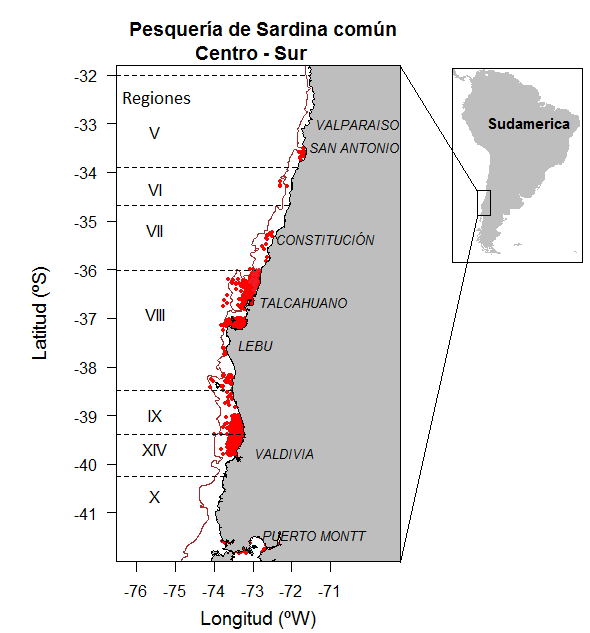
\includegraphics[width=0.8\textwidth]{FigurasInforme_Marzo/Figura1.png}
\end{center}

\small

\textbf{Figura 1}. Distribución espacial de datos provenientes del
muestreo biológico realizado por IFOP para el monitoreo de la pesquería
de sardina común. La línea color café corresponde a la isóbata de los
200 m. \vspace{0.5cm} \normalsize

\hypertarget{pesqueruxeda}{%
\subsection{2.3. Pesquería}\label{pesqueruxeda}}

Durante la década de los noventa, la flota cerquera de la zona
centro-sur incrementó significativamente las capturas de sardina común,
observándose dos importantes máximos en el año 1991 y 1999 sobrepasando
las 400 mil toneladas extraídas. Sin embargo, en los años 1993 y 1995 se
registró un fuerte descenso probablemente debido a fallas sucesivas en
los reclutamientos. Durante el período 1995 al 2000, la extracción de
pequeños pelágicos estuvo marcada por condiciones ambientales ``El
Niño'' 1997-1998 que se tradujo en alteraciones de las comunidades
costeras pelágicas, especialmente sobre el jurel, observándose una alta
e inusual presencia de ejemplares de tallas pequeñas en la pesquería
centro-sur. Este hecho generó la distorsión de los desembarques de
sardina y anchoveta durante los años 1999-2001, impulsado por evadir
multas y declarar menos jurel (Aranís 2011). Existen antecedentes que
señalan que los desembarques del primer semestre 1999 y 2000 resultan
ser muy altos para lo que en ese entonces se supone era la población de
anchoveta y sardina común. Por lo tanto, la serie de desembarques
anuales oficiales fue corregida por investigadores de IFOP, considerando
los niveles de sub-reportes de jurel durante los años 1998 - 2001, que
indican que del desembarque total informado como sardina común, menos
del 27\% correspondía efectivamente a este recurso (\textbf{Figura 2}).

\begin{center}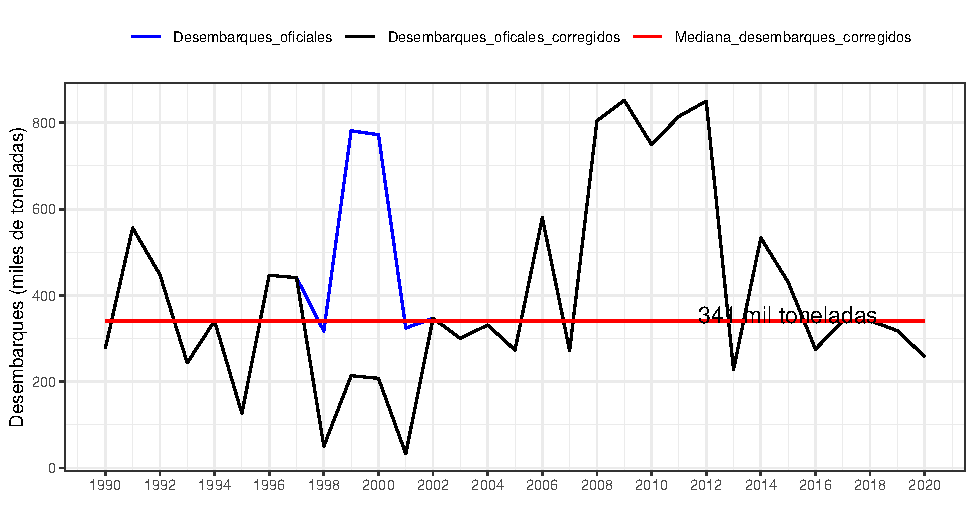
\includegraphics{FigurasInforme_Marzo/F2_ant-1} \end{center}

\vspace{-0.5cm}
\small

\textbf{Figura 2}. Desembarques (t) oficiales y corregidos de sardina
común centro-sur. \vspace{0.5cm} \normalsize

El año 2000 la pesquería es reconocida bajo régimen de plena
explotación, por lo cual se aplica la medida de administración pesquera
denominada Límite Máximo de Captura por Armador correspondiente a fijar
Cuotas Globales Anuales de Captura. Durante el período 2001 - 2005, los
desembarques se mantienen en torno a las 300 mil toneladas
(\textbf{Figura 3}). A partir del 2005 comienza un período favorable
para la condición de sardina común, ingresando a un proceso de expansión
poblacional. Esta condición permite establecer las cuotas iniciales más
altas de la serie (605 mil t), generando niveles de desembarque promedio
en torno a las 700 mil toneladas durante el período 2006 - 2012. Los
años 2001,2002, 2006, 2008, 2014 y 2017 a 2019, el desembarque artesanal
superó los niveles de cuota establecidas. Durante el 2017 el desembarque
artesanal superó en 60 mil toneladas el nivel de cuota establecida, el
2018 y 2019 fue superior en más de 100 t, mientras que el desembarque
industrial estuvo por debajo de la cuota establecida (\textbf{Figura
3}).

\begin{center}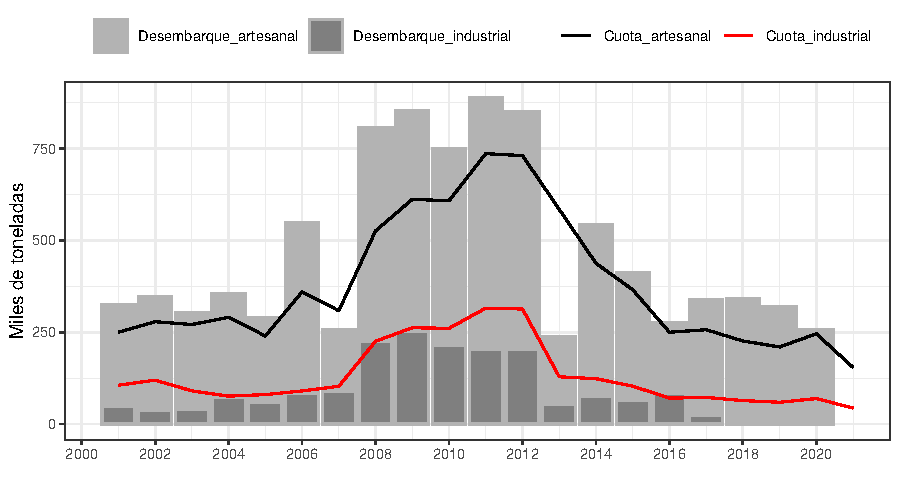
\includegraphics{FigurasInforme_Marzo/F3_ant-1} \end{center}

\vspace{-0.5cm}
\small

\textbf{Figura 3}. Relación de desembarques y cuotas anuales de sardina
común por tipo de flota. \vspace{0.5cm} \normalsize

El desembarque de sardina común se ha caracterizado por presentar un
comportamiento estacional, donde cerca del 76\% de la captura total
anual se obtiene al primer semestre de cada año, con máximos entre marzo
y abril (\textbf{Figura 4}). Esta estacionalidad está altamente
influenciada por el reclutamiento, lo que incide en un aumento de la
abundancia y disponibilidad de agregaciones de alta densidad en zonas
costeras. Producto de esta alta dependencia, la pesquería ha estado
sustentada en más del 80\% por ejemplares juveniles y reclutas
(\textbf{Figura 5}). Esto se ve reflejado en una correlación positiva
entre la biomasa acústica de enero (crucero de verano) que mide el pulso
del reclutamiento anual y los desembarques registrados al primer
semestre (\textbf{Figura 6}).

\begin{center}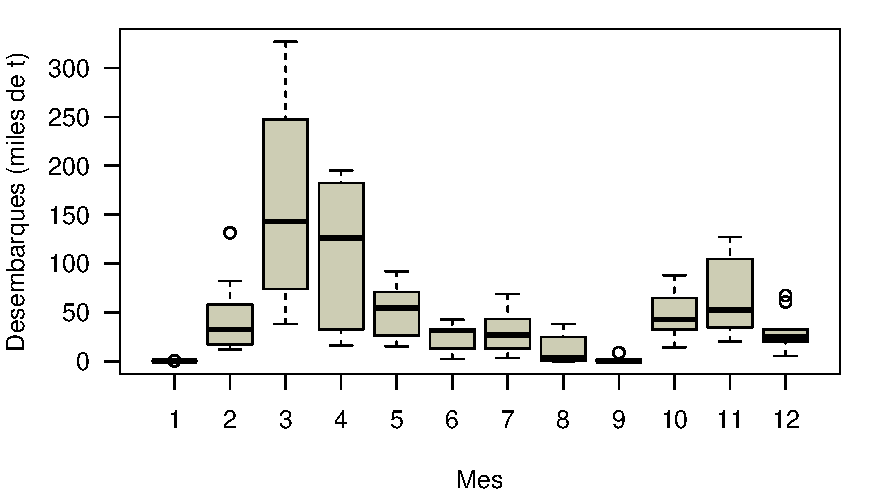
\includegraphics{FigurasInforme_Marzo/Fig4_ant-1} \end{center}

\small

\textbf{Figura 4}. Capturas mensuales de sardina común realizadas entre
2007-2016, registradas por SERNAPESCA en la zona centro-sur.
\vspace{0.5cm} \normalsize

\begin{center}
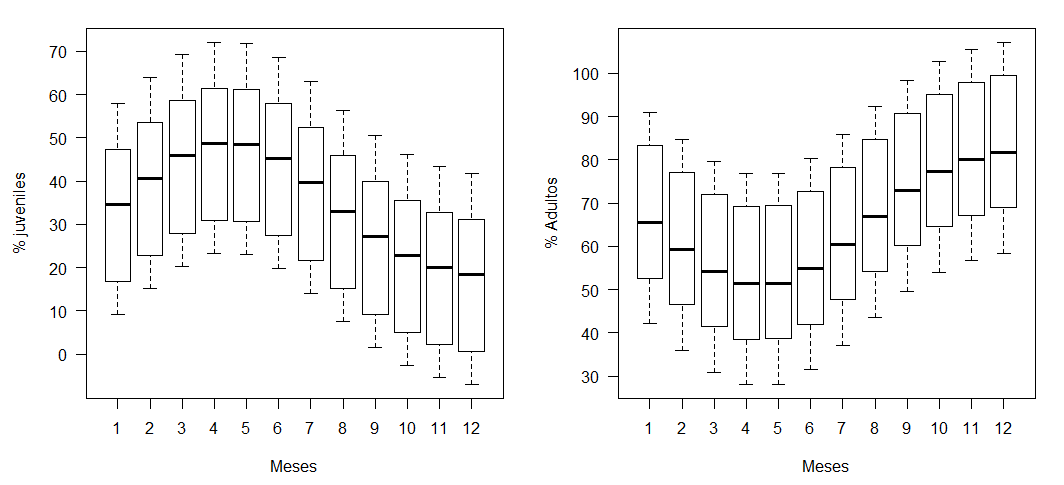
\includegraphics[width=0.95\textwidth]{FigurasInforme_Marzo/Figura5.png}
\end{center}

\small

\textbf{Figura 5}. Patrón histórico de la proporción de juveniles
(\textless11,5 cm LT) presentes en los muestreos biológicos de sardina
común en la flota total centro-sur. \vspace{0.5cm}

\begin{center}
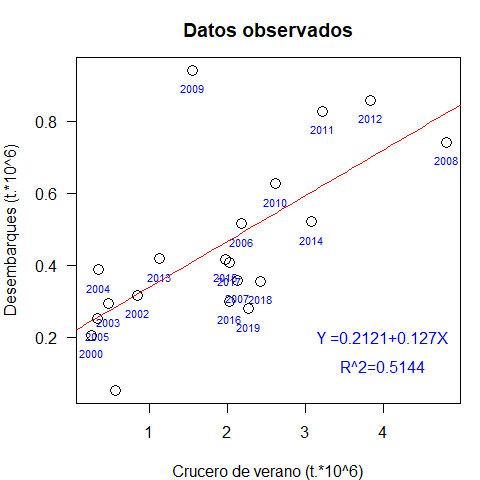
\includegraphics[width=0.6\textwidth]{FigurasInforme_Marzo/Figura6.png}
\end{center}

\small

\textbf{Figura 6}. Relación entre desembarques registrados durante el
primer semestre de cada año versus la biomasa acústica de verano (enero)
del mismo año. \vspace{0.5cm}

\normalsize

\hypertarget{reclutamiento}{%
\subsection{2.3. Reclutamiento}\label{reclutamiento}}

Las áreas de reclutamiento se ubican principalmente frente a la Región
del Biobío, concentrándose fundamentalmente al norte de Isla Mocha. Las
condiciones ambientales que afectan a este proceso se vinculan con
ciertas masas de agua, anomalías de las variables (Temperatura,
Salinidad, Oxígeno disuelto, gradientes, etc.), intensidad de los
vientos y el nivel de los procesos vinculados (índice de surgencia,
índices de turbulencia, transporte de Ekman, etc) (Yáñez \emph{et al}.
2005; Castillo \emph{et al}. 2013).

En este sentido, Castillo \emph{et al}. (2013) encontraron una relación
negativa entre la densidad de anchoveta y sardina común de la zona
centro-sur y el índice de turbulencia (del invierno anterior al
reclutamiento), debido a la advección de huevos y larvas lejos de la
costa. Además, la intensidad de la surgencia costera frente a Chile
centro - sur experimenta una alta variabilidad interanual que está
modulado por ENOS. El impacto de ENOS en el sistema de surgencia se
relaciona principalmente con teleconexiones atmosféricas (Montecinos \&
Gómez, 2010). Gómez \emph{et al}. (2012) encontraron que la surgencia
impulsada por el viento y El Niño 3.4 se correlaciona significativamente
con la clorofila y los reclutamientos. Además, identificaron que cuando
la surgencia es débil la clorofila costera es baja, el reclutamiento es
bajo y la tasa de supervivencia de reclutas es baja. De este modo, estos
autores sugieren que la clorofila costera de primavera es un buen
indicador de la abundancia de alimento de sardina común, afectando
significativamente la supervivencia de pre-reclutas de sardina común y
por consiguiente, la fuerza de los reclutamientos a finales de
primavera. Otros autores han encontrado una relación inversa y
significativa con la anomalía de la TSM y una relación positiva y
significativa con la anomalía de la CHL, ya que se reconoce que la
sardina común se alimenta preferentemente sobre presas de menor tamaño
asociadas al fitoplancton (Arteaga \emph{et al}. 2014, Cubillos \& Arcos
2002, Van der Lingen \emph{et al}. 2009).

Para evaluar la magnitud del reclutamiento anual se realiza la
evaluación hidroacústica desde el año 2000, en enero de cada año donde
se maximiza la presencia de juveniles de sardina común y anchoveta en la
zona centro-sur. A partir del 2003 se replicó la prospección en otoño
(mayo) para incrementar la certeza de la estimación haciendo un
seguimiento de la evolución del proceso o para capturar un eventual
segundo pulso, especialmente en anchoveta. De este modo, ha sido posible
establecer una estacionalidad en la composición específica de las
biomasas de estas dos especies, en verano la sardina domina respecto a
la anchoveta mientras que en el otoño se presenta un incremento relativo
de la anchoveta y una reducción en la sardina junto a cambios en su
distribución geográfica (Castillo \emph{et al}. 2013). La serie de
biomasas se caracteriza por presentar una menor abundancia promedio
durante el otoño respecto de las estimaciones de verano, producto de
factores asociados a la pesca y a la menor disponibilidad que
experimenta el recurso hacia mitad de año. Sin embargo, la distribución
espacial de los últimos años se ha visto alterada producto de ``El
Niño'' 2016, observándose una relación positiva, aunque no
significativa, entre ambos cruceros (\textbf{Figura 7}).

\begin{center}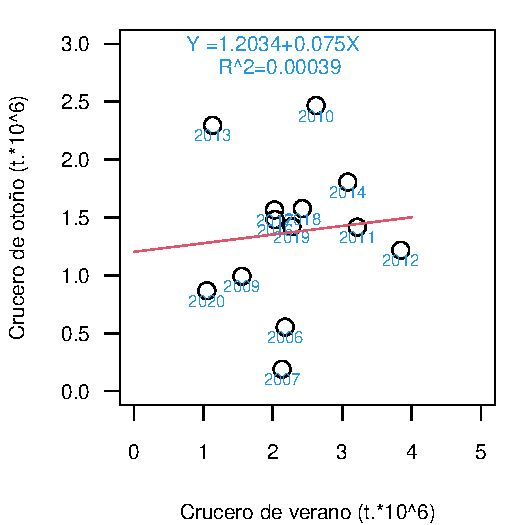
\includegraphics{FigurasInforme_Marzo/Fig7_ant_reclutas-1} \end{center}

\small

\textbf{Figura 7}. Relación entre la biomasa total del crucero acústico
de otoño versus la biomasa total del crucero acústico de verano (enero)
del mismo año para sardina común. \vspace{0.5cm} \normalsize

Se ha observado una gran variabilidad interanual asociada a la fortaleza
del pulso de reclutamiento de ambos recursos. A partir del 2005 la
biomasa exhibe un importante aumento con un máximo histórico de 4,8
millones de toneladas el año 2008, el cual se mantiene hasta el verano
del 2012 (3,8 millones de t). El período favorable de la sardina
iniciado el 2005, coincide con el dominio en la zona de anomalías
térmicas superficiales negativas, que se han presentado con intensidad
variable (Castillo \emph{et al}. 2012). Esta tendencia cambia el 2013
(1.133.477 t.) representando una reducción superior al 239\% en
comparación al verano del 2012; 185\% en relación al 2011 y 131\%
respecto al 2010. En relación a la abundancia de ejemplares menores a
11,5 cm sólo representó el 42,5\% del total, con un descenso
significativo (63,9\%), respecto de los meses de enero y mayo del 2012,
períodos en los cuales la participación de reclutas superó el 88\%. Esta
condición se revierte el año 2014, con una importante recuperación de la
biomasa total estimada en 3.079.434 t. y de la presencia de reclutas con
una abundancia de ejemplares menores a 11,5 cm que representó el 96,4\%
del total (740 mil millones). Sin embargo, a partir del 2015 las
biomasas acústicas se mantienen en torno a los 2 millones de toneladas y
con disminución de la biomasa de reclutas en el año 2019. El crucero de
verano 2020 estimó una dismunición de la biomasa total y de reclutas en
torno al 50\% y 80\% respectivamente, respecto de las estimadas el año
anterior, No obstante, se registra una recuperación de los niveles de
biomasa total, retornando a niveles en torno a los 2 millones de
toneladas (\textbf{Figura 8}).

\begin{center}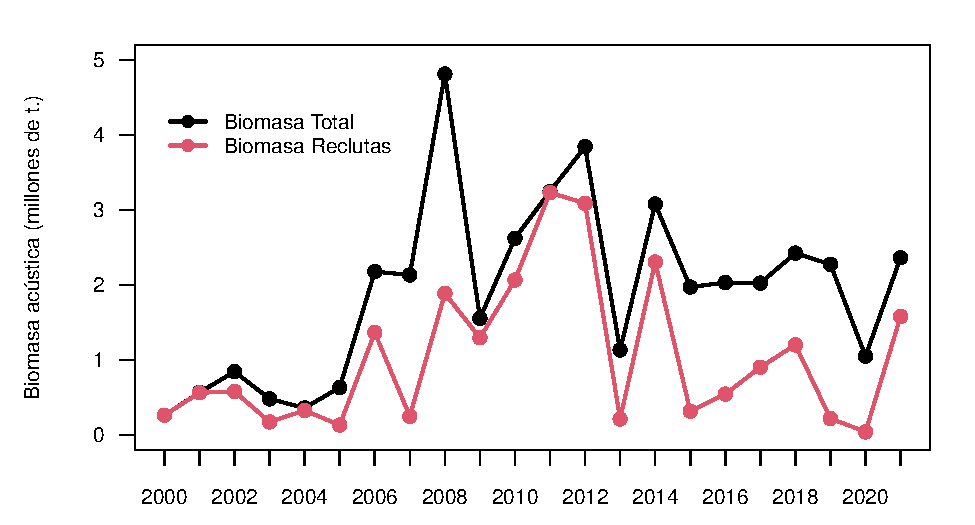
\includegraphics{FigurasInforme_Marzo/Fig8_ant_reclutasbio-1} \end{center}

\small

\textbf{Figura 8}. Biomasa acústica total y de reclutas (\textless11,5
cm) de sardina común centro-sur. \vspace{0.5cm} \normalsize

\hypertarget{reproducciuxf3n}{%
\subsection{2.4. Reproducción}\label{reproducciuxf3n}}

Los peces pelágicos pequeños adaptan su ciclo reproductivo desovando en
zonas protegidas y/o períodos del año favorables para la sobrevivencia y
desarrollo de estadíos tempranos (Parrish \emph{et al}. 1983, Hutchings
\emph{et al}. 1998, Cubillos \emph{et al}. 2001). El área de desove de
sardina común y anchoveta de las regiones de Valparaíso a Los Lagos, se
ubica principalmente en la zona de Lebu-Corral, la cual correspondería a
una zona de pre-reclutamiento/desove con un alto nivel de retención
(\textbf{Figura 9}) producto de una alternancia entre convergencias
costeras producidas por vientos norte que favorecerían la concentración
y retención en la costa y vientos sur que promoverían el enriquecimiento
de aguas costeras con eventos de surgencia de moderada intensidad
(Cubillos \emph{et al}. 2011, Parada \emph{et al}. 2012, Soto-Mendosa
\emph{et al}. 2012).

La sardina común presenta un desove parcial o fraccionado, es decir, el
total de ovocitos maduros producidos por una hembra son expulsados en
grupos o modas sucesivas durante la temporada de desove, registrando
actividad reproductiva a lo largo de todo el año, con un período de
máxima actividad reproductiva centrada entre los meses de agosto y hasta
octubre, período en que las condiciones oceanográficas exhiben una
transición entre un régimen de convergencias costeras (transporte hacia
la costa) y un régimen de surgencias moderadas que permiten la
concentración y retención de huevos en la costa y la provisión de
alimento para la supervivencia de las larvas. El período de inactividad
o reposo reproductivo se registra durante los primeros meses del año
(enero -- mayo) y hacia fines de año (noviembre y diciembre) reflejado
en los bajos valores del IGS y PHA mostrados en la \textbf{Figura 10}. A
través del tiempo, este proceso ha tendido a focalizar su máxima
actividad hacia primavera, centrando el desove entre agosto - noviembre.
Por lo tanto, la estacionalidad del proceso reproductivo de esta especie
no es estático temporalmente con una fecha de inicio, desarrollo y final
predeterminado.

El proceso reproductivo ha sido de mayor extensión, magnitud y
anticipación entre julio y principios de agosto durante los años 2011 y
2012 respecto del patrón histórico, explicando una mayor intensión
reproductiva. Sin embargo, el año 2013 a 2016 el adelantamiento se
observa hacia fines del mes de junio. La fluctuación de IGS y PHA indica
que la época de desove se extendió entre junio y noviembre de 2013 al
2015, concentrándose la máxima actividad reproductiva en julio y
octubre. Los cambios en la duración de los períodos de desove podrían
estar relacionados con la calidad y cantidad de los alimentos en el
verano anterior, que a su vez determina la energía disponible para la
reproducción, afectando la calidad de la descendencia (Claramunt
\emph{et al}. 2013, Castro \emph{et al}. 2009, 2010). En estos recursos
se debe considerar también que la estación reproductiva se encuentra
fuertemente influenciada por la longitud de las hembras, así, cambios en
la estructura de talla determinan potencialmente cambios intra e
interanuales en la duración e intensidad del proceso de desove.

\begin{center}
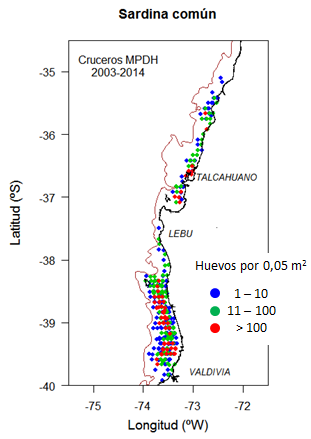
\includegraphics[width=1.1\textwidth]{FigurasInforme_Marzo/Figura9.png}
\end{center}

\small

\textbf{Figura 9}. Distribución de huevos recolectados en Cruceros de
huevos (MPDH, 2003 - 2014) de sardina común en la Zona Centro-Sur de
Chile. La línea café representa isobata de 200 m. \vspace{0.5cm}
\normalsize

\begin{center}
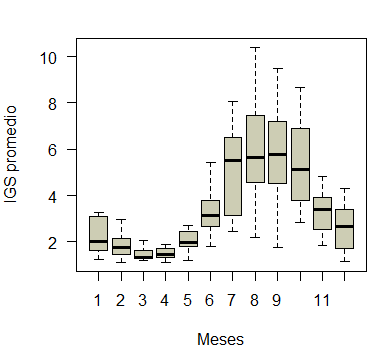
\includegraphics[width=0.5\textwidth]{FigurasInforme_Marzo/Figura10a.png}
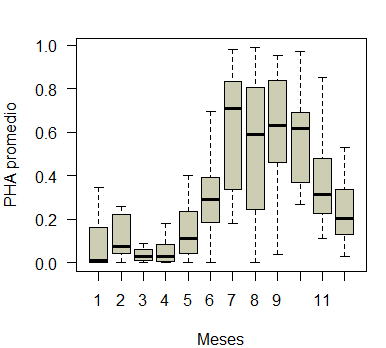
\includegraphics[width=0.5\textwidth]{FigurasInforme_Marzo/Figura10b.png}
\end{center}

\small

\textbf{Figura 10}. Variación promedio mensual del índice gonadosomático
(IGS) y proporción de hembras activas (PHA) de las hembras de sardina
común de la zona de San Antonio-Valdivia entre los años 2001 a 2016.
\vspace{0.5cm} \normalsize

\hypertarget{evaluaciuxf3n-de-stock}{%
\subsection{2.6. Evaluación de stock}\label{evaluaciuxf3n-de-stock}}

La evaluación de stock desarrollada por IFOP se encuentra en general
acorde con los estándares internacionales vigentes. A su vez, las
pesquerías han sido clasificados en grupos de calidad o \emph{``Tiers''}
conforme el nivel de conocimiento, cantidad y calidad de la información
disponible que aporta la evaluación de stock. Se ha tomado en
consideración las recomendaciones emanadas tanto desde los Comités
Científico Técnicos como de los lineamientos entregados por el equipo de
expertos nacionales e internacionales en el marco del proyecto
``Revisión de los puntos biológicos de referencia (Rendimiento Máximo
Sostenido) en las pesquerías nacionales'' (Payá \emph{et al}. 2014). En
el desarrollo de (los) método(s) y modelo(s) empleados se consideran
elementos de incertidumbre estructural basados en el nivel de
conocimiento y de la información o datos disponible, así como la
incertidumbre de estimación generada de su aplicación al conjunto de
datos disponibles. Independientemente del nivel del estándar, en base al
permanente proceso de mejora se recomendará la realización de estudios,
cruceros, investigaciones, monitoreo y otras acciones conducentes a
mejorar el estado de conocimiento del recurso en cuestión y la
pesquería, con el fin de allanar las brechas de conocimiento e
información conducentes a reducir los niveles de incertidumbre.

El stock de sardina común comenzó a ser evaluado con métodos
estructurados por edad. La \textbf{Tabla 1} muestra las características
que ha tenido la evolución en la modelación de dinámica poblacional en
los últimos 18 años. En términos del lenguaje de programación, por más
de 10 años, Excel y MATLAB fueron la plataforma en que se implementaron
modelos de dinámica en edades en escala anual y semestral, con
observaciones en tallas y edades. En el año 2010 se inició la migración
de los modelos hacia el lenguaje ADMB (Fournier \emph{et al}. 2012) con
lo cual IFOP actualmente utiliza el mismo lenguaje que en la costa oeste
de EE.UU, facilitando la revisión por pares desde esa región.

\small
\begin{center} 
\textbf{Tabla 1.}
\end{center}
\begin{center} 
\vspace{-0.2cm} Evolución de los modelos de evaluación empleados en sardina común centro-sur.
\end{center}
\vspace{-0.2cm}

\begin{table}[h]
    \centering
    \resizebox{13cm}{!} {
    \begin{tabular}{|l|l|c|c|}
    \hline
Años       & Modelo                               & Plataforma   & Índices   \\ \hline   
<2000      & Producción excedentaria              & Excel        & CPUE      \\ \hline
           &                                      &              &           \\ 
2000-2005  & Anual edad-estructurado (MAE)        & MATLAB       & CPUE      \\
           &                                      &              & RECLAS    \\ \hline        
           & Anual edad-estructurado (MAE),       &              & CPUE      \\
2005-2010  & Anual talla-estructurado (MAT),      & MATLAB       & RECLAS    \\
           & Semestral talla-estructurado (MST)   &              & PELACES   \\ \hline
           &                                      &              &           \\
2010-2012  & Anual edad-estructurado (MAE)        & ADMB         & RECLAS    \\
           & Semestral talla-estructurado (MST)   &              & PELACES   \\ \hline
           &                                      &              & RECLAS    \\
2012-2013  & Anual edad-estructurado (MAE)        & ADMB         & PELACES   \\
           &                                      &              & MPH       \\ \hline
           &                                      &              &           \\
2014-2020  & Anual edad-estructurado (MAE)        & ADMB         & RECLAS    \\
           &                                      &              & PELACES   \\ \hline
  \end{tabular}}
        \end{table}

\normalsize

En base al modelo conceptual de la dinámica del stock de sardina común
se sustenta el enfoque y modelo de evaluación, que permite asesorar al
Comité Científico Técnico de Pesquerías de Pequeños Pelágicos (CCT-PP)
en los análisis de la productividad del stock y de sus posibilidades de
explotación, considerando los parámetros e indicadores estimados por el
modelo de evaluación de sardina común con su incertidumbre asociada.

\hypertarget{captura-bioluxf3gicamente-aceptable-cba}{%
\subsection{2.7. Captura Biológicamente Aceptable
(CBA)}\label{captura-bioluxf3gicamente-aceptable-cba}}

De acuerdo al ciclo de manejo histórico de esta pesquería, la
recomendación de CBA comienza con el cálculo de la CBA inicial que
permite al CCT-PP, establecer el estatus y recomendar el rango de CBA
para el año siguiente. En enero de cada año, el crucero de evaluación
hidroacústico permite estimar la abundancia y biomasa de reclutas
(crucero de verano), esta información junto a datos provenientes de la
pesquería (del año anterior) es utilizada para la primera revisión de la
CBA. En marzo se inicia el período de extracción y en mayo se realiza el
segundo crucero de evaluación acústica (crucero de otoño) para
actualizar el estatus y revisar una vez más la CBA.

El año 2013 se realizó el establecimiento del nuevo Reglamento (D:S: N°
77, Mayo 2013) dispuesto en la Ley General de Pesca y Acuicultura (LGPA)
que establece que las pesquerías deberán alcanzar o mantenerse en torno
del Rendimiento Máximo Sostenido (RMS) considerando las características
biológicas de los recursos explotados. La nueva LGPA establece que el
Comité Científico Técnico será quien recomiende el marco biológico de
referencia, estatus de conservación biológica y rango de captura
biológicamente aceptable (CBA). Este hecho coincide con la fuerte caída
en el desembarque (232 mil t), disminuyendo un 73\% respecto al año
2012, producto de una falla del reclutamiento en el 2013.

En consecuencia, considerando la caída del reclutamiento 2013, el CTT-PP
recomienda una CBA inicial 2014 (establecida en diciembre 2013) de 373
mil toneladas. En marzo del 2014, se re-calculó la CBA con la
información entregada por el crucero de evaluación hidroacústica de
enero, que arrojó un incremento de la biomasa acústica, permitiendo
aumentar la CBA a 572 mil toneladas (t) para el mismo año. Del
desembarque total registrado el 2014 (543 mil t) un 77\% fue capturado
entre los meses de enero y junio.

Para el año 2015 se recomendó una CBA inicial de 323 mil t, en marzo del
2015 se re-calculó con información del crucero de enero 2015 que arrojó
una disminución en la presencia de reclutas por lo tanto la CBA se
incrementa levemente a 356 mil t. En junio 2015 se re-calcula nuevamente
con información del crucero de mayo 2015 que arrojó un aumento de la
biomasa acústica permitiendo un incremento en la CBA 2015 a 478 mil t.
Del desembarque total registrado el 2015 (430 mil t) un 64\% fue
capturado entre los meses de enero-junio.

Debido a la alta incertidumbre en el nivel del reclutamiento 2016, la
CBA inicial 2016 recomendada por el CCT-PP bajo un enfoque precautorio
fue de 286 mil t, la cual fue incrementada luego de la actualización con
información del crucero de enero 2016 a 326 mil t. Sin embargo, los
desembarques registrados para el año 2016 sólo alcanzaron las 275 mil
toneladas, donde un 51\% fue capturado entre los meses de enero-junio
(\textbf{Tabla 2}). Esta disminución en las capturas se asocia a la
presencia del evento ``El Niño 2015-2016'' que afectaría a la
distribución relativa del stock. Aranís \emph{et al}. (2016) señalaron
que el recurso no estaría accesible a la flota artesanal de la Región
del Biobío provocando una baja importante en las capturas y rendimientos
de pesca. Continuando con el enfoque precautorio, la recomendación para
la CBA inicial 2017 fue de 273 mil toneladas, la cual fue incrementada
luego de la actualización con información del crucero de verano 2017 a
310 mil t y luego con información del crucero de otoño 2017 a 336 mil t.
Para el año 2018, la CBA inicial recomendada incorpora un 4\% de
descarte y, por lo tanto, queda establecida en 296 mil t. Luego de la
primera actualización de marzo se incrementa la cuota a 321 mil t. Para
el año 2019 la CBA inicial recomendada incorpora un 2\% de descarte,
estableciéndose en 274 mil t, la primera actualización de marzo se
incrementa la cuota a 335 mil t y en agosto se incrementa a 337 mil t.
Durante el 2019 se capturó un 95\% de la CBA recomendada en agosto 2019.

Para el año 2020 la CBA inicial recomendada incorpora un 2\% de
descarte, estableciéndose en 321 mil t, considerando por primera vez una
probabilidad de sobrepasar el objetivo de manejo del 40\% (lo general
era utilizar un 30\% de probabilidad). En la primera y segunda
actualización de marzo y julio los resultados de la evaluación de stock
arrojaron menores estimados de captura debido a la disminución de los
reclutamientos de los últimos años y de las biomasas registradas por los
cruceros acústicos. Desde un punto de vista práctico y administrativo es
imposible disminuir la cuota asignada, aunque se cuente con información
actualizada y estimados de estatus y CBA más confliables, esto debido a
que por lo general a mitad de año gran parte de la cuota ha sido
consumida. Ante esta situación el CCT-PP ha recomendado mantener una
situación de ``statu quo'' cada vez que se ha presentado una disminución
de la CBA en el segundo y/o tercer hito del ciclo de manejo. No
obstante, a junio del 2020 se ha capturado tan sólo 59\% de la CBA
recomendada, lo general es que se captura sobre un 70\% el primer
semestre del año. Esta reducción en los niveles de captura tienen al
parecer tiene relación con la disminución de los niveles de biomasa de
sardina común como a la condición de pandemia que ha disminuido el
esfuerzo pesquero en la zona centro-sur de Chile.

\pagebreak

\small
\begin{center} 
\textbf{Tabla 2.}
\end{center}
\begin{center} 
\vspace{-0.2cm} Capturas biológicamente aceptables recomendadas por el CCT-PP en 
las distintas etapas de establecimiento de CBA y estatus de sardina común y el Desembarque registrado.
\end{center}
\vspace{-0.2cm}

\begin{longtable}[]{@{}ccccc@{}}
\toprule
\begin{minipage}[b]{0.08\columnwidth}\centering
Año\strut
\end{minipage} & \begin{minipage}[b]{0.18\columnwidth}\centering
CBA inicial

(miles de t.)\strut
\end{minipage} & \begin{minipage}[b]{0.22\columnwidth}\centering
1era revisión CBA

(miles de t.)\strut
\end{minipage} & \begin{minipage}[b]{0.21\columnwidth}\centering
2da revisión CBA

(miles de t.)\strut
\end{minipage} & \begin{minipage}[b]{0.18\columnwidth}\centering
Desembarques

(miles de t.)\strut
\end{minipage}\tabularnewline
\midrule
\endhead
\begin{minipage}[t]{0.08\columnwidth}\centering
2014\strut
\end{minipage} & \begin{minipage}[t]{0.18\columnwidth}\centering
373\strut
\end{minipage} & \begin{minipage}[t]{0.22\columnwidth}\centering
572\strut
\end{minipage} & \begin{minipage}[t]{0.21\columnwidth}\centering
-\strut
\end{minipage} & \begin{minipage}[t]{0.18\columnwidth}\centering
543\strut
\end{minipage}\tabularnewline
\begin{minipage}[t]{0.08\columnwidth}\centering
2015\strut
\end{minipage} & \begin{minipage}[t]{0.18\columnwidth}\centering
323\strut
\end{minipage} & \begin{minipage}[t]{0.22\columnwidth}\centering
356\strut
\end{minipage} & \begin{minipage}[t]{0.21\columnwidth}\centering
478\strut
\end{minipage} & \begin{minipage}[t]{0.18\columnwidth}\centering
430\strut
\end{minipage}\tabularnewline
\begin{minipage}[t]{0.08\columnwidth}\centering
2016\strut
\end{minipage} & \begin{minipage}[t]{0.18\columnwidth}\centering
286\strut
\end{minipage} & \begin{minipage}[t]{0.22\columnwidth}\centering
326\strut
\end{minipage} & \begin{minipage}[t]{0.21\columnwidth}\centering
326\strut
\end{minipage} & \begin{minipage}[t]{0.18\columnwidth}\centering
275\strut
\end{minipage}\tabularnewline
\begin{minipage}[t]{0.08\columnwidth}\centering
2017\strut
\end{minipage} & \begin{minipage}[t]{0.18\columnwidth}\centering
273\strut
\end{minipage} & \begin{minipage}[t]{0.22\columnwidth}\centering
310\strut
\end{minipage} & \begin{minipage}[t]{0.21\columnwidth}\centering
336\strut
\end{minipage} & \begin{minipage}[t]{0.18\columnwidth}\centering
335\strut
\end{minipage}\tabularnewline
\begin{minipage}[t]{0.08\columnwidth}\centering
2018\strut
\end{minipage} & \begin{minipage}[t]{0.18\columnwidth}\centering
296\strut
\end{minipage} & \begin{minipage}[t]{0.22\columnwidth}\centering
321\strut
\end{minipage} & \begin{minipage}[t]{0.21\columnwidth}\centering
-\strut
\end{minipage} & \begin{minipage}[t]{0.18\columnwidth}\centering
341\strut
\end{minipage}\tabularnewline
\begin{minipage}[t]{0.08\columnwidth}\centering
2019\strut
\end{minipage} & \begin{minipage}[t]{0.18\columnwidth}\centering
274\strut
\end{minipage} & \begin{minipage}[t]{0.22\columnwidth}\centering
335\strut
\end{minipage} & \begin{minipage}[t]{0.21\columnwidth}\centering
337\strut
\end{minipage} & \begin{minipage}[t]{0.18\columnwidth}\centering
318\strut
\end{minipage}\tabularnewline
\begin{minipage}[t]{0.08\columnwidth}\centering
2020\strut
\end{minipage} & \begin{minipage}[t]{0.18\columnwidth}\centering
321\strut
\end{minipage} & \begin{minipage}[t]{0.22\columnwidth}\centering
321\strut
\end{minipage} & \begin{minipage}[t]{0.21\columnwidth}\centering
321\strut
\end{minipage} & \begin{minipage}[t]{0.18\columnwidth}\centering
258\strut
\end{minipage}\tabularnewline
\begin{minipage}[t]{0.08\columnwidth}\centering
2021\strut
\end{minipage} & \begin{minipage}[t]{0.18\columnwidth}\centering
201\strut
\end{minipage} & \begin{minipage}[t]{0.22\columnwidth}\centering
-\strut
\end{minipage} & \begin{minipage}[t]{0.21\columnwidth}\centering
-\strut
\end{minipage} & \begin{minipage}[t]{0.18\columnwidth}\centering
-\strut
\end{minipage}\tabularnewline
\bottomrule
\end{longtable}

\pagebreak
\normalsize

\hypertarget{metodologuxeda-de-trabajo}{%
\section{3. METODOLOGÍA DE TRABAJO}\label{metodologuxeda-de-trabajo}}

\hypertarget{objetivo-especuxedfico-1}{%
\subsection{3.1. Objetivo específico
1:}\label{objetivo-especuxedfico-1}}

\vspace{-0.2cm}

\emph{``Implementar procedimientos de evaluación de stock basados en
protocolos científicos para la determinación del estatus de sardina
común, con arreglo al nivel de información, conocimiento e incertidumbre
correspondiente, conforme a los estándares actuales en ciencia
pesquera.''}

\hypertarget{modelo-conceptual}{%
\subsubsection{3.1.1. Modelo Conceptual}\label{modelo-conceptual}}

La conceptualización del modelo biológico considera los siguientes
componentes de la dinámica poblacional:

\begin{itemize}
\tightlist
\item
  Estructura geográfica: Se asume que la población de sardina común
  entre las Regiones de Valparaíso y Biobío constituye una unidad de
  stock. Se asume un stock homogéneo al interior de la unidad de
  pesquería, donde el conjunto de individuos está sujeto a la misma
  probabilidad de crecimiento y mortalidad, y donde la migración no es
  importante.
\item
  Reproducción: Se asume que los individuos del stock tienen un evento
  reproductivo discreto, que se representa a comienzos de la estación
  reproductiva y que con propósitos prácticos ocurre en agosto.
\item
  Reclutamiento: El reclutamiento ocurre a la forma de un pulso de
  abundancia en enero de cada año, 5 meses después del evento
  reproductivo.
\item
  Tasa de mortalidad natural: La tasa de mortalidad natural se asume
  invariante y se considera M=1,0 por año para sardina común.
\item
  Dinámica del crecimiento: El crecimiento intra-anual es recogido en
  dos matrices de pesos medios a la edad, las que corresponden
  respectivamente a las estimaciones a mitad de año (enero) luego de la
  asignación de la edad, y las estimaciones de pesos iniciales del año
  (julio).
\end{itemize}

El modelo de evaluación de stock de sardina común se basa en un análisis
estadístico de la dinámica de estructuras de edad anual que incorpora
información biológica y pesquera agregada en año biológico. La
información que ingresa al modelo consiste en los desembarques totales
obtenidos de los registros oficiales de SERNAPESCA los cuales son
convertidos a temporada de pesca considerando la estacionalidad de la
pesquería, los datos de composición de edad anual y pesos medios a la
edad de la flota son proporcionados por el programa de monitoreo de las
pesquerías de peces pelágicos, mientras que las evaluaciones
hidroacústicas de verano y otoño proporcionan información de biomasa de
reclutas en verano y biomasa vulnerable en otoño junto con sus
respectivas composiciones de edad. En base a esta información el modelo
estima las variables de estado representadas por la biomasa desovante
(BD) y los niveles de mortalidad por pesca (F), que junto a los puntos
biológicos de referencia (PBRs), permiten determinar el estatus y
calcular la Captura Biológicamente Aceptable (CBA) (\textbf{Figura 11}).

\begin{center}

\includegraphics[width=1\textwidth]{FigurasInforme_Marzo/Figura11.png}
\end{center}

\small

\textbf{Figura 11}. Procedimiento de evaluación de stock de sardina
común centro-sur. \vspace{0.5cm} \normalsize

En la implementación del procedimiento de evaluación de stock se
utilizan protocolos científicos basados en la determinación de un
sistema de niveles o ``tiers'' que permiten clasificar la información
disponible de las especies y su pesquería, los cuales se han convertido
en una herramienta de uso común en la asesoría orientada al manejo
pesquero en la actualidad. Para estimar el RMS se utiliza la estrategia
de niveles y de acuerdo con la clasificación del estándar de información
se definen los PBR o ``proxy'' que serán usados para determinar el
estatus del recurso. La definición de los procedimientos de cálculo de
los PBR y del marco de referencia especie específicos se basan en el
estudio ``Revisión de los puntos Biológicos de referencia (Rendimiento
Máximo Sostenible) en las pesquerías nacionales'' (Paya \emph{et al}.
2014), en cuyo primer taller, se desarrolló en conjunto con expertos
internacionales, un sistema de tres niveles para derivar al RMS
específico para las pesquerías en Chile (\textbf{Figura 12}). Además,
para determinar el estatus de los recursos selectos, se considera lo
establecido por el Comité Científico Técnico de Pelágicos Pequeños
(CCT-PP) sobre los requerimientos técnicos que define los estándares de
análisis y evaluación para las pesquerías analizadas, conforme a los
niveles de conocimiento, información y calidad de los datos disponibles
para esos fines.

\begin{center}
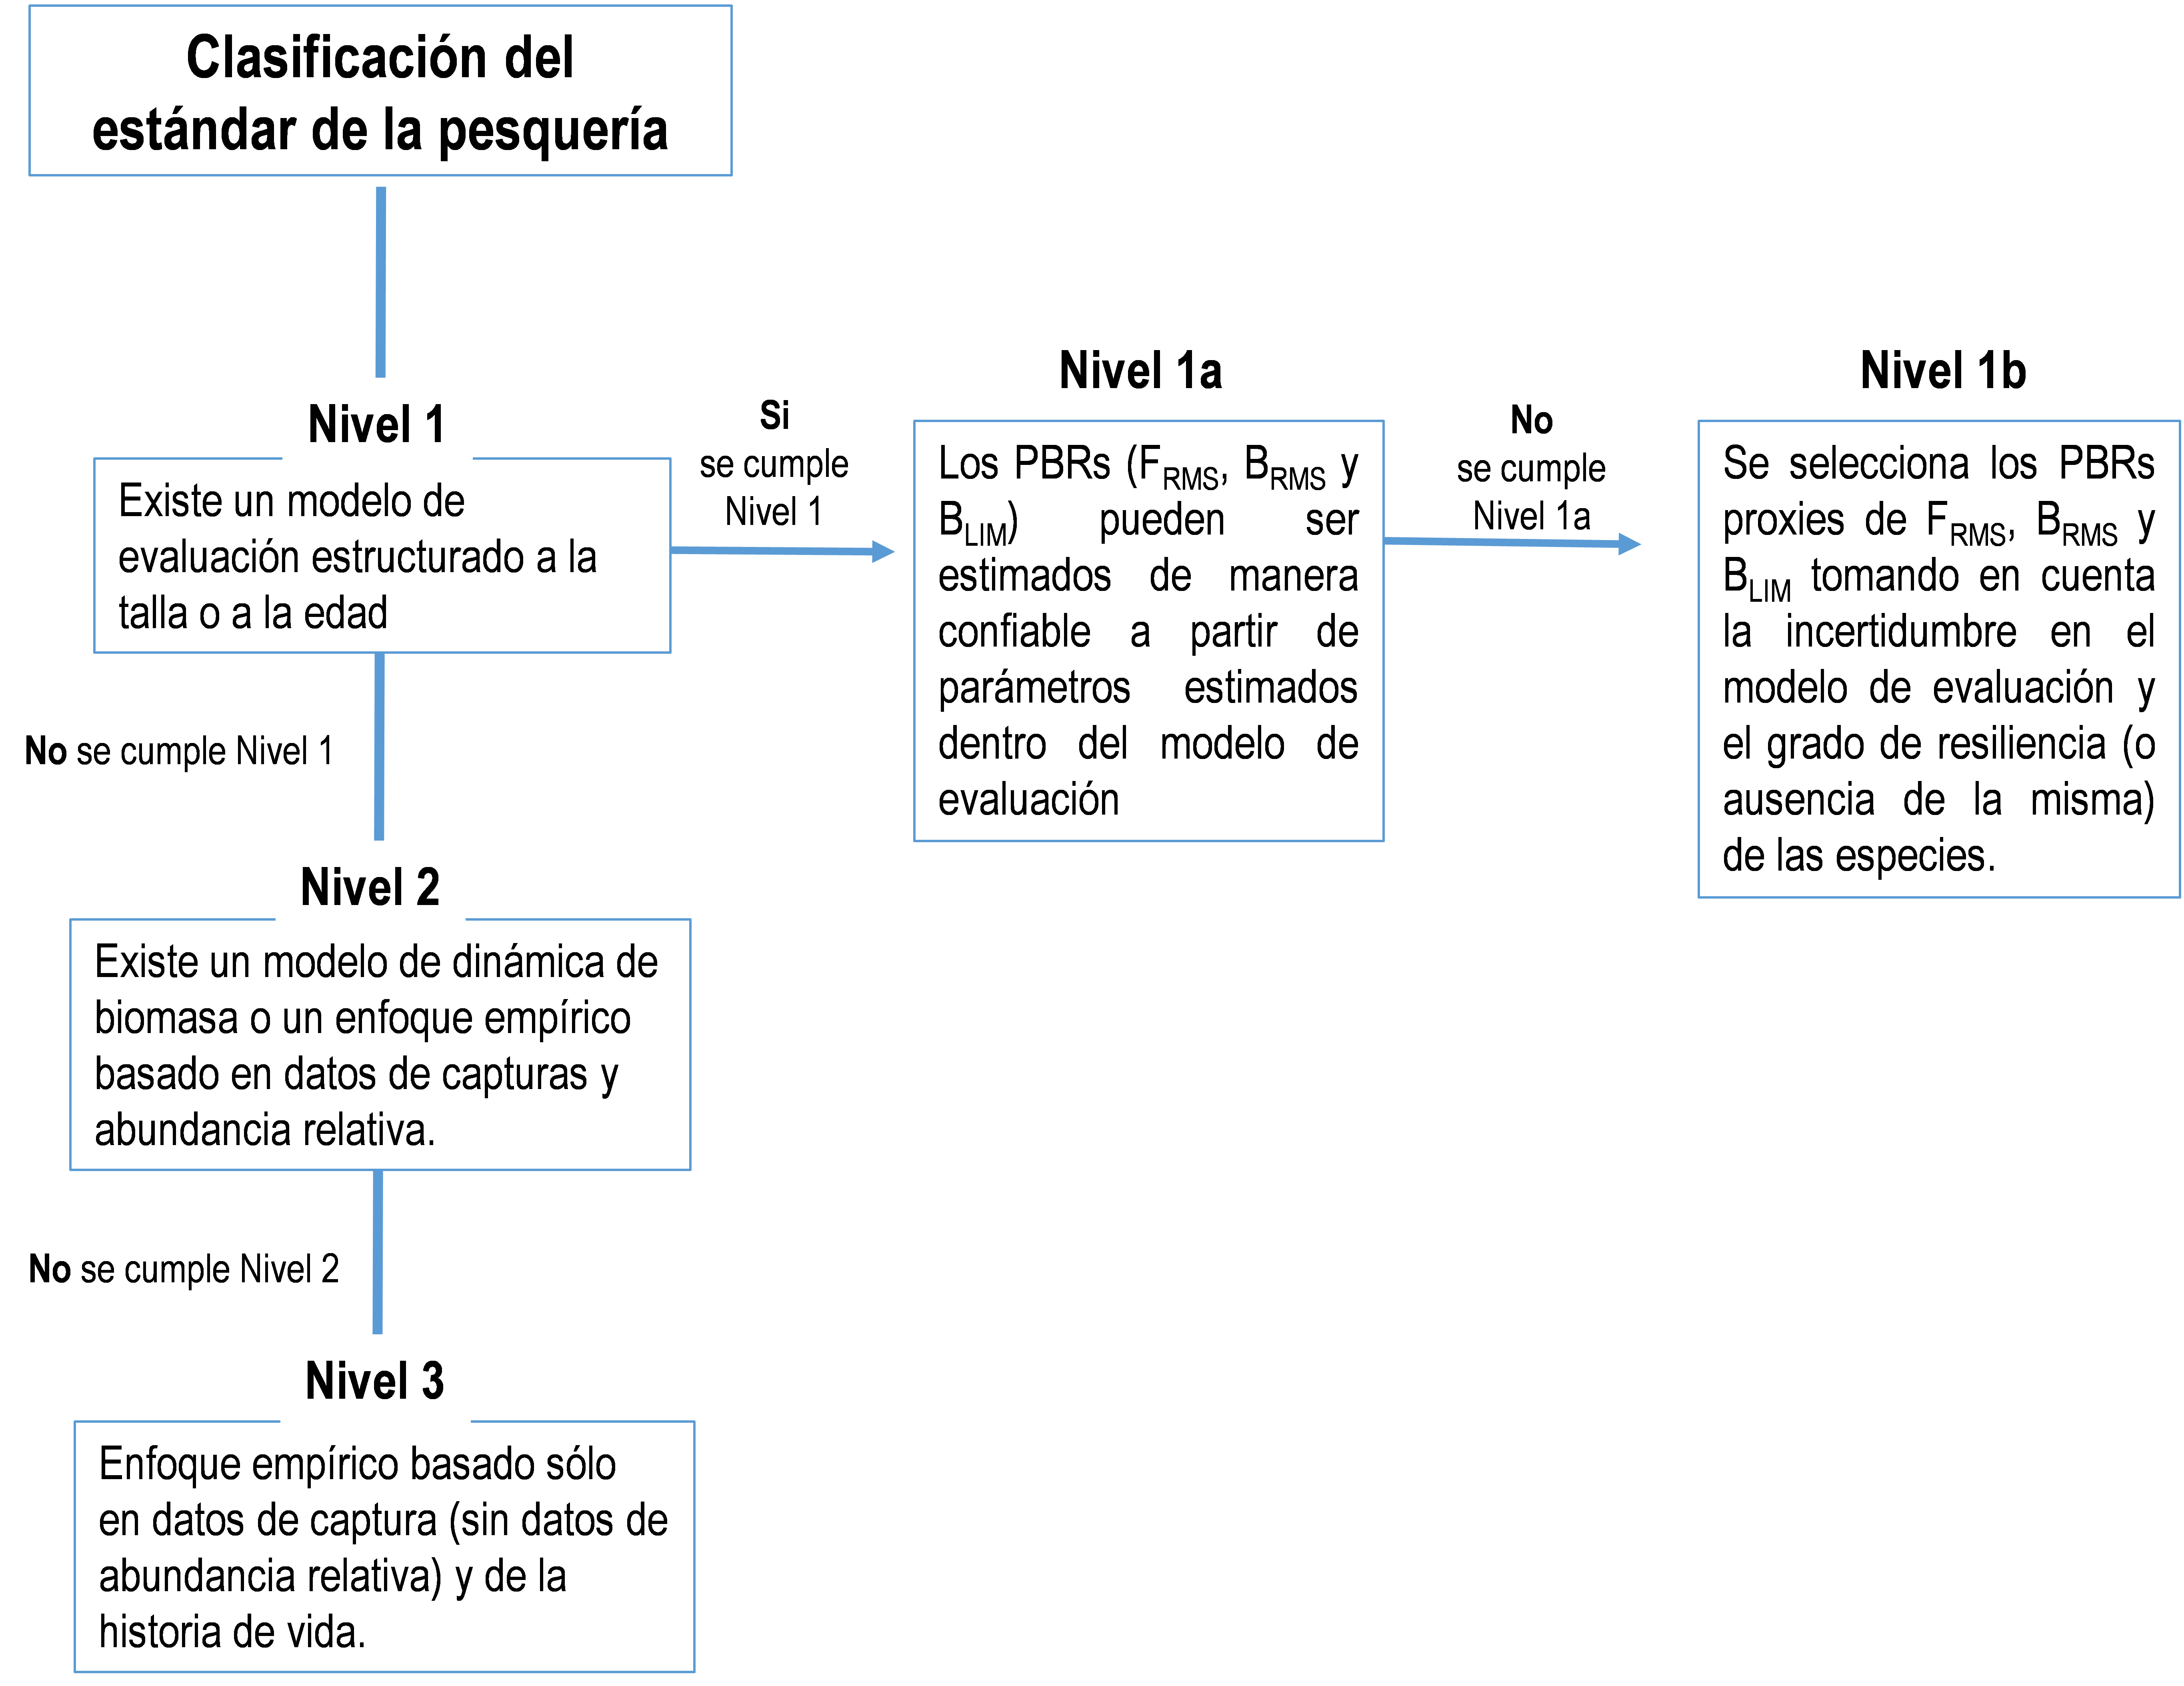
\includegraphics[width=1\textwidth]{FigurasInforme_Marzo/Figura12.png}
\end{center}

\small

\textbf{Figura 12}. Sistema de niveles para la determinación de los PBRs
de acuerdo a la cantidad, tipo y la calidad de la información disponible
y métodos de evaluación de stock empleados en cada pesquería.
\vspace{0.5cm} \normalsize

Al respecto, las anchovetas y sardinas son especies con una mortalidad
natural (M) alta (viven durante un período máximo de 4-5 años), crecen
rápido y maduran tempranamente. El reclutamiento está altamente
influenciado por el ambiente. El modelo de evaluación de stock tiene una
frecuencia temporal anual. Tanto el modelo y los datos son estructurados
a la edad. Se considera una flota comercial en el modelo de evaluación y
el patrón de selectividad es asumido constante a través de los años. El
modelo de evaluación de stock no incluye una relación S-R, sino
reclutamientos aleatorios. Estos antecedentes permiten clasificar a
anchoveta y sardina común centro-sur en el Tier 1b.

\hypertarget{datos-de-entrada-al-modelo-de-evaluaciuxf3n-de-stock}{%
\subsubsection{3.1.2. Datos de entrada al modelo de evaluación de
stock}\label{datos-de-entrada-al-modelo-de-evaluaciuxf3n-de-stock}}

A continuación, se detalla y fundamenta el conjunto de datos a emplear
para la estimación de los índices de abundancia, así como su forma de
utilización (ejemplo, indicadores absolutos o relativos). Además, se
informa la incertidumbre asociada a los indicadores de abundancia
propuestos para utilizar en la evaluación de sardina común.

\hypertarget{desembarques}{%
\paragraph{Desembarques:}\label{desembarques}}

Corresponde a la extracción registrada en puerto, independiente de la
zona de procedencia. Tiene valor en definir la importancia relativa de
los distintos puertos de descarga, por lo tanto, es de mayor interés
administrativo y/o comercial de la actividad. Su propósito es
cuantificar los volúmenes, totales y por especie, que efectivamente se
reciben en la descarga o desembarque. Las estadísticas oficiales de los
desembarques son sistematizadas por el Servicio Nacional de Pesca, sobre
una base mensual, por tipo de flota, puerto de desembarque y especie
objetivo. Cabe señalar que en la pesquería pelágica el concepto de
captura es igual al del desembarque más descarte. Para efecto de la
evaluación se utiliza la totalidad del desembarque por especie que
ocurre en la unidad de pesquería, comenzando la serie desde el año 1990
hasta 2020. La evaluación de stock es realizada en base al año biológico
(de julio a junio de cada año), y la serie de desembarques anuales es
convertida a temporada de pesca considerando la estacionalidad de la
pesquería y la serie oficial de desembarques anuales antes descrita.

\hypertarget{sobre-reportes}{%
\paragraph{Sobre-reportes:}\label{sobre-reportes}}

Existen algunos antecedentes que señalan que los desembarques del primer
semestre de los años 1999 y 2000 resultan ser muy altos para lo que en
ese entonces se supone era la población de anchoveta y sardina común.
Arcos \emph{et al}. (2004) postularon que las condiciones ambientales
pre El Niño y El Niño produjeron una alteración en la distribución
espacial de jurel, atrapando a los juveniles de la especie en la zona
centro-sur, generando la distorsión de los desembarques en los pequeños
pelágicos, impulsada por evadir multas y declarar menos jurel (Aranís,
2011). Basados en estos antecedentes, las series de desembarques anuales
oficiales fueron corregidos por investigadores de IFOP. Se realizó un
análisis preliminar utilizando la base de información de ``Muestreo de
Proporción de especies'' de IFOP, para comparar los datos de composición
de especies desembarcadas, la cual consiste en la selección de una
muestra de la captura de un contenedor (caja o balde), llenado en
distintos momentos del proceso de vaciado de la captura y luego se pesa
y cuenta la fauna diferenciada por especie. Posteriormente, se determina
la ``intencionalidad'' del viaje de pesca, basada en las proporciones de
captura, tomando el criterio de especie objetivo a la que representa más
del 50\% en peso de la muestra de proporción. En el caso de existir más
de dos especies, se considera como objetivo la de mayor contribución,
siendo clasificadas las restantes como fauna acompañante. Finalmente, se
obtiene la composición original para jurel, sardina y anchoveta
registrada de los desembarques, contrastado con las proporciones
re-estimadas obtenidas de los muestreos pelágicos que se practicaron en
ese período (1998-2001).

\hypertarget{sub-reportes}{%
\paragraph{Sub-reportes:}\label{sub-reportes}}

El año 2016 la Pontificia Universidad Católica de Chile desarrolló un
proyecto orientado a la corrección de las capturas totales históricas de
la pesquería de sardina común y anchoveta V-X Regiones (Proyecto CUI
2015-72-DAP-27) y recientemente IFOP realizó un estudio de remociones
totales en la flota artesanal que opera con red de cerco entre la Región
de Valparaíso y la Región de los Ríos orientando sus capturas a pequeños
pelágicos (Vega \emph{et al}. 2018). Para propósitos de la evaluación de
stock, esta información será analizada en el transcurso de este
proyecto, con el objeto definir la metodología a utilizar para la
corrección de las capturas y de este modo disminuir la incertidumbre
respecto al nivel real de captura de estos recursos.

\hypertarget{descarte}{%
\paragraph{Descarte:}\label{descarte}}

La pesquería de sardina común y anchoveta centro-sur es efectuada
mayoritariamente con cerco y destinada principalmente a la reducción,
por lo tanto, tendrían bajas tasas de descarte. Sin embargo, la
pesquería de carácter mixta de sardina común y anchoveta, junto con el
dispar estado de explotación de cada recurso y con establecimiento de
cuotas significativamente diferentes para cada uno, puede constituir un
fuerte incentivo en los usuarios para descartar el recurso limitante y
así poder completar la cuota de captura asignada al recurso principal.

Para abordar esta problemática, a partir del 2014 se desarrolló el
Programa de Observadores Científicos que estudió el descarte y captura
incidental de aves, mamíferos y tortugas marinas en las flotas cerqueras
artesanales e industrial de peces pelágicos de sardina común
(\emph{Strangomera bentincki}), anchoveta (\emph{Engraulis ringens}) y
jurel (\emph{Trachurus murphyi}) en la zona centro-sur, además de la
zona norte de Chile (XV a II regiones). El levantamiento de información
base para los análisis provino de la observación directa realizada a
bordo por observadores científicos, en complemento con información
entregada por los capitanes y patrones de pesca a través de una bitácora
de autorreporte. En las bitácoras los capitanes registran la información
de capturas totales por lance, los descartes, la pesca incidental y las
causas del descarte.

A partir de esta información, Vega \emph{et al}. (2017, 2018, 2019 y
2020) realizaron la estimación de captura total, estimación de descarte,
proporción de captura retenida y descartada, determinación de causas de
descarte, características biológicas de las especies objetivo y fauna
acompañante, junto a información de captura de pesca incidental y
mortalidad de aves, mamíferos y tortugas marinas en las flotas cerqueras
artesanales e industriales en las diferentes zonas de operación. La
estimación de capturas a bordo de embarcaciones cerqueras artesanales e
industriales, se realizó mediante la estimación del patrón o capitán de
pesca, a través de la lectura de equipos de detección, en conjunto con
una estimación visual en el fin del virado de la operación de pesca,
permitiendo la estimación del descarte, pues se realiza con la captura
en el agua.

El Artículo 7°B \footnote{\url{http://www.subpesca.cl/portal/616/articles-87217_documento.pdf}}
de la actual Ley General de Pesca y Acuicultura (LGPA, N° 18.892) indica
que no podrá realizarse el descarte de individuos de una especie
objetivo, cualquiera sea su régimen de acceso, y su fauna acompañante,
salvo que i) se haya fijado una cuota global anual de captura para la
especie objetivo y, ii) en el proceso de establecimiento de la cuota
global anual de captura se haya considerado el descarte.

En este sentido, Zúñiga \& Quiroz (2017) expusieron algunas opciones
para incorporar el descarte en el modelo de evaluación de stock, que
potencialmente representan fuentes de mortalidad por pesca a la fecha no
documentada. Estos escenarios fueron revisados por el CCT-PP en la
sesión de octubre 2017 (Acta 06/2017 \footnote{\url{http://www.subpesca.cl/portal/616/articles-98715_documento.pdf}})
donde fue seleccionado el escenario 5 que considera un 4\% de descarte
para el período 2000/01 - 2015/16 y un 2\% de descarte para los años
siguientes años. En el actual informe (septiembre 2020) se actualiza con
información del Programa de descarte 2019/20 (Vega \emph{et al}. 2020)
(\textbf{Tabla 3}).

\small
\begin{center} 
\textbf{Tabla 3.}
\end{center}
\begin{center} 
\vspace{-0.2cm} Estimaciones de captura total, retenida y descartada para sardina común en la zona centro-sur, para la pesquería industrial y artesanal año 2017, 2018 y 2019 (toneladas).  Datos de observador científico. A partir de la estimación de la proporción de especies en la captura. Fuente: Vega \textit{et al}. (2018, 2019 y 2020).
\end{center}
\vspace{-0.2cm}

\begin{table}[h]
    \centering
    \resizebox{15cm}{!} {
    \begin{tabular}{|c|l|l|c|c|c|c|}
    \hline
Año  &Flota       &Zona       &Captura Total &Captura Retenida &Captura Descartada &\% Descarte     \\ \hline
2017 &industrial  &centro-sur &14.068        &16.889           &178                &1\%             \\
2017 &artesanal   &Valparaíso &2.363         &2.334            &29                 &1\%             \\
2017 &artesanal   &Biobío     &172.048       &168.474          &3.574              &2\%             \\
2017 &artesanal   &Los Ríos   &41.119        &40.078           &1.041              &3\%             \\ \hline
2017 &Flota Total &Zona Total &\textbf{229.598} &\textbf{227.775} &\textbf{4.823}  &\textbf{2\%}    \\ \hline
2018 &industrial  &centro-sur &15.566        &12.689           &2.880              &19\%            \\
2018 &artesanal   &Valparaíso &5.962         &5.962            &0                  &0\%             \\
2018 &artesanal   &Biobío     &254.575       &235.546          &19.030             &7,5\%           \\
2018 &artesanal   &Los Lagos  &30.653        &29.792           &861                &2,8\%           \\ \hline
2018 &Flota Total &Zona Total &\textbf{306.756} &\textbf{283.986} &\textbf{22.771} &\textbf{7\%}    \\ \hline
2019 &industrial  &centro-sur &              &                 &                   &                \\
2019 &artesanal   &Valparaíso &              &                 &                   &                \\
2019 &artesanal   &Biobío     &120.381       &116.388          &3.993              &0,33\%          \\
2019 &artesanal   &Los Lagos  &50.188        &43.803           &6.385              &12,7\%          \\ \hline
2019 &Flota Total &Zona Total &\textbf{170.569} &\textbf{160.191}  &\textbf{10.378}&\textbf{6\%}    \\ \hline
  \end{tabular}}
        \end{table}

\normalsize

\hypertarget{seguimiento-de-la-pesqueruxeda}{%
\paragraph{Seguimiento de la
pesquería:}\label{seguimiento-de-la-pesqueruxeda}}

El monitoreo de la pesquería de sardina común entre las regiones de
Valparaíso y Los Lagos es realizado por el Proyecto de Investigación
Situación Pesquerías de Peces Pelágicos, que forma parte del Programa de
Seguimiento de las Principales Pesquerías Nacionales y es encargado por
la Subsecretaría de Pesca a IFOP. Este proyecto permite obtener
indicadores como las estructuras de edad/talla y peso medio a la edad,
entre otros:

\hypertarget{composiciuxf3n-por-edadtalla}{%
\subparagraph{Composición por
edad/talla:}\label{composiciuxf3n-por-edadtalla}}

Denominada también como estructura de edad, corresponde a la expansión
de la captura mediante la clave edad-talla determinada. Así esta
composición corresponde a la matriz que representa la distribución de
los ejemplares que están presentes en la captura, por grupo de edad y
por estrato de tamaño, a través de un diseño de muestreo de otolitos
estratificado por clase de tallas. A pesar de que se dispone de una
composición por zona, trimestre y flota, para efecto de la evaluación se
considera la estimación global para la unidad de pesquería y agregadas
entre flotas, estando disponible una serie construida desde el año 1990
hasta junio 2020. Esta información es empleada en el proceso de
evaluación de stock a objeto de evaluar los supuestos de la mortalidad
por pesca diferenciada por grupos de edad, además de entregar señales de
la fuerza de las clases anuales que han atravesado por la pesquería.

La estructura de tallas del desembarque o captura corresponde al número
de ejemplares, por rango de talla, capturados por la flota. En términos
generales, el diseño de muestreo asociado a la estructura de tallas del
desembarque corresponde a un diseño en dos etapas, donde la primera son
los viajes y la segunda los ejemplares. También y con menos frecuencia,
se lleva a cabo un muestreo en tres etapas, es decir, un muestreo dentro
de un viaje, lance y ejemplares. El indicador se obtiene por estratos de
zona y mes inicialmente, a través de la ponderación de la estructura de
talla con la captura diaria o temporal evaluada de las embarcaciones.

\hypertarget{pesos-a-la-edad}{%
\subparagraph{Pesos a la edad:}\label{pesos-a-la-edad}}

El crecimiento intra-anual de la sardina común es recogido en dos
matrices de pesos medios a la edad, las que corresponden respectivamente
a las estimaciones a mitad de año (enero) luego de la asignación de la
edad, y las estimaciones de pesos iniciales del año (julio) calculadas
en base a una media geométrica de la estimación actual y la del año
anterior rezagado en un año de edad. El peso medio (\(w_{(a,t)}^{med}\))
es empleado para generar las estimaciones de desembarques y la biomasa
del crucero de verano, mientras el peso inicial (\(w_{(a,t)}^{ini}\)) es
utilizado en las estimaciones de biomasa total, desovante y biomasa del
crucero de otoño. Dada la importancia de esta matriz de pesos medios
para la definición del estatus de sardina común se realiza una revisión
y corrección del método de estimación el cual es presentado como una
mejora al caso base de la actual evaluación que consiste en los
siguientes pasos.

Paso 1: Cálculo de pesos iniciales para el grupo de edad 0

\begin{center} 
$w_{(0,t)}^{ini}=exp(ln(w_{(a,t)}^{med} )-0.5*(ln(w_{(a+1,t+1)}^{med} )-ln(w_{(a,t)}^{med} )))$
\end{center}

Paso 2: Cálculo de pesos iniciales para grupos de edad 1 a 4

\begin{center} 
$w_{(a,t)}^{ini}=vw_{(a-1,t-1)}^{med}*w_{(a,t)}^{med}$
\end{center}

\hypertarget{cruceros-de-evaluaciuxf3n-hidroacuxfastica}{%
\paragraph{Cruceros de evaluación
hidroacústica:}\label{cruceros-de-evaluaciuxf3n-hidroacuxfastica}}

La historia de las evaluaciones hidroacústicas comenzó en la primavera
de 1995, estableciéndose un programa sistemático desde 1999 realizándose
cruceros de evaluación centrados en el periodo estival donde se maximiza
la presencia de juveniles. A partir del 2003 se replicó la prospección
en otoño para incrementar la certeza de la estimación haciendo un
seguimiento de la evolución del proceso, estudiándose además, las
asociaciones con las condiciones hidrográficas predominantes. De este
modo, ha sido posible establecer una estacionalidad en la composición
específica de las biomasas de estas dos especies, donde en verano la
sardina domina respecto a la anchoveta, mientras que en el otoño se
presenta un incremento relativo de la anchoveta y una reducción en la
sardina junto a cambios en su distribución geográfica (Castillo \emph{et
al}. 2013).

En este contexto, el presente proyecto considera los resultados de dos
cruceros de prospección, el primero a realizar en el verano (2000 -
2020), centrado en el máximo del reclutamiento (enero) y el segundo en
otoño (2003-2020), a fin de hacer un seguimiento del evento de verano o
capturar un eventual segundo pulso en el otoño (mayo), especialmente en
anchoveta. La zona de evaluación hidroacústica corresponde a la
delimitada entre los 33°50'S y 41°30'S en la cual se desarrolla la mayor
parte de la pesquería. En el área de estudio se realizan transectas
diurnas y replicas nocturnas y además, se realizan lances de pesca de
media agua y de cerco. La estimación de la abundancia por estructura de
talla se realiza en función de subzonas, las cuales son agrupadas de
acuerdo a la similitud en las estructuras de tallas observadas. Para
cada subzona, se agrupan los lances de pesca determinándose una
estructura de tallas común. Se obtiene el aporte en talla y
correspondiente peso, derivándose el TS y coeficiente de integración.

La estimación de la abundancia y biomasa de sardina común por subzona
queda determinada por el área prospectada en cada subzona, el
coeficiente de ecointegración a la talla y estimador de razón a la
talla. Este último se estima por tres métodos: Hansen \& Wolter,
Bootstrap, y Variables Regionalizadas. Para transformar la abundancia en
biomasa se utilizan los pesos medios a la talla obtenidos de la relación
longitud-peso. Las biomasas estimadas a través de los cruceros
hidroacústicos son empleadas en el proceso de evaluación de stock como
índices de abundancia poblacional (proporcionales a la biomasa) de
verano y otoño, respectivamente. La biomasa estimada por el modelo
corresponde a aquella fracción de la población sujeta a la selectividad
de los cruceros que son asumidos distintos entre verano y otoño, pero
constantes en el tiempo.

La Composición de edad/talla del crucero, denominada también como
estructura de edad, corresponde a la expansión de la abundancia mediante
la clave edad-talla determinada. A partir de la abundancia en número
estimada para cada talla en la evaluación hidroacústica, se expande la
abundancia por grupos de edad, haciendo uso de la clave talla edad la
cual obedece a la totalidad del área de estudio. La suma de la
abundancia por subzona por intervalo de talla, permite construir la
estimación total de abundancia para la zona de estudio. La estimación de
esta clave talla-edad obedece a un diseño de muestreo estratificado por
clase de tallas, dentro de las cuales es estimada una estructura de edad
por talla. La abundancia en número por grupo de edad se construye a
partir de la clave talla-edad anterior y la abundancia estimada por
intervalo de talla. Se obtienen entonces matrices completas las que
presentan explícitamente toda la estructura interna de la abundancia en
número de individuos por clase de longitud y para cada grupo de edad.

A partir de mayo de 2003, se han realizado evaluaciones acústicas de
ambos recursos a través de cruceros de otoño (PELACES). La estimación de
abundancia y biomasa por grupo de talla es similar al procedimiento del
crucero de verano. Sin embargo, algunos años de las evaluaciones
acústicas de otoño, no son muy consistentes en términos del área
cubierta y periodo del año en que se realizaban (mayo de 2003,
marzo-abril, mayo-junio de 2005 y mayo-junio de 2015), por lo tanto, los
cambios en abundancia de estos años podrían estar influenciadas por la
disponibilidad del recurso más que por cambios reales en abundancia. En
efecto, la época del año en que se realiza la prospección difiere entre
años, con desfase de un mes. Asimismo, las áreas prospectadas son
diferentes al crucero de verano, y el arte de pesca empleado en los
lances también difiere, siendo en este periodo solo captura de cerco.
Finalmente, no se dispone de lectura de edades para el periodo 2003 -
2006. De este modo, se realizó la eliminación de los datos de biomasa
acústicas del crucero de otoño correspondientes a los años 2003, 2005 y
2015, además de la estructura de edad del año 2015 por las razones antes
expuestas para el modelo base actual.

\hypertarget{paruxe1metros-de-historia-de-vida}{%
\paragraph{Parámetros de historia de
vida:}\label{paruxe1metros-de-historia-de-vida}}

Para la implementación del procedimiento de evaluación se recoge el
conocimiento de estudios científicos y técnicos que reportan información
asociada a los parámetros del ciclo vital de la especie, como la
mortalidad natural, el crecimiento y madurez, entre otros. De esta
forma, el proyecto tiene un rol de integración del conocimiento y
utiliza los productos de todos los programas y proyectos de
investigación para modelar la dinámica del recurso.

\hypertarget{evaluaciuxf3n-de-stock-1}{%
\subsubsection{3.1.3. Evaluación de
stock}\label{evaluaciuxf3n-de-stock-1}}

\hypertarget{descripciuxf3n-del-modelo-base}{%
\paragraph{Descripción del modelo
base:}\label{descripciuxf3n-del-modelo-base}}

El modelo de evaluación de stock de sardina común se basa en el análisis
estadístico de la dinámica de estructuras de edad anual y pesos medios a
la edad estimados del muestreo de tallas de los desembarques (período
1990 - junio 2020) y de los cruceros acústicos de verano (RECLAS, desde
2001 - 2020) y otoño (PELACES, período desde 2007 hasta 2020), de los
índices de biomasa de los cruceros acústicos (biomasa de reclutas en
verano, período desde 2000 hasta 2020 y biomasa vulnerable en otoño,
desde 2003 al 2020 y los desembarques totales (período 1990 - junio
2020), estos últimos convertidos a temporada de pesca considerando la
estacionalidad de la pesquería. Las fuentes de información utilizados en
la evaluación de sardina común se resumen en la \textbf{Tabla 4}.
Adicionalmente, en la \textbf{Sección 3.3.1.} de este informe se
detallan los datos y supuestos utilizados en las distintas etapas de
estimación de la CBA 2021.

La población de sardina común centro-sur constituye una unidad de stock
en la cual las variaciones se explican por capturas, reclutamientos,
mortalidad natural y por pesca, la información es agregada en año
biológico de manera que los cruceros de verano (enero) representan la
situación de la población a mitad del año y los de otoño, a la biomasa
poco antes del término del período anual (mayo). Por otra parte, el peso
a mitad del año biológico (peso medio) es empleado para generar las
estimaciones tanto del crucero de verano como de los desembarques,
mientras que el peso calculado a inicios del año biológico (inicios de
julio) representaría el peso de la biomasa desovante que ocurre en
agosto y los cruceros de otoño que ocurren en mayo (\textbf{Tabla 5}).
En la actualidad el método ha sido empleado bajo un enfoque en edades
agrupado en año biológico y que incorpora los siguientes elementos:

\begin{itemize}
\tightlist
\item
  Modelo de dinámica poblacional estructurada por edad (\textbf{Tabla
  6}),
\item
  Modelos de las observaciones y penalizaciones a priori que permiten
  relacionar el modelo de dinámica con las observaciones (\textbf{Tabla
  7}),
\item
  Identificación de la estructura del error a través de funciones de
  log-verosimilitud negativas (\textbf{Tabla 8}) y
\item
  Proceso de estimación de los parámetros desconocidos del modelo de
  dinámica a través de un algoritmo que minimiza la función objetivo
  total, contrastando las observaciones con las estimaciones deducidas
  del modelo de dinámica (\textbf{Tabla 9}).
\end{itemize}

\small
\begin{center} 
\textbf{Tabla 4.}
\end{center}
\begin{center} 
\vspace{-0.2cm} Resumen de los datos e información de entrada al modelo de evaluación de stock de sardina común.
\end{center}
\vspace{-0.2cm}

\begin{table}[h]
    \centering
    \resizebox{16cm}{!} {
    \begin{tabular}{|l|l|l|}
    \hline
Datos de entrada             & Período                            & Fuente de la información                \\ \hline
Desembarques totales anuales & Desde julio 1990- junio 1991       & Estadísticas oficiales de desembarques,  \\ 
                             & hasta el año biológico             & sistematizadas por el Servicio            \\ 
                             & julio 2019- junio 2020             & Nacional de Pesca.                         \\ \hline
\textbf{Composición de talla/edad} &                              &                                             \\
                             &                                    & \\
1. Flota                     & Desde julio 1990- junio 1991       & Monitoreo de la pesquería, de sardina común  \\
                             & hasta el año biológico             & de la V-X Regiones realizado por el           \\
                             & julio 2019- junio 2020             & Proyecto Investigación Situación Pesquerías    \\
                             &                                    & de Peces Pelágicos                              \\ 
2. Cruceros de verano        & Desde enero 2001 hasta enero 2021  &                                             \\
3. Cruceros de otoño         & Desde mayo 2007 hasta mayo 2020    & Evaluaciones hidroacústicas de los stocks    \\
                             &                                    & \\
\textbf{Biomasa acústica}    &                                    & de anchoveta y sardina común entre            \\
                             &                                    & \\
1. Cruceros de verano        & Desde enero del 2001               & la V y X regiones.                             \\
                             & hasta enero del 2021               &                                                 \\
2. Cruceros de otoño         & 2003,2005-2007,2009-2020           &                                                  \\ \hline
                             &                                    & \\
Pesos medios a la edad       & Desde julio 1990- junio 1991       & Monitoreo de la pesquería, de sardina común de la \\   
                             & hasta el año biológico             & V-X Regiones realizado por el Proyecto Investigación \\
                             & julio 2019- junio 2020             & Situación Pesquerías de Peces Pelágicos               \\ 
                             &                                    &                                                  \\ \hline
Madurez sexual a la edad     & Constante                          & Aranís \textit{et al}. (2005)                          \\ \hline
Mortalidad natural           & Constante                          & Cubillos \textit{et al}. (1998)                         \\ \hline 
  \end{tabular}}
        \end{table}

\pagebreak

\small
\begin{center} 
\textbf{Tabla 5.}
\end{center}
\begin{center} 
\vspace{-0.2cm} Resumen de los principales supuestos del modelo de evaluación anual con información a la edad (MAE) asociados a los datos observados.
\end{center}
\vspace{-0.2cm}

\begin{table}[h]
    \centering
    \resizebox{16cm}{!} {
    \begin{tabular}{|l|c|l|}
    \hline
 Datos observados              & Símbolo          & Supuestos                                                            \\ \hline
 Desembarque total anual       &$Y_t$             & Representa a la captura total del período anual julio-junio          \\ 
                               &                  & (año biológico). Se considera continua al interior del año biológico.\\
                               &                  & Desviación estándar supuesto como parte del error de observación     \\
                               &                  & $\sigma_f=0,01$                                                      \\ \hline
 Biomasa total del crucero de  &                  &                                                                      \\
 verano (RECLAS)               & $B_t^{cv}$       & Representa a la biomasa que ocurre a mitad del año biológico,        \\
                               &                  & ($dt^{cv}=0,5$ del año).Desviación estándar supuesto \\
                               &                  & como parte del error de observación  $\sigma_{cv}=0,3$.\\ \hline
Biomasa total del crucero de   &                  & Representa a la biomasa poco antes del término del período anual, (mayo), \\
otoño (PELACES)                & $B_t^{co}$       & ($dt^{co}=0,83$ del año). Desviación estándar supuesto \\
                               &                  & como parte del error de observación $\sigma_{co}=0,3$. \\ \hline
Proporción de la abundancia    &                  & \\
a la edad de la flota          & $p_{(a,t)}^f$    & Representa la distribución de los ejemplares que están presentes \\ 
                               &                  & en la captura total por grupo de edad. Tamaño de muestra efectivo \\
                               &                  & supuesto como parte del error de observación  $n^f=8$.\\ \hline
Proporción de la abundancia    &                  & \\
a la edad del Crucero verano   & $p_{(a,t)}^{cv}$   & Representa la distribución de los ejemplares que están presentes \\
                               &                  & en la captura del crucero de verano (enero) por grupo de edad. \\
                               &                  & Tamaño de muestra efectivo supuesto como parte del error de \\
                               &                  & observación $n^{cv}=9$.\\ \hline
Proporción de la abundancia    &                  & \\
a la edad del Crucero otoño    & $p_{(a,t)}^{co}$ & Representa la distribución de los ejemplares que están presentes \\
                               &                  & en la captura del crucero de otoño (mayo) por grupo de edad. \\
                               &                  & Tamaño de muestra efectivo supuesto como parte del error de \\
                               &                  & observación $n^{co}=7,5$. \\ \hline
Peso medio anual               & $w_{(a,t)}^{med}$& Es el peso medio empleado para generar estimaciones de biomasa \\
                               &                  & acústica de verano y desembarques. \\ \hline
Peso medio a inicios del año   & $w_{(a,t)}^{ini}$& Representa al Peso a inicios del año biológico (julio) \\
                               &                  & Empleado para generar estimaciones de biomasa total, biomasa \\
                               &                  & acústica de otoño y biomasa desovante. \\ \hline
  \end{tabular}}
        \end{table}

\pagebreak

\small
\begin{center} 
\textbf{Tabla 6.}
\end{center}
\begin{center} 
\vspace{-0.2cm} Dinámica básica del Modelo Anual con información en Edades (MAE).
\end{center}
\vspace{-0.2cm}

\begin{table}[h]
    \centering
    \resizebox{17cm}{!} {
    \begin{tabular}{|l|l|l|}
    \hline
Variable             &  Ecuación                                                           &    Descripción\\ \hline
Reclutamiento anual  & $N_{(a=0,t)}=R_0 e^{(\varepsilon_t+0,5\sigma_R^2)}$                 & El reclutamiento se asume a inicios de enero \\
                     &                                                                     & de cada año. \\ \hline
Población inicial    & $N_{(a=0,t=1)}=R_0e^{(-aM)}$                                        & $\varepsilon~N(0,\sigma_R^2 )$  \\
                     & $N_{(a>0,t=1)}=N_{(0,a>0)} e^{(\varepsilon_{(a>0)}+0,5\sigma_R^2)}$ & $lnR_0~U[a,b]$ \\ \hline
Abundancia           & $N_{(a,t)}=N_{(a-1,t-1)}$                                           &  $a$ es la edad y  \\
Sobrevivencia        & $S_{(a-1,t-1)}$ $S_{(a,t)}=exp(-Z_{(a,t)} )$                        &  $t$ es el año $a=[0,1,2,3,4]$ \\ \hline
Mortalidad total     & $Z_{(a,t)}=M+F_t s_a^f$                                             & $F_t$ es el efecto anual de la mortalidad \\
                     &                                                                     & por pesca. $F_t$ tiene variaciones estocásticas entre\\
                     &                                                                     & años y edades, pero estas quedan \\
                     &                                                                     & representadas por el patrón de selectividad \\
                     &                                                                     & edad-específica $s_a^f$ invariable entre años y la \\
                     &                                                                     & mortalidad por pesca anual $F_t$ La mortalidad natural \\
                     &                                                                     & es constante entre años y edades.\\ \hline
Selectividad de la   & $s_a^f=(1+exp[-ln19\frac{(a-A_{(50)}^f)}{\Delta^f}])^{-1}$          & $A_{(50)}^f$ edad al 50\% de la flota\\
flota                &                                                                     & $\Delta^f$ rango entre la edad al 95\% y 50\% \\ \hline
Biomasa total        & $B_t=\sum_a N_{(a,t)} w_{(a,t)}^{ini}$                              & $w_{(a,t)}^{ini}$ es el peso medio a la edad (a) \\
                     &                                                                     & y a inicios del año (t).\\ \hline
Biomasa desovante    & $BD_t=\sum_aN_{(a,t)} e^{(-dtZ_{(a,t)})} w_{(a,t)}^{ini}O_a$        & $dt$ es la fracción del año en la cual ocurre el \\
                     &                                                                     & desove ($dt =0,16$). \\
                     &                                                                     & $w_{(a,t)}^{ini}$ es el peso medio a la edad $a$ \\
                     &                                                                     & y a inicios del año $t$. $O_a$ es la ojiva de madurez sexual a la edad \\ \hline
  \end{tabular}}
        \end{table}

\pagebreak

\small
\begin{center} 
\textbf{Tabla 7.}
\end{center}
\begin{center} 
\vspace{-0.2cm} Modelo de las observaciones del Modelo Anual con información en Edades (MAE).
\end{center}
\vspace{-0.2cm}

\begin{table}[h]
    \centering
    \resizebox{17cm}{!} {
    \begin{tabular}{|l|l|l|}
    \hline
Variable                   &    Ecuación                                                           &    Descripción \\ \hline
Captura estimada en número &                                                                     & \\
a la edad                    & $\hat C_{a,t}=\frac{F_{a,t}}{Z_{a,t}}N_{a,t} (1-S_{a,t})$           & $\hat C_{a,t}$ captura en número estimada \\
                           &                                                                     & a la edad a y en el año t \\ \hline
Desembarques en peso       & $\hat Y_t= \sum_a \hat C_{a,t} w_{a,t}^{med}$                       & $w_{a,t}^{med}$ es el peso medio a la edad a y año t. \\ \hline
Proporción de la captura   &                                                                     & \\
a la edad de la flota      & $p_{a,t}^f=\frac{\hat C_{a,t}}{\sum_a C_{a,t}}$                     & $\hat C_{a,t}$ Captura en número estimada a la edad.\\ \hline
Abundancia a la edad       & $\hat N_{a,t}^{cv}=N_{a,t} e^{(-dt^{cv} Z_{a,t})} s_a^{cv}$         & $dt^{cv}$ es la fracción del año en la \\
disponible al crucero de   &                                                                     & cual se realiza el crucero de \\
verano                     &                                                                     & verano, ($dt^{cv}=0,5$, enero). \\ \hline
Selectividad del crucero   &                                                                     &\\
de verano                  & $s_a^{cv}=1+exp[-ln19((a-A_{50\%}^{cv})/dt^{cv}]^{(-1)}$            & $A_{50\%}^{cv}$ edad al 50\% \\
                           &                                                                     & $\Delta^{cv}$ rango entre la edad al 95\% y 50\% \\ \hline
Biomasa acústica total     &                                                                     &\\
del verano                 & $\hat B_t^{cv}=q^{cv} \sum_a \hat N_{a,t}^{cv} w_{a,t}^{med}$       & $w_{a,t}^{med}$ es el peso medio a la edad a y año t.\\
                           &                                                                     & $q^{cv}$ es la capturabilidad/ \\
                           &                                                                     & disponibilidad del crucero de verano.\\ \hline
Proporción de la abundancia&                                                                     & \\
la edad del crucero de     & $\hat p_{a,t}^{cv}=\frac{\hat N_{a,t}^{cv}}{\sum_a\hat N_{a,t}^{cv}}$& $\hat N_{a,t}^{cv}$ Abundancia estimada a la \\
verano                     &                                                                     & edad del crucero de verano \\ \hline
Abundancia a la edad       &                                                                     & \\
disponible al crucero de   & $N_{a,t}^{co}=N_{a,t} e^{(-dt^{co} Z_{a,t} )} s_a^{co}$             & $dt^{co}$ es la fracción del año en la \\
otoño                      &                                                                     & cual se realiza el crucero de \\
                           &                                                                     & otoño ($dt^{co}=0,83$, mayo) \\ \hline
Selectividad del crucero   & $s_a^{co}=1+exp[-ln19(a-A_{(50\%)}^{co})/dt^{co} ]^{(-1)}$          & $A_{50\%}^{co}$ edad al 50\% \\
de otoño                   &                                                                     & $dt^{co}$ rango entre la edad al 95\% y 50\% \\ \hline
Biomasa acústica total     & $\hat B_t^{co}=q^{co} \sum_a \hat N_{a,t}^{co} w_{a,t}^{ini}$       & $w_{a,t}^{ini}$ es el peso medio a la edad (a) \\
del otoño                  &                                                                     & y a inicios del año biológico (t).\\ 
                           &                                                                     & $q^{co}$ es la capturabilidad/ disponibilidad del \\
                           &                                                                     & crucero de otoño.\\ \hline
Proporción de la abundancia&                                                                     & \\
a la edad del crucero      & $\hat p_{a,t}^{co}=\frac{N_{a,t}^{co}}{\sum_a \hat N_{a,t}^{co}}$   & $\hat N_{a,t}^{co}$ Abundancia estimada a la \\
de otoño                   &                                                                     & edad del crucero de otoño.\\ \hline
  \end{tabular}}
        \end{table}

\pagebreak

\small
\begin{center} 
\textbf{Tabla 8.}
\end{center}
\begin{center} 
\vspace{-0.2cm} Modelo de los errores del Modelo Anual con información en Edades (MAE).
\end{center}
\vspace{-0.2cm}

\begin{table}[h]
    \centering
    \resizebox{17cm}{!} {
    \begin{tabular}{|l|l|l|l|}
    \hline
Variable                & Error       & Ecuación                                                                          & Descripción \\ \hline
Índice de abundancia  &             &                                                                                   & \\
crucero de verano       & Lognormal   & $-l(I^{cv})=\frac{1}{2\sigma_{cv}^2} \sum_t (ln \hat B_t^{cv}-lnB_t^{cv} )^2+cte$ & $\sigma_{cv}$ es la desviación estándar del \\
                      &             &                                                                                   & índice $I^{cv}$ en escala logarítmica. \\
Índice de abundancia  &             &                                                                                   & \\ \hline
crucero de otoño        & Lognormal   & $-l(I^{co})=\frac{1}{2\sigma_{co}^2} \sum_t (ln \hat B_t^{co}-lnB_t^{co} )^2+cte$ & $\sigma_{co}$ es la desviación estándar del \\
                      &             &                                                                                   & índice $I^{co}$ en escala logarítmica. \\ \hline
Desembarque             & Lognormal   & $-l(Y)=\frac{1}{2\sigma_{f}^2} \sum_t (ln \hat Y_t-lnY_t )^2+cte$                 & $\sigma_{f}$ es la desviación estándar del \\
                      &             &                                                                                   & índice $Y$ en escala logarítmica.\\
Proporción de la      &             &                                                                                   & \\ \hline
captura a la edad de  & Multinomial &   $-l(p^f )=n^f p_{a,t}^f  ln \hat p_{a,t}^f$                                       & $p_{a,t}^f$ corresponde a la captura a la \\
la flota              &             &                                                                                   & edad de la flota. $n^f$ es el tamaño de \\
                      &             &                                                                                   & muestra efectivo.\\ \hline
Proporción de la      &             &                                                                                   & \\
abundancia a la       & Multinomial &   $-l(p^{cv} )=n^{cv} p_{a,t}^{cv}  ln \hat p_{a,t}^{cv}$                           & $p_{a,t}^{cv}$ corresponde a la captura a la \\
edad del crucero de   &             &                                                                                   & edad del crucero de verano. $n^{cv}$ es el \\
verano                &             &                                                                                   & tamaño de muestra efectivo.\\ \hline
Proporción de la      &             &                                                                                   & \\
abundancia a la       & Multinomial &   $-l(p^{co} )=n^{co} p_{a,t}^{co}  ln \hat p_{a,t}^{co}$                           & $p_{a,t}^{co}$ corresponde a la captura a la \\
edad del crucero de   &             &                                                                                   & edad del crucero de otoño. $n^{co}$ es el \\
otoño                 &             &                                                                                   & tamaño de muestra efectivo.\\ \hline
Prior                 &             &                                                                                   & \\ \hline
Desvíos del           &             &                                                                                   & \\
reclutamiento           & Lognormal   & $-l(R)=\frac{1}{2\sigma_R^2} \sum_t \varepsilon_t^2 +cte$                           & $\varepsilon_t$ desvíos del reclutamiento\\
                      &             &                                                                                   & $\sigma_R$ es la desviación estándar de los \\
                      &             &                                                                                   & reclutamientos \\ \hline
Capturabilidad de     &             &                                                                                   & \\
los cruceros            & Lognormal   & $-(q^{cv})=\frac{1}{2 \sigma_{q^{cv}}^2} ln(q^{cv})^2+cte$                        & $\sigma_q^{cv}$ es la desviación estándar de la \\  
                      &             & $-(q^{co})=\frac{1}{2\sigma_{q^{co}}^2} ln(q^{co})^2+cte$                         & capturabilidad del crucero de verano.\\
                      &             &                                                                                   & $\sigma_q^{co}$ es la desviación estándar de la    \\
                      &             &                                                                                   & capturabilidad del crucero de otoño.\\ \hline
Mortalidad por pesca  & Lognormal     & $-l(F_{1991,1992})=1000*((logF_{1991}-\bar F)^2+(logF_{1992}-\bar F)^2)$          & En esos años hubo estimaciones\\
                      &             &                                                                                   & muy bajas de reclutamiento y del \\
                      &             &                                                                                   & stock desovante asociados con \\
                      &             &                                                                                   & estos altos niveles de F1991,1992,\\ 
                      &             &                                                                                   & producto de que para esos años\\
                      &             &                                                                                   & existe poca información a parte de la\\ 
                      &             &                                                                                   & estructura de edad para la captura. \\
                      &             &                                                                                   & Por lo tanto, para corregir estos niveles\\ 
                      &             &                                                                                   & de F se le agrega una penalización a la \\
                      &             &                                                                                   & función objetivo\\ \hline
\multicolumn{2}{|l|}{Función objetivo} &\multicolumn{2}{|l|}{$-l(I^{cv} )-l(I^{co} )-l(Y)-l(p^f )-l(p^{cv} )-l(p^{co})-l(R)-l(q^{cv} )-l(q^{co} )-l(F_{1991,1992})$}\\ \hline
        \end{tabular}}
        \end{table}

\pagebreak

\small
\begin{center} 
\textbf{Tabla 9.}
\end{center}
\begin{center} 
\vspace{-0.2cm} Parámetros y prioris empleadas en el Modelo Anual con información en Edades (MAE).
\end{center}
\vspace{-0.2cm}

\begin{table}[h]
    \centering
    \resizebox{17cm}{!} {
    \begin{tabular}{|l|c|l|l|}
    \hline
Parámetro                                 & N de       & Prior                                            & Descripción \\ 
                                          & parámetros &                                                  &             \\ \hline
                                          &            &                                                  & \\
Mortalidad natural                        & 1          & $M=1,0$ (fijo)                                   & La mortalidad natural se \\
                                          &            &                                                  & asume constante entre años \\
                                          &            &                                                  & y edades. \\
                                          &            &                                                  & \\\hline
Mortalidad por pesca                      & 31         & $lnF \sim U[-6;1,6]$                             & $F_t$ representa el efecto anual \\
                                          &            &                                                  & de la mortalidad por pesca. \\
                                          &            &                                                  & \\ \hline
Selectividad de la flota                  &  2         & $lnA_{50\%}^f \sim U[-1;2]$                      & \\
                                          &            & $ln\Delta^f \sim U[-4;0,6]$                      & Se asume el patrón de \\
Selectividad de los cruceros de verano    &  2         & $lnA_{50\%}^{cv} \sim U[-1;2]$                   & selectividad $S_a^{f,cv,co}$\\
                                          &            & $ln\Delta^{cv} \sim U[-4;0,6]$                   & edad específica invariable  \\
Selectividad de los cruceros de otoño     &  2         & $lnA_{50\%}^{co} \sim U[-1;2]$                   & entre años \\
                                          &            & $ln\Delta^{co} \sim U[-4;0,6]$                   & \\ \hline   
                                          &            &                                                  & $R_0$ corresponde al \\
Reclutamiento promedio                    &  1         & $lnR_{0} \sim U[5;20]$                           & reclutamiento medio, el cual\\
                                          &            &                                                  & es considerado un parámetro\\
                                          &            &                                                  & desconocido a estimar, el que\\
                                          &            &                                                  & es multiplicado por una \\
                                          &            &                                                  & perturbación anual $\varepsilon_t$\\
                                          &            &                                                  & Adicionalmente, en la sección \\
                                          &            &                                                  & parámetros del código en ADMB se \\
Desvíos de reclutamiento $\varepsilon_t$  &  31        & $ln \varepsilon_t \sim N[0;\sigma_R^2]$          & consideran initboundedvector \\
Estructura etaria inicial $\varepsilon_t$ &  5         & $ln \varepsilon_a \sim N[0;\sigma_R^2]$          & logdesvNo(1,nedades-1,10,10,optdevNo)\\
                                          &            &                                                  & initboundeddevvector \\
                                          &            &                                                  & logdesvRt(1,nanos,-10,10,optdevR)\\
                                          &            &                                                  & \\\hline
                                          &            & $ln q^{cv} \sim N[0;\sigma_{q^{cv}}^2]$ (verano) &  La capturabilidad del crucero \\
Capturabilidad de los cruceros            &  2         & $ln q^{co} \sim N[0;\sigma_{q^{co}}^2]$ (otoño)  &  de otoño y verano es un parámetro\\
Desviación estándar de los desvíos de     &            & $\sigma_R = 0,6$                                 & que puede ser estimado libremente\\
reclutamientos, estructura etaria inicial &            & $\sigma_{q^{cv}} = 100.2 (verano)$                & por el modelo\\
y capturabilidad de cruceros              &            & $\sigma_{q^{co}} = 100.6 (otoño)$                 &\\ 
                                          &            &                                                  & \\ \hline
  \end{tabular}}
        \end{table}

\normalsize

\textbf{Tamaños de muestra}

De manera similar a los coeficientes de variación empleados para
ponderar los índices de abundancia y desembarques entre sus estimadores
de verosimilitud, el tamaño de muestra corresponde a una expresión
proporcional a la incertidumbre que tienen las composiciones de
tallas/edades de las capturas empleadas en la evaluación de stock.

De acuerdo a Francis (2011), los datos de composición de edad
corresponderían a medidas indirectas de la escala poblacional ya que
requiere conocer los mecanismos de selección de la pesquería y la
estructura por edades de la población. Por lo tanto, son mucho menos
informativos acerca del tamaño de la población y requiere supuestos
fuertes para obtener esa información. A pesar de lo anterior, los datos
de composición a la edad a menudo son más informativos que los índices
de abundancia. Por lo tanto, es importante asegurarnos que la dinámica
de la población esté influenciada por los datos más confiables. Un
factor relevante es el ponderador asociado con las composiciones de
edades de la flota y los cruceros acústicos de verano y otoño. Estos
ponderadores son asociados con el tamaño de muestra efectivo dado que la
función de probabilidad empleada es multinomial.

En la asesoría realizada en marzo de 2017 (Zúñiga, 2017), se estimó un
tamaño de muestra considerando las recomendaciones emanadas del workshop
sobre ponderadores de las fuentes de información en evaluación de stock,
realizados por Center for the Advancement of Population Assessment
Methodology (CAPAM, 2015:
\url{https://www.nwfsc.noaa.Gov/news/features/data_source_workshop}). Se
compararon dos metodologías para estimar el tamaño de muestra para la
flota y cruceros de verano y otoño, el método T.A 1.8, indicada por
Francis (2011) y el proceso iterativo recomendado por McAllister \&
Ianelli (1997) considerándose el promedio armónico (\textbf{Tabla 10}).

Ambos procesos inician con un valor arbitrario de tamaños de muestra,
comenzando con el valor empleado por defecto de la asesoría de
septiembre 2016 (Canales \& Zúñiga, 2016), nm=38 para la flota y nm=10
para el crucero de verano y nm=7,8 para el crucero de otoño, para luego
de repetidos ajustes del modelo, llegar a valores estables que son los
propuestos en esta evaluación de stock. A menudo es deseable verificar
estas estimaciones cuando en el modelo se van integrando nuevas
composiciones de edades/tallas o como estos valores pueden variar
dependiendo de cambios en los supuestos del modelo.

\small
\begin{center} 
\textbf{Tabla 10.}
\end{center}
\begin{center} 
\vspace{-0.2cm} Estimadores de tamaños de muestra empleados en el análisis.
\end{center}
\vspace{-0.2cm}

\begin{table}[h]
    \centering
    \resizebox{12cm}{!} {
    \begin{tabular}{|l|c|}
    \hline
    Fuente                                             &    Estimador \\ \hline 
                                                       & \\
    McAllister \& Ianelli (1997), donde $p_a$ es la     &   $\frac{\sum_a \hat{p}_{(y,a)} (1-\hat{p}_{(y,a)})}{\sum_a(p_{(y,a)}-\hat{p}_{(y,a)})^2 }$ \\ 
    proporción de la captura a la edad                 &                                                                                             \\ \hline
    Francis (2011), donde n1 es el tamaño de muestra   &    \\
    inicial, O y E corresponden a la edad (a) promedio & $n_1 var[\frac{(\bar{O}_y-\bar{E}_y )}{(\frac{\sum_a a^2 \hat{p}_{(y,a)}-\bar{E}_y^2}{n_1})^{0.5}}]^{-1}$ \\ 
    observada y estimada (TA 1,8)                      & \\ \hline
    \end{tabular}}
        \end{table}

\normalsize

\textbf{Coeficiente de variación}

Son empleados en los distintos índices de abundancia y capturas, miden
el nivel de desviación que el analista supone tienen los datos respecto
del valor central verdadero como parte del error de observación. El
coeficiente de variación tiene relevancia en las estimaciones pues es
inversamente proporcional con el peso que tiene una determinada fuente
de datos en la verosimilitud total.

Comúnmente se asignan bajos niveles de incertidumbre a los desembarques
y mayores a los cruceros, esto por el hecho que los desembarques son
mediciones directamente asociadas con la mortalidad por pesca, mientras
las estimaciones de biomasa de cruceros están sujetos a variados
criterios y consideraciones en sus estimaciones de una población ``no
observable'', lo que en definitiva insta a suponer que ellos tienen
mayor incertidumbre y/o son tratados como medidas relativas de
abundancia.

Al respecto, el peso relativo designado a la estimación de captura total
al ajustar el modelo de evaluación fue debatido durante el taller de
revisión por pares de sardina común, donde se consideró que la
limitación sobre los F efectivamente utilizada fue débil (CV=10\%). Se
sugiere un CV =1\% asumiendo que las capturas son conocidas exactamente
(\textbf{Tabla 5}). Esto se justifica debido a que existe poca o ninguna
información en los datos y estructura del modelo para estimar la captura
total, el modelo se ajusta asumiendo que las capturas se conocen
exactamente o con altos niveles de precisión. Bajo este supuesto, las
estimaciones de abundancia ``N'' del modelo y los parámetros de
separabilidad permitirían determinar F anual. Sin embargo, para la
ecuación de Baranov, no existe una solución analítica para los valores
de F, por lo tanto, se deben tratar como parámetros estimables, pero
altamente limitados (CV bajos) de tal manera que las capturas totales se
puedan estimar de manera muy precisa.

En relación a las biomasas estimadas en los cruceros acústicos y
cruceros de huevos, Francis (2011) propone la idea de aproximarse de
manera gradual a una medida del error, comenzando con un suavizador de
los datos, es decir, un análisis exploratorio que considere aquel
coeficiente de variación teórico que resulta de aplicar el ``mejor''
modelo de tendencia central a los datos aislados. Este primer
procedimiento no depende del modelo de evaluación de stock sino de la
variabilidad de los datos. Este procedimiento fue aplicado a las
biomasas estimadas en los cruceros acústicos y cruceros de huevos. Se
ajustó polinomios locales propuesto por Cleveland (1992), mediante la
función ``loess'' del paquete ``modreg'' en R Project. La estimación de
la tendencia central de los cruceros generó valores de CV=0,73 para el
crucero de verano y un CV=0,53 para el crucero de otoño.

En la revisión por pares de sardina se cuestionó este análisis,
señalando que el supuesto en que se basa este enfoque es razonable para
especies de larga vida donde el índice de abundancia está integrado a
través de un número de cohortes. El alto CV estimado para el crucero de
verano es producto principalmente de que las abundancias medidas son
dominadas por los reclutamientos más recientes que son altamente
variables. Además, considerar CVs tan altos evitaría su uso como índice
de abundancia en la evaluación. Los CVs (estadísticos) estimados para
los cruceros acústicos de verano y otoño en base a los estimados de
varianza de biomasa por talla y zona reportados en los informes
acústicos se encuentran en el orden de 15-20\% (\textbf{Tabla 11}). Sin
embargo, el modelo base actual asume un CV = 0,3 para los cruceros
acústicos de verano y otoño (\textbf{Tabla 5}).

\small
\begin{center} 
\textbf{Tabla 11.}
\end{center}
\begin{center} 
\vspace{-0.2cm} Estimaciones de las biomasas acústicas de verano y otoño y los CVs estadísticos estimados en cada uno de ellos.
\end{center}
\vspace{-0.2cm}

\begin{longtable}[]{@{}lllll@{}}
\toprule
Años & C. Verano (t) & CV \% & C. Otoño (t) & CV \%\tabularnewline
\midrule
\endhead
2000 & 252.601 & - & 0 & -\tabularnewline
2001 & 567.819 & 16 & 0 & -\tabularnewline
2002 & 844.713 & 16 & 0 & -\tabularnewline
2003 & 477.998 & 16 & 173.520 & -\tabularnewline
2004 & 351.125 & 12 & 0 & -\tabularnewline
2005 & 339.783 & 15 & 1.456.880 & -\tabularnewline
2006 & 2.178.397 & 8 & 552.880 & -\tabularnewline
2007 & 2.134.042 & 14 & 188.675 & 13\tabularnewline
2008 & 4.813.140 & 14 & 0 & -\tabularnewline
2009 & 1.555.620 & 20 & 991.730 & 11\tabularnewline
2010 & 2.623.565 & 7 & 2.467.720 & 17\tabularnewline
2011 & 3.216.857 & 11 & 1.416.034 & 29\tabularnewline
2012 & 3.843.000 & 15 & 1.217.170 & 12\tabularnewline
2013 & 1.133.480 & 10 & 2.296.490 & 20\tabularnewline
2014 & 3.079.434 & 6 & 1.805.815 & 12\tabularnewline
2015 & 1.972.148 & 21 & 2.440.448 & 25\tabularnewline
2016 & 2.032.684 & 5 & 1.482.799 & 10\tabularnewline
2017 & 2.025.002 & 15 & 1.565.315 & 17\tabularnewline
2018 & 2.424.330 & 13 & 1.577.507 & 7\tabularnewline
2019 & 2.275.425 & 5 & 1.421.176 & 8\tabularnewline
2020 & 1.050.175 & 7 & 867.257 & 4\tabularnewline
2021 & 2.363.380 & 4 & - & -\tabularnewline
\bottomrule
\end{longtable}

\normalsize

\hypertarget{penalizaciones}{%
\subparagraph{Penalizaciones:}\label{penalizaciones}}

Con el objeto de obtener valores biológicamente aceptables, a menudo se
emplean penalizaciones a ciertas estimaciones o parámetros. En el modelo
de evaluación empleado hasta febrero de 2014, las estimaciones de las
tasas de mortalidad por pesca en 1991 y 1992 son muy altas. El revisor
de RPP señala que dichas estimaciones altas parecen ser incoherentes con
la información disponible de la pesquería. En esos años hubo
estimaciones muy bajas de reclutamiento y del stock desovante asociados
con estos altos niveles de F, producto de que para esos años existe poca
información aparte de la estructura de edad para la captura. Por lo
tanto, para corregir estos niveles de F se le agrega una penalización a
la función objetivo.

\hypertarget{selectividad}{%
\subparagraph{Selectividad:}\label{selectividad}}

El patrón de explotación de la flota es asintótico y se considera
constante entre años tanto a nivel de parámetros de posición (edad al
50\% de explotación) como de dispersión (pendiente de la curvatura). Las
justificaciones para este escenario se basan en la poca variabilidad que
presentan las composiciones de edades de las capturas y en menor grado
en los cruceros, como también a que en esta pesquería no se conocen
procesos de escape significativos de individuos longevos fuera de la
zona donde opera la pesquería. En el caso de los cruceros de verano y
otoño, el patrón de explotación se supone igualmente logístico, pero se
estiman independientemente de la flota.

\hypertarget{capturabilidad-de-los-cruceros}{%
\subparagraph{Capturabilidad de los
cruceros:}\label{capturabilidad-de-los-cruceros}}

Se asume que tanto el crucero de verano como otoño representan una
fracción de la biomasa disponible, lo que en otras palabras se traduce
en que el índice de proporcionalidad o capturabilidad es estimado en el
modelo sujeto a una distribución a priori, establecida sólo respecto del
crucero de verano siguiendo una distribución lognormal con media 0 y
error estándar 0,2. Lo anterior se justifica dado que el reclutamiento
de la sardina común es menos extendido en el tiempo respecto de la
anchoveta y se puede medir en un solo crucero, de manera que el crucero
de verano reflejaría de mejor forma los niveles de la población dejando
el crucero de otoño como índice relativo de los cambios en la fracción
disponible para la flota (Castillo \emph{com. pers.}).

Al respecto, en el taller de Revisión Por Pares (RPP) se discutió sobre
los problemas asociados con la corrección de orilla, la composición de
especies, frecuencia de tallas, cardúmenes no detectados y corrección de
superficie y costa, etc, de los cruceros acústicos. Existe la
posibilidad de dar lugar a estimaciones considerablemente menores o
mayores que la abundancia real del recurso. En base a esto, Polacheck
(2014), señala que no existe una razón a priori para asumir que ``q'' en
un crucero debería ser más cercano a 1 que en el otro, ni que ``q'' para
cualquiera de los cruceros es cercano a 1. Se sugiere asumir un prior no
informativo como elección más apropiada para un caso base. De esta
forma, en el modelo actual, la capturabilidad de los cruceros acústicos
se asume con una distribución a priori lognormal con media 0 y error
estándar 100, es decir, se remueve el efecto de esta distribución a
priori.

\hypertarget{diagnuxf3stico-del-modelo-de-evaluaciuxf3n-de-stock}{%
\paragraph{Diagnóstico del modelo de evaluación de
stock}\label{diagnuxf3stico-del-modelo-de-evaluaciuxf3n-de-stock}}

\hypertarget{ajuste-del-modelo-a-los-datos}{%
\subparagraph{Ajuste del modelo a los
datos:}\label{ajuste-del-modelo-a-los-datos}}

Corresponde a la presentación gráfica del ajuste del modelo a los datos
observados y bondad de ajuste mediante diagrama QQ que permitirá evaluar
si los valores estimados se apartan significativamente del supuesto
inicial, esto es, que las observaciones con una muestra aleatoria de una
distribución log-normal con media y varianza conocida. Si los datos se
aproximan significativamente a la relación lineal implica entonces que
el supuesto es adecuado para los datos analizados.

\hypertarget{anuxe1lisis-de-residuos}{%
\subparagraph{Análisis de residuos:}\label{anuxe1lisis-de-residuos}}

Se entregará los residuales frente a los valores predichos para ver si
la varianza residual es constante, los residuales del modelo frente a
las variables explicativas (año) para determinar si la varianza es
homogénea entre los años, un histograma de los residuos para ver si hay
normalidad y un diagrama qqplot de los residuos que indica linealidad.

\hypertarget{comparaciuxf3n-con-evaluaciones-anteriores}{%
\subparagraph{Comparación con evaluaciones
anteriores:}\label{comparaciuxf3n-con-evaluaciones-anteriores}}

Se incluirá la comparación de resultados con versiones anteriores u
otros modelos para evaluar la consistencia de la evaluación presente
(análisis retrospectivo empírico). Sobre la base de estos análisis, se
identificarán las oportunidades de mejoras en la implementación del
procedimiento de evaluación, los vacíos de conocimiento y de
información, entre otros.

\hypertarget{anuxe1lisis-retrospectivo}{%
\subparagraph{Análisis retrospectivo:}\label{anuxe1lisis-retrospectivo}}

El análisis retrospectivo es otro diagnóstico que implica correr el
modelo eliminando años de datos sucesivos consecutivamente para estimar
el sesgo del modelo (Cadrin \& Vaughn 1997, Cadigan \& Farrell 2005). Se
realizó un análisis retrospectivo para probar la consistencia de cada
escenario de sensibilidad antes señalado. Este análisis permitirá
evaluar la robustez de cada escenario frente a nuevas piezas de
información lo que también permitirá validar el escenario ``caso base''.
Este análisis consiste en una validación cruzada de naturaleza
sistemática en la que es removido secuencialmente el último año de
información y se evalúa su impacto en las tendencias poblacionales. Este
análisis permite determinar si hubo un patrón consistente de
sobreestimación o subestimación en años sucesivos de la biomasa
desovante y mortalidad por pesca utilizados en la determinación del
estatus de sardina común.

Estadístico Rho: El estadístico rho de Mohn (1999) se ha utilizado
comúnmente para medir el patrón retrospectivo. Corresponde a la suma de
la diferencia relativa entre los valores de la serie de tiempo reducida
estimada por el modelo y los mismos valores estimados de la serie de
tiempo completa.

\vspace{0.5cm}
\Large
\begin{center} 
$\rho=\sum_{y=1}^{npeels}\frac{X_{(Y-y,tip)}-X_{(Y-y,ref)}}{X_{(Y-y,ref)}}$ 
\end{center}
\vspace{0.5cm}

\normalsize

Donde \(X\) corresponde a alguna variable de la evaluación de stock,
tales como BD o F, ``\(y\)'' corresponde a los años, ``\(npeels\)'' es
el número de años que son disminuidos de manera sucesiva, ``\(Y\)'' es
el último año de la serie de tiempo completa, ``\(tip\)'' es la
estimación terminal de la serie de tiempo reducida y ``\(ref\)'' es la
serie de tiempo completa.

Este cálculo será cero cuando la serie de tiempo reducida se encuentre
exactamente con la serie de tiempo completa, o cuando las diferencias
entre la serie disminuida y la serie completa están en equilibrio tanto
positivo como negativo. El rho de Mohn será grande, ya sea positivo o
negativo, cuando hay un patrón consistente de cambio en la serie de
tiempo reducida respecto a la serie completa.

\hypertarget{perfiles-de-verosimilitud}{%
\subparagraph{Perfiles de
verosimilitud:}\label{perfiles-de-verosimilitud}}

Algunos autores señalan que uno de los mejores diagnósticos para evaluar
la influencia de los datos en la dinámica estimada por la estructura del
modelo es el perfil de verosimilitud de los componentes individuales de
datos a través de un parámetro (por ejemplo, el reclutamiento promedio,
que escala el reclutamiento) (Maunder 1998, Lee \emph{et al}. 2014,
Maunder \& Starr 2003, Francis 2011, Francis 2014, Ichinokawaa \emph{et
al}. 2014). El uso de perfiles de verosimilitud respecto del parámetro
que define la escala de la población es una técnica de reciente uso, y
permite realizar un diagnóstico sobre la contribución marginal de cada
fuente de datos en la evaluación de la población, así como identificar
probables problemas de mala especificación del modelo (Lee \emph{et al}.
2014, Wang \emph{et al}. 2014).

En este trabajo se realiza un análisis de los perfiles de verosimilitud
del parámetro que define la escala de la población del modelo MAE para
la evaluación de sardina común, con el objeto de evaluar la influencia
de las distintas piezas de información y desempeño del modelo. Se
implementa una rutina computacional con el objeto de evaluar tanto el
desempeño estadístico del modelo MAE como del nivel de información
contenida en los datos respecto del parámetro que define la escala
poblacional correspondiente al reclutamiento promedio de largo plazo
(R\textsubscript{0}), el que en el modelo es desconocido y estimado en
el proceso de evaluación de stock.

Si las fuentes de datos son consistentes entre ellas, los respectivos
perfiles debieran estar próximo entre sí, como también esperar que la
diferencia de la log verosimilitud respecto del mínimo se eleve por
sobre el criterio estadístico \(\chi^2\)=1,92. Valores por sobre este
criterio indican que dicha fuente de datos contiene información
significativa respecto del parámetro R\textsubscript{0}. Asimismo, es
esperable que la verosimilitud total y su curvatura esté más
influenciada por los datos que por las penalizaciones o distribuciones a
priori (supuestos).

\pagebreak

\hypertarget{objetivo-especuxedfico-2}{%
\subsection{3.2. Objetivo específico
2:}\label{objetivo-especuxedfico-2}}

\vspace{-0.2cm}

\emph{``Establecer el estatus actualizado de sardina común, sobre la
base de sus principales indicadores estandarizados de estado y flujo,
propagando para estos efectos todas las fuentes de incertidumbre
subyacente a la pesquería.''}

\hypertarget{estatus}{%
\subsubsection{3.2.1. Estatus}\label{estatus}}

\hypertarget{indicadores-del-estado-del-stock}{%
\paragraph{Indicadores del estado del
stock:}\label{indicadores-del-estado-del-stock}}

El estado del recurso se establece en base a la posición relativa de la
biomasa desovante y mortalidad por pesca relacionada a la explotación
pesquera v/s Puntos Biológicos de Referencia (PBR) basados en el
Rendimiento Máximo Sostenido (RMS). En el contexto de la Ley General de
Pesca y Acuicultura (LGPA) se establece que las pesquerías deberán
alcanzar o mantenerse en torno del RMS considerando las características
biológicas de los recursos explotados. El RMS se produce cuando el stock
desovante se reduce notablemente antes que el reclutamiento se vea
impactado en promedio, para lo cual exige se estimen los siguientes
PBRs:

\begin{itemize}
\tightlist
\item
  Biomasa desovante en el Rendimiento Máximo Sostenible
  (BD\textsubscript{RMS}), bajo la cual el recurso califica en
  sobre-explotación.
\item
  Mortalidad por Pesca en el Rendimiento Máximo Sostenible
  (F\textsubscript{RMS}), sobre la cual el recurso califica en
  sobre-explotación.
\item
  Biomasa desovante límite (B\textsubscript{LIM}) bajo la cual una
  pesquería califica de agotada o colapsada.
\item
  Mortalidad por Pesca límite (F\textsubscript{LIM}) a partir de la cual
  el recurso califica en sobrepesca. Este estudio se basa en el Marco
  Biológico de Referencia establecido por el Comité Científico Técnico-
  Pesquerías de Pequeños Pelágicos (CCT-PP) en base a los avances
  realizados durante el 2013 y 2014 en la determinación de Puntos
  Biológicos de Referencia (PBR) y del Rendimiento Máximo Sostenido
  (RMS) del proyecto ``Revisión y estimación de los PBR (Rendimiento
  Máximo Sostenido) para las principales pesquerías nacionales'' (Payá
  \emph{et al}. 2014), proyecto ejecutado por IFOP que contó con la
  consultoría de investigadores de prestigio internacional, con los
  cuales se realizaron tres talleres de trabajo, contando además con la
  participación de investigadores nacionales.
\end{itemize}

\hypertarget{puntos-bioluxf3gicos-de-referencia}{%
\paragraph{Puntos Biológicos de
Referencia}\label{puntos-bioluxf3gicos-de-referencia}}

\hypertarget{estimaciuxf3n-de-frms}{%
\subparagraph{\texorpdfstring{Estimación de
F\textsubscript{RMS}:}{Estimación de FRMS:}}\label{estimaciuxf3n-de-frms}}

Ante la incertidumbre en la relación stock-recluta de los pelágicos
pequeños, la determinación de F\textsubscript{RMS} está basado en el
análisis de rendimiento por recluta de dinámica combinada (Beverton \&
Holt 1957) que describen el cambio de la biomasa de una cohorte o clase
anual por efectos de la mortalidad natural y la pesca. La biomasa adulta
o desovante por recluta (BDPR) es obtenida en función de la mortalidad
por pesca (F), y en esta curva es factible identificar el nivel de
referencia biológico 60\%BDPR que se supone debería minimizar el impacto
de la pesca sobre el stock, permitiendo el escape en torno al 60\%,
respecto del valor que existiría en ausencia de explotación pesquera
(\textbf{Tabla 12}).

\pagebreak

\small
\begin{center} 
\textbf{Tabla 12.}
\end{center}
\begin{center} 
\vspace{-0.2cm} Dinámica de la abundancia utilizado para estimar la biomasa desovante por recluta y 
su función objetivo para resolver el parámetro de $F_{RMS}$.
\end{center}
\vspace{-0.2cm}

\begin{table}[h]
    \centering
    \resizebox{16cm}{!} {
    \begin{tabular}{|l|c|l|}
    \hline
  Variables             &   Ecuación                                                                       & Descripción\\ \hline
                        &                                                                                & $N_{a+1}$ es la abundancia en número \\
  Abundancia a la edad  & $N_{a+1}=N_{a-1} exp(-(s_{a-1}^f F+M))$                                        &  a la edad $a+1$, $s_{a-1}^f$ corresponde a la \\
                        &                                                                                & selectividad edad específica, $M$ es la \\
                        & $N_{a_m}= \frac{N_{a-1} exp(-(s_{a-1}^f F+M))}{(1-exp(-s_{a_m}^f F+M))}$       & mortalidad natural y $F$ la mortalidad por pesca.\\ 
                        &                                                                                & \\ \hline
                        &                                                                                & \\
 Biomasa desovante      & $BDPR_{F=0}= \sum_{a=0}^{t} N_a exp(-dtM) \bar{w}_a^{ini} O_a$                 &  $dt$ es la fracción del año donde ocurre \\
 por recluta (BDPR)     &                                                                                & el desove, $O_a$ es la fracción de peces maduros a  \\
                        &$BDPR_{F_{RMS}}= \sum_{a=0}^t N_a exp(-dt(s_a^f F_{RMS}+M) \bar{w}_a^{ini} O_a$ & la edad y $\bar{w}_a^{ini}$ es el peso medio a la edad \\
                        &                                                                                & al inicio del año biológico.\\ \hline
                        &                                                                                & \\ 
  Función objetivo      & $f=(\frac{BDPR_{F_{RMS}}}{BDPR_{F=0}}-0,60)^2$                                 &  Utilizado para resolver el parámetro \\
                        &                                                                                & $F_{RMS}=60\%BDPR$  \\ 
                        &                                                                                & \\ \hline
    \end{tabular}}
        \end{table}

\normalsize

\hypertarget{estimaciuxf3n-de-bd0-bdrms-y-bdlim}{%
\subparagraph{\texorpdfstring{Estimación de BD\textsubscript{0},
BD\textsubscript{RMS} y
BD\textsubscript{LIM}:}{Estimación de BD0, BDRMS y BDLIM:}}\label{estimaciuxf3n-de-bd0-bdrms-y-bdlim}}

A continuación, se describe el método recomendado por CCT-PP y que acoge
lo propuesto en talleres de PBRs para calcular los puntos de referencia
proxies BD\textsubscript{0}, B\textsubscript{RMS} y
BD\textsubscript{LIM}:

\begin{enumerate}
\def\labelenumi{(\arabic{enumi})}
\tightlist
\item
  Encontrar un período histórico (de preferencia largo) en el que la
  Biomasa Desovante (BD) haya estado aproximadamente en un equilibrio
  dinámico (es decir, no un equilibrio determinista basado en la
  relación stock-recluta). La condición base sería tomar la serie
  temporal histórica completa, a menos que exista una razón clara para
  tomar algo distinto. Calcular el promedio de BD y la mediana de F
  estimadas de la evaluación de stock durante el período seleccionado.
  (nota: la razón para estimar el promedio de BD pero la mediana de F
  (Fmh) es porque la distribución de F se espera que sea cercana a la
  log-normal mientras que la distribución de BD se espera que sea
  cercana a la normal; además, el objetivo es encontrar valores únicos
  de F y BD que se podrían corresponder entre sí (aproximadamente) en
  equilibrio, por lo que la mediana de F, el cual disminuye
  efectivamente el peso de la influencia de los valores altos de F en la
  serie histórica, podría estar asociado a valores altos de BD en
  equilibrio (y la media a menudo tiende a ser mayor que la mediana).
\item
  Calcular el \%BDPR (F\textsubscript{mh}) y \%BDPR
  (F\textsubscript{RMS}).
\item
  Sustraer el 5\% (=0,05) de \%BDPR (Fmh) y \%BDPR(F\textsubscript{RMS})
  para obtener una aproximación para el \%BD (donde el \%BD denota
  BD/BD\textsubscript{0}) para el cual F\textsubscript{mh} y
  F\textsubscript{RMS} correspondiente. Como un ejemplo, si
  \%BDPR(F\textsubscript{mh}) = 0,35, el correspondiente
  \%BD(F\textsubscript{mh}) es 0,30, y si
  \%BDPR(F\textsubscript{RMS})=0,60, el correspondiente
  \%BD(F\textsubscript{RMS}) es 0,55.
\item
  La razón BD promedio / \%BD (F\textsubscript{mh}) entrega una
  estimación de BD\textsubscript{0}, y forma la base para el cálculo de
  BD\textsubscript{RMS} (paso 5) y BD\textsubscript{LIM} (paso 6).
\item
  Cálculo de BD\textsubscript{RMS} (proxy) como
  \%BD(F\textsubscript{RMS}) x BD promedio / \%BD(F\textsubscript{mh}).
\item
  Cálculo de BD\textsubscript{LIM} (seleccionado como
  27,5\%BD\textsubscript{0} para todos los stock de sardina y anchoveta)
  ó 50\%BD\textsubscript{RMS}.
\end{enumerate}

\hypertarget{diagrama-de-fases-de-explotaciuxf3n}{%
\paragraph{Diagrama de fases de
explotación:}\label{diagrama-de-fases-de-explotaciuxf3n}}

El estado del recurso se estableció en base a la posición relativa de la
mortalidad por pesca y biomasa desovante versus los puntos biológicos de
referencia basado en el rendimiento máximo sostenible (RMS), tales como,
F\textsubscript{RMS} y BD\textsubscript{RMS}. De este modo se obtienen
los indicadores del estatus (F/F\textsubscript{RMS} y
BD/BD\textsubscript{RMS}) que permiten construir un diagrama de fase,
donde los puntos de referencia biológicos se muestran en las líneas
verticales y horizontales en 1. Las líneas verticales indican la biomasa
desovante en el rendimiento máximo sostenible (BD\textsubscript{RMS}),
bajo el cual el recurso califica en sobre-explotación y biomasa
desovante límite (BD\textsubscript{LIM}) bajo el cual una pesquería
califica de agotada y/o colapsada y la línea horizontal el punto de
referencia correspondiente a la mortalidad por pesca en el rendimiento
máximo sostenible (F\textsubscript{RMS}), sobre la cual el recurso
califica en sobre-explotación. La \textbf{Figura 13} muestra el diagrama
de fase definido por el CCT-PP para las pesquerías de pelágicos
pequeños.

\begin{center}
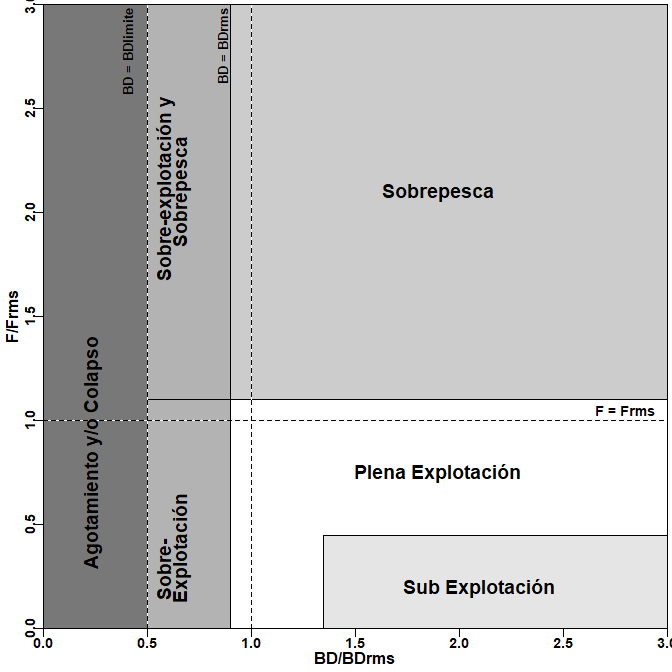
\includegraphics[width=0.6\textwidth]{FigurasInforme_Marzo/Figura13.png}
\end{center}

\small

\textbf{Figura 13}. Diagrama de fase definido por el CCT-PP para las
pesquerías de pelágicos pequeños. \vspace{0.5cm}

\normalsize

El estado de la pesquería en Plena Explotación se define en la Ley de
Pesca como ``un nivel en el que el punto biológico ha alcanzado o está a
su máximo rendimiento sostenido''. Debido a la variabilidad natural en
las condiciones ecológicas y ambientales, F\textsubscript{RMS} no es
estática, pero fluctuará alrededor de BD\textsubscript{RMS}. Para
reconocer esta variabilidad, una definición operativa para la región de
Plena Explotación se define que se extiende a ambos lados de los puntos
de referencia de RMS. Adicionalmente, el CCT-PP incorporó el concepto de
sobrepesca, precisó algunas definiciones y se pronunció respecto a la
zona de plena explotación, según consta en acta N°5 (11 al 14 de
noviembre de 2014). Los aspectos más relevantes son los que a
continuación se describen:

\begin{itemize}
\item
  \emph{Sobrepesca}: Este Comité consideró necesario diferenciar al
  interior de la zona de sobreexplotación definida por la LGPA, el área
  de sobrepesca, con el objeto de aplicar las medidas de Administración
  más acordes con dicha condición. En tal sentido, la sobrepesca
  ocurriría cuando la mortalidad por pesca F (variable de flujo y de
  control) exceda un valor considerado umbral o límite, que en este caso
  corresponde al valor superior en mortalidad por pesca (valor relativo
  al objetivo), de la zona de plena explotación.
\item
  \emph{Sobreexplotado}: En correspondencia con la definición anterior,
  la sobreexplotación ocurriría cuando la biomasa (variable de estado)
  cae bajo un valor umbral o límite, correspondiendo éste al valor
  inferior en biomasa (valor relativo al objetivo) de la zona de plena
  explotación.
\item
  \emph{Rango de Plena Explotación}: El CCT-PP recomendó por consenso
  los siguientes rangos que definen la condición de Plena Explotación de
  los recursos pelágicos, considerando los siguientes límites en biomasa
  y el correspondiente par ordenado en mortalidad por pesca:

  \begin{enumerate}
  \def\labelenumi{\alph{enumi})}
  \tightlist
  \item
    \emph{Límite bajo el objetivo de manejo} = 10\% Bajo
    BD\textsubscript{RMS}: Este criterio tiene como propósito el
    establecimiento de una banda estrecha en torno al RMS, que genere un
    área no deseada pequeña que en lo posible sea menor o igual al área
    de incertidumbre total del sistema, donde la biomasa está bajo la
    biomasa objetivo y a su vez, la mortalidad por pesca es mayor a la
    mortalidad por pesca objetivo. En consecuencia, el CCT-PP considera
    las numerosas recomendaciones en ciencia pesquera, respecto al
    riesgo de llevar a los stocks a una condición de sobreexplotación
    cuando se utiliza el RMS como objetivo de manejo, utiliza el
    concepto conforme al marco legal vigente y simultáneamente lo deja
    operando en la práctica, como un punto biológico de referencia
    límite.
  \item
    \emph{Límite sobre el objetivo de manejo} =75\% BD\textsubscript{0}
    (o 35\% sobre BD\textsubscript{RMS}): Para estos efectos el Comité
    rescató elementos del enfoque ecosistémico en especies de forraje,
    planteado recientemente por Pickitch \emph{et al}. (2012).
  \end{enumerate}
\end{itemize}

\hypertarget{objetivo-especuxedfico-3}{%
\subsection{3.3. Objetivo específico
3:}\label{objetivo-especuxedfico-3}}

\vspace{-0.2cm}

\emph{``Determinar niveles de Captura Biológicamente Aceptable (CBA) que
lleven y/o mantenga la pesquería en torno al Rendimiento Máximo
Sostenible (RMS), a partir de un análisis de riesgo en condiciones de
incertidumbre de no alcanzar los objetivos de conservación y
sostenibilidad conforme lo establece la LGPA y contenidos en el Plan de
Manejo y/o en el Programa de Recuperación respectivo, según
corresponda.''}

\hypertarget{captura-bioluxf3gicamente-aceptable-cba-1}{%
\subsubsection{3.3.1. Captura biológicamente aceptable
(CBA)}\label{captura-bioluxf3gicamente-aceptable-cba-1}}

\hypertarget{descripciuxf3n-del-proceso-de-cuxe1lculo-de-cba-para-cada-etapa-del-procedimiento-de-manejo}{%
\paragraph{Descripción del proceso de cálculo de CBA para cada etapa del
procedimiento de
manejo:}\label{descripciuxf3n-del-proceso-de-cuxe1lculo-de-cba-para-cada-etapa-del-procedimiento-de-manejo}}

La pesquería de sardina común ha sido manejada históricamente de manera
monoespecífica, considerando la incertidumbre asociada a la evaluación
de stock. El objetivo de conservación para ésta pesquería establece un
nivel de biomasa reproductiva o desovante equivalente al
55\%BD\textsubscript{0} del stock desovante en estado virginal (sin
explotación), con una estrategia de explotación que consiste en aplicar
una tasa de explotación constante, equivalente a la mortalidad por pesca
F que determina el 55\%BD0, definidas como F60\%BDPR establecido por el
Comité Científico Técnico Pesquerías de Pequeños Pelágicos (CCT-PP) para
resguardar la incertidumbre en el éxito de la clase anual que reclutaría
a la pesquería (Informe Técnico CCT-PP N°01/2015 \footnote{\url{http://www.subpesca.cl/portal/616/articles-87217_documento.pdf}}).

De acuerdo al ciclo de manejo histórico de esta pesquería
(\textbf{Figura 14}), la recomendación de CBA comienza después de la
veda reproductiva, donde se reporta la CBA inicial, y que permitirá al
CCT-PP establecer el estatus y recomendar el rango de CBA para el año
siguiente. En enero de cada año, el crucero de evaluación hidroacústico
permite estimar la abundancia y biomasa de reclutas (crucero de verano,
RECLAS), esta información junto a datos provenientes de la pesquería es
utilizada para la primera revisión de la CBA. En marzo se inicia el
período de extracción y en mayo se realiza el segundo crucero de
evaluación acústica (crucero de otoño, PELACES) para actualizar el
estatus y revisar una vez más la CBA.

La \textbf{Tabla 13} detalla la información disponible en cada etapa de
cálculo de CBA 2021, destacando que en la primera etapa de estimación
(CBA inicial) no se cuenta con información actualizada de los años
biológicos 2020-2021 y 2021-2022, por lo tanto, la población debe ser
proyectada dos años biológicos hacia el futuro (a inicios de julio de un
año a junio del año siguiente) para realizar el cálculo de la CBA 2021
en año calendario. En la segunda etapa (1era revisión) contamos con
información parcial del año biológico 2020-2021 y en la tercera etapa
(2da revisión) con información casi completa del año biológico
2020-2021. Sin embargo, para realizar el cálculo de la CBA 2021 en año
calendario, en ambas etapas es necesario proyectar un año biológico
hacia el futuro (2021-2022).

\begin{center}
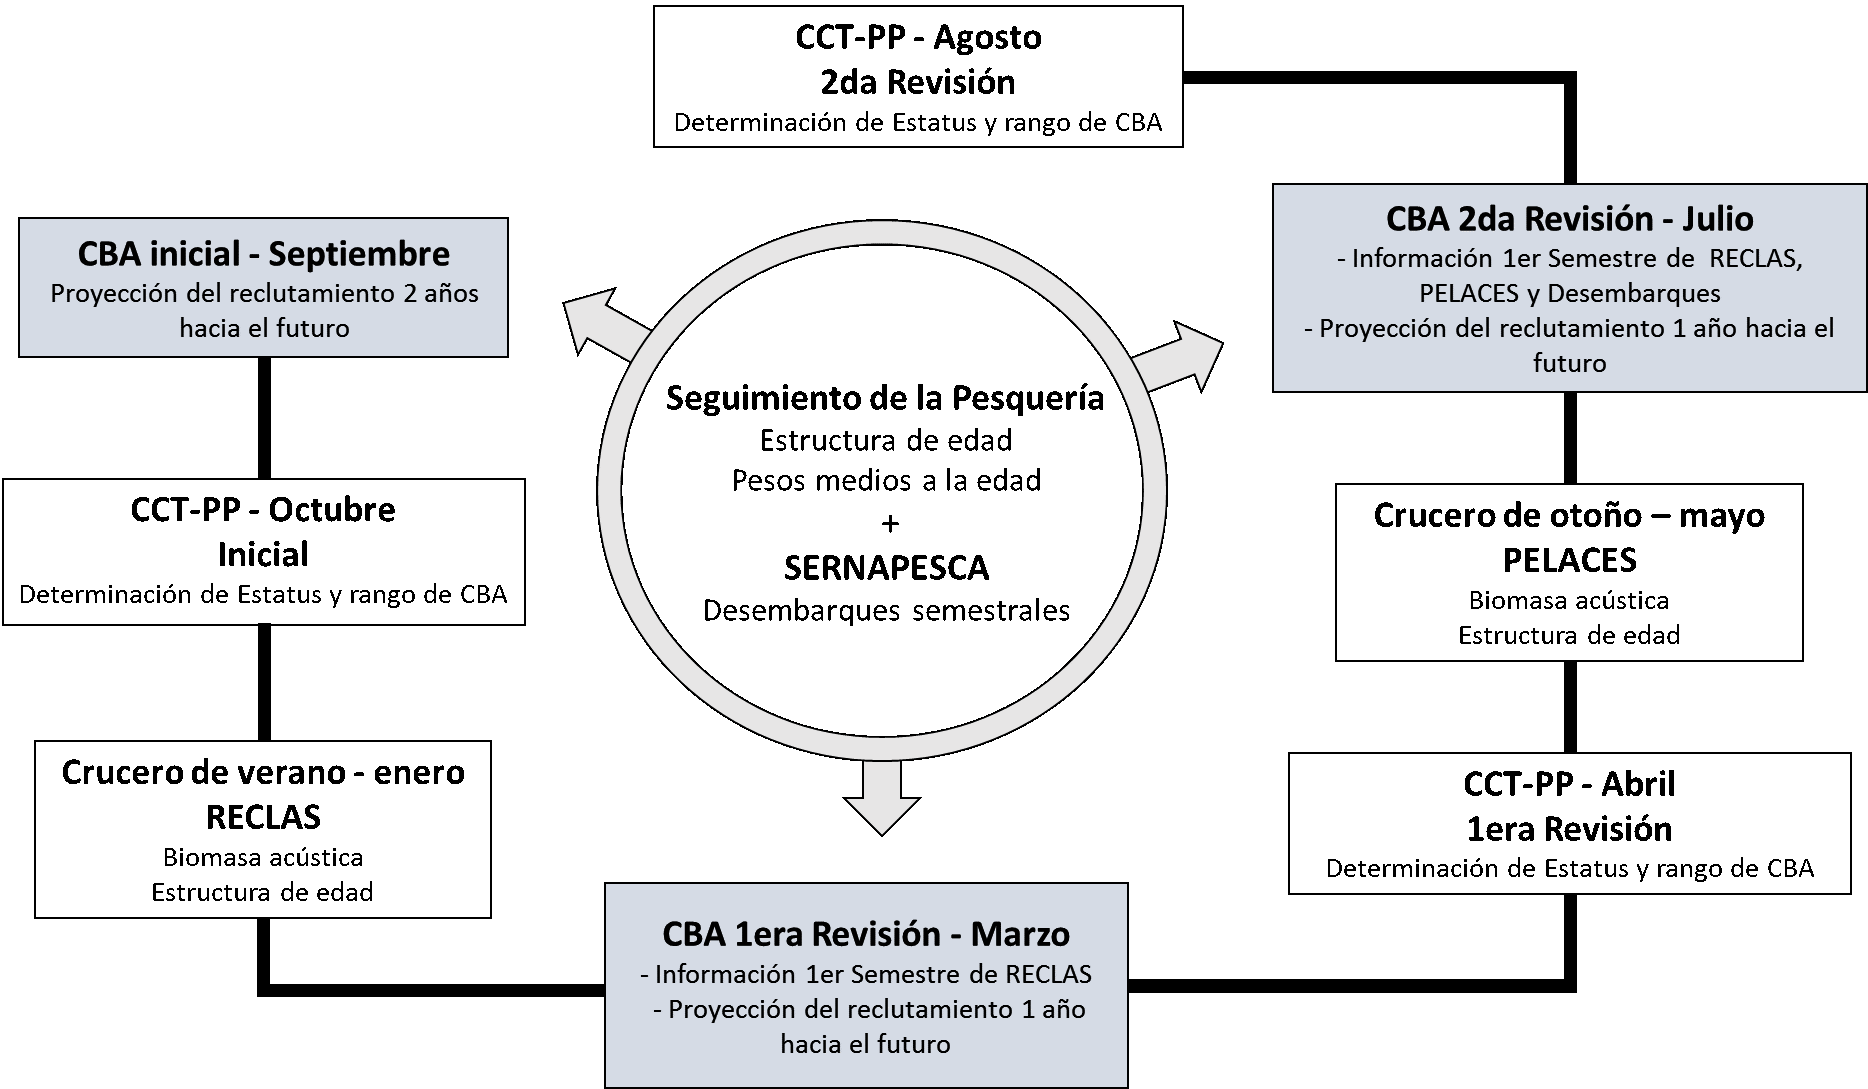
\includegraphics[width=0.9\textwidth]{FigurasInforme_Marzo/Figura14.png}
\end{center}

\small

\textbf{Figura 14}. Procedimiento de manejo actual para sardina común
centro-sur. \vspace{0.5cm} \normalsize

\small

\begin{center} 
 \textbf{Tabla 13.}
 \end{center}
 \begin{center} 
 \vspace{-0.2cm} Información relevante para el cálculo de CBA 2021 en cada una de las etapas de estimación.
 \end{center}
 \vspace{-0.2cm}

\begin{table}[h]
    \centering
    \resizebox{16cm}{!} {
    \begin{tabular}{|l|c|c|c|}
    \hline
  Datos de entrada  & CBA INICIAL                & 1ERA REVISIÓN                   & 2DA REVISIÓN  \\ 
  al modelo         & Septiembre 2020          & Marzo 2021                      & Julio 2021 \\ \hline
  Desembarques      &                            & Julio 1991- junio 2020 +        & Julio 1991 - \\
                    & Julio 1991 - junio 2020  & Supuesto de captura 2020/2021   & preliminar a junio 2021 \\
                    &                          &                                   &  \\ \hline
  Biomasa acústica  & 2000 – 2020                & 2000 – 2021                     &    2000 – 2021 \\
  Crucero de verano &                          &                                 & \\ \hline
  Biomasa acústica  & 2003 – 2020              & 2003 – 2020                     & 2003 – 2021 \\
  Crucero de otoño  &                          &                                 & \\ \hline
  Composición de    & Julio 1991 - junio 2020  & Julio 1991 - junio 2020         & Julio 1991 - mayo 2021  \\
  edad Flota        &                          &                                 & \\ \hline
  Composición de    & 2001 – 2020              & 2001 – 2021                       & 2001 – 2021 \\
  edad Cruceros de verano&                     &                                 & \\ \hline
  Composición de    & 2007 – 2020              & 2007 – 2020                     & 2007 – 2021 \\
  edad Cruceros de otoño&                      &                                 & \\ \hline
                    &                          & Julio 1990 - junio 2020         & \\
  Pesos medios      & Julio 1991 - junio 2020  & Promedio de los últimos 5 años  & Julio 1990 - mayo 2021 \\
  a la edad         &                          & de la serie histórica para      & \\ 
                    &                          & julio 2020-junio 2021           & \\ \hline
  Madurez sexual    & Constante                & Constante                       & Constante \\
  a la edad         &                          &                                 & \\ \hline
  Mortalidad natural& Constante                & Constante                       & Constante \\ \hline
  Proyección del    & 2 años biológicos        & 1 año biológico                 & 1 año biológico \\
  reclutamiento     & (años 2020/21 y 2021/22) & (año 2021/22)                   & (año 2021/22) \\ \hline
    \end{tabular}}
        \end{table}

\vspace{0.2cm}

\normalsize

El proceso de cálculo de la CBA 2021 para las tres etapas del ciclo de
manejo de sardina común (\textbf{Tabla 14}) consistirá en los siguientes
pasos:

\textbf{Paso 1}: Estimación de la captura proyectada
(Yp\textsubscript{RMS}) en año biológico aplicando los siguientes
supuestos:

\begin{itemize}
\tightlist
\item
  Escenarios de reclutamiento proyectado
\item
  Supuesto de pesos medios igual al promedio de los últimos 5 años de la
  serie
\item
  Mortalidad por pesca igual a F\textsubscript{RMS}
\end{itemize}

\textbf{Paso 2}: Estimación de la captura (Y\textsubscript{RMS}) del año
biológico actual aplicando los siguientes supuestos:

\begin{itemize}
\tightlist
\item
  Reclutamiento actualizado en asesoría de marzo o julio.
\item
  Pesos medios igual al promedio de los últimos 5 años (asesoría de
  marzo) o pesos medios actualizados (asesoría de julio).
\item
  Mortalidad por pesca equivalente al supuesto de captura igual a CBA
  inicial (asesoría de marzo) o mortalidad por pesca equivalente a la
  captura actualizada (asesoría de julio).
\end{itemize}

\textbf{Paso 3}: Estimación de la Captura Biológicamente Aceptable (CBA)
en año calendario aplicando los siguentes supuestos.

\begin{itemize}
\tightlist
\item
  Proporción de captura semestral (ps1, primer semestre y ps2, segundo
  semestre).
\item
  Probabilidad que la captura exceda el objetivo de manejo
  F\textsubscript{RMS}=F60\%BDPR.
\item
  Porcentaje de resguardo de la Captura al RMS.
\end{itemize}

\vspace{0.5cm}
\small

\begin{center} 
 \textbf{Tabla 14.}
 \end{center}
 \begin{center} 
 \vspace{-0.2cm} Métodos de estimación de la CBA 2021 para las tres etapas del ciclo de manejo de sardina común.
 \end{center}
 \vspace{-0.2cm}

\begin{table}[h]
  \centering
  \resizebox{12cm}{!} {
  \begin{tabular}{|l|c|c|}
  \hline
  Mes de Asesoría & Etapas de cálculo      & Métodos de estimación \\ \hline
  Septiembre 2020 & $CBA_{inicial}$      & $p_{s1} * Yp_{RMS(t+1)} + p_{s2} * Yp_{RMS(t+2)}$ \\
  Marzo 2021      & $CBA_{1eraRevisión}$ & $p_{s1} * Y_{RMS(t)} + p_{s2} * Yp_{RMS(t+1)}$ \\
  Julio 2021      & $CBA_{2daRevisión}$  & $p_{s1} * Y_{RMS(t)} + p_{s2} * Yp_{RMS(t+1)}$ \\ \hline
  \end{tabular}}
    \end{table}

\normalsize

\hypertarget{paso-1-captura-proyectada-yprms-en-auxf1o-bioluxf3gico-aplicando-frms}{%
\paragraph{\texorpdfstring{Paso 1: Captura proyectada
(Yp\textsubscript{RMS}) en año biológico aplicando
F\textsubscript{RMS}}{Paso 1: Captura proyectada (YpRMS) en año biológico aplicando FRMS}}\label{paso-1-captura-proyectada-yprms-en-auxf1o-bioluxf3gico-aplicando-frms}}

\hypertarget{escenarios-de-proyecciuxf3n-basada-en-distintos-niveles-de-reclutamiento}{%
\subparagraph{Escenarios de proyección basada en distintos niveles de
reclutamiento:}\label{escenarios-de-proyecciuxf3n-basada-en-distintos-niveles-de-reclutamiento}}

Se realiza un análisis de quiebres que consiste en un análisis
estadístico que permite detectar cambios en la serie histórica de los
reclutamientos estimados por el modelo de evaluación de stock. Para ello
se realizó un análisis de cambios estructurales en series de tiempo
(también conocido como detección de puntos de quiebre) implementado en
la librería ``strucchange'' del software R,
\url{https://cran.r-project.org/web/packages/strucchange/strucchange.pdf}.

\begin{Shaded}
\begin{Highlighting}[]
\KeywordTok{library}\NormalTok{(strucchange)}
\NormalTok{bp.nile \textless{}{-}}\StringTok{ }\KeywordTok{breakpoints}\NormalTok{(Reclutamientos }\OperatorTok{\textasciitilde{}}\StringTok{ }\DecValTok{1}\NormalTok{)}
\NormalTok{fm1 \textless{}{-}}\StringTok{ }\KeywordTok{lm}\NormalTok{(Reclutamientos }\OperatorTok{\textasciitilde{}}\StringTok{ }\KeywordTok{breakfactor}\NormalTok{(bp.nile, }\DataTypeTok{breaks =} \DecValTok{2}\NormalTok{))}
\NormalTok{puntos\_quiebres\textless{}{-}}\KeywordTok{fitted}\NormalTok{(fm1)}
\end{Highlighting}
\end{Shaded}

La \textbf{Figura 15} muestra tres niveles de reclutamiento detectados
por el análisis de quiebres de la serie histórica: a) un escenario
desfavorable que consiste en el reclutamiento promedio del período
1991-2007 (113 mil millones de ind.), b) un escenario favorable que
corresponde al promedio de los reclutamientos del período 2008 - 2012
(405 mil millones de ind.) y un escenario que representa el período
reciente entre el 2013-2021 (180 mil millones de ind.).

\begin{center}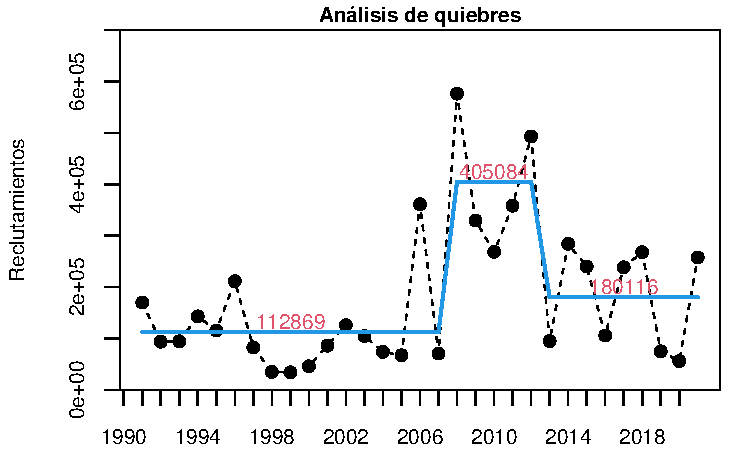
\includegraphics{FigurasInforme_Marzo/antecedentes_Reclproy_sept-1} \end{center}

\small

\textbf{Figura 15}. Análisis de quiebres de la serie histórica de los
reclutamientos de sardina común. \vspace{0.5cm} \normalsize

\hypertarget{supuesto-de-pesos-medios-a-la-edad-utilizado-en-la-proyecciuxf3n}{%
\subparagraph{Supuesto de pesos medios a la edad utilizado en la
proyección
:}\label{supuesto-de-pesos-medios-a-la-edad-utilizado-en-la-proyecciuxf3n}}

En relación a los pesos medios a la edad utilizados en la proyección del
stock y cálculo de CBA, se utiliza el promedio de los últimos 5 años
(\textbf{Figura 16}). Este supuesto fue acordado con el CCT-PP en la
sesión 02/2019 \footnote{\url{http://www.subpesca.cl/portal/616/articles-105403_documento.pdf}}.

\begin{center}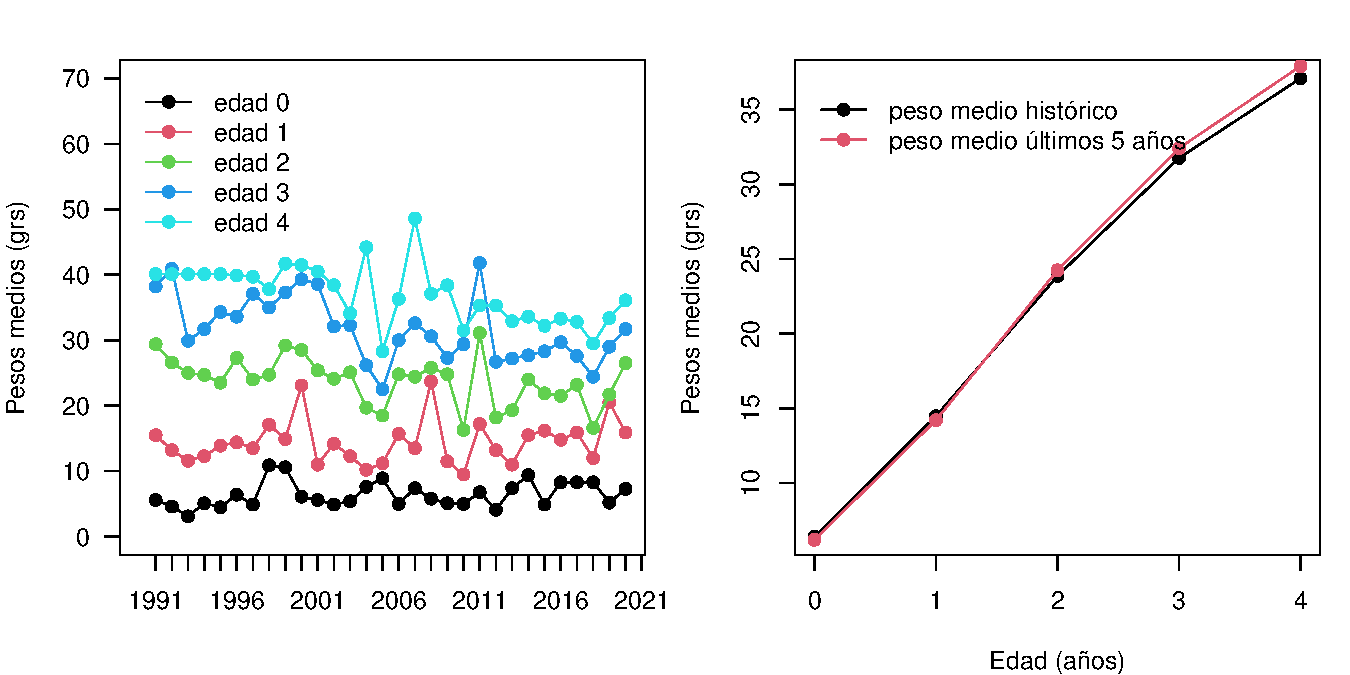
\includegraphics{FigurasInforme_Marzo/metod_datos_pesosmedios-1} \end{center}

\small

\textbf{Figura 16}. a) Variabilidad de los pesos medios de cada grupo de
edad (edad 0 a 4) y b) comparación del supuesto de pesos medios igual al
promedio histórico vs peso promedio de los últimos 5 años de la serie.
\vspace{0.5cm} \normalsize

\pagebreak

Los pasos siguientes son proyectar la población para la estimación de la
Captura en número y peso con una estrategia de explotación que consiste
en aplicar una tasa de explotación constante, equivalente a la
mortalidad por pesca F\textsubscript{RMS} en año biológico
(\textbf{Tabla 15}). \vspace{0.5cm}

\small
\begin{center} 
\textbf{Tabla 15.}
\end{center}
\begin{center} 
\vspace{-0.2cm} Proceso de estimación de la Captura ($Yp_{RMS}$) proyectada en año biológico aplicando $F_{RMS}$.
\end{center}
\vspace{-0.2cm}

\begin{longtable}[]{@{}ll@{}}
\toprule
\begin{minipage}[b]{0.57\columnwidth}\raggedright
Descripción\strut
\end{minipage} & \begin{minipage}[b]{0.37\columnwidth}\raggedright
Ecuación\strut
\end{minipage}\tabularnewline
\midrule
\endhead
\begin{minipage}[t]{0.57\columnwidth}\raggedright
Condición de partida para la proyección\strut
\end{minipage} & \begin{minipage}[t]{0.37\columnwidth}\raggedright
\(N_p=N_{naños}\), \(S_p=S_{naños}\)\strut
\end{minipage}\tabularnewline
\begin{minipage}[t]{0.57\columnwidth}\raggedright
Escenario de reclutamientos:R reclutamiento promedio de los años
iniciales entre los años 1991-2007, n es el número de años
iniciales\strut
\end{minipage} & \begin{minipage}[t]{0.37\columnwidth}\raggedright
\(Rp_{(a=0)}=\frac{\sum{R_{(1991-2007)}}}{n_{(1991-2007)}}\)\strut
\end{minipage}\tabularnewline
\begin{minipage}[t]{0.57\columnwidth}\raggedright
Escenario de reclutamiento:R reclutamiento promedio entre los años
2008-2012, n es el número de años del período\strut
\end{minipage} & \begin{minipage}[t]{0.37\columnwidth}\raggedright
\(Rp_{(a=0)}=\frac{\sum{R_{(2008-2012)}}}{n_{(2008-2012)}}\)\strut
\end{minipage}\tabularnewline
\begin{minipage}[t]{0.57\columnwidth}\raggedright
Escenario de reclutamientos:R reclutamiento promedio entre los años 2013
- año actual, n es el número de años del período\strut
\end{minipage} & \begin{minipage}[t]{0.37\columnwidth}\raggedright
\(Rp_{(a=0)}=\frac{\sum{R_{(2013-añoactual)}}}{n_{(2013-año actual)}}\)\strut
\end{minipage}\tabularnewline
\begin{minipage}[t]{0.57\columnwidth}\raggedright
Mortalidad por pesca y total al RMS\strut
\end{minipage} & \begin{minipage}[t]{0.37\columnwidth}\raggedright
\(F_{RMS}=sel_{naños} F60(%BDPR)
\), \(Z_{RMS}=F_{RMS}+M\), \(Sp=exp(-Z_{RMS} )\)\strut
\end{minipage}\tabularnewline
\begin{minipage}[t]{0.57\columnwidth}\raggedright
Dinámica de la abundancia proyectada\strut
\end{minipage} & \begin{minipage}[t]{0.37\columnwidth}\raggedright
\(Np_(a=0)=Rp\), \(Np_{(a+1)}=Np_{(a-1)} S_p\),
\(Np_{(a=4)}=Np_{(a-1)} S_p+Np_{(a=4)} S_p\)\strut
\end{minipage}\tabularnewline
\begin{minipage}[t]{0.57\columnwidth}\raggedright
Captura en número proyectada\strut
\end{minipage} & \begin{minipage}[t]{0.37\columnwidth}\raggedright
\(Cp_{RMS}=F_{RMS}/Z_{RMS}*Np(1-exp(-Z_{RMS})\))\strut
\end{minipage}\tabularnewline
\begin{minipage}[t]{0.57\columnwidth}\raggedright
Captura en peso proyectada\strut
\end{minipage} & \begin{minipage}[t]{0.37\columnwidth}\raggedright
\(Yp_{RMS}=\sum{Cp_{RMS}* w_{5años}^{med}}\)\strut
\end{minipage}\tabularnewline
\bottomrule
\end{longtable}

\normalsize

Donde, \(N_{naños}\) es la abundancia a la edad del último año de
evaluación, \(S_{naños}\) es la sobrevivencia del último año de
evaluación, \(R_p\) corresponde al reclutamiento proyectado al año
\(t\), sel\_naños es la selectividad edad específica del último año de
evaluación, \(F_{60}\) corresponde a la mortalidad por pesca que
determina el 55\%BD0 establecido por el (CCT-PP), \(Z_{RMS}\) es la
mortalidad total al RMS, \(M\) es la mortalidad natural, \(Np_{(a=0)}\)
es el reclutamiento proyectado, \(Np_{(a+1)}\) es la abundancia en
número a la edad \(a+1\), \(Cp_{RMS}\) es la captura proyectada en
número, \(Yp_{RMS}\) es la captura en peso proyectada y
\(w_{5años}^{med}\) corresponde al peso promedio de los últimos 5 años.

\hypertarget{paso-2-captura-del-auxf1o-actual-yrms-aplicando-frms}{%
\paragraph{\texorpdfstring{Paso 2: Captura del año actual
(Y\textsubscript{RMS}) aplicando
F\textsubscript{RMS}:}{Paso 2: Captura del año actual (YRMS) aplicando FRMS:}}\label{paso-2-captura-del-auxf1o-actual-yrms-aplicando-frms}}

Esta captura es estimada en la 1era y 2da revisión de CBA (asesorías de
marzo y julio), cuando se cuenta con información del año biológico
actualizado con las biomasas acústicas de los cruceros de verano y otoño
respectivamente y otras fuentes de información.

Captura en número del año biológico actual
\(C_{RMS}=\frac{F_{RMS}}{Z_{RMS}} N_{naños}(1-exp(-Z_{RMS}))\)

Captura en peso del año biológico actual
\(Y_{RMS}=\sum{C_{RMS} w_{5años}^{med}}\)

\hypertarget{paso-3-estimaciuxf3n-de-la-captura-bioluxf3gicamente-aceptable-cba}{%
\paragraph{Paso 3: Estimación de la Captura Biológicamente Aceptable
(CBA):}\label{paso-3-estimaciuxf3n-de-la-captura-bioluxf3gicamente-aceptable-cba}}

Considerando que el modelo de evaluación de stock de sardina común
emplea información agregada en año biológico, la población es proyectada
uno o dos años biológicos hacia el futuro (a inicios de julio de un año
a junio del año siguiente). Por consiguiente, el cálculo de la captura
en año calendario se obtiene como el promedio ponderado según la
estacionalidad semestral de la pesquería. El análisis de quiebres de la
serie de proporción de desembarques del primer semestre muestra que a
partir del 2010 la proporción disminuye en torno al 70\% para el primer
semestre (\textbf{Figura 17}). De este modo, el cálculo de CBA se
obtiene como el promedio ponderado según la estacionalidad semestral de
la pesquería del período más reciente en 70\% para el primer semestre y
30\% para el segundo semestre del año calendario. Este supuesto fue
acordado con el CCT-PP en la sesión 02/2019 \footnote{\url{http://www.subpesca.cl/portal/616/articles-105403_documento.pdf}}.

\begin{center}
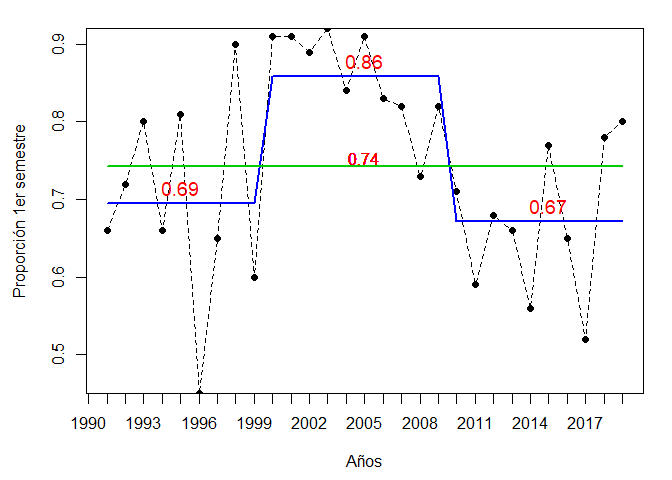
\includegraphics[width=1\textwidth]{FigurasInforme_Marzo/Fig17_metod_cbaprop.png}
\end{center}

\small

\textbf{Figura 17}. Serie histórica de la proporción de los desembarques
durante el primer semestre.

\vspace{0.5cm} \normalsize

\hypertarget{percentiles-de-probabilidad-de-sobrepasar-el-objetivo-de-manejo-frms}{%
\subparagraph{\texorpdfstring{Percentiles de probabilidad de sobrepasar
el objetivo de manejo
F\textsubscript{RMS}:}{Percentiles de probabilidad de sobrepasar el objetivo de manejo FRMS:}}\label{percentiles-de-probabilidad-de-sobrepasar-el-objetivo-de-manejo-frms}}

Se considera el establecimiento de un percentil entre un 10\% - 50\% de
probabilidad de sobrepasar el objetivo de manejo igual a
F\textsubscript{RMS}. El percentil corresponde a una distribución de
probabilidad acumulada y representa la probabilidad de estar en
sobrepesca (\textbf{Figura 18}). El CCT-PP determina el rango de CBA
seleccionado el percentil de probabilidad y escenario de reclutamiento
proyectado. Dado la alta incertidumbre existente en el momento de
definir la CBA inicial, el CCT-PP selecciona el escenario de
reclutamiento más precautorio y un percentil de probabilidad inferior al
50\%. Este percentil de probabilidad es equivalente a un nivel de
resguardo que se calcula a partir de la captura estimada para cada
percentil de probabilidad y la captura al RMS, de este modo, se tiene un
nivel de referencia de cuanto se está resguardando considerando el hito
de revisión de CBA o condición del recurso.

\vspace{0.5cm}
\large
\begin{center} 
$Resguardo = 1-\frac{Captura(i)}{Captura_{RMS}}, i = percentil.de.captura (10\% ...50\%)$
\end{center}
\vspace{0.5cm}

\normalsize

Donde la Captura(i) es la captura estimada para cada percentil de
probabilidad (10\% - 50\%) y Captura\textsubscript{RMS} corresponde a la
media (50\% probabilidad).

\begin{center}
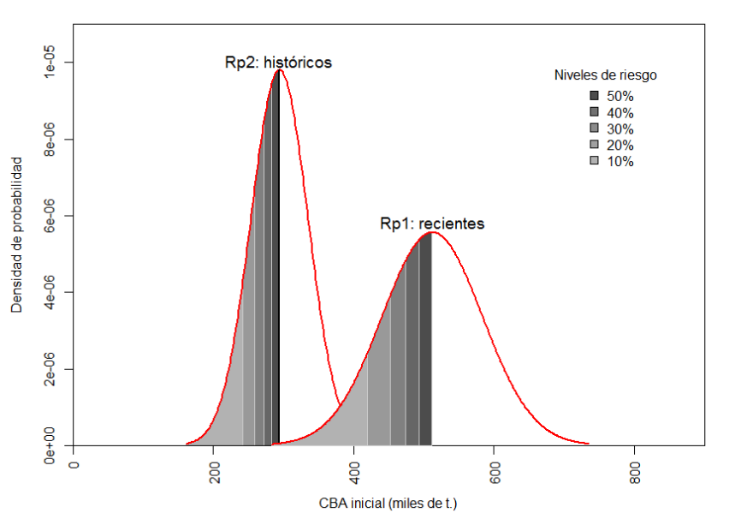
\includegraphics[width=1\textwidth]{FigurasInforme_Marzo/Fig18_metod_cbapercentil.png}
\end{center}

\small

\textbf{Figura 18}. CBA inicial ante percentiles de captura y bajo dos
escenarios de reclutamiento. \vspace{0.5cm} \normalsize

\hypertarget{paso-4-incorporaciuxf3n-del-descarte-en-la-cba}{%
\paragraph{Paso 4: Incorporación del descarte en la
CBA:}\label{paso-4-incorporaciuxf3n-del-descarte-en-la-cba}}

La actual Ley General de Pesca y Acuicultura (LGPA, N° 18.892) persigue
la conservación y el uso sustentable de los recursos pesqueros mediante
la aplicación del enfoque precautorio y ecosistémico, garantizando el
resguardo de los ecosistemas marinos. En este contexto, el Artículo 7°B
de la LGPA indica que no podrá realizarse el descarte de individuos de
una especie objetivo, cualquiera sea su régimen de acceso, y su fauna
acompañante, salvo que se i) haya fijado una cuota global anual de
captura para la especie objetivo y, ii) que en el proceso de
establecimiento de la cuota global anual de captura se haya considerado
el descarte, entre otras restricciones indicadas por el citado artículo.

Para dar cumplimiento a esta normativa se estima una \(CBA_{total}\) que
da cuenta de toda la mortalidad por pesca incluido el descarte. El
CCT-PP debe establecer el rango de CBA que se construye a partir de una
CBA máxima (\(CBA_{max}\)), es decir, el rango por ley es
(\(0,8*CBA_{max}; CBA_{max}\)). Esta \(CBA_{max}\), deberá estimarse a
partir de la \(CBA_{total}\) descontando el porcentaje de descarte
supuesto para el año 2021. La proporción del descarte (pd) supuesto para
el año 2021 y que deberá ser descontado de la \(CBA_{total}\) para
establecer la \(CBA_{max}\).

\vspace{0.5cm}
\large
\begin{center} 
$CBA_{max}=CBA_{total}-pd*CBA_{total}$
\end{center}
\vspace{0.5cm}

\normalsize

\hypertarget{proyecciuxf3n-del-stock}{%
\subsubsection{3.3.2. Proyección del
stock}\label{proyecciuxf3n-del-stock}}

Se analiza las probables trayectorias de la biomasa desovante como
consecuencia de la aplicación de mortalidad por pesca igual a
F\textsubscript{RMS} y dos ponderadores de F\textsubscript{RMS} igual a
0,9 y 0,7, considerando la incertidumbre del estatus (e.g., matriz de
varianza/covarianza de ADMB) y los posibles estados de la naturaleza a
futuro (e.g., niveles probables de reclutamiento futuro, escenarios de
reclutamiento). Lo anterior permite analizar los niveles de riesgo de no
alcanzar el objetivo de manejo BD\textsubscript{RMS} en el mediano plazo
(2 años biológicos hacia el futuro), considerando la incertidumbre del
estatus (probabilidad de sobre-explotación y/o colapso) y los probables
estados de la naturaleza a futuro.

\pagebreak

\hypertarget{objetivo-especuxedfico-4}{%
\subsection{3.4. Objetivo específico
4:}\label{objetivo-especuxedfico-4}}

\vspace{-0.2cm}

\emph{``Informar el avance del Programa de Mejoramiento Continuo de la
Calidad en la Asesoría Científica (PMCCAC) realizado durante el presente
estudio, respecto al cumplimiento de recomendaciones formuladas en
procesos de RPEI y priorizadas por el CCT, cuando corresponda.''}

Se informan los avances alcanzados durante el desarrollo de este
estudio, conforme al Programa de Mejoramiento Continuo de la Calidad de
la Asesoría Científica (PMCCAC), elaborado por recurso y/o pesquería.
Este PMCCAC no sólo se enfoca en las brechas de datos, información y
conocimiento, sino que incluye la pertinencia, consistencia, calidad y
coherencia de éstos con la situación general de la pesquería, acorde con
los requerimientos de asesoría solicitados por la administración
pesquera. Con esto, se desarrolla un análisis de la incertidumbre
involucrada en los datos e información utilizada en la evaluación.

En este sentido, todo lo referido a sistemas o procesos fuera del
alcance de este estudio (i.e., información disponible, nivel de
conocimiento del recurso, etc.) son consignados para conocimiento y
fines de administración pesquera. No obstante, en el ámbito de
responsabilidad directa de este estudio, se informa de todas las
recomendaciones realizadas en el Taller de Revisión Por Pares Externa e
Independiente (RPPEI) con el objetivo de lograr la mejor aplicación del
EME, conforme al estándar de análisis de la pesquería. Sobre la base de
lo anterior, se incorporan los ajustes necesarios, proponiendo las
acciones, actividades, metas, plazos y condiciones que se consideren
necesarios para lograr disminuir las brechas identificadas y los
requerimientos para alcanzar los estándares de asesoría previamente
definidos.

A continuación, se detalla el contenido presentado la \textbf{Sección
4.4} de este informe:

\begin{itemize}
\item
  Esquema de trabajo y plan de actividades 2017-2018 acordado con
  SUBPESCA.
\item
  Mejoras realizadas al modelo de evaluación de stock
\item
  Avance en la reducción de brechas.

  \begin{itemize}
  \tightlist
  \item
    Actividades desarrolladas durante el año 2018
  \item
    Actividades desarrolladas durante el año 2019
  \item
    Actividades desarrolladas durante el año 2020
  \end{itemize}
\item
  Recomendaciones realizadas en Revisión por Pares Externa e
  independiente (RPEI).
\item
  Recomendaciones realizadas en Informe de evaluación técnica de
  proyectos del programa de investigación básica o permanente para la
  regulación pesquera y de acuicultura.
\end{itemize}

\pagebreak

\hypertarget{resultados}{%
\section{4. RESULTADOS}\label{resultados}}

\hypertarget{objetivo-especuxedfico-1-1}{%
\subsection{4.1. Objetivo específico
1:}\label{objetivo-especuxedfico-1-1}}

\vspace{-0.2cm}

\emph{``Implementar procedimientos de evaluación de stock basados en
protocolos científicos para la determinación del estatus de sardina
común, con arreglo al nivel de información, conocimiento e incertidumbre
correspondiente, conforme a los estándares actuales en ciencia
pesquera.''}

\hypertarget{datos-de-entrada-al-modelo-de-evaluaciuxf3n-de-stock-1}{%
\subsubsection{4.1.1. Datos de entrada al modelo de evaluación de
stock}\label{datos-de-entrada-al-modelo-de-evaluaciuxf3n-de-stock-1}}

El período de análisis de la evaluación de stock comienza en 1990/91
hasta el año 2020/21. A continuación, se detalla los datos actualizados
en la asesoría de marzo 2021 (\textbf{Figura 19}). \vspace{-0.2cm}

\hypertarget{datos-actualizados}{%
\paragraph{Datos actualizados}\label{datos-actualizados}}

\begin{itemize}
\tightlist
\item
  Biomasa del crucero acústico de enero 2021
\item
  Composición de edad del crucero acústico de enero 2021
\end{itemize}

\hypertarget{datos-supuestos}{%
\paragraph{Datos supuestos}\label{datos-supuestos}}

\quad

A la fecha aún no se cuenta con información pesquera del primer semestre
2021 que permita completar el año biológico 2010/21. Para estos casos se
utilizan los siguientes supuestos.

\begin{itemize}
\tightlist
\item
  \emph{Captura 2020/21 sin incorporar descarte}: Se asume igual a
  210.827 t. calculado desde el desembarque segundo semestre 2020
  (69.841 mil t.) más 0,7xCBA inicial 2021 (CBA 2021 = 201.409 t,
  70\%CBA2021 = 140.986 t.) (\textbf{Tabla 17})
\item
  \emph{Porcentaje de Descarte 2020/21}: Se asume igual a un 4\% de
  descarte (acordado en sesión del 25 de febrero del CCT-PP) lo que
  equivale a una captura descartada de 8.433 t. (\textbf{Tabla 17})
\item
  \emph{Captura 2020/21 con descarte incorporado}: 210.827 t. + 8.433 =
  219.260 t. (\textbf{Tabla 17})
\item
  \emph{Composición de edad de la flota 2020/21}: no ingresa valor
  (igual a 0)
\item
  \emph{Pesos medios e iniciales 2020/21}: Se asume pesos medios igual
  al promedio de los últimos 5 años. Los pesos iniciales son calculados
  en función de los pesos medios para el 2020/21 (detalles del cálculo
  en sección metodología).
\item
  \emph{Biomasa del crucero acústico de mayo 2021} no ingresa valor
  (igual a 0)
\item
  \emph{Composición de edad del crucero acústico de mayo 2021} no
  ingresa valor (igual a 0)
\end{itemize}

\vspace{-0.2cm}

\hypertarget{supuestos-de-proyecciuxf3n-de-1-auxf1o-bioluxf3gico-20212022}{%
\paragraph{Supuestos de proyección de 1 año biológico
2021/2022}\label{supuestos-de-proyecciuxf3n-de-1-auxf1o-bioluxf3gico-20212022}}

\begin{itemize}
\tightlist
\item
  Escenarios de reclutamiento promedio
\item
  Mortalidad por pesca igual a F\textsubscript{RMS}
\item
  Pesos igual al promedio últimos 5 años
\item
  Proporción de captura semestral 70/30
\end{itemize}

\vspace{-0.2cm}

\begin{center}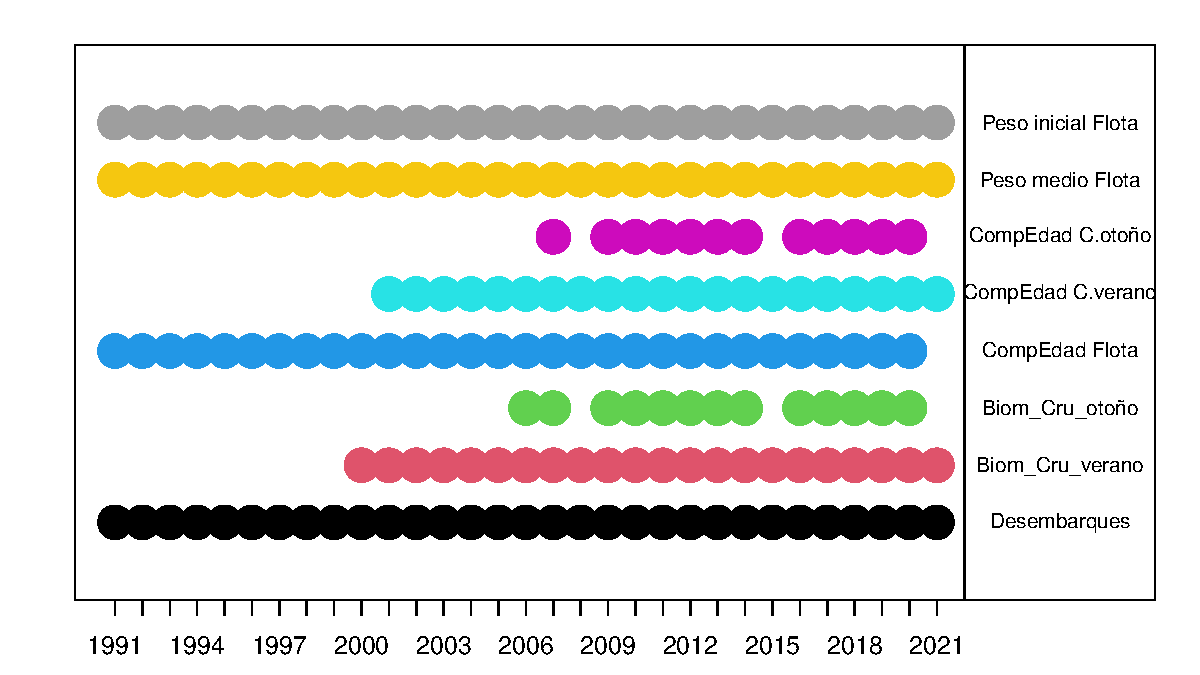
\includegraphics{FigurasInforme_Marzo/F19_datos-1} \end{center}

\vspace{-0.5cm}
\small

\textbf{Figura 19}. Series de tiempo de los datos de entrada al modelo
de evaluación de stock de sardina común de las Regiones de Valparaíso a
Los Lagos. \vspace{0.5cm} \normalsize

\hypertarget{descripciuxf3n-de-datos-de-entrada}{%
\paragraph{Descripción de datos de
entrada}\label{descripciuxf3n-de-datos-de-entrada}}

\quad

Una de las principales características del stock de sardina común es el
comportamiento estacional de las capturas, donde cerca del 70\% de la
captura total anual se obtiene al primer semestre de cada año, con
máximos entre marzo y abril. Esta estacionalidad es altamente
influenciada por el pulso de reclutamiento de enero, observándose una
fuerte relación entre la biomasa estimada por el crucero de enero y los
desembarques. Al respecto, se observa que durante los años 2015 al 2019,
las biomasas acústicas de verano se mantuvieron en niveles en torno a
los dos millones de toneladas, lo cual se ve reflejado también en una
estabilidad en las capturas en torno a las 330 mil toneladas. Por otro
lado, las biomasas acústicas estimadas por el crucero de otoño reflejan
el efecto de la remoción ejercidas por la pesca y causas naturales, con
biomasas en general menores a las estimadas en el crucero de verano, en
torno a 1,5 millones de toneladas (\textbf{Tabla 16} y \textbf{Figura
20}).

No obstante, para el año 2020 la biomasa estimada por el crucero
acústico de verano se redujo a un millón de toneladas (54\% menor al
2019), la biomasa del crucero de otoño disminuye un 40\% respecto al
2019 y las capturas 2019/20 se redujeron un 9\% respecto al año previo.
El desembarque 2020 está en torno a las 258.092 toneladas, equivalente a
un 80\% de la CBA 2020 recomentada por el CCT\_PP (321.307 toneladas).

La biomasa total estimada por el crucero de enero 2021 retorno a los
niveles observados entre el 2013 al 2019 (2,36 millones de t.),
incrementando un 125\% respecto a lo estimado para el año 2020
(\textbf{Tabla 16} y \textbf{Figura 20}). En relación a la captura
2020/21 se asume una reducción del 24\% respecto del año biológico
2019/20, no obstante la captura 2020/21 es un supuesto que debe ser
actualizado en la asesoría de julio 2021 con datos de desembarque del
primer semestre 2021 (\textbf{Tabla 17}).

\pagebreak

\small
\begin{center} 
\textbf{Tabla 16.}
\end{center}
\begin{center} 
\vspace{-0.2cm} Índices de abundancia utilizadas en la evaluación de stock de sardina común provenientes de los cruceros de Verano (RECLAS), Otoño (PELACES), crucero de huevos (MPDH).
\end{center}
\vspace{-0.2cm}

\begin{longtable}[]{@{}cccc@{}}
\toprule
\begin{minipage}[b]{0.16\columnwidth}\centering
Año

calendario\strut
\end{minipage} & \begin{minipage}[b]{0.22\columnwidth}\centering
Biomasa crucero

de verano

(toneladas)\strut
\end{minipage} & \begin{minipage}[b]{0.22\columnwidth}\centering
Biomasa crucero

de otoño

(toneladas)\strut
\end{minipage} & \begin{minipage}[b]{0.25\columnwidth}\centering
Biomasa desovante

MPDH

(toneladas)\strut
\end{minipage}\tabularnewline
\midrule
\endhead
\begin{minipage}[t]{0.16\columnwidth}\centering
1991\strut
\end{minipage} & \begin{minipage}[t]{0.22\columnwidth}\centering
\strut
\end{minipage} & \begin{minipage}[t]{0.22\columnwidth}\centering
\strut
\end{minipage} & \begin{minipage}[t]{0.25\columnwidth}\centering
\strut
\end{minipage}\tabularnewline
\begin{minipage}[t]{0.16\columnwidth}\centering
1992\strut
\end{minipage} & \begin{minipage}[t]{0.22\columnwidth}\centering
\strut
\end{minipage} & \begin{minipage}[t]{0.22\columnwidth}\centering
\strut
\end{minipage} & \begin{minipage}[t]{0.25\columnwidth}\centering
\strut
\end{minipage}\tabularnewline
\begin{minipage}[t]{0.16\columnwidth}\centering
1993\strut
\end{minipage} & \begin{minipage}[t]{0.22\columnwidth}\centering
\strut
\end{minipage} & \begin{minipage}[t]{0.22\columnwidth}\centering
\strut
\end{minipage} & \begin{minipage}[t]{0.25\columnwidth}\centering
\strut
\end{minipage}\tabularnewline
\begin{minipage}[t]{0.16\columnwidth}\centering
1994\strut
\end{minipage} & \begin{minipage}[t]{0.22\columnwidth}\centering
\strut
\end{minipage} & \begin{minipage}[t]{0.22\columnwidth}\centering
\strut
\end{minipage} & \begin{minipage}[t]{0.25\columnwidth}\centering
\strut
\end{minipage}\tabularnewline
\begin{minipage}[t]{0.16\columnwidth}\centering
1995\strut
\end{minipage} & \begin{minipage}[t]{0.22\columnwidth}\centering
\strut
\end{minipage} & \begin{minipage}[t]{0.22\columnwidth}\centering
\strut
\end{minipage} & \begin{minipage}[t]{0.25\columnwidth}\centering
\strut
\end{minipage}\tabularnewline
\begin{minipage}[t]{0.16\columnwidth}\centering
1996\strut
\end{minipage} & \begin{minipage}[t]{0.22\columnwidth}\centering
\strut
\end{minipage} & \begin{minipage}[t]{0.22\columnwidth}\centering
\strut
\end{minipage} & \begin{minipage}[t]{0.25\columnwidth}\centering
\strut
\end{minipage}\tabularnewline
\begin{minipage}[t]{0.16\columnwidth}\centering
1997\strut
\end{minipage} & \begin{minipage}[t]{0.22\columnwidth}\centering
\strut
\end{minipage} & \begin{minipage}[t]{0.22\columnwidth}\centering
\strut
\end{minipage} & \begin{minipage}[t]{0.25\columnwidth}\centering
\strut
\end{minipage}\tabularnewline
\begin{minipage}[t]{0.16\columnwidth}\centering
1998\strut
\end{minipage} & \begin{minipage}[t]{0.22\columnwidth}\centering
\strut
\end{minipage} & \begin{minipage}[t]{0.22\columnwidth}\centering
\strut
\end{minipage} & \begin{minipage}[t]{0.25\columnwidth}\centering
\strut
\end{minipage}\tabularnewline
\begin{minipage}[t]{0.16\columnwidth}\centering
1999\strut
\end{minipage} & \begin{minipage}[t]{0.22\columnwidth}\centering
\strut
\end{minipage} & \begin{minipage}[t]{0.22\columnwidth}\centering
\strut
\end{minipage} & \begin{minipage}[t]{0.25\columnwidth}\centering
\strut
\end{minipage}\tabularnewline
\begin{minipage}[t]{0.16\columnwidth}\centering
2000\strut
\end{minipage} & \begin{minipage}[t]{0.22\columnwidth}\centering
252.601\strut
\end{minipage} & \begin{minipage}[t]{0.22\columnwidth}\centering
\strut
\end{minipage} & \begin{minipage}[t]{0.25\columnwidth}\centering
\strut
\end{minipage}\tabularnewline
\begin{minipage}[t]{0.16\columnwidth}\centering
2001\strut
\end{minipage} & \begin{minipage}[t]{0.22\columnwidth}\centering
567.819\strut
\end{minipage} & \begin{minipage}[t]{0.22\columnwidth}\centering
\strut
\end{minipage} & \begin{minipage}[t]{0.25\columnwidth}\centering
\strut
\end{minipage}\tabularnewline
\begin{minipage}[t]{0.16\columnwidth}\centering
2002\strut
\end{minipage} & \begin{minipage}[t]{0.22\columnwidth}\centering
844.713\strut
\end{minipage} & \begin{minipage}[t]{0.22\columnwidth}\centering
\strut
\end{minipage} & \begin{minipage}[t]{0.25\columnwidth}\centering
498.337\strut
\end{minipage}\tabularnewline
\begin{minipage}[t]{0.16\columnwidth}\centering
2003\strut
\end{minipage} & \begin{minipage}[t]{0.22\columnwidth}\centering
477.998\strut
\end{minipage} & \begin{minipage}[t]{0.22\columnwidth}\centering
\strut
\end{minipage} & \begin{minipage}[t]{0.25\columnwidth}\centering
\strut
\end{minipage}\tabularnewline
\begin{minipage}[t]{0.16\columnwidth}\centering
2004\strut
\end{minipage} & \begin{minipage}[t]{0.22\columnwidth}\centering
351.125\strut
\end{minipage} & \begin{minipage}[t]{0.22\columnwidth}\centering
\strut
\end{minipage} & \begin{minipage}[t]{0.25\columnwidth}\centering
5.186\strut
\end{minipage}\tabularnewline
\begin{minipage}[t]{0.16\columnwidth}\centering
2005\strut
\end{minipage} & \begin{minipage}[t]{0.22\columnwidth}\centering
339.783\strut
\end{minipage} & \begin{minipage}[t]{0.22\columnwidth}\centering
\strut
\end{minipage} & \begin{minipage}[t]{0.25\columnwidth}\centering
125.008\strut
\end{minipage}\tabularnewline
\begin{minipage}[t]{0.16\columnwidth}\centering
2006\strut
\end{minipage} & \begin{minipage}[t]{0.22\columnwidth}\centering
2.178.397\strut
\end{minipage} & \begin{minipage}[t]{0.22\columnwidth}\centering
552.880\strut
\end{minipage} & \begin{minipage}[t]{0.25\columnwidth}\centering
\strut
\end{minipage}\tabularnewline
\begin{minipage}[t]{0.16\columnwidth}\centering
2007\strut
\end{minipage} & \begin{minipage}[t]{0.22\columnwidth}\centering
2.134.043\strut
\end{minipage} & \begin{minipage}[t]{0.22\columnwidth}\centering
188.675\strut
\end{minipage} & \begin{minipage}[t]{0.25\columnwidth}\centering
168.611\strut
\end{minipage}\tabularnewline
\begin{minipage}[t]{0.16\columnwidth}\centering
2008\strut
\end{minipage} & \begin{minipage}[t]{0.22\columnwidth}\centering
4.813.144\strut
\end{minipage} & \begin{minipage}[t]{0.22\columnwidth}\centering
\strut
\end{minipage} & \begin{minipage}[t]{0.25\columnwidth}\centering
109.162\strut
\end{minipage}\tabularnewline
\begin{minipage}[t]{0.16\columnwidth}\centering
2009\strut
\end{minipage} & \begin{minipage}[t]{0.22\columnwidth}\centering
1.555.625\strut
\end{minipage} & \begin{minipage}[t]{0.22\columnwidth}\centering
991.730\strut
\end{minipage} & \begin{minipage}[t]{0.25\columnwidth}\centering
213.762\strut
\end{minipage}\tabularnewline
\begin{minipage}[t]{0.16\columnwidth}\centering
2010\strut
\end{minipage} & \begin{minipage}[t]{0.22\columnwidth}\centering
2.623.565\strut
\end{minipage} & \begin{minipage}[t]{0.22\columnwidth}\centering
2.467.720\strut
\end{minipage} & \begin{minipage}[t]{0.25\columnwidth}\centering
579.715\strut
\end{minipage}\tabularnewline
\begin{minipage}[t]{0.16\columnwidth}\centering
2011\strut
\end{minipage} & \begin{minipage}[t]{0.22\columnwidth}\centering
3.216.857\strut
\end{minipage} & \begin{minipage}[t]{0.22\columnwidth}\centering
1.416.034\strut
\end{minipage} & \begin{minipage}[t]{0.25\columnwidth}\centering
649.985\strut
\end{minipage}\tabularnewline
\begin{minipage}[t]{0.16\columnwidth}\centering
2012\strut
\end{minipage} & \begin{minipage}[t]{0.22\columnwidth}\centering
3.843.000\strut
\end{minipage} & \begin{minipage}[t]{0.22\columnwidth}\centering
1.217.169\strut
\end{minipage} & \begin{minipage}[t]{0.25\columnwidth}\centering
157.893\strut
\end{minipage}\tabularnewline
\begin{minipage}[t]{0.16\columnwidth}\centering
2013\strut
\end{minipage} & \begin{minipage}[t]{0.22\columnwidth}\centering
1.133.477\strut
\end{minipage} & \begin{minipage}[t]{0.22\columnwidth}\centering
2.296.489\strut
\end{minipage} & \begin{minipage}[t]{0.25\columnwidth}\centering
87.575\strut
\end{minipage}\tabularnewline
\begin{minipage}[t]{0.16\columnwidth}\centering
2014\strut
\end{minipage} & \begin{minipage}[t]{0.22\columnwidth}\centering
3.079.434\strut
\end{minipage} & \begin{minipage}[t]{0.22\columnwidth}\centering
1.805.815\strut
\end{minipage} & \begin{minipage}[t]{0.25\columnwidth}\centering
83.554\strut
\end{minipage}\tabularnewline
\begin{minipage}[t]{0.16\columnwidth}\centering
2015\strut
\end{minipage} & \begin{minipage}[t]{0.22\columnwidth}\centering
1.972.148\strut
\end{minipage} & \begin{minipage}[t]{0.22\columnwidth}\centering
\strut
\end{minipage} & \begin{minipage}[t]{0.25\columnwidth}\centering
\strut
\end{minipage}\tabularnewline
\begin{minipage}[t]{0.16\columnwidth}\centering
2016\strut
\end{minipage} & \begin{minipage}[t]{0.22\columnwidth}\centering
2.032.684\strut
\end{minipage} & \begin{minipage}[t]{0.22\columnwidth}\centering
1.482.799\strut
\end{minipage} & \begin{minipage}[t]{0.25\columnwidth}\centering
\strut
\end{minipage}\tabularnewline
\begin{minipage}[t]{0.16\columnwidth}\centering
2017\strut
\end{minipage} & \begin{minipage}[t]{0.22\columnwidth}\centering
2.025.002\strut
\end{minipage} & \begin{minipage}[t]{0.22\columnwidth}\centering
1.565.315\strut
\end{minipage} & \begin{minipage}[t]{0.25\columnwidth}\centering
\strut
\end{minipage}\tabularnewline
\begin{minipage}[t]{0.16\columnwidth}\centering
2018\strut
\end{minipage} & \begin{minipage}[t]{0.22\columnwidth}\centering
2.424.330\strut
\end{minipage} & \begin{minipage}[t]{0.22\columnwidth}\centering
1.577.507\strut
\end{minipage} & \begin{minipage}[t]{0.25\columnwidth}\centering
\strut
\end{minipage}\tabularnewline
\begin{minipage}[t]{0.16\columnwidth}\centering
2019\strut
\end{minipage} & \begin{minipage}[t]{0.22\columnwidth}\centering
2.275.425\strut
\end{minipage} & \begin{minipage}[t]{0.22\columnwidth}\centering
1.421.176\strut
\end{minipage} & \begin{minipage}[t]{0.25\columnwidth}\centering
\strut
\end{minipage}\tabularnewline
\begin{minipage}[t]{0.16\columnwidth}\centering
2020\strut
\end{minipage} & \begin{minipage}[t]{0.22\columnwidth}\centering
1.050.175\strut
\end{minipage} & \begin{minipage}[t]{0.22\columnwidth}\centering
867.257\strut
\end{minipage} & \begin{minipage}[t]{0.25\columnwidth}\centering
\strut
\end{minipage}\tabularnewline
\begin{minipage}[t]{0.16\columnwidth}\centering
2021\strut
\end{minipage} & \begin{minipage}[t]{0.22\columnwidth}\centering
2.363.380\strut
\end{minipage} & \begin{minipage}[t]{0.22\columnwidth}\centering
\strut
\end{minipage} & \begin{minipage}[t]{0.25\columnwidth}\centering
\strut
\end{minipage}\tabularnewline
\bottomrule
\end{longtable}

\pagebreak

\small
\begin{center} 
\textbf{Tabla 17.}
\end{center}
\begin{center} 
\vspace{-0.2cm}  Desembarques en toneladas, porcentaje de descarte supuesto, captura descartada (toneladas) y captura total (toneladas) estimadas en año biológico para sardina común de las Regiones de Valparaíso a Los Lagos.
\end{center}
\vspace{-0.2cm}

\begin{longtable}[]{@{}ccccc@{}}
\toprule
\begin{minipage}[b]{0.14\columnwidth}\centering
Año.biológico\strut
\end{minipage} & \begin{minipage}[b]{0.16\columnwidth}\centering
Desembarques.t.\strut
\end{minipage} & \begin{minipage}[b]{0.19\columnwidth}\centering
Porcentaje.descarte\strut
\end{minipage} & \begin{minipage}[b]{0.21\columnwidth}\centering
Captura.descartada.t.\strut
\end{minipage} & \begin{minipage}[b]{0.16\columnwidth}\centering
Captura.total.t.\strut
\end{minipage}\tabularnewline
\midrule
\endhead
\begin{minipage}[t]{0.14\columnwidth}\centering
1990-91\strut
\end{minipage} & \begin{minipage}[t]{0.16\columnwidth}\centering
494567\strut
\end{minipage} & \begin{minipage}[t]{0.19\columnwidth}\centering
0\%\strut
\end{minipage} & \begin{minipage}[t]{0.21\columnwidth}\centering
0\strut
\end{minipage} & \begin{minipage}[t]{0.16\columnwidth}\centering
494567\strut
\end{minipage}\tabularnewline
\begin{minipage}[t]{0.14\columnwidth}\centering
1991-92\strut
\end{minipage} & \begin{minipage}[t]{0.16\columnwidth}\centering
514787\strut
\end{minipage} & \begin{minipage}[t]{0.19\columnwidth}\centering
0\%\strut
\end{minipage} & \begin{minipage}[t]{0.21\columnwidth}\centering
0\strut
\end{minipage} & \begin{minipage}[t]{0.16\columnwidth}\centering
514787\strut
\end{minipage}\tabularnewline
\begin{minipage}[t]{0.14\columnwidth}\centering
1992-93\strut
\end{minipage} & \begin{minipage}[t]{0.16\columnwidth}\centering
250237\strut
\end{minipage} & \begin{minipage}[t]{0.19\columnwidth}\centering
0\%\strut
\end{minipage} & \begin{minipage}[t]{0.21\columnwidth}\centering
0\strut
\end{minipage} & \begin{minipage}[t]{0.16\columnwidth}\centering
250237\strut
\end{minipage}\tabularnewline
\begin{minipage}[t]{0.14\columnwidth}\centering
1993-94\strut
\end{minipage} & \begin{minipage}[t]{0.16\columnwidth}\centering
358949\strut
\end{minipage} & \begin{minipage}[t]{0.19\columnwidth}\centering
0\%\strut
\end{minipage} & \begin{minipage}[t]{0.21\columnwidth}\centering
0\strut
\end{minipage} & \begin{minipage}[t]{0.16\columnwidth}\centering
358949\strut
\end{minipage}\tabularnewline
\begin{minipage}[t]{0.14\columnwidth}\centering
1994-95\strut
\end{minipage} & \begin{minipage}[t]{0.16\columnwidth}\centering
361735\strut
\end{minipage} & \begin{minipage}[t]{0.19\columnwidth}\centering
0\%\strut
\end{minipage} & \begin{minipage}[t]{0.21\columnwidth}\centering
0\strut
\end{minipage} & \begin{minipage}[t]{0.16\columnwidth}\centering
361735\strut
\end{minipage}\tabularnewline
\begin{minipage}[t]{0.14\columnwidth}\centering
1995-96\strut
\end{minipage} & \begin{minipage}[t]{0.16\columnwidth}\centering
120608\strut
\end{minipage} & \begin{minipage}[t]{0.19\columnwidth}\centering
0\%\strut
\end{minipage} & \begin{minipage}[t]{0.21\columnwidth}\centering
0\strut
\end{minipage} & \begin{minipage}[t]{0.16\columnwidth}\centering
120608\strut
\end{minipage}\tabularnewline
\begin{minipage}[t]{0.14\columnwidth}\centering
1996-97\strut
\end{minipage} & \begin{minipage}[t]{0.16\columnwidth}\centering
552515\strut
\end{minipage} & \begin{minipage}[t]{0.19\columnwidth}\centering
0\%\strut
\end{minipage} & \begin{minipage}[t]{0.21\columnwidth}\centering
0\strut
\end{minipage} & \begin{minipage}[t]{0.16\columnwidth}\centering
552515\strut
\end{minipage}\tabularnewline
\begin{minipage}[t]{0.14\columnwidth}\centering
1997-98\strut
\end{minipage} & \begin{minipage}[t]{0.16\columnwidth}\centering
73892\strut
\end{minipage} & \begin{minipage}[t]{0.19\columnwidth}\centering
0\%\strut
\end{minipage} & \begin{minipage}[t]{0.21\columnwidth}\centering
0\strut
\end{minipage} & \begin{minipage}[t]{0.16\columnwidth}\centering
73892\strut
\end{minipage}\tabularnewline
\begin{minipage}[t]{0.14\columnwidth}\centering
1998-99\strut
\end{minipage} & \begin{minipage}[t]{0.16\columnwidth}\centering
212993\strut
\end{minipage} & \begin{minipage}[t]{0.19\columnwidth}\centering
0\%\strut
\end{minipage} & \begin{minipage}[t]{0.21\columnwidth}\centering
0\strut
\end{minipage} & \begin{minipage}[t]{0.16\columnwidth}\centering
212993\strut
\end{minipage}\tabularnewline
\begin{minipage}[t]{0.14\columnwidth}\centering
1999-00\strut
\end{minipage} & \begin{minipage}[t]{0.16\columnwidth}\centering
205616\strut
\end{minipage} & \begin{minipage}[t]{0.19\columnwidth}\centering
0\%\strut
\end{minipage} & \begin{minipage}[t]{0.21\columnwidth}\centering
0\strut
\end{minipage} & \begin{minipage}[t]{0.16\columnwidth}\centering
205616\strut
\end{minipage}\tabularnewline
\begin{minipage}[t]{0.14\columnwidth}\centering
2000-01\strut
\end{minipage} & \begin{minipage}[t]{0.16\columnwidth}\centering
50451\strut
\end{minipage} & \begin{minipage}[t]{0.19\columnwidth}\centering
4\%\strut
\end{minipage} & \begin{minipage}[t]{0.21\columnwidth}\centering
2018\strut
\end{minipage} & \begin{minipage}[t]{0.16\columnwidth}\centering
52469\strut
\end{minipage}\tabularnewline
\begin{minipage}[t]{0.14\columnwidth}\centering
2001-02\strut
\end{minipage} & \begin{minipage}[t]{0.16\columnwidth}\centering
305257\strut
\end{minipage} & \begin{minipage}[t]{0.19\columnwidth}\centering
4\%\strut
\end{minipage} & \begin{minipage}[t]{0.21\columnwidth}\centering
12210\strut
\end{minipage} & \begin{minipage}[t]{0.16\columnwidth}\centering
317467\strut
\end{minipage}\tabularnewline
\begin{minipage}[t]{0.14\columnwidth}\centering
2002-03\strut
\end{minipage} & \begin{minipage}[t]{0.16\columnwidth}\centering
282360\strut
\end{minipage} & \begin{minipage}[t]{0.19\columnwidth}\centering
4\%\strut
\end{minipage} & \begin{minipage}[t]{0.21\columnwidth}\centering
11294\strut
\end{minipage} & \begin{minipage}[t]{0.16\columnwidth}\centering
293654\strut
\end{minipage}\tabularnewline
\begin{minipage}[t]{0.14\columnwidth}\centering
2003-04\strut
\end{minipage} & \begin{minipage}[t]{0.16\columnwidth}\centering
372689\strut
\end{minipage} & \begin{minipage}[t]{0.19\columnwidth}\centering
4\%\strut
\end{minipage} & \begin{minipage}[t]{0.21\columnwidth}\centering
14908\strut
\end{minipage} & \begin{minipage}[t]{0.16\columnwidth}\centering
387597\strut
\end{minipage}\tabularnewline
\begin{minipage}[t]{0.14\columnwidth}\centering
2004-05\strut
\end{minipage} & \begin{minipage}[t]{0.16\columnwidth}\centering
242976\strut
\end{minipage} & \begin{minipage}[t]{0.19\columnwidth}\centering
4\%\strut
\end{minipage} & \begin{minipage}[t]{0.21\columnwidth}\centering
9719\strut
\end{minipage} & \begin{minipage}[t]{0.16\columnwidth}\centering
252695\strut
\end{minipage}\tabularnewline
\begin{minipage}[t]{0.14\columnwidth}\centering
2005-06\strut
\end{minipage} & \begin{minipage}[t]{0.16\columnwidth}\centering
496438\strut
\end{minipage} & \begin{minipage}[t]{0.19\columnwidth}\centering
4\%\strut
\end{minipage} & \begin{minipage}[t]{0.21\columnwidth}\centering
19858\strut
\end{minipage} & \begin{minipage}[t]{0.16\columnwidth}\centering
516296\strut
\end{minipage}\tabularnewline
\begin{minipage}[t]{0.14\columnwidth}\centering
2006-07\strut
\end{minipage} & \begin{minipage}[t]{0.16\columnwidth}\centering
344596\strut
\end{minipage} & \begin{minipage}[t]{0.19\columnwidth}\centering
4\%\strut
\end{minipage} & \begin{minipage}[t]{0.21\columnwidth}\centering
13784\strut
\end{minipage} & \begin{minipage}[t]{0.16\columnwidth}\centering
358380\strut
\end{minipage}\tabularnewline
\begin{minipage}[t]{0.14\columnwidth}\centering
2007-08\strut
\end{minipage} & \begin{minipage}[t]{0.16\columnwidth}\centering
713623\strut
\end{minipage} & \begin{minipage}[t]{0.19\columnwidth}\centering
4\%\strut
\end{minipage} & \begin{minipage}[t]{0.21\columnwidth}\centering
28545\strut
\end{minipage} & \begin{minipage}[t]{0.16\columnwidth}\centering
742168\strut
\end{minipage}\tabularnewline
\begin{minipage}[t]{0.14\columnwidth}\centering
2008-09\strut
\end{minipage} & \begin{minipage}[t]{0.16\columnwidth}\centering
905818\strut
\end{minipage} & \begin{minipage}[t]{0.19\columnwidth}\centering
4\%\strut
\end{minipage} & \begin{minipage}[t]{0.21\columnwidth}\centering
36233\strut
\end{minipage} & \begin{minipage}[t]{0.16\columnwidth}\centering
942051\strut
\end{minipage}\tabularnewline
\begin{minipage}[t]{0.14\columnwidth}\centering
2009-10\strut
\end{minipage} & \begin{minipage}[t]{0.16\columnwidth}\centering
603450\strut
\end{minipage} & \begin{minipage}[t]{0.19\columnwidth}\centering
4\%\strut
\end{minipage} & \begin{minipage}[t]{0.21\columnwidth}\centering
24138\strut
\end{minipage} & \begin{minipage}[t]{0.16\columnwidth}\centering
627588\strut
\end{minipage}\tabularnewline
\begin{minipage}[t]{0.14\columnwidth}\centering
2010-11\strut
\end{minipage} & \begin{minipage}[t]{0.16\columnwidth}\centering
796319\strut
\end{minipage} & \begin{minipage}[t]{0.19\columnwidth}\centering
4\%\strut
\end{minipage} & \begin{minipage}[t]{0.21\columnwidth}\centering
31853\strut
\end{minipage} & \begin{minipage}[t]{0.16\columnwidth}\centering
828172\strut
\end{minipage}\tabularnewline
\begin{minipage}[t]{0.14\columnwidth}\centering
2011-12\strut
\end{minipage} & \begin{minipage}[t]{0.16\columnwidth}\centering
826505\strut
\end{minipage} & \begin{minipage}[t]{0.19\columnwidth}\centering
4\%\strut
\end{minipage} & \begin{minipage}[t]{0.21\columnwidth}\centering
33060\strut
\end{minipage} & \begin{minipage}[t]{0.16\columnwidth}\centering
859565\strut
\end{minipage}\tabularnewline
\begin{minipage}[t]{0.14\columnwidth}\centering
2012,13\strut
\end{minipage} & \begin{minipage}[t]{0.16\columnwidth}\centering
402507\strut
\end{minipage} & \begin{minipage}[t]{0.19\columnwidth}\centering
4\%\strut
\end{minipage} & \begin{minipage}[t]{0.21\columnwidth}\centering
16100\strut
\end{minipage} & \begin{minipage}[t]{0.16\columnwidth}\centering
418607\strut
\end{minipage}\tabularnewline
\begin{minipage}[t]{0.14\columnwidth}\centering
2013-14\strut
\end{minipage} & \begin{minipage}[t]{0.16\columnwidth}\centering
500641\strut
\end{minipage} & \begin{minipage}[t]{0.19\columnwidth}\centering
4\%\strut
\end{minipage} & \begin{minipage}[t]{0.21\columnwidth}\centering
20026\strut
\end{minipage} & \begin{minipage}[t]{0.16\columnwidth}\centering
520667\strut
\end{minipage}\tabularnewline
\begin{minipage}[t]{0.14\columnwidth}\centering
2014-15\strut
\end{minipage} & \begin{minipage}[t]{0.16\columnwidth}\centering
401201\strut
\end{minipage} & \begin{minipage}[t]{0.19\columnwidth}\centering
4\%\strut
\end{minipage} & \begin{minipage}[t]{0.21\columnwidth}\centering
16048\strut
\end{minipage} & \begin{minipage}[t]{0.16\columnwidth}\centering
417249\strut
\end{minipage}\tabularnewline
\begin{minipage}[t]{0.14\columnwidth}\centering
2015-16\strut
\end{minipage} & \begin{minipage}[t]{0.16\columnwidth}\centering
289013\strut
\end{minipage} & \begin{minipage}[t]{0.19\columnwidth}\centering
4\%\strut
\end{minipage} & \begin{minipage}[t]{0.21\columnwidth}\centering
11561\strut
\end{minipage} & \begin{minipage}[t]{0.16\columnwidth}\centering
300574\strut
\end{minipage}\tabularnewline
\begin{minipage}[t]{0.14\columnwidth}\centering
2016-17\strut
\end{minipage} & \begin{minipage}[t]{0.16\columnwidth}\centering
399415\strut
\end{minipage} & \begin{minipage}[t]{0.19\columnwidth}\centering
2\%\strut
\end{minipage} & \begin{minipage}[t]{0.21\columnwidth}\centering
7988\strut
\end{minipage} & \begin{minipage}[t]{0.16\columnwidth}\centering
407403\strut
\end{minipage}\tabularnewline
\begin{minipage}[t]{0.14\columnwidth}\centering
2017-18\strut
\end{minipage} & \begin{minipage}[t]{0.16\columnwidth}\centering
348574\strut
\end{minipage} & \begin{minipage}[t]{0.19\columnwidth}\centering
2\%\strut
\end{minipage} & \begin{minipage}[t]{0.21\columnwidth}\centering
6971\strut
\end{minipage} & \begin{minipage}[t]{0.16\columnwidth}\centering
355545\strut
\end{minipage}\tabularnewline
\begin{minipage}[t]{0.14\columnwidth}\centering
2018-19\strut
\end{minipage} & \begin{minipage}[t]{0.16\columnwidth}\centering
301557\strut
\end{minipage} & \begin{minipage}[t]{0.19\columnwidth}\centering
6\%\strut
\end{minipage} & \begin{minipage}[t]{0.21\columnwidth}\centering
18093\strut
\end{minipage} & \begin{minipage}[t]{0.16\columnwidth}\centering
319650\strut
\end{minipage}\tabularnewline
\begin{minipage}[t]{0.14\columnwidth}\centering
2019-20\strut
\end{minipage} & \begin{minipage}[t]{0.16\columnwidth}\centering
273376\strut
\end{minipage} & \begin{minipage}[t]{0.19\columnwidth}\centering
6\%\strut
\end{minipage} & \begin{minipage}[t]{0.21\columnwidth}\centering
16403\strut
\end{minipage} & \begin{minipage}[t]{0.16\columnwidth}\centering
289779\strut
\end{minipage}\tabularnewline
\begin{minipage}[t]{0.14\columnwidth}\centering
2020-21\strut
\end{minipage} & \begin{minipage}[t]{0.16\columnwidth}\centering
210827\strut
\end{minipage} & \begin{minipage}[t]{0.19\columnwidth}\centering
4\%\strut
\end{minipage} & \begin{minipage}[t]{0.21\columnwidth}\centering
8433\strut
\end{minipage} & \begin{minipage}[t]{0.16\columnwidth}\centering
219260\strut
\end{minipage}\tabularnewline
\bottomrule
\end{longtable}

\begin{center}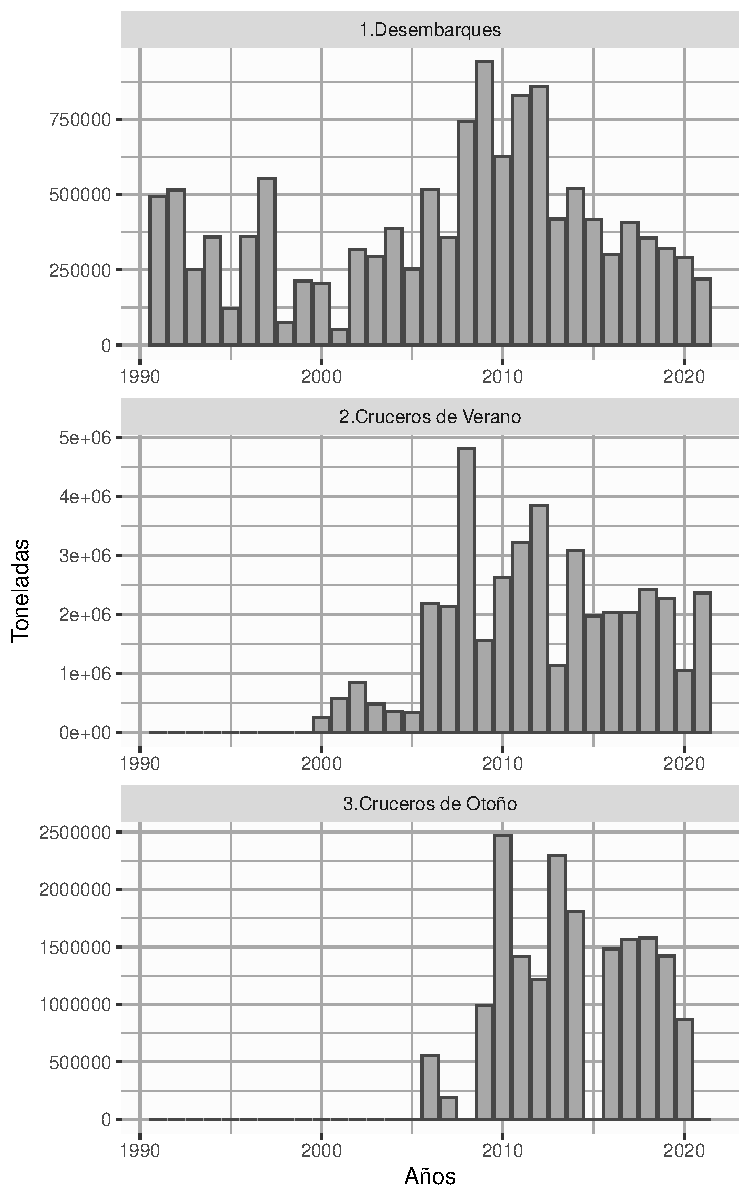
\includegraphics{FigurasInforme_Marzo/F20_datInd-1} \end{center}

\vspace{-0.5cm}
\small

\textbf{Figura 20}. Serie de desembarques y biomasas estimadas por la
evaluación hidroacústica de verano y otoño utilizadas como datos de
entrada al modelo de evaluación de stock de sardina común de las
Regiones de Valparaíso a Los Lagos. \vspace{0.5cm} \normalsize

\pagebreak

\hypertarget{composiciuxf3n-de-edad-y-pesos-medios}{%
\subparagraph{Composición de edad y pesos
medios}\label{composiciuxf3n-de-edad-y-pesos-medios}}

\quad

La pesquería de sardina común está sustentada principalmente por la
abundancia del grupo de edad 0, con una proporción en torno al 60-70\%
de la captura en número de la flota entre San Antonio-Corral. La captura
en número a la edad se caracteriza por presentar una alta variabilidad
interanual, siendo los años 2007, 2013, 2016, 2019 y 2020 los años con
menor proporción de reclutas. Los pesos medios del grupo de edad 0 se
encuentra en torno a los 8 grs. Se observa una estabilización de los
pesos medios a partir del 2013 para todos los grupos de edad
(\textbf{Figura 21} y \textbf{Figura 22}). En relación de la composición
de edad de los cruceros de verano se observa que el grupo de edad 0
representa el 80\% de la captura en número. Por otro lado, en el caso
del crucero de otoño, el grupo de edad 0 representa el 60\% de la
captura en número (\textbf{Figura 23} y \textbf{Figura 24}).

Los resultados del crucero de verano 2019 y 2020 presentan una
disminución en los niveles de abundancia de la fracción recluta, el
estimado de biomasa total del crucero de verano 2019 es sostenido por la
fracción adulta (edad 1+). Mientras que el estimado 2020 es sostenido
por individuos de edad 2+.

Esta disminución se confirma al actualizar la composición de edad de la
flota 2018/19 y 2019/20 y del crucero de otoño 2019 y 2020. Por lo
tanto, la disminución de la biomasa total 2020 estaría fuertemente
relacionada a la reducción del número de individuos de los grupos de
edad 0 y 1 principalmente.

Los resultados del crucero de verano 2021 muestran un incremento
significativo en los niveles de abundancia de la fracción recluta (94\%
individuos de edad 0), a diferencia de los dos años previos, la biomasa
total del crucero de verano 2021 es sostenido principalmente por la
fracción recluta (edad 0), observandose una baja presencia de individuos
adultos (edad 1+).

\begin{center}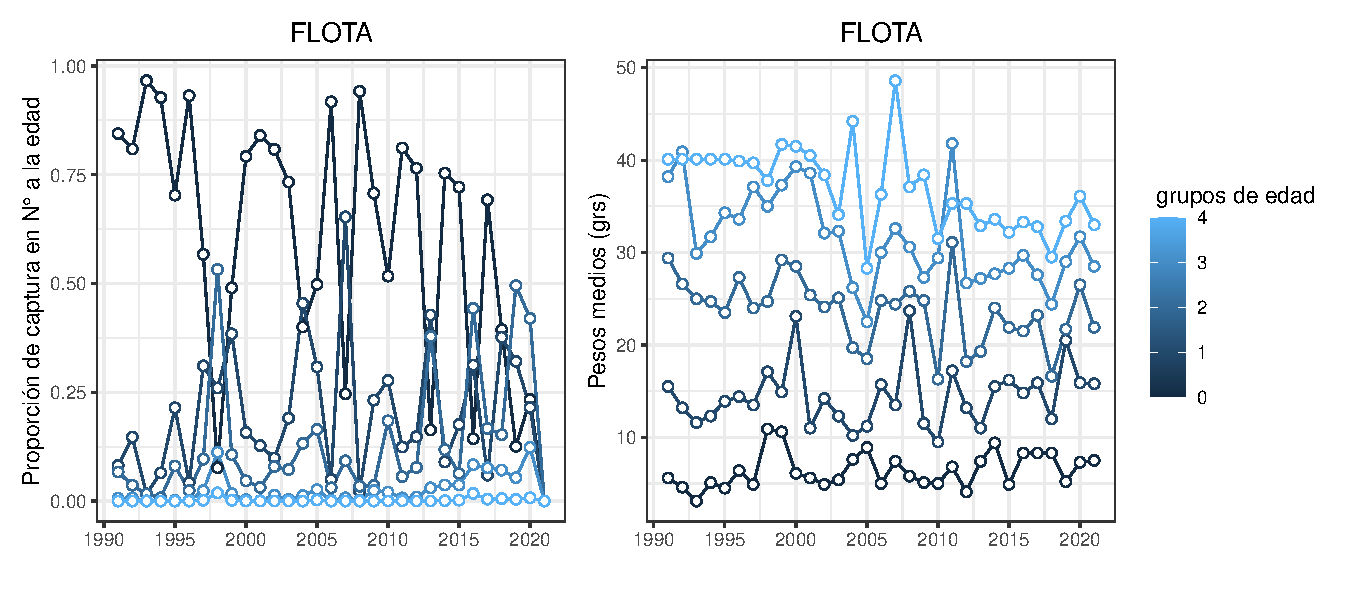
\includegraphics{FigurasInforme_Marzo/F21_datComp-1} \end{center}

\vspace{-0.5cm}
\small

\textbf{Figura 21}. Variabilidad interanual de la proporción de la
captura de la flota (panel izquierdo) y pesos medios (panel derecho) de
cada grupo de edad (edad 0 a 4) de sardina común de las Regiones de
Valparaíso a Los Lagos. \normalsize

\begin{center}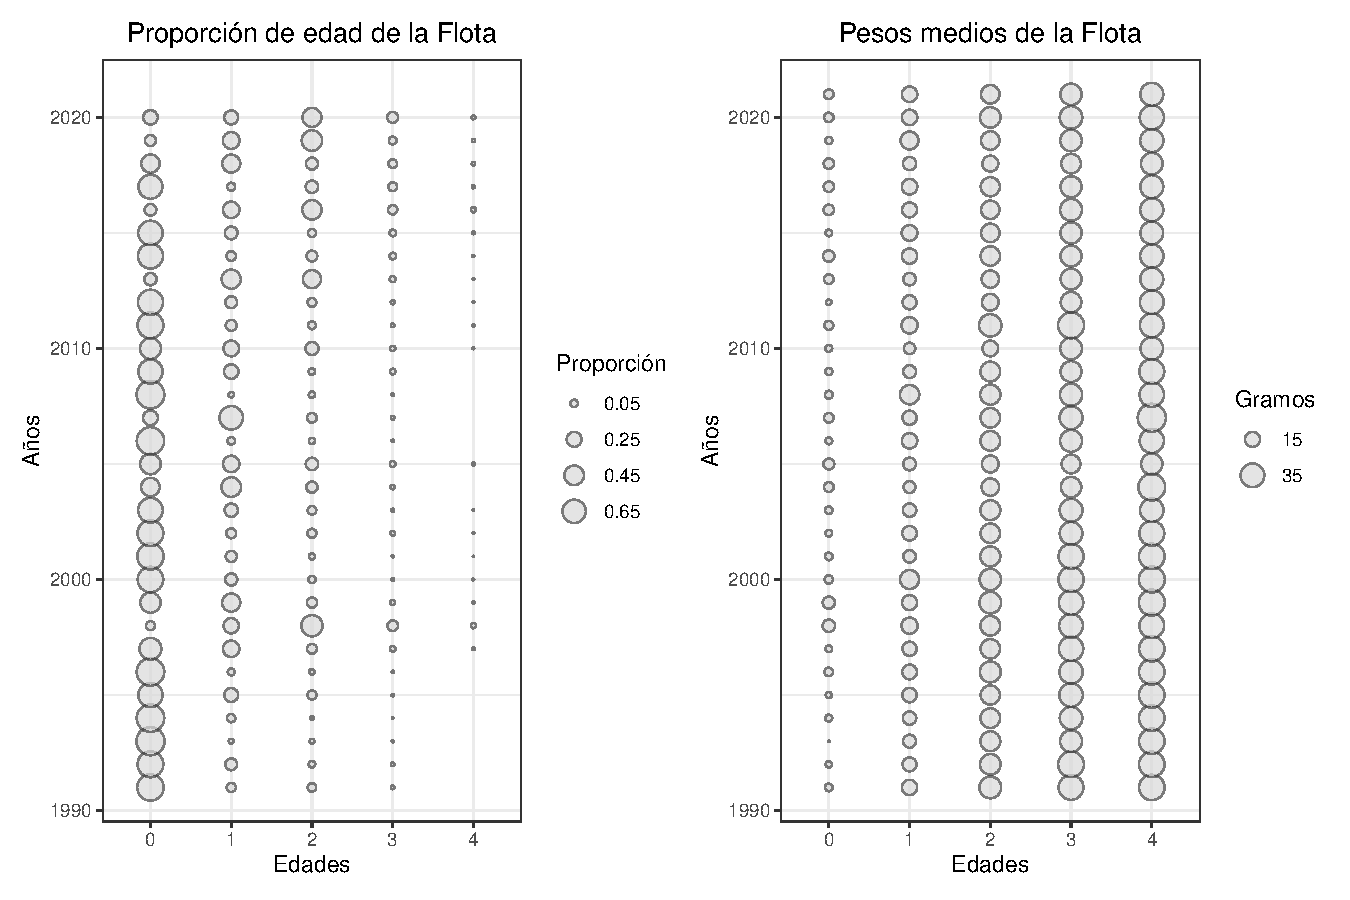
\includegraphics{FigurasInforme_Marzo/Fig22_datComp-1} \end{center}

\vspace{-0.5cm}
\small

\textbf{Figura 22}. Composición de edad de la captura de la flota (panel
izquierdo) y pesos medios (panel derecho) utilizados en la evaluación de
stock de sardina común de las Regiones de Valparaíso a Los Lagos.
\vspace{0.5cm} \normalsize

\begin{center}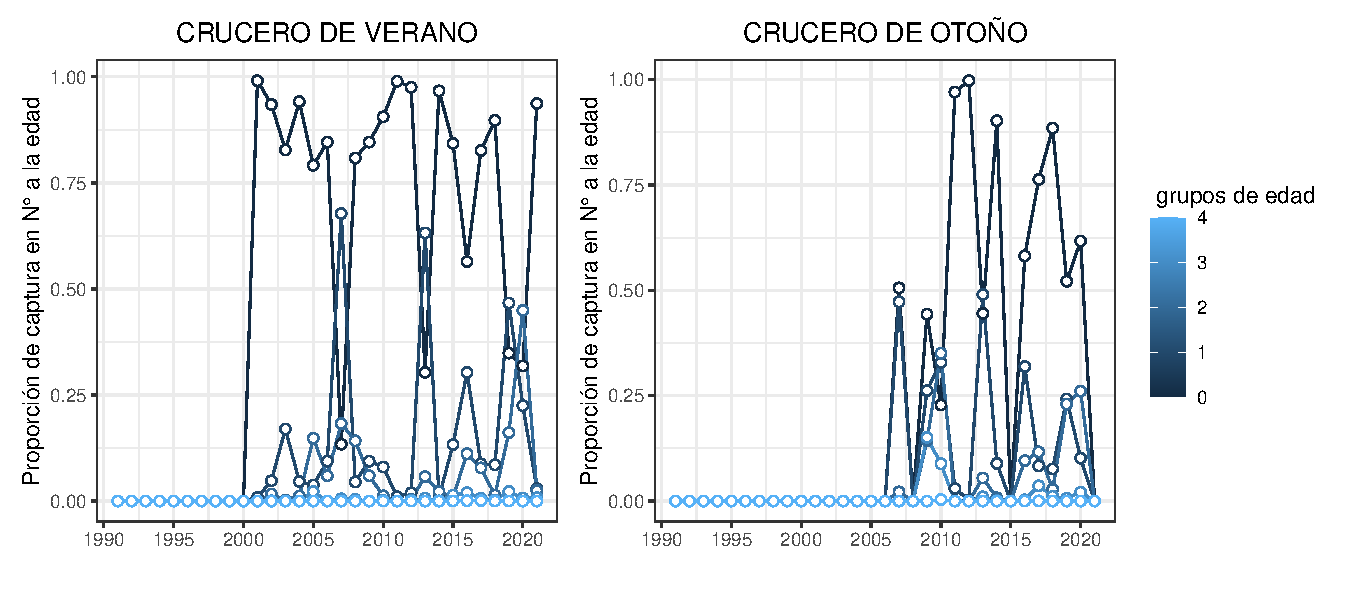
\includegraphics{FigurasInforme_Marzo/F23_datComp-1} \end{center}

\vspace{-0.5cm}
\small

\textbf{Figura 23}. Variabilidad interanual de la proporción de la
captura del crucero de verano (panel izquierdo) y crucero de otoño
(panel derecho) de cada grupo de edad (edad 0 a 4). \normalsize

\begin{center}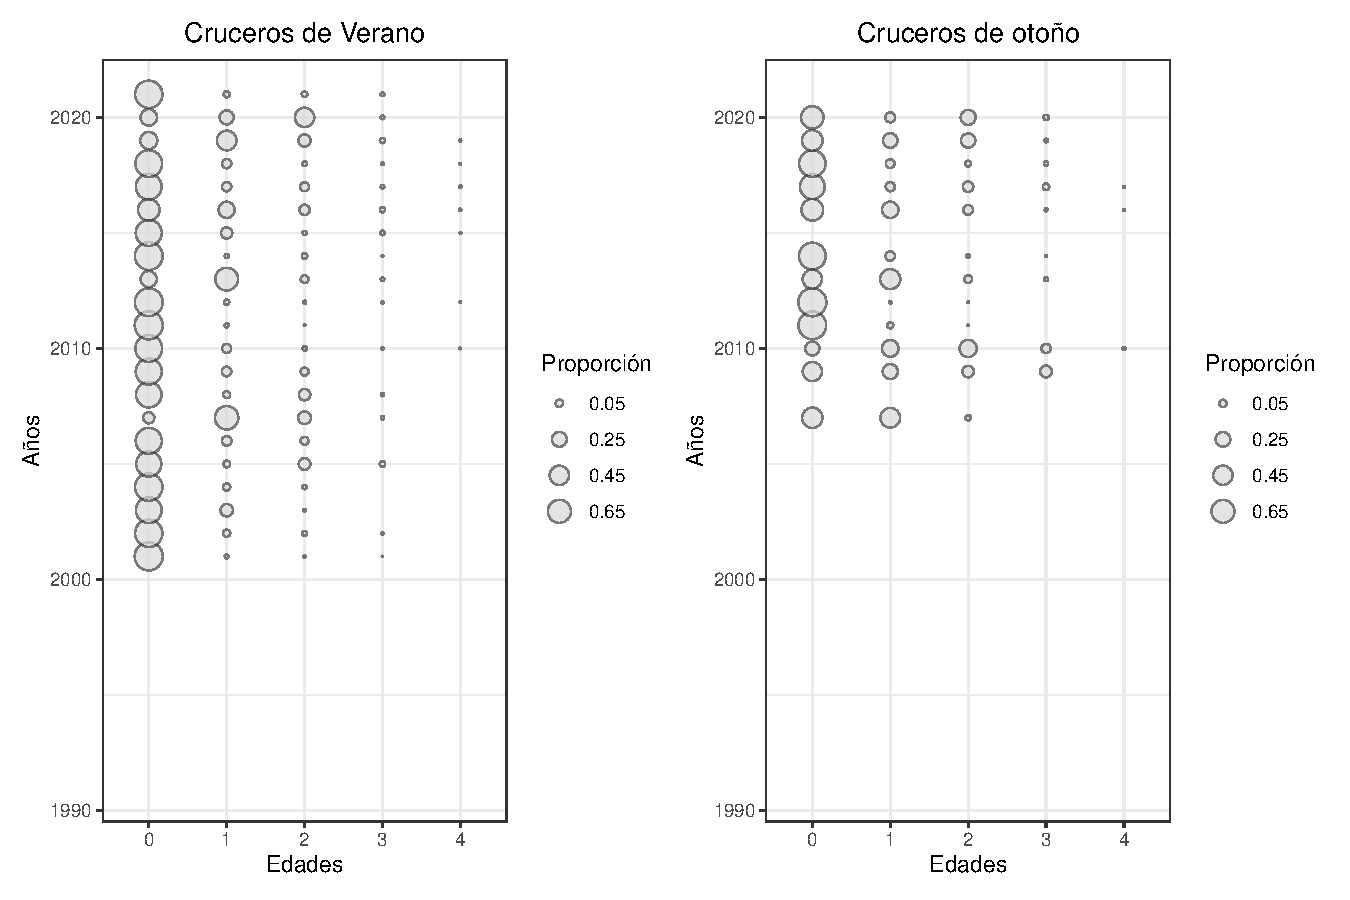
\includegraphics{FigurasInforme_Marzo/Fig24_datComp-1} \end{center}

\vspace{-0.5cm}
\small

\textbf{Figura 24}. Composición de edad de la captura de los cruceros de
verano (panel izquierdo) y otoño (panel derecho) utilizados en la
evaluación de stock . \vspace{0.5cm} \normalsize

\underline{Madurez sexual}

La talla media de madurez sexual se estima considerando el criterio de
50\% de ejemplares maduros, ya que se acepta que la madurez progresa con
la talla o la edad de acuerdo a un modelo logístico de la forma:

\vspace{0.5cm}
\Large
\begin{center} 
$P(l)=\frac{1}{1+exp(\beta_0 + \beta_1*l)}$
\end{center}
\vspace{0.5cm}

\normalsize

Donde P es la proporción de individuos maduros, es la talla (o edad), y
\(\beta_0\) y \(\beta_1\) son parámetros de posición y pendiente,
respectivamente. La talla media de madurez ha sido estimada por varios
autores para sardina común y los parámetros se resumen en la
\textbf{Tabla 18}. Se observa que la talla media de madurez fluctúa
entre 10 y 11,5 cm. En términos de la edad, se consideran completamente
maduros a los individuos mayores o iguales a 1 año de edad, mientras que
los individuos de edad 0 se consideran inmaduros dado que a esa edad la
madurez es menor del 4\%.

Aranís \emph{et al}. (2006) estimaron una talla media de madurez en 11,5
cm LT cuando los virginales son cercanos al 0\% y la maduración
incipiente es casi un 90\% de hembras maduras. La talla media de madurez
(TMM) que es finalmente utilizada como referencia en la evaluación de
stock es la reportada por Aranís \emph{et al}. (2006) (\textbf{Figura
25}). \vspace{0.5cm}

\pagebreak

\small
\begin{center} 
\textbf{Tabla 18.}
\end{center}
\begin{center} 
\vspace{-0.2cm} Parámetros para la ojiva de madurez de sardina común, reportado por varios autores.
\end{center}
\vspace{-0.2cm}

\begin{table}[h]
  \centering
  \resizebox{13cm}{!} {
  \begin{tabular}{|c|c|c|l|l|}
  \hline
 Parámetro     & Pendiente   & Talla media de  &                    &                \\ 
 de posición   & $\beta_1$   &  madurez        & Método             & Fuente         \\ 
 $\beta_0$     &             & $L_{50\%}$ (cm) &                    &    \\ \hline 
               &             & 11              & EMS Macroscópicos  & Arrizaga (1981)            \\
               &             & 10              & Histología         & Mujica y Rojas (1984)      \\
               &             & 11                & IGS                & Cubillos y Arancibia (1993)\\
 11,6            & -1,05         & 11              & EMS macroscópicos  & Arancibia  \textit{et al}. (1994) \\
 20,32         & -2,05       & 10                & EMS macroscópicos  & Cubillos \textit{et al}. (1999)  \\
               &             & 11,5            & EMS macroscópicos  & Aranís \textit{et al}. (2005)    \\
 18,442        & -1,644      & 11,2            & Histología         & Cubillos \textit{et al}. (2009)  \\ \hline
  \end{tabular}}
    \end{table}

\vspace{0.5cm}

\begin{center}
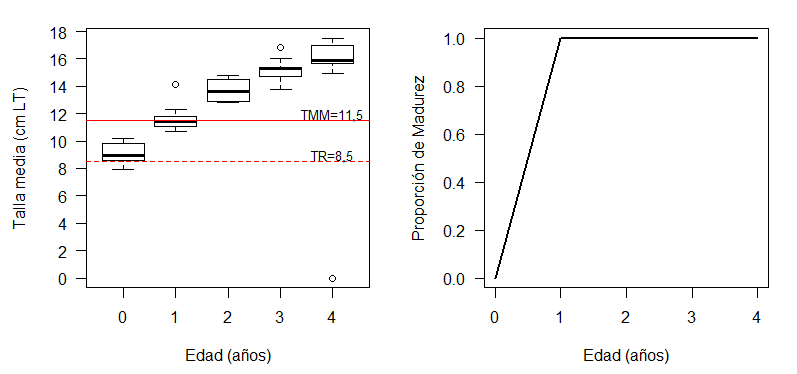
\includegraphics[width=0.75\textwidth]{FigurasInforme_Marzo/Fig26_datosParametros.png}
\end{center}

\small

\textbf{Figura 25}. Talla media a la edad estimada en las claves
talla-edad de las capturas para el período 2001-2015 (TMM= talla media
de madurez y TR=Talla media de reclutamiento) y Ojiva de madurez a la
edad de sardina común. \vspace{0.5cm} \normalsize

\underline{Mortalidad natural (M)}

Respecto de las estimaciones de tasas de mortalidad natural de este
recurso, Canales \emph{et al}. (2007) realiza una revisión de las
estimaciones indirectas de M y cuyos límites están entre M=0,85
año\textsuperscript{-1} (Cubillos \& Arancibia 1993) y M=1,2
año\textsuperscript{-1} (Barría 2001) (\textbf{Tabla 19}).

Para propósitos de evaluación de stock se había estado empleando 1,2
como valor de referencia constante de M entre años y edades. Al
respecto, en el reporte de la revisión por pares de sardina común se
sugiere utilizar un rango de valores fijos de M, ampliando el rango de
estimaciones directas y el valor estimado a partir del modelo y de esta
forma crear un caso base de un set integrado de posibles valores de M.
Por consiguiente, se probaron tres escenarios con M=1,2
año\textsuperscript{-1}, M=0,85 año\textsuperscript{-1}, M=1,0
año\textsuperscript{-1} y M=estimado por el modelo. En base a estos
resultados, se está trabajando con el valor aproximado de M=1,0
año\textsuperscript{-1} para el caso base actual el cual representa una
condición intermedia entre los escenarios analizados y un menor impacto
a nivel de CBA. \vspace{0.5cm}

\small
\begin{center} 
\textbf{Tabla 19.}
\end{center}
\begin{center} 
\vspace{-0.2cm} Estimaciones de mortalidad natural para la sardina común centro-sur (Canales \textit{et al}. 2007).
\end{center}
\vspace{-0.2cm}

\begin{table}[h]
  \centering
  \resizebox{16cm}{!} {
  \begin{tabular}{|c|c|c|l|l|}
  \hline
Área          & Método                     & M ($año^{-1}$)       & Datos      & Referencia                     \\ \hline
Talcahuano  & Pauly (1980)               & 0,85                 & 1990-1991  & Cubillos \& Arancibia (1993)   \\
VIII Región & Average of several methods & 1,30                 & 1990-1993  & Cubillos \textit{et al}. (1994)   \\  
Talcahuano  & Average weighted           & 0,96  [0,71 - 1,3]   & 1990-1997  & Cubillos \textit{et al}. (1998)   \\
Talcahuano  & Hoening (1983)             & 1,2 [0,50 - 2,39]    &            & Barría \textit{et al}. (2001)     \\ \hline
  \end{tabular}}
    \end{table}

\normalsize

\pagebreak

\hypertarget{diagnuxf3stico-del-modelo-de-evaluaciuxf3n-de-stock-1}{%
\subsubsection{4.1.2. Diagnóstico del modelo de evaluación de
stock}\label{diagnuxf3stico-del-modelo-de-evaluaciuxf3n-de-stock-1}}

\hypertarget{ajuste-del-modelo-a-los-datos-y-anuxe1lisis-de-residuos}{%
\paragraph{Ajuste del modelo a los datos y análisis de
residuos}\label{ajuste-del-modelo-a-los-datos-y-anuxe1lisis-de-residuos}}

\quad

Los índices de abundancia de los cruceros acústicos de verano y otoño
contienen un importante nivel de variabilidad que se resume en la
amplitud de los intervalos de confianza supuestos con coeficiente de
variación cv=0,3. El modelo reproduce la tendencia general de la
variabilidad en los niveles de biomasa que han presentado las
estimaciones de cruceros, siendo los valores más altos los que se
escapan del ajuste, lo cual es consistente con la distribución de
probabilidades empleada log-normal que considera sesgo positivo en su
distribución. La \textbf{Figura 26} muestra que a partir del 2014 el
modelo ajusta muy bien la señal de los cruceros acústicos de verano y
otoño.

\begin{center}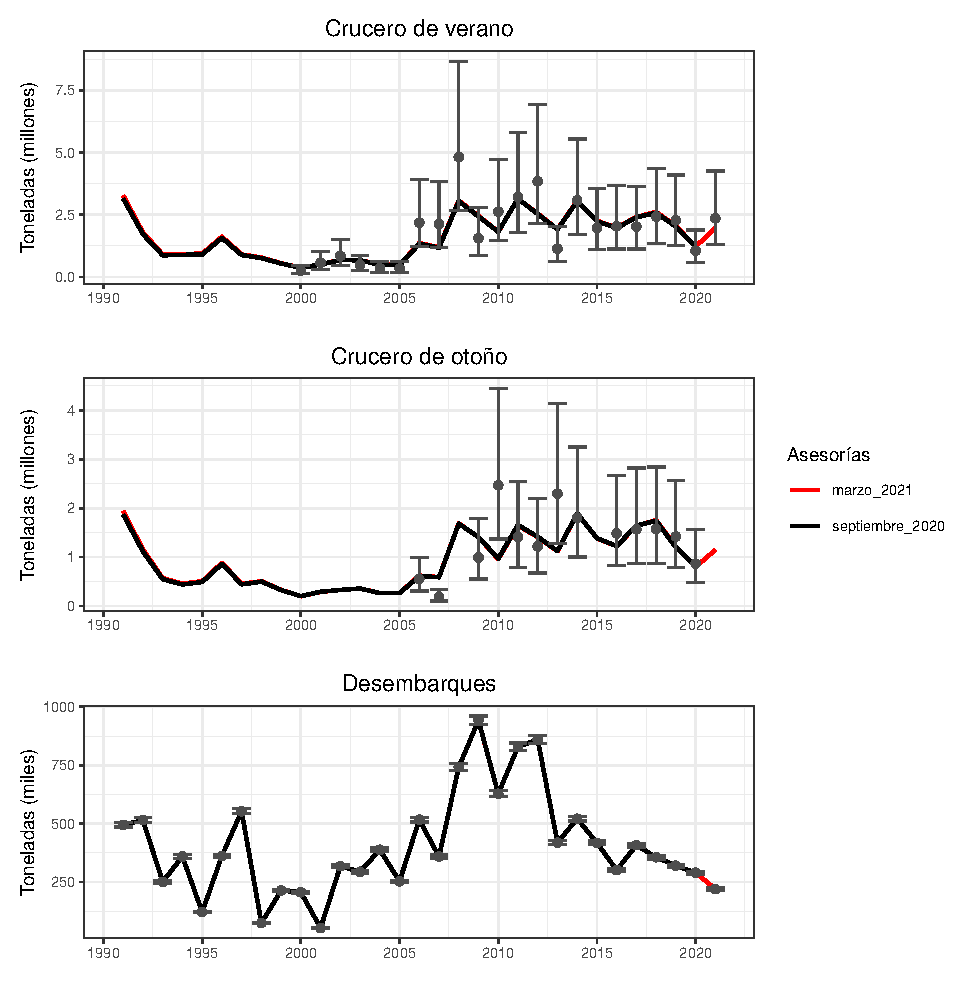
\includegraphics{FigurasInforme_Marzo/Fig26_Ajustes_indices-1} \end{center}

\vspace{-0.5cm}
\small

\textbf{Figura 26}. Ajustes del modelo anual en edades a los valores de
biomasas de cruceros de verano, otoño y desembarques. Las barras
corresponden al intervalo de confianza asintótico y el círculo al valor
del estimador central. Los años de la serie de desembarques corresponden
a año biológico. \vspace{0.5cm} \normalsize

Se destaca que mientras por una parte los residuales del modelo no
sugieren tendencias, es decir, la varianza residual es relativamente
constante y homogénea entre años, el diagrama QQ indica que en términos
generales la linealidad en la escala log se verifica en todos los
índices. Sin perjuicio de esto, la serie de cruceros de verano son los
que tienen mayor variabilidad y lejanía relativa respecto de la línea
esperada (\textbf{Figura 27}). Los datos observados de captura
(desembarques) se asumen insesgados y precisos con un CV de residuos de
0,01 lo cual se refleja en un buen ajuste del modelo a los datos
observados.

\begin{center}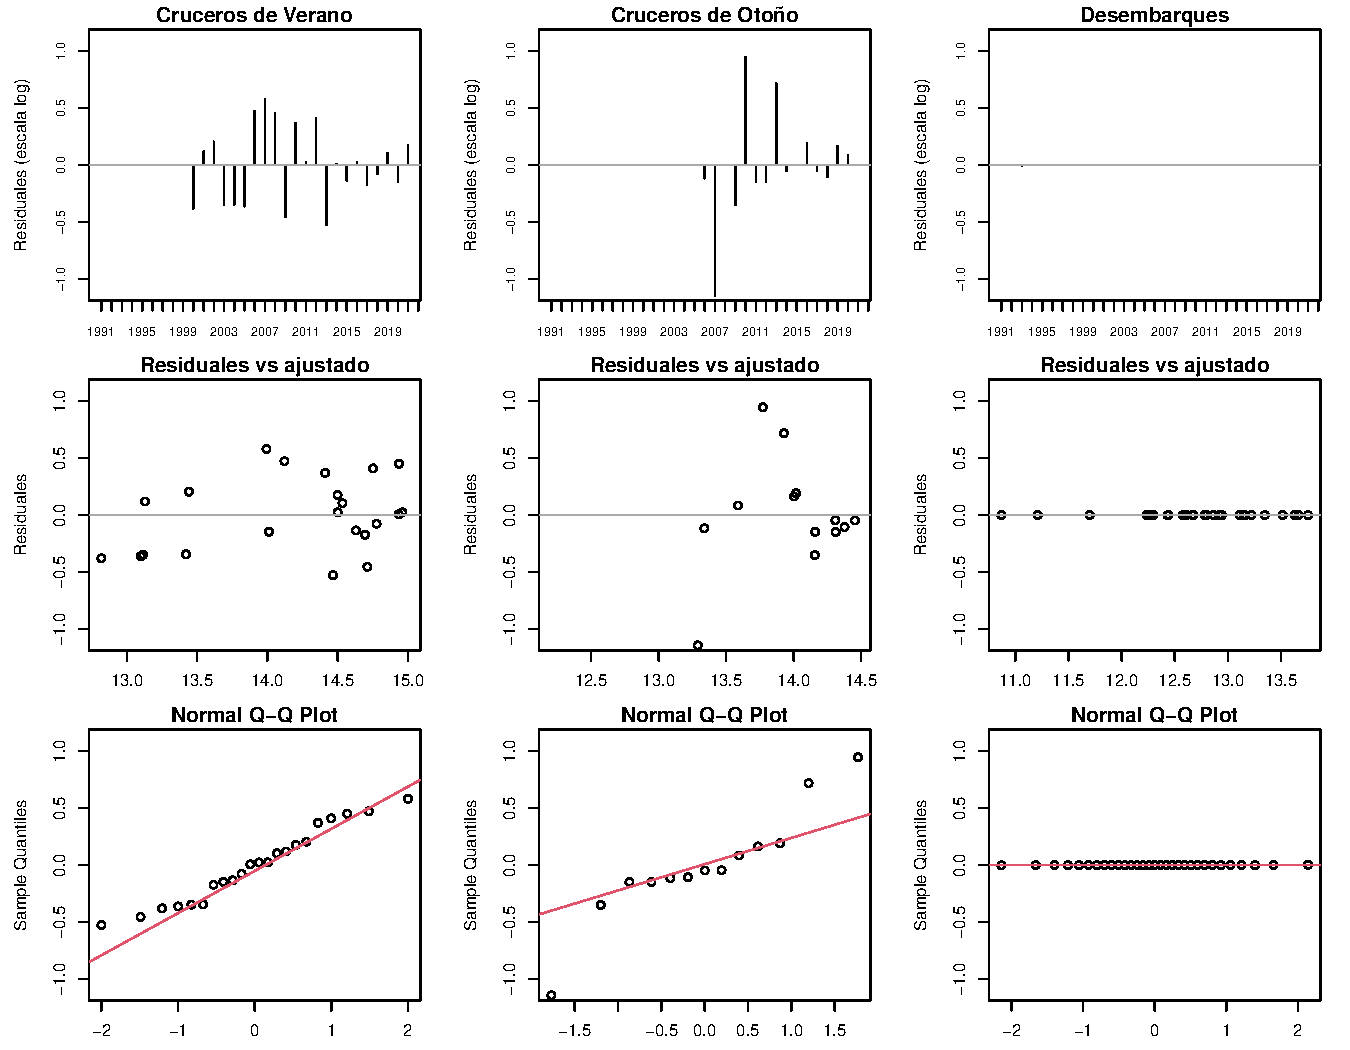
\includegraphics{FigurasInforme_Marzo/Fig27_ajusteBcruReclas-1} \end{center}

\vspace{-0.5cm}
\small

\textbf{Figura 27}. Residuales (escala log) del ajuste del modelo base
actual a los datos observados. \vspace{0.5cm} \normalsize

\pagebreak

\hypertarget{composiciuxf3n-de-edad}{%
\paragraph{Composición de edad}\label{composiciuxf3n-de-edad}}

\quad

El ajuste del modelo a la información de composición de edades en
general presenta un buen desempeño, particularmente en representar de
mejor forma la composición de edades de los cruceros de verano
(\textbf{Figura 28}, \textbf{29} y \textbf{30}). El supuesto de
invariabilidad anual de los patrones de explotación como medida de
parsimonia, genera algunos desajustes en las composiciones de edades de
las capturas, principalmente al inicio de la serie histórica y grupo de
edad 0.

\begin{center}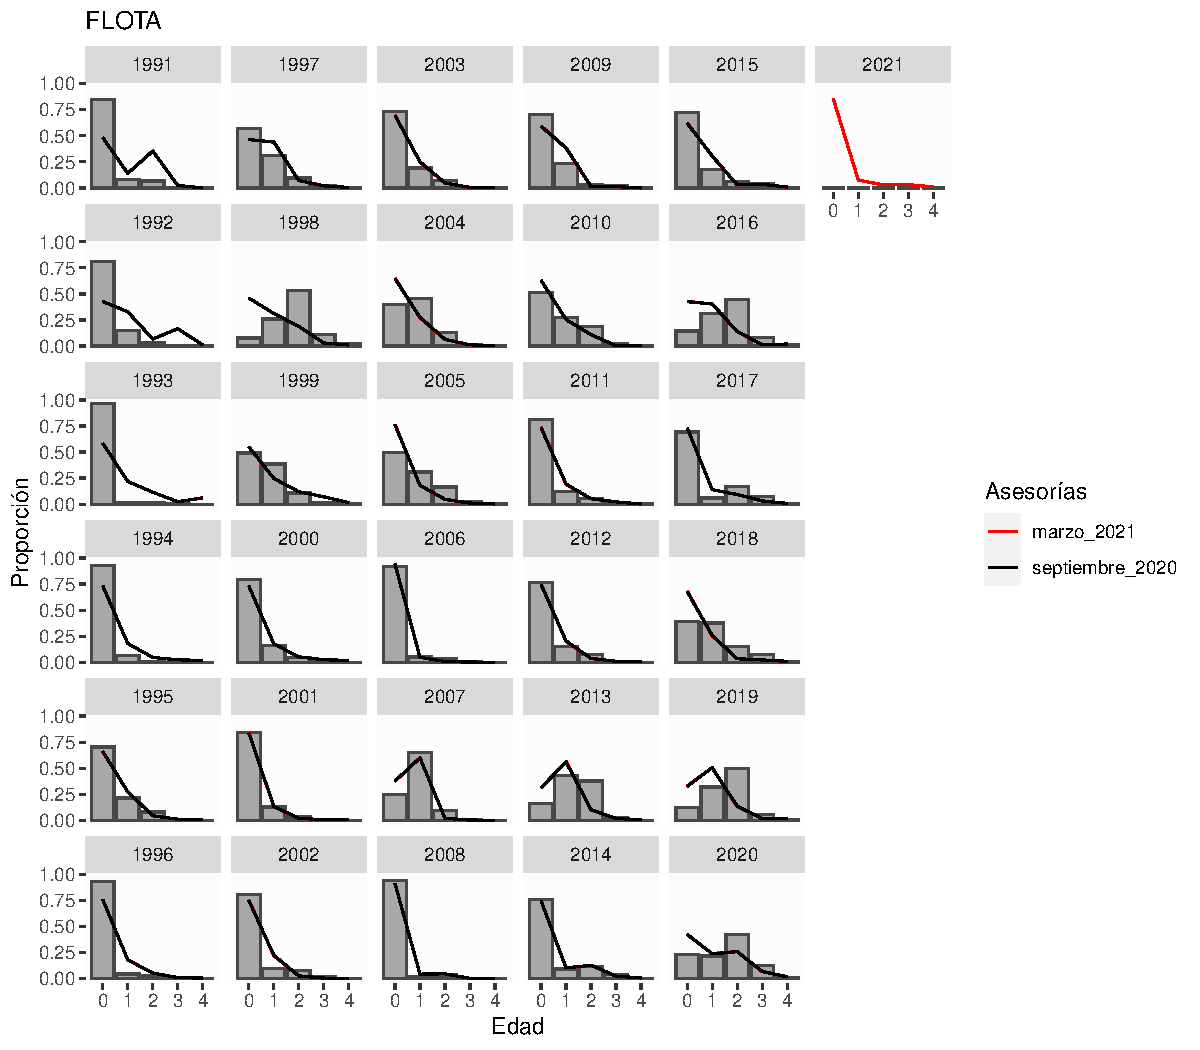
\includegraphics{FigurasInforme_Marzo/Fig28_ajustesCompF-1} \end{center}

\vspace{-0.5cm}
\small

\textbf{Figura 28}. Ajuste del modelo base a las composiciones de edades
de la flota de sardina común de las Regiones de Valparaíso a Los Lagos.
Los años corresponden a año biológico. \vspace{0.3cm} \normalsize

\begin{center}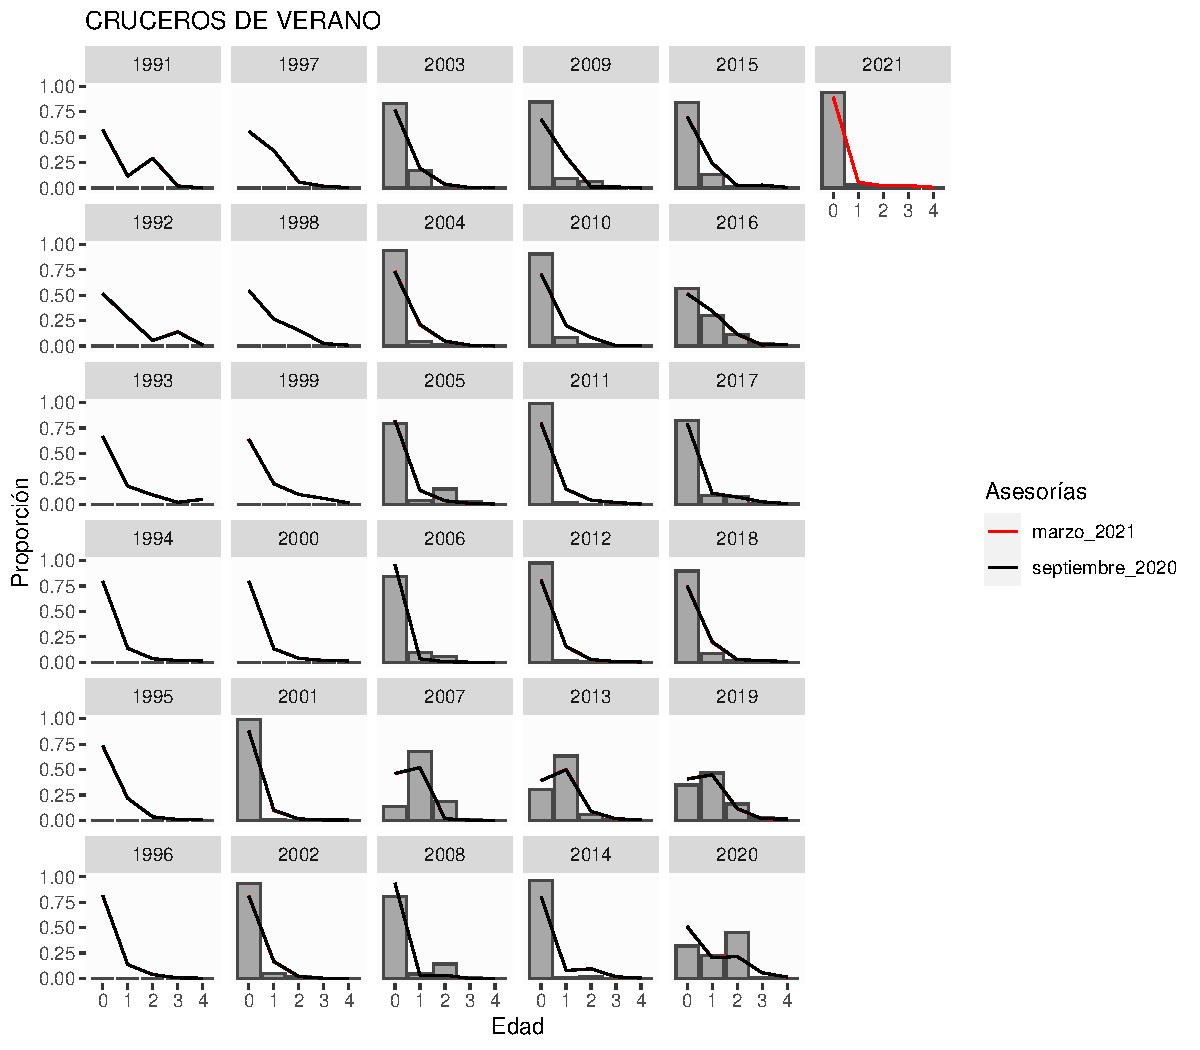
\includegraphics{FigurasInforme_Marzo/Fig29_ajustesCompR-1} \end{center}

\vspace{-0.5cm}
\small

\textbf{Figura 29}. Ajuste del modelo base a las composiciones de edades
de los Cruceros de verano de sardina común de las Regiones de Valparaíso
a Los Lagos. \vspace{0.3cm} \normalsize

\begin{center}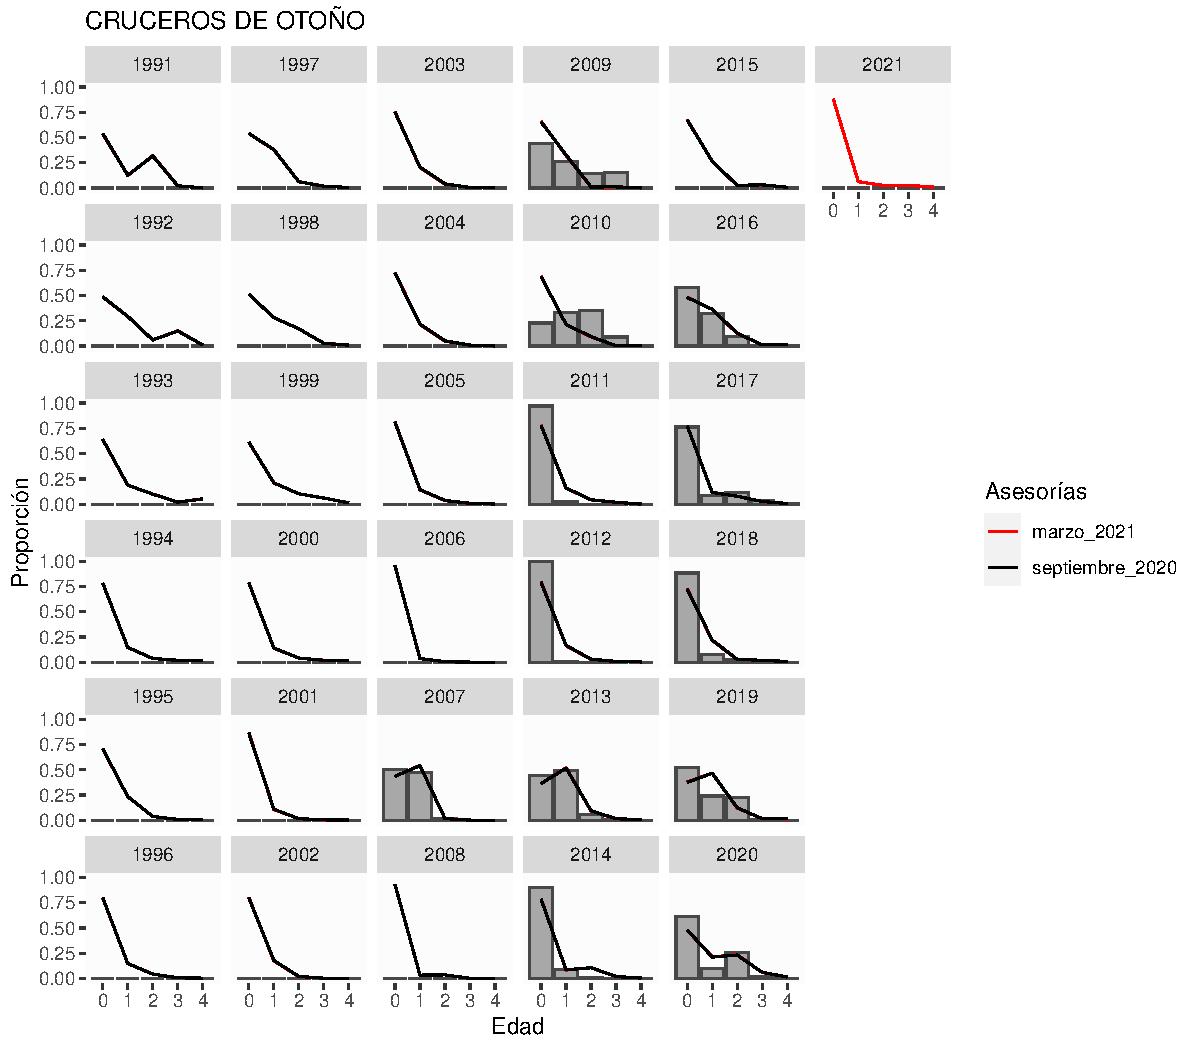
\includegraphics{FigurasInforme_Marzo/Fig30_ajustesCompP-1} \end{center}

\vspace{-0.5cm}
\small

\textbf{Figura 30}. Ajuste del modelo base a las composiciones de edades
de los Cruceros de otoño de sardina común de las Regiones de Valparaíso
a Los Lagos. \vspace{0.3cm} \normalsize

\pagebreak

El comportamiento de los residuales de las composiciones de edades de
los cruceros sugiere ciertos patrones que se reflejan principalmente en
una tendencia a la subestimación de los grupos de edad 0 en los cruceros
de verano. Cabe señalar que en el modelo los datos de composición de
edad de los cruceros de verano y otoño ingresan con un menor peso
estadístico respecto de las composiciones de edades de las capturas de
la flota (menor tamaño de muestra), situación que explicaría entonces
una menor bondad de ajuste y por ende la existencia de tendencias en
algunos residuales (\textbf{Figura 31}).

\begin{center}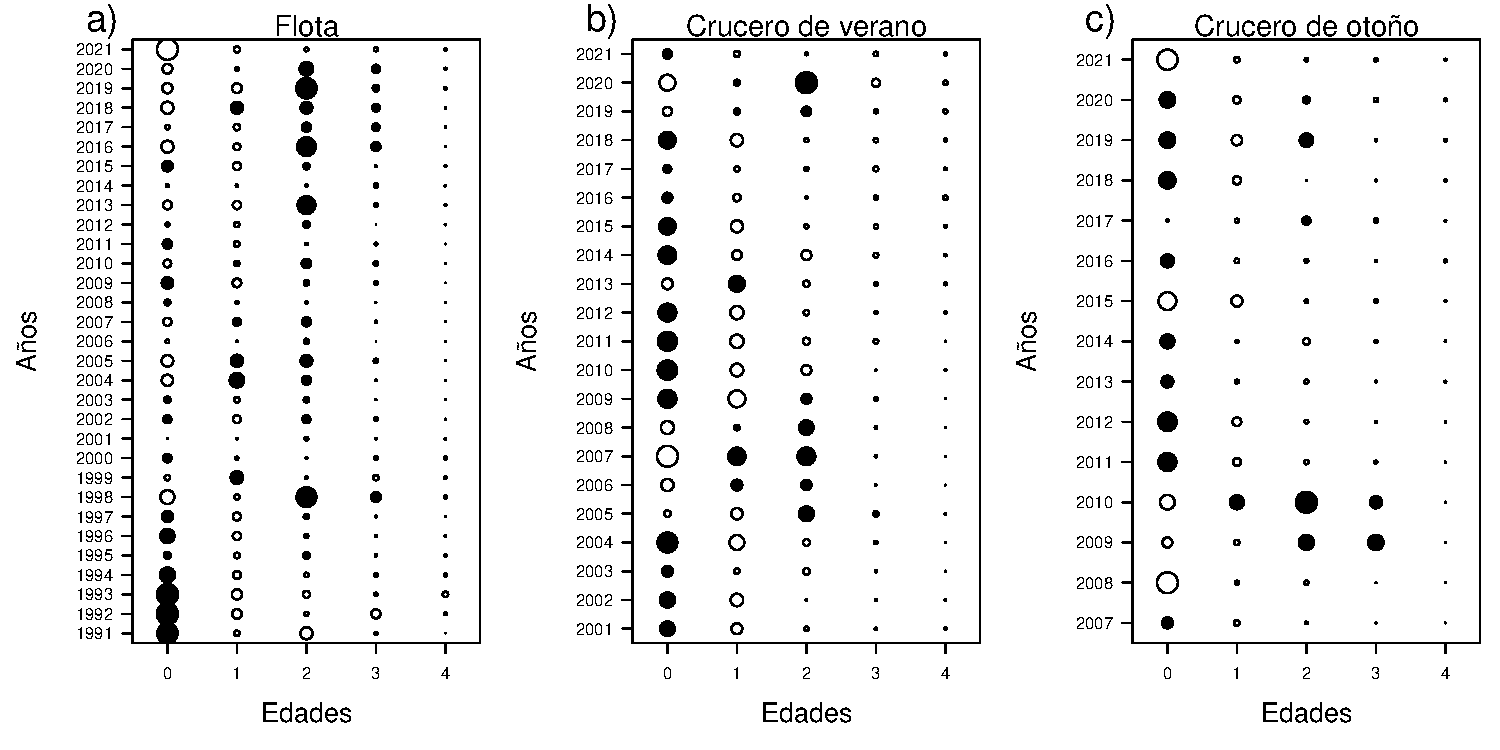
\includegraphics{FigurasInforme_Marzo/Fig31_resComp-1} \end{center}

\vspace{-0.5cm}
\small

\textbf{Figura 31}. Residuales del modelo base actual a las
composiciones de edades de la flota y cruceros. Subestimaciones
(círculos negros) y sobreestimaciones (circulo blanco), donde el tamaño
corresponde a la magnitud relativa de error por edad. \vspace{0.3cm}
\normalsize

\pagebreak

\hypertarget{comparaciuxf3n-con-evaluaciones-anteriores-1}{%
\paragraph{Comparación con evaluaciones
anteriores}\label{comparaciuxf3n-con-evaluaciones-anteriores-1}}

\quad

Se comparan los resultados de los principales indicadores de estatus del
modelo base actual (marzo 2021: MAE0321), con versiones anteriores (sept
2020, julio 2020, marzo 2020, sept 2019) para evaluar la consistencia de
la evaluación presente (\textbf{Figura 32}). Al respecto, el análisis
muestra mayor incertidumbre en los tres últimos años de las series, con
una tendencia a subestimar los niveles de biomasa desovante y
sobre-estimar los niveles de mortalidad por pesca, no obstante, las
diferencias no son significativas.

\begin{center}\includegraphics{FigurasInforme_Marzo/F32_comparación_marzo-1} \end{center}

\small

\textbf{Figura 32}. Comparación con asesorías anteriores del
reclutamiento, biomasa desovante y mortalidad por pesca (F
año\textsuperscript{-1}) de la sardina común. Los años en el eje x
corresponden a año biológico. \vspace{0.5cm} \normalsize

\pagebreak

\hypertarget{anuxe1lisis-retrospectivo-1}{%
\paragraph{Análisis retrospectivo}\label{anuxe1lisis-retrospectivo-1}}

\quad

En la \textbf{Figura 33} se muestra el patrón retrospectivo estándar y
relativo de los reclutas, biomasa desovante y de la mortalidad por pesca
de sardina común para el caso base de marzo 2021 (MAE0321). El análisis
retrospectivo del modelo de evaluación muestra que en términos de rho
(promedio de anomalías retrospectivas) la reducción de información
genera un patrón de subestimación de los reclutas y de la biomasa
desovante (rho = -0,08 y rho = -0,01, respectivamente), con una
sobreestimación de la mortalidad por pesca (rho = +0,04). En general,
los últimos años de las series pueden variar sustancialmente entre las
sucesivas actualizaciones, mientras que hacia los primeros años tienden
a converger a valores estables. La varianza estadística de las variables
utilizadas para medidas de manejo tiende a aumentar en los últimos años
de la serie, por lo tanto, son considerados estimaciones menos
confiables.

\begin{center}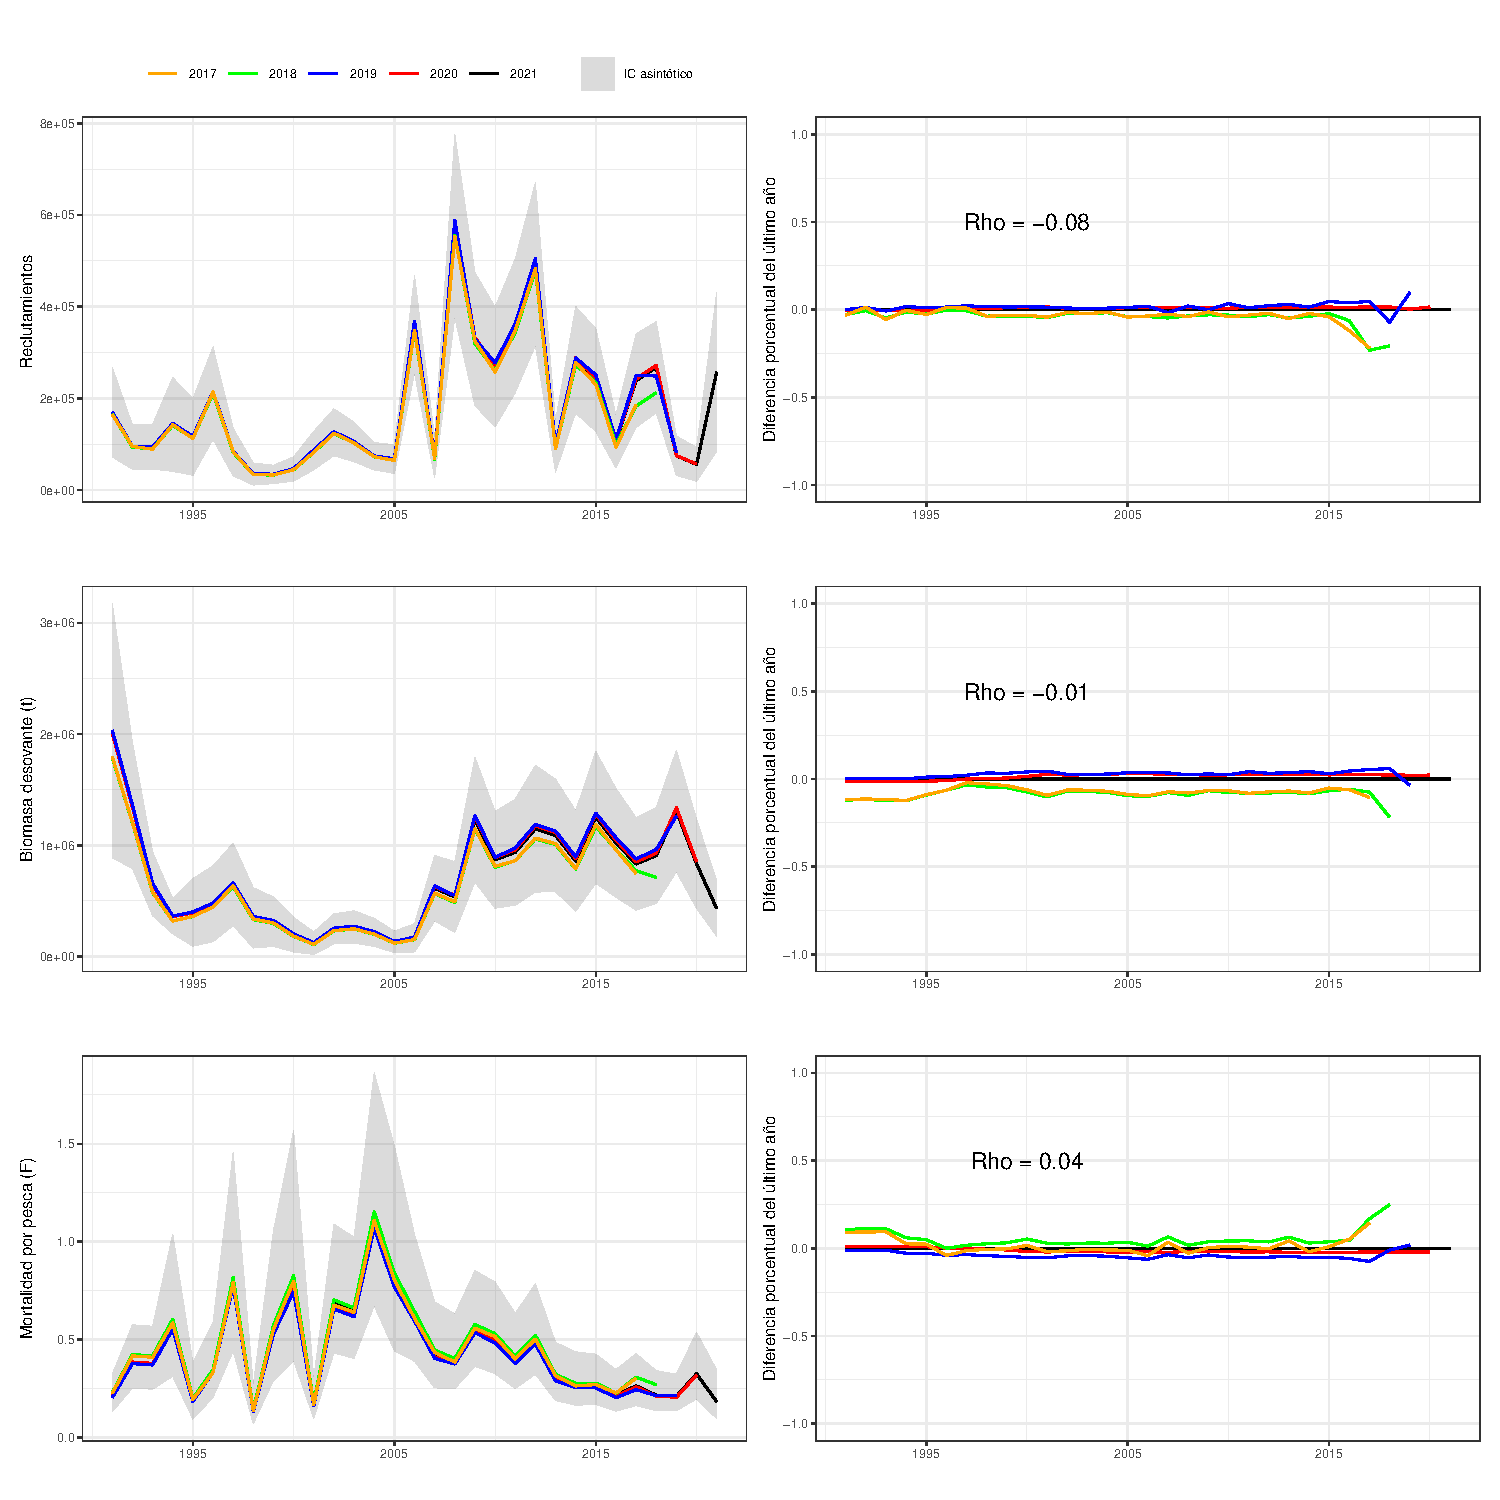
\includegraphics{FigurasInforme_Marzo/F33_retrospectivo_marzo-1} \end{center}

\vspace{-0.5cm}
\small

\textbf{Figura 33}. Patrón retrospectivo estándar (panel izquierdo) y
relativo (panel derecho) de los reclutamientos, biomasa desovante y de
la mortalidad por pesca de sardina común centro-sur para el modelo base
actual. Los años en el eje x corresponden a año biológico. \normalsize

\pagebreak

\hypertarget{perfil-de-verosimilitud}{%
\paragraph{Perfil de verosimilitud}\label{perfil-de-verosimilitud}}

\quad

La \textbf{Figura 34} muestra el perfil de verosimilitud realizado para
la asesoría de marzo 2021 de cada fuente de dato cuyo mínimo representa
la estimación máxima a posteriori del reclutamiento medio (\(R_0\)) para
cada fuente de error del caso base. El perfil muestran que los datos
cuyos perfiles estuvieron más próximos entre si y la diferencia del log
verosimilitud respecto del mínimo se elevó por sobre el criterio
estadístico \(X^2=1,92\) fueron la biomasa acústica de verano (Reclas),
la proporción de edad del crucero de verano (propRecl). Mientras que, el
dato proveniente de los cruceros acústicos de otoño no estaría aportando
información relevante para la definición del reclutamiento medio.

\begin{center}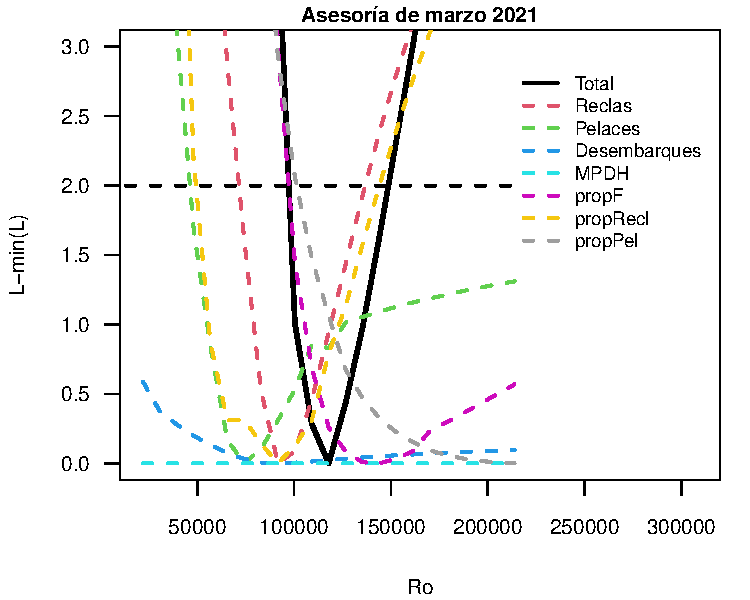
\includegraphics{FigurasInforme_Marzo/F34_verosimilitud_marz-1} \end{center}

\vspace{-0.5cm}
\small

\textbf{Figura 34}. Perfiles de verosimilitud donde la línea horizontal
representa el nivel crítico para el test \(\chi^2\). \vspace{0.5cm}
\normalsize

\pagebreak

\hypertarget{objetivo-especuxedfico-2-1}{%
\subsection{4.2. Objetivo específico
2:}\label{objetivo-especuxedfico-2-1}}

\vspace{-0.2cm}

\emph{``Establecer el estatus actualizado de sardina común, sobre la
base de sus principales indicadores estandarizados de estado y flujo,
propagando para estos efectos todas las fuentes de incertidumbre
subyacente a la pesquería.''}

\hypertarget{indicadores-del-stock}{%
\subsubsection{4.2.1. Indicadores del
stock}\label{indicadores-del-stock}}

\hypertarget{reclutamientos}{%
\paragraph{Reclutamientos:}\label{reclutamientos}}

Las tendencias de los reclutamientos han mostrado importantes
fluctuaciones interanuales y en su historia conocida se aprecian tres
períodos relevantes, a) Reclutamiento promedio del período 1991-2007 con
los niveles más bajos de reclutamientos (113 mil millones de peces), b)
Reclutamiento promedio del período 2008-2012 con los más altos niveles
de reclutamiento (405 mil millones de peces) y c) Reclutamiento promedio
del período 2013-2021 en torno a 180 mil millones de peces. En relación
a los tres períodos relevantes, el reclutamiento 2021 es un 128\% mayor
al Reclutamiento bajo (período 1991-2007), un 36\% menor al
Reclutamiento alto (período 2008-2012) y un 43\% mayor al Reclutamiento
medio (2013-2021) (\textbf{Tabla 20} y \textbf{Figura 35}).

\hypertarget{biomasa-total-y-desovante}{%
\paragraph{Biomasa total y desovante:}\label{biomasa-total-y-desovante}}

La biomasa total de este recurso, es sustentada esencialmente en los
grupos de edad 0 y 1 año. En general, los grupos de edad 2+ no revisten
mayor contribución en la producción tanto a nivel de desove como de
biomasa disponible a la flota. La tendencia de la biomasa total muestra
un importante crecimiento a partir del año 2008 que genera un cambio de
nivel que se mantiene hasta el 2018. Sin embargo, presenta una alta
variabilidad producto de las fluctuaciones del reclutamiento. El
promedio de la biomasa total para el período de mayor productividad de
sardina común entre los años 2008 y 2012 es de 2,65 millones de
toneladas. Para el año 2021 se estimó una biomasa total de 1,78 millones
de toneladas, un 33\% menor al promedio del período de mayor
productividad y un 10\% mayor al promedio histórico de la serie
(promedio 1991-2021 = 1,62 millones de t.) (\textbf{Tabla 20} y
\textbf{Figura 35}). Por otro lado, la biomasa desovante promedio de la
serie histórica se encuentra en torno a 702 mil toneladas, mientras que
el promedio de los 8 años previos (período 2013-2020) de la serie es de
1,01 millones de toneladas. Al respecto, la biomasa desovante esperada
para el año biológico 2020/2021 es un 39\% menor al promedio histórico y
un 58\% menor al promedio de los 8 años previos (período 2013-2020)
(\textbf{Tabla 20} y \textbf{Figura 35}). La biomasa desovante al Máximo
Rendimiento Sostenido (BD\textsubscript{RMS}) está en torno a las 801
mil toneladas, de esta forma la BD\textsubscript{2020/2021} esperada
está un 46\% bajo BD\textsubscript{RMS} (\textbf{Tabla 21 y 22} y
\textbf{Figura 35}). La biomasa desovante está sustentada principalente
por la fracción adulta, correspondiente a individuos de edad 1+, la cual
disminuyó su abundancia producto de la disminución del reclutamiento de
dos años previos consecutivos 2019 y 2020 junto a la disminución de la
biomasa adulta (1+ años) el 2020, provocando que la biomasa desovante
del año biológico 2020-21 se reduzca significativamente respecto a años
previos.

\hypertarget{mortalidad-por-pesca}{%
\paragraph{Mortalidad por pesca:}\label{mortalidad-por-pesca}}

La mortalidad por pesca (Ft) ha sido más bien baja, en general menor a
la mortalidad natural (M=1,0 año\textsuperscript{-1}), excepto para el
año 2004 cuando los niveles de biomasa eran bajos. Esto se ve reflejado
en las capturas, que, en promedio, han seguido las fluctuaciones en
biomasa con tasas de explotación moderadas (\textbf{Tabla 20} y
\textbf{Figura 35}). A partir del año 2005, la mortalidad por pesca ha
seguido una tendencia al descenso, acentuada desde el año 2013 bajo el
valor de F\textsubscript{RMS} producto de la aplicación de F60\%. Para
el año 2020/2021 se estima una Ft=0,18 año\textsuperscript{-1}, un 39\%
bajo F\textsubscript{RMS}, no obstante, este valor se debe considerar
preliminar ya que está basado en un supuesto de captura 2020/21
(\textbf{Tabla 21 y 22} y \textbf{Figura 35}).

\hypertarget{selectividades}{%
\paragraph{Selectividades:}\label{selectividades}}

Por su parte, las selectividades de la flota y cruceros de otoño indican
que el recurso alcanza su completo reclutamiento a la pesquería a la
edad de 1 año cuando su retención es del 100\% aprox., mientras que los
individuos de edad 0 (reclutamientos) son vulnerados entre 70\% (flota)
y 84\% (crucero de otoño). De igual forma, la información del crucero
acústico de verano indica que todos los individuos son vulnerables en un
100\% por el arte de pesca empleado (arrastre de media-agua y
cubre-copo) y cubiertos por el diseño de muestreo (\textbf{Figura 36}).

\begin{center}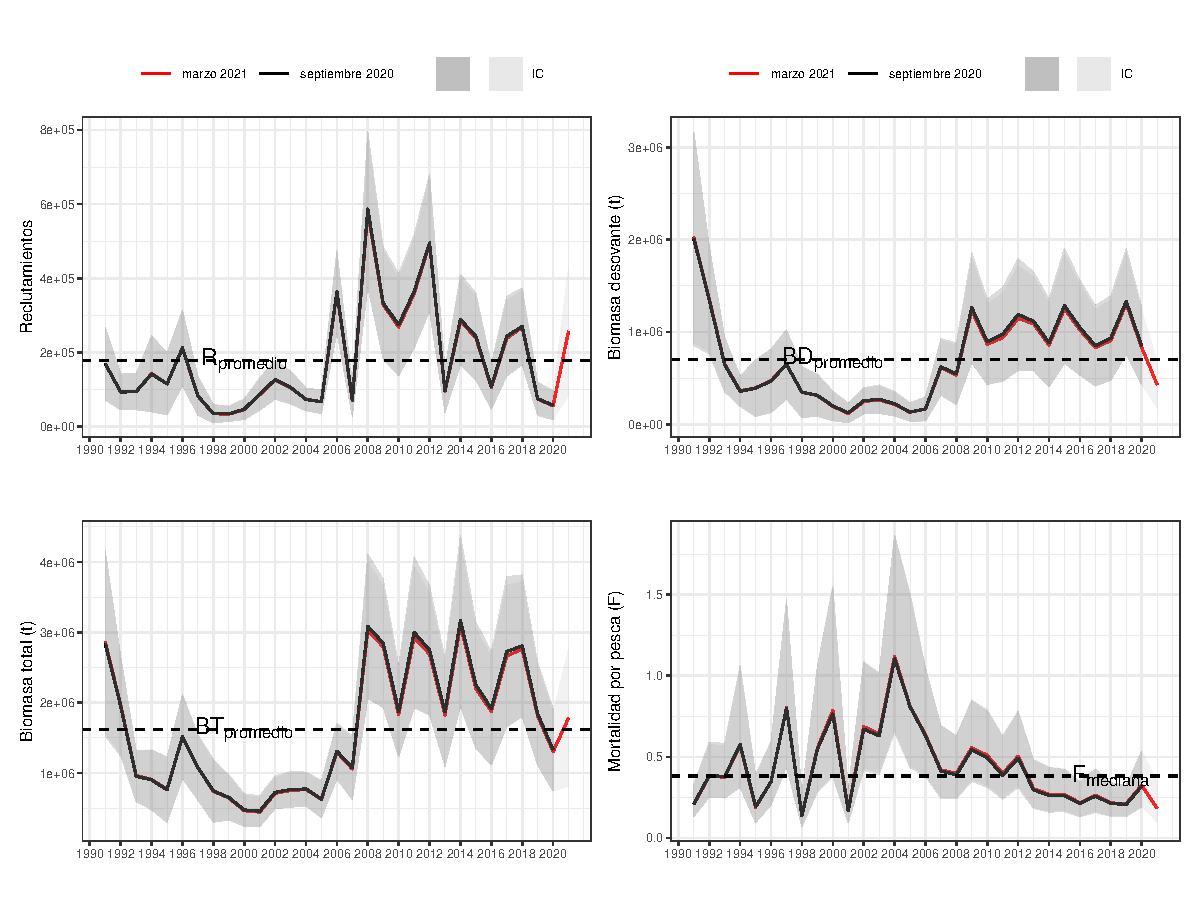
\includegraphics{FigurasInforme_Marzo/F35_Varpobl-1} \end{center}

\vspace{-0.5cm}
\small

\textbf{Figura 35}. Estimaciones medias de los reclutamientos, biomasa
total, biomasa desovante y mortalidad por pesca y su respectivo
Intervalo de Confianza (IC). Las línea segmentada corresponde al
promedio y mediana de la serie respectiva. Los años en el eje x
corresponden a año biológico. \vspace{0.5cm} \normalsize

\pagebreak

\small
\begin{center} 
\textbf{Tabla 20.}
\end{center}
\begin{center} 
\vspace{-0.2cm} Comparación de las variables poblacionales  estimadas en la evaluación de septiembre 2020 y marzo 2021 de sardina común de las Regiones de Valparaíso a Los Lagos.
\end{center}
\vspace{-0.2cm}
\footnotesize

\begin{longtable}[]{@{}lllllllll@{}}
\toprule
\begin{minipage}[b]{0.06\columnwidth}\raggedright
Año\strut
\end{minipage} & \begin{minipage}[b]{0.09\columnwidth}\raggedright
\(BD_{sept}\)\strut
\end{minipage} & \begin{minipage}[b]{0.10\columnwidth}\raggedright
\(BD_{marzo}\)\strut
\end{minipage} & \begin{minipage}[b]{0.09\columnwidth}\raggedright
\(BT_{sept}\)\strut
\end{minipage} & \begin{minipage}[b]{0.10\columnwidth}\raggedright
\(BT_{marzo}\)\strut
\end{minipage} & \begin{minipage}[b]{0.08\columnwidth}\raggedright
\(R_{sept}\)\strut
\end{minipage} & \begin{minipage}[b]{0.09\columnwidth}\raggedright
\(R_{marzo}\)\strut
\end{minipage} & \begin{minipage}[b]{0.08\columnwidth}\raggedright
\(F_{sept}\)\strut
\end{minipage} & \begin{minipage}[b]{0.09\columnwidth}\raggedright
\(F_{marzo}\)\strut
\end{minipage}\tabularnewline
\midrule
\endhead
\begin{minipage}[t]{0.06\columnwidth}\raggedright
1990/91\strut
\end{minipage} & \begin{minipage}[t]{0.09\columnwidth}\raggedright
2008700\strut
\end{minipage} & \begin{minipage}[t]{0.10\columnwidth}\raggedright
2030000\strut
\end{minipage} & \begin{minipage}[t]{0.09\columnwidth}\raggedright
2844200\strut
\end{minipage} & \begin{minipage}[t]{0.10\columnwidth}\raggedright
2870400\strut
\end{minipage} & \begin{minipage}[t]{0.08\columnwidth}\raggedright
169670\strut
\end{minipage} & \begin{minipage}[t]{0.09\columnwidth}\raggedright
170120\strut
\end{minipage} & \begin{minipage}[t]{0.08\columnwidth}\raggedright
0.209\strut
\end{minipage} & \begin{minipage}[t]{0.09\columnwidth}\raggedright
0.207\strut
\end{minipage}\tabularnewline
\begin{minipage}[t]{0.06\columnwidth}\raggedright
1991/92\strut
\end{minipage} & \begin{minipage}[t]{0.09\columnwidth}\raggedright
1344500\strut
\end{minipage} & \begin{minipage}[t]{0.10\columnwidth}\raggedright
1358500\strut
\end{minipage} & \begin{minipage}[t]{0.09\columnwidth}\raggedright
1949500\strut
\end{minipage} & \begin{minipage}[t]{0.10\columnwidth}\raggedright
1966700\strut
\end{minipage} & \begin{minipage}[t]{0.08\columnwidth}\raggedright
93768\strut
\end{minipage} & \begin{minipage}[t]{0.09\columnwidth}\raggedright
94041\strut
\end{minipage} & \begin{minipage}[t]{0.08\columnwidth}\raggedright
0.386\strut
\end{minipage} & \begin{minipage}[t]{0.09\columnwidth}\raggedright
0.382\strut
\end{minipage}\tabularnewline
\begin{minipage}[t]{0.06\columnwidth}\raggedright
1992/93\strut
\end{minipage} & \begin{minipage}[t]{0.09\columnwidth}\raggedright
645250\strut
\end{minipage} & \begin{minipage}[t]{0.10\columnwidth}\raggedright
652550\strut
\end{minipage} & \begin{minipage}[t]{0.09\columnwidth}\raggedright
955290\strut
\end{minipage} & \begin{minipage}[t]{0.10\columnwidth}\raggedright
964360\strut
\end{minipage} & \begin{minipage}[t]{0.08\columnwidth}\raggedright
94409\strut
\end{minipage} & \begin{minipage}[t]{0.09\columnwidth}\raggedright
94707\strut
\end{minipage} & \begin{minipage}[t]{0.08\columnwidth}\raggedright
0.379\strut
\end{minipage} & \begin{minipage}[t]{0.09\columnwidth}\raggedright
0.375\strut
\end{minipage}\tabularnewline
\begin{minipage}[t]{0.06\columnwidth}\raggedright
1993/94\strut
\end{minipage} & \begin{minipage}[t]{0.09\columnwidth}\raggedright
358150\strut
\end{minipage} & \begin{minipage}[t]{0.10\columnwidth}\raggedright
362070\strut
\end{minipage} & \begin{minipage}[t]{0.09\columnwidth}\raggedright
902180\strut
\end{minipage} & \begin{minipage}[t]{0.10\columnwidth}\raggedright
909000\strut
\end{minipage} & \begin{minipage}[t]{0.08\columnwidth}\raggedright
142470\strut
\end{minipage} & \begin{minipage}[t]{0.09\columnwidth}\raggedright
143180\strut
\end{minipage} & \begin{minipage}[t]{0.08\columnwidth}\raggedright
0.576\strut
\end{minipage} & \begin{minipage}[t]{0.09\columnwidth}\raggedright
0.57\strut
\end{minipage}\tabularnewline
\begin{minipage}[t]{0.06\columnwidth}\raggedright
1994/95\strut
\end{minipage} & \begin{minipage}[t]{0.09\columnwidth}\raggedright
390940\strut
\end{minipage} & \begin{minipage}[t]{0.10\columnwidth}\raggedright
395090\strut
\end{minipage} & \begin{minipage}[t]{0.09\columnwidth}\raggedright
761620\strut
\end{minipage} & \begin{minipage}[t]{0.10\columnwidth}\raggedright
767170\strut
\end{minipage} & \begin{minipage}[t]{0.08\columnwidth}\raggedright
115500\strut
\end{minipage} & \begin{minipage}[t]{0.09\columnwidth}\raggedright
115760\strut
\end{minipage} & \begin{minipage}[t]{0.08\columnwidth}\raggedright
0.192\strut
\end{minipage} & \begin{minipage}[t]{0.09\columnwidth}\raggedright
0.19\strut
\end{minipage}\tabularnewline
\begin{minipage}[t]{0.06\columnwidth}\raggedright
1995/96\strut
\end{minipage} & \begin{minipage}[t]{0.09\columnwidth}\raggedright
469770\strut
\end{minipage} & \begin{minipage}[t]{0.10\columnwidth}\raggedright
473120\strut
\end{minipage} & \begin{minipage}[t]{0.09\columnwidth}\raggedright
1518000\strut
\end{minipage} & \begin{minipage}[t]{0.10\columnwidth}\raggedright
1517100\strut
\end{minipage} & \begin{minipage}[t]{0.08\columnwidth}\raggedright
212650\strut
\end{minipage} & \begin{minipage}[t]{0.09\columnwidth}\raggedright
211490\strut
\end{minipage} & \begin{minipage}[t]{0.08\columnwidth}\raggedright
0.347\strut
\end{minipage} & \begin{minipage}[t]{0.09\columnwidth}\raggedright
0.347\strut
\end{minipage}\tabularnewline
\begin{minipage}[t]{0.06\columnwidth}\raggedright
1996/97\strut
\end{minipage} & \begin{minipage}[t]{0.09\columnwidth}\raggedright
648700\strut
\end{minipage} & \begin{minipage}[t]{0.10\columnwidth}\raggedright
647450\strut
\end{minipage} & \begin{minipage}[t]{0.09\columnwidth}\raggedright
1080200\strut
\end{minipage} & \begin{minipage}[t]{0.10\columnwidth}\raggedright
1077600\strut
\end{minipage} & \begin{minipage}[t]{0.08\columnwidth}\raggedright
83311\strut
\end{minipage} & \begin{minipage}[t]{0.09\columnwidth}\raggedright
82828\strut
\end{minipage} & \begin{minipage}[t]{0.08\columnwidth}\raggedright
0.8\strut
\end{minipage} & \begin{minipage}[t]{0.09\columnwidth}\raggedright
0.803\strut
\end{minipage}\tabularnewline
\begin{minipage}[t]{0.06\columnwidth}\raggedright
1997/98\strut
\end{minipage} & \begin{minipage}[t]{0.09\columnwidth}\raggedright
348370\strut
\end{minipage} & \begin{minipage}[t]{0.10\columnwidth}\raggedright
346010\strut
\end{minipage} & \begin{minipage}[t]{0.09\columnwidth}\raggedright
746840\strut
\end{minipage} & \begin{minipage}[t]{0.10\columnwidth}\raggedright
741130\strut
\end{minipage} & \begin{minipage}[t]{0.08\columnwidth}\raggedright
35378\strut
\end{minipage} & \begin{minipage}[t]{0.09\columnwidth}\raggedright
35062\strut
\end{minipage} & \begin{minipage}[t]{0.08\columnwidth}\raggedright
0.137\strut
\end{minipage} & \begin{minipage}[t]{0.09\columnwidth}\raggedright
0.138\strut
\end{minipage}\tabularnewline
\begin{minipage}[t]{0.06\columnwidth}\raggedright
1998/99\strut
\end{minipage} & \begin{minipage}[t]{0.09\columnwidth}\raggedright
314830\strut
\end{minipage} & \begin{minipage}[t]{0.10\columnwidth}\raggedright
311640\strut
\end{minipage} & \begin{minipage}[t]{0.09\columnwidth}\raggedright
653870\strut
\end{minipage} & \begin{minipage}[t]{0.10\columnwidth}\raggedright
646260\strut
\end{minipage} & \begin{minipage}[t]{0.08\columnwidth}\raggedright
34847\strut
\end{minipage} & \begin{minipage}[t]{0.09\columnwidth}\raggedright
34292\strut
\end{minipage} & \begin{minipage}[t]{0.08\columnwidth}\raggedright
0.547\strut
\end{minipage} & \begin{minipage}[t]{0.09\columnwidth}\raggedright
0.555\strut
\end{minipage}\tabularnewline
\begin{minipage}[t]{0.06\columnwidth}\raggedright
1999/00\strut
\end{minipage} & \begin{minipage}[t]{0.09\columnwidth}\raggedright
198580\strut
\end{minipage} & \begin{minipage}[t]{0.10\columnwidth}\raggedright
194090\strut
\end{minipage} & \begin{minipage}[t]{0.09\columnwidth}\raggedright
475590\strut
\end{minipage} & \begin{minipage}[t]{0.10\columnwidth}\raggedright
465230\strut
\end{minipage} & \begin{minipage}[t]{0.08\columnwidth}\raggedright
47251\strut
\end{minipage} & \begin{minipage}[t]{0.09\columnwidth}\raggedright
46073\strut
\end{minipage} & \begin{minipage}[t]{0.08\columnwidth}\raggedright
0.764\strut
\end{minipage} & \begin{minipage}[t]{0.09\columnwidth}\raggedright
0.786\strut
\end{minipage}\tabularnewline
\begin{minipage}[t]{0.06\columnwidth}\raggedright
2000/01\strut
\end{minipage} & \begin{minipage}[t]{0.09\columnwidth}\raggedright
123590\strut
\end{minipage} & \begin{minipage}[t]{0.10\columnwidth}\raggedright
118470\strut
\end{minipage} & \begin{minipage}[t]{0.09\columnwidth}\raggedright
457800\strut
\end{minipage} & \begin{minipage}[t]{0.10\columnwidth}\raggedright
444970\strut
\end{minipage} & \begin{minipage}[t]{0.08\columnwidth}\raggedright
88252\strut
\end{minipage} & \begin{minipage}[t]{0.09\columnwidth}\raggedright
86319\strut
\end{minipage} & \begin{minipage}[t]{0.08\columnwidth}\raggedright
0.167\strut
\end{minipage} & \begin{minipage}[t]{0.09\columnwidth}\raggedright
0.172\strut
\end{minipage}\tabularnewline
\begin{minipage}[t]{0.06\columnwidth}\raggedright
2001/02\strut
\end{minipage} & \begin{minipage}[t]{0.09\columnwidth}\raggedright
254560\strut
\end{minipage} & \begin{minipage}[t]{0.10\columnwidth}\raggedright
246340\strut
\end{minipage} & \begin{minipage}[t]{0.09\columnwidth}\raggedright
725490\strut
\end{minipage} & \begin{minipage}[t]{0.10\columnwidth}\raggedright
713020\strut
\end{minipage} & \begin{minipage}[t]{0.08\columnwidth}\raggedright
126940\strut
\end{minipage} & \begin{minipage}[t]{0.09\columnwidth}\raggedright
126130\strut
\end{minipage} & \begin{minipage}[t]{0.08\columnwidth}\raggedright
0.671\strut
\end{minipage} & \begin{minipage}[t]{0.09\columnwidth}\raggedright
0.686\strut
\end{minipage}\tabularnewline
\begin{minipage}[t]{0.06\columnwidth}\raggedright
2002/03\strut
\end{minipage} & \begin{minipage}[t]{0.09\columnwidth}\raggedright
272510\strut
\end{minipage} & \begin{minipage}[t]{0.10\columnwidth}\raggedright
264590\strut
\end{minipage} & \begin{minipage}[t]{0.09\columnwidth}\raggedright
766550\strut
\end{minipage} & \begin{minipage}[t]{0.10\columnwidth}\raggedright
753550\strut
\end{minipage} & \begin{minipage}[t]{0.08\columnwidth}\raggedright
105990\strut
\end{minipage} & \begin{minipage}[t]{0.09\columnwidth}\raggedright
105110\strut
\end{minipage} & \begin{minipage}[t]{0.08\columnwidth}\raggedright
0.63\strut
\end{minipage} & \begin{minipage}[t]{0.09\columnwidth}\raggedright
0.643\strut
\end{minipage}\tabularnewline
\begin{minipage}[t]{0.06\columnwidth}\raggedright
2003/04\strut
\end{minipage} & \begin{minipage}[t]{0.09\columnwidth}\raggedright
221470\strut
\end{minipage} & \begin{minipage}[t]{0.10\columnwidth}\raggedright
215090\strut
\end{minipage} & \begin{minipage}[t]{0.09\columnwidth}\raggedright
773620\strut
\end{minipage} & \begin{minipage}[t]{0.10\columnwidth}\raggedright
767100\strut
\end{minipage} & \begin{minipage}[t]{0.08\columnwidth}\raggedright
73689\strut
\end{minipage} & \begin{minipage}[t]{0.09\columnwidth}\raggedright
73955\strut
\end{minipage} & \begin{minipage}[t]{0.08\columnwidth}\raggedright
1.104\strut
\end{minipage} & \begin{minipage}[t]{0.09\columnwidth}\raggedright
1.12\strut
\end{minipage}\tabularnewline
\begin{minipage}[t]{0.06\columnwidth}\raggedright
2004/05\strut
\end{minipage} & \begin{minipage}[t]{0.09\columnwidth}\raggedright
132870\strut
\end{minipage} & \begin{minipage}[t]{0.10\columnwidth}\raggedright
130190\strut
\end{minipage} & \begin{minipage}[t]{0.09\columnwidth}\raggedright
629360\strut
\end{minipage} & \begin{minipage}[t]{0.10\columnwidth}\raggedright
626840\strut
\end{minipage} & \begin{minipage}[t]{0.08\columnwidth}\raggedright
67496\strut
\end{minipage} & \begin{minipage}[t]{0.09\columnwidth}\raggedright
67638\strut
\end{minipage} & \begin{minipage}[t]{0.08\columnwidth}\raggedright
0.809\strut
\end{minipage} & \begin{minipage}[t]{0.09\columnwidth}\raggedright
0.813\strut
\end{minipage}\tabularnewline
\begin{minipage}[t]{0.06\columnwidth}\raggedright
2005/06\strut
\end{minipage} & \begin{minipage}[t]{0.09\columnwidth}\raggedright
167690\strut
\end{minipage} & \begin{minipage}[t]{0.10\columnwidth}\raggedright
166450\strut
\end{minipage} & \begin{minipage}[t]{0.09\columnwidth}\raggedright
1310300\strut
\end{minipage} & \begin{minipage}[t]{0.10\columnwidth}\raggedright
1299600\strut
\end{minipage} & \begin{minipage}[t]{0.08\columnwidth}\raggedright
364340\strut
\end{minipage} & \begin{minipage}[t]{0.09\columnwidth}\raggedright
361230\strut
\end{minipage} & \begin{minipage}[t]{0.08\columnwidth}\raggedright
0.631\strut
\end{minipage} & \begin{minipage}[t]{0.09\columnwidth}\raggedright
0.636\strut
\end{minipage}\tabularnewline
\begin{minipage}[t]{0.06\columnwidth}\raggedright
2006/07\strut
\end{minipage} & \begin{minipage}[t]{0.09\columnwidth}\raggedright
621470\strut
\end{minipage} & \begin{minipage}[t]{0.10\columnwidth}\raggedright
612730\strut
\end{minipage} & \begin{minipage}[t]{0.09\columnwidth}\raggedright
1074400\strut
\end{minipage} & \begin{minipage}[t]{0.10\columnwidth}\raggedright
1058400\strut
\end{minipage} & \begin{minipage}[t]{0.08\columnwidth}\raggedright
72290\strut
\end{minipage} & \begin{minipage}[t]{0.09\columnwidth}\raggedright
70839\strut
\end{minipage} & \begin{minipage}[t]{0.08\columnwidth}\raggedright
0.412\strut
\end{minipage} & \begin{minipage}[t]{0.09\columnwidth}\raggedright
0.419\strut
\end{minipage}\tabularnewline
\begin{minipage}[t]{0.06\columnwidth}\raggedright
2007/08\strut
\end{minipage} & \begin{minipage}[t]{0.09\columnwidth}\raggedright
546580\strut
\end{minipage} & \begin{minipage}[t]{0.10\columnwidth}\raggedright
533910\strut
\end{minipage} & \begin{minipage}[t]{0.09\columnwidth}\raggedright
3087000\strut
\end{minipage} & \begin{minipage}[t]{0.10\columnwidth}\raggedright
3029800\strut
\end{minipage} & \begin{minipage}[t]{0.08\columnwidth}\raggedright
586530\strut
\end{minipage} & \begin{minipage}[t]{0.09\columnwidth}\raggedright
576230\strut
\end{minipage} & \begin{minipage}[t]{0.08\columnwidth}\raggedright
0.389\strut
\end{minipage} & \begin{minipage}[t]{0.09\columnwidth}\raggedright
0.397\strut
\end{minipage}\tabularnewline
\begin{minipage}[t]{0.06\columnwidth}\raggedright
2008/09\strut
\end{minipage} & \begin{minipage}[t]{0.09\columnwidth}\raggedright
1263800\strut
\end{minipage} & \begin{minipage}[t]{0.10\columnwidth}\raggedright
1230300\strut
\end{minipage} & \begin{minipage}[t]{0.09\columnwidth}\raggedright
2846100\strut
\end{minipage} & \begin{minipage}[t]{0.10\columnwidth}\raggedright
2794700\strut
\end{minipage} & \begin{minipage}[t]{0.08\columnwidth}\raggedright
332590\strut
\end{minipage} & \begin{minipage}[t]{0.09\columnwidth}\raggedright
329460\strut
\end{minipage} & \begin{minipage}[t]{0.08\columnwidth}\raggedright
0.545\strut
\end{minipage} & \begin{minipage}[t]{0.09\columnwidth}\raggedright
0.557\strut
\end{minipage}\tabularnewline
\begin{minipage}[t]{0.06\columnwidth}\raggedright
2009/10\strut
\end{minipage} & \begin{minipage}[t]{0.09\columnwidth}\raggedright
894040\strut
\end{minipage} & \begin{minipage}[t]{0.10\columnwidth}\raggedright
867720\strut
\end{minipage} & \begin{minipage}[t]{0.09\columnwidth}\raggedright
1877000\strut
\end{minipage} & \begin{minipage}[t]{0.10\columnwidth}\raggedright
1828600\strut
\end{minipage} & \begin{minipage}[t]{0.08\columnwidth}\raggedright
275020\strut
\end{minipage} & \begin{minipage}[t]{0.09\columnwidth}\raggedright
268470\strut
\end{minipage} & \begin{minipage}[t]{0.08\columnwidth}\raggedright
0.494\strut
\end{minipage} & \begin{minipage}[t]{0.09\columnwidth}\raggedright
0.509\strut
\end{minipage}\tabularnewline
\begin{minipage}[t]{0.06\columnwidth}\raggedright
2010/11\strut
\end{minipage} & \begin{minipage}[t]{0.09\columnwidth}\raggedright
974810\strut
\end{minipage} & \begin{minipage}[t]{0.10\columnwidth}\raggedright
936800\strut
\end{minipage} & \begin{minipage}[t]{0.09\columnwidth}\raggedright
3000800\strut
\end{minipage} & \begin{minipage}[t]{0.10\columnwidth}\raggedright
2926400\strut
\end{minipage} & \begin{minipage}[t]{0.08\columnwidth}\raggedright
364240\strut
\end{minipage} & \begin{minipage}[t]{0.09\columnwidth}\raggedright
358290\strut
\end{minipage} & \begin{minipage}[t]{0.08\columnwidth}\raggedright
0.386\strut
\end{minipage} & \begin{minipage}[t]{0.09\columnwidth}\raggedright
0.398\strut
\end{minipage}\tabularnewline
\begin{minipage}[t]{0.06\columnwidth}\raggedright
2011/12\strut
\end{minipage} & \begin{minipage}[t]{0.09\columnwidth}\raggedright
1189500\strut
\end{minipage} & \begin{minipage}[t]{0.10\columnwidth}\raggedright
1147700\strut
\end{minipage} & \begin{minipage}[t]{0.09\columnwidth}\raggedright
2747600\strut
\end{minipage} & \begin{minipage}[t]{0.10\columnwidth}\raggedright
2690600\strut
\end{minipage} & \begin{minipage}[t]{0.08\columnwidth}\raggedright
495590\strut
\end{minipage} & \begin{minipage}[t]{0.09\columnwidth}\raggedright
492960\strut
\end{minipage} & \begin{minipage}[t]{0.08\columnwidth}\raggedright
0.493\strut
\end{minipage} & \begin{minipage}[t]{0.09\columnwidth}\raggedright
0.504\strut
\end{minipage}\tabularnewline
\begin{minipage}[t]{0.06\columnwidth}\raggedright
2012/13\strut
\end{minipage} & \begin{minipage}[t]{0.09\columnwidth}\raggedright
1116600\strut
\end{minipage} & \begin{minipage}[t]{0.10\columnwidth}\raggedright
1088100\strut
\end{minipage} & \begin{minipage}[t]{0.09\columnwidth}\raggedright
1869900\strut
\end{minipage} & \begin{minipage}[t]{0.10\columnwidth}\raggedright
1824500\strut
\end{minipage} & \begin{minipage}[t]{0.08\columnwidth}\raggedright
97434\strut
\end{minipage} & \begin{minipage}[t]{0.09\columnwidth}\raggedright
95115\strut
\end{minipage} & \begin{minipage}[t]{0.08\columnwidth}\raggedright
0.296\strut
\end{minipage} & \begin{minipage}[t]{0.09\columnwidth}\raggedright
0.303\strut
\end{minipage}\tabularnewline
\begin{minipage}[t]{0.06\columnwidth}\raggedright
2013/14\strut
\end{minipage} & \begin{minipage}[t]{0.09\columnwidth}\raggedright
883910\strut
\end{minipage} & \begin{minipage}[t]{0.10\columnwidth}\raggedright
857790\strut
\end{minipage} & \begin{minipage}[t]{0.09\columnwidth}\raggedright
3164100\strut
\end{minipage} & \begin{minipage}[t]{0.10\columnwidth}\raggedright
3096700\strut
\end{minipage} & \begin{minipage}[t]{0.08\columnwidth}\raggedright
289240\strut
\end{minipage} & \begin{minipage}[t]{0.09\columnwidth}\raggedright
284180\strut
\end{minipage} & \begin{minipage}[t]{0.08\columnwidth}\raggedright
0.263\strut
\end{minipage} & \begin{minipage}[t]{0.09\columnwidth}\raggedright
0.269\strut
\end{minipage}\tabularnewline
\begin{minipage}[t]{0.06\columnwidth}\raggedright
2014/15\strut
\end{minipage} & \begin{minipage}[t]{0.09\columnwidth}\raggedright
1284500\strut
\end{minipage} & \begin{minipage}[t]{0.10\columnwidth}\raggedright
1250400\strut
\end{minipage} & \begin{minipage}[t]{0.09\columnwidth}\raggedright
2252000\strut
\end{minipage} & \begin{minipage}[t]{0.10\columnwidth}\raggedright
2202700\strut
\end{minipage} & \begin{minipage}[t]{0.08\columnwidth}\raggedright
243240\strut
\end{minipage} & \begin{minipage}[t]{0.09\columnwidth}\raggedright
240020\strut
\end{minipage} & \begin{minipage}[t]{0.08\columnwidth}\raggedright
0.262\strut
\end{minipage} & \begin{minipage}[t]{0.09\columnwidth}\raggedright
0.268\strut
\end{minipage}\tabularnewline
\begin{minipage}[t]{0.06\columnwidth}\raggedright
2015/16\strut
\end{minipage} & \begin{minipage}[t]{0.09\columnwidth}\raggedright
1047700\strut
\end{minipage} & \begin{minipage}[t]{0.10\columnwidth}\raggedright
1021300\strut
\end{minipage} & \begin{minipage}[t]{0.09\columnwidth}\raggedright
1916400\strut
\end{minipage} & \begin{minipage}[t]{0.10\columnwidth}\raggedright
1876300\strut
\end{minipage} & \begin{minipage}[t]{0.08\columnwidth}\raggedright
107500\strut
\end{minipage} & \begin{minipage}[t]{0.09\columnwidth}\raggedright
106000\strut
\end{minipage} & \begin{minipage}[t]{0.08\columnwidth}\raggedright
0.212\strut
\end{minipage} & \begin{minipage}[t]{0.09\columnwidth}\raggedright
0.217\strut
\end{minipage}\tabularnewline
\begin{minipage}[t]{0.06\columnwidth}\raggedright
2016/17\strut
\end{minipage} & \begin{minipage}[t]{0.09\columnwidth}\raggedright
851980\strut
\end{minipage} & \begin{minipage}[t]{0.10\columnwidth}\raggedright
831090\strut
\end{minipage} & \begin{minipage}[t]{0.09\columnwidth}\raggedright
2728000\strut
\end{minipage} & \begin{minipage}[t]{0.10\columnwidth}\raggedright
2663200\strut
\end{minipage} & \begin{minipage}[t]{0.08\columnwidth}\raggedright
244410\strut
\end{minipage} & \begin{minipage}[t]{0.09\columnwidth}\raggedright
238570\strut
\end{minipage} & \begin{minipage}[t]{0.08\columnwidth}\raggedright
0.258\strut
\end{minipage} & \begin{minipage}[t]{0.09\columnwidth}\raggedright
0.264\strut
\end{minipage}\tabularnewline
\begin{minipage}[t]{0.06\columnwidth}\raggedright
2017/18\strut
\end{minipage} & \begin{minipage}[t]{0.09\columnwidth}\raggedright
934650\strut
\end{minipage} & \begin{minipage}[t]{0.10\columnwidth}\raggedright
907150\strut
\end{minipage} & \begin{minipage}[t]{0.09\columnwidth}\raggedright
2809100\strut
\end{minipage} & \begin{minipage}[t]{0.10\columnwidth}\raggedright
2763000\strut
\end{minipage} & \begin{minipage}[t]{0.08\columnwidth}\raggedright
270150\strut
\end{minipage} & \begin{minipage}[t]{0.09\columnwidth}\raggedright
267990\strut
\end{minipage} & \begin{minipage}[t]{0.08\columnwidth}\raggedright
0.213\strut
\end{minipage} & \begin{minipage}[t]{0.09\columnwidth}\raggedright
0.216\strut
\end{minipage}\tabularnewline
\begin{minipage}[t]{0.06\columnwidth}\raggedright
2018/19\strut
\end{minipage} & \begin{minipage}[t]{0.09\columnwidth}\raggedright
1331300\strut
\end{minipage} & \begin{minipage}[t]{0.10\columnwidth}\raggedright
1307200\strut
\end{minipage} & \begin{minipage}[t]{0.09\columnwidth}\raggedright
1841000\strut
\end{minipage} & \begin{minipage}[t]{0.10\columnwidth}\raggedright
1811000\strut
\end{minipage} & \begin{minipage}[t]{0.08\columnwidth}\raggedright
75649\strut
\end{minipage} & \begin{minipage}[t]{0.09\columnwidth}\raggedright
75099\strut
\end{minipage} & \begin{minipage}[t]{0.08\columnwidth}\raggedright
0.207\strut
\end{minipage} & \begin{minipage}[t]{0.09\columnwidth}\raggedright
0.21\strut
\end{minipage}\tabularnewline
\begin{minipage}[t]{0.06\columnwidth}\raggedright
2019/20\strut
\end{minipage} & \begin{minipage}[t]{0.09\columnwidth}\raggedright
849310\strut
\end{minipage} & \begin{minipage}[t]{0.10\columnwidth}\raggedright
832960\strut
\end{minipage} & \begin{minipage}[t]{0.09\columnwidth}\raggedright
1333000\strut
\end{minipage} & \begin{minipage}[t]{0.10\columnwidth}\raggedright
1305400\strut
\end{minipage} & \begin{minipage}[t]{0.08\columnwidth}\raggedright
58067\strut
\end{minipage} & \begin{minipage}[t]{0.09\columnwidth}\raggedright
56309\strut
\end{minipage} & \begin{minipage}[t]{0.08\columnwidth}\raggedright
0.319\strut
\end{minipage} & \begin{minipage}[t]{0.09\columnwidth}\raggedright
0.326\strut
\end{minipage}\tabularnewline
\begin{minipage}[t]{0.06\columnwidth}\raggedright
2020/21\strut
\end{minipage} & \begin{minipage}[t]{0.09\columnwidth}\raggedright
NA\strut
\end{minipage} & \begin{minipage}[t]{0.10\columnwidth}\raggedright
430060\strut
\end{minipage} & \begin{minipage}[t]{0.09\columnwidth}\raggedright
NA\strut
\end{minipage} & \begin{minipage}[t]{0.10\columnwidth}\raggedright
1782600\strut
\end{minipage} & \begin{minipage}[t]{0.08\columnwidth}\raggedright
NA\strut
\end{minipage} & \begin{minipage}[t]{0.09\columnwidth}\raggedright
257750\strut
\end{minipage} & \begin{minipage}[t]{0.08\columnwidth}\raggedright
NA\strut
\end{minipage} & \begin{minipage}[t]{0.09\columnwidth}\raggedright
0.183\strut
\end{minipage}\tabularnewline
\bottomrule
\end{longtable}

\begin{center}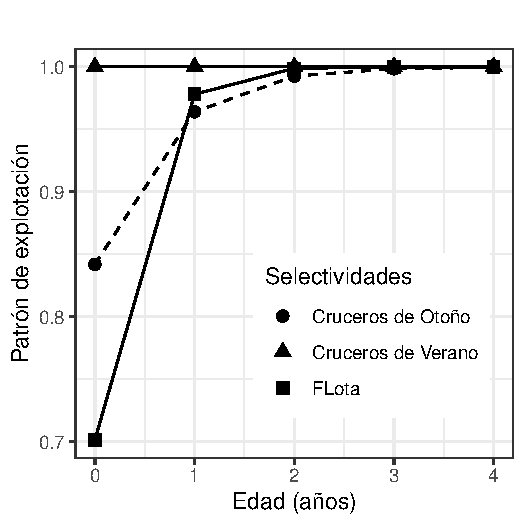
\includegraphics{FigurasInforme_Marzo/F36_selSept-1} \end{center}

\small

\textbf{Figura 36}. Patrón de explotación o selectividad de la flota y
de los cruceros acústicos de sardina común de las Regiones de Valparaíso
a Los Lagos. \vspace{0.5cm} \normalsize

\hypertarget{puntos-bioluxf3gicos-de-referencia-pbrs}{%
\subsubsection{4.2.2. Puntos Biológicos de Referencia
(PBRs)}\label{puntos-bioluxf3gicos-de-referencia-pbrs}}

En la \textbf{Tabla 21} se muestran los valores calculados en la
asesoría de septiembre 2020 y marzo 2021 de BD\textsubscript{0},
BD\textsubscript{RMS}, BD\textsubscript{LIM} y
F\textsubscript{RMS},recomendados por el Comité Científico Técnicos de
Pelágicos Pequeños (Informe Técnico CCT-PP N°01/2015) de acuerdo con la
metodología discutida durante el segundo taller (Abril, 2014) y tercer
taller (Agosto, 2014) de PBRs (Payá \emph{et al}. 2014). El valor
mediano de la mortalidad por pesca experimentado históricamente
(\(F_{mh}\)) por el stock de sardina común centro-sur cercano a
F53\%BDPR un porcentaje bajo considerando los altos niveles de
mortalidad por pesca que ha experimentado el stock (bajo el valor de
mortalidad natural, M=1,0 año\textsuperscript{-1}) (\textbf{Figura 37}).
Esto podría explicarse por la ubicación de la curva de selectividad
respecto a la madurez, donde la selectividad se encuentra a la izquierda
de la curva de madurez, producto de que la pesquería presenta una alta
selección de juveniles, de manera que la selectividad de la flota
comienza antes de la madurez (\textbf{Figura 38}). Esta condición
produciría valores de F60\% más moderados, que aumentaría si la
selectividad fuese igual a la madurez.

\small
\begin{center} 
\textbf{Tabla 21.}
\end{center}
\begin{center} 
\vspace{-0.2cm} Puntos Biológicos de Referencia de biomasa (miles t) estimada en la asesoría de septiembre 2020 y marzo 2021 para sardina común, calculados siguiendo los pasos descritos en la metodología de este informe.

\end{center}
\vspace{-0.2cm} 
\begin{table}[h]
    \centering
    \resizebox{13cm}{!} {
    \begin{tabular}{|c|l|l|c|c|}
    \hline
 Etapas & Cálculo                               & Aproximación       & Sept 2020   & Marzo 2021      \\ \hline
        & Promedio de la serie histórica entre  & $BD_{promedio}$    & 723 mil t   & 702 mil t. \\
 Paso 1 & 1991-2020 de la evaluación de stock   &                    &             &            \\
        & Mediana de la serie histórica entre   & $F_{mh}$           & 0.39        & 0.38       \\ 
        & 1991-2020 de la evaluación de stock   &                    &             &            \\ \hline                 
 Paso 2 & Cálculo de la curva de biomasa        & $\%BDPR (F_{mh})$  & 52.5\%      &  52.9\%    \\
        & por recluta (BDPR)                    & $\%BDPR (F_{RMS})$ & 60\%        &  60\%       \\ \hline
 Paso 3 & $\%BDPR (F_{mh}) - 5\%$               & $\%BD (F_{mh})$    & 47.5\%      &  47.9\%     \\
        & $\%BDPR (F_{RMS}) - 5\%$              & $\%BD (F_{RMS})$   & 55\%        &  55\%        \\ \hline
 Paso 4 & $BD_0=BD_{promedio} / \%BD_{Fmh}$     & $BD_0$             & 1.51 millón de t & 1.46 millón t. \\ \hline
 Paso 5 & $BD_{RMS} = BD_0*\%BD(F_{RMS})$       & $BD_{55\%}$        &  830 mil t  &  801 mil t. \\ \hline
 Paso 6 & $BD_{LIM} = BD_0 * \%BD(F_{LIM})$     & $BD_{27,5\%}$      &  415 mil t  &  401 mil t. \\ \hline
  \end{tabular}}
        \end{table}
\normalsize

\begin{center}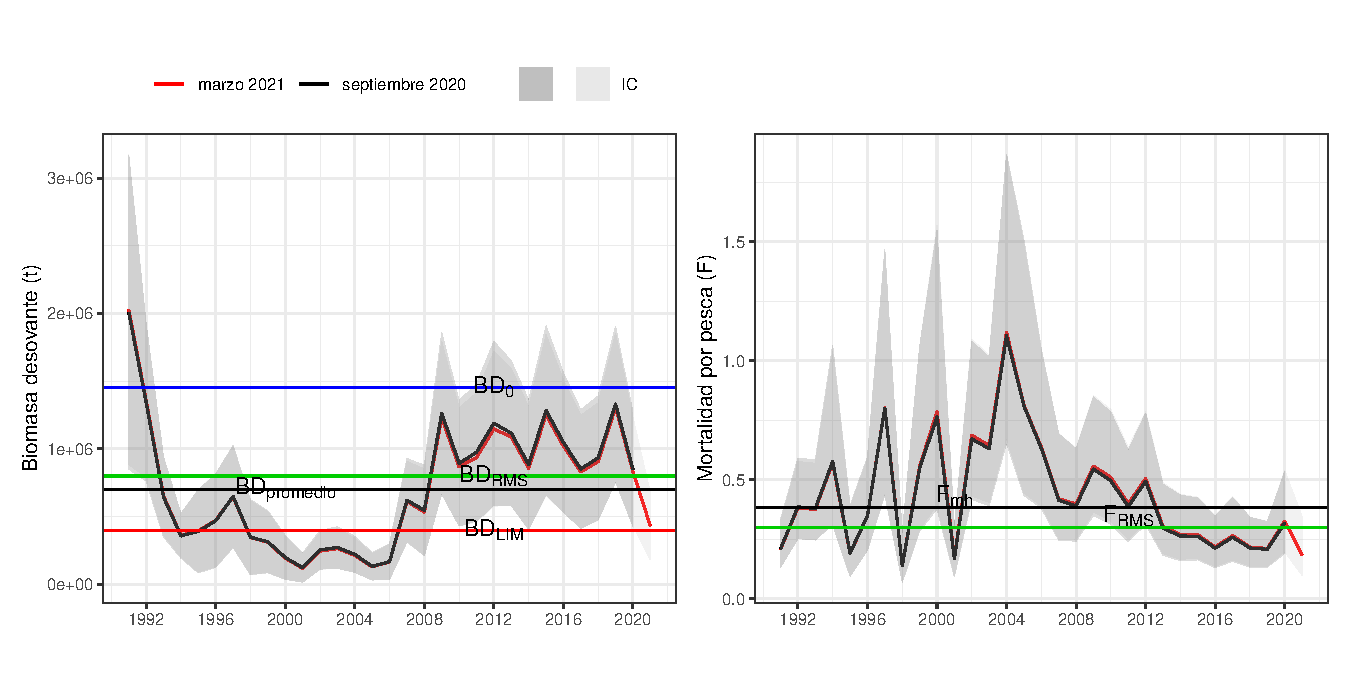
\includegraphics{FigurasInforme_Marzo/F37_PBRs_Bmed_Fmed-1} \end{center}

\vspace{-0.5cm}
\small

\textbf{Figura 37}. Series de Biomasa desovante y mortalidad por pesca
junto a los PBRs calculados a partir de la BD promedio y mediana de F
(Fmh). Los años en el eje x corresponden a año biológico. \normalsize

\begin{center}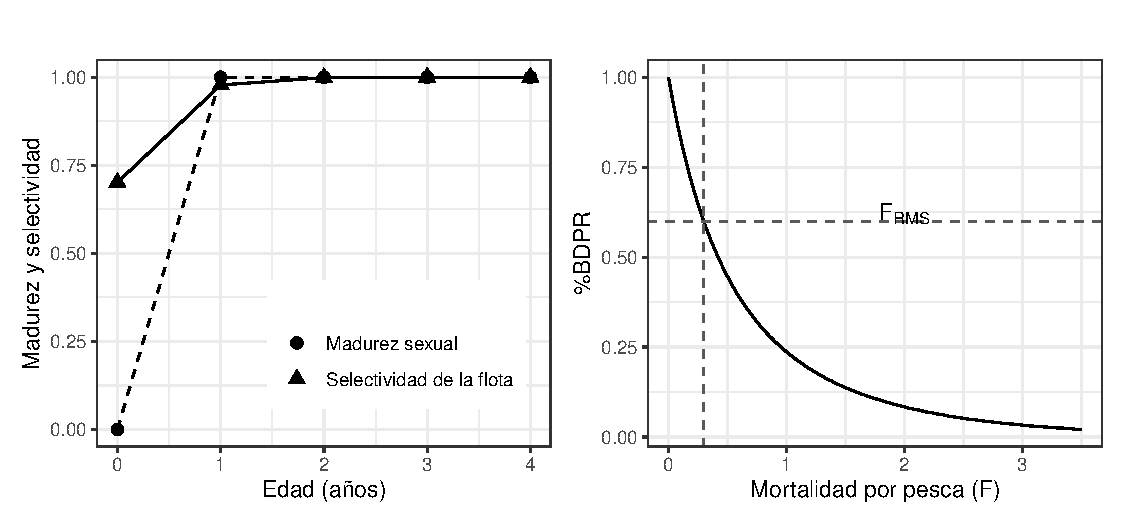
\includegraphics{FigurasInforme_Marzo/F38_madurezyselectividad-1} \end{center}

\small

\textbf{Figura 38}. Madurez, selectividad (Panel izquierdo) y Curva de
Biomasa por Recluta (\%BDPR) (Panel derecho), utilizados en los cálculos
de \(F_{RMS}\). \vspace{0.5cm} \normalsize

\hypertarget{estado-de-explotaciuxf3n}{%
\subsubsection{4.2.3. Estado de
explotación}\label{estado-de-explotaciuxf3n}}

La \textbf{Figura 39} muestra que en el inicio de la serie histórica la
biomasa indicaría una caída BD\textless BD\textsubscript{RMS} entre los
años 1994 y 1995 producto probablemente de fallas sucesivas en los
reclutamientos. El estado de la pesquería de sardina común durante los
años 1998 y 2006 estuvo marcado por condiciones ambientales ``El Niño''
1997-1998, provocando la caída hacia niveles inferiores de la biomasa
desovante límite (BD\textsubscript{LIM}) bajo el cual una pesquería
califica de agotada o colapsada. A partir del 2007 comienza un período
favorable para la condición de sardina común, ingresando a un proceso de
expansión poblacional que permite el año 2009 desplazarse hacia un nivel
de biomasa desovante superior al BD\textsubscript{RMS}. En la evaluación
actual (marzo 2021) la BD\textsubscript{2020/2021} esperada está un 46\%
bajo BD\textsubscript{RMS} (\textbf{Figura 39}). Dado que la biomasa
desovante se sustenta principalmente por la fracción adulta de
individuos (edad 1+), cuya abundancia disminuyó producto de bajos
reclutamientos ocurridos por dos años consecutivos (2019 - 2020), la
biomasa desovante del año biológico 2020/21 se redujo significativamente
respecto de años previos, posicionándola en una condición desfavorable
por debajo del objetivo de manejo.

En términos de la mortalidad por pesca (Ft año\textsuperscript{-1}),
ésta se había mantenido por sobre el nivel objetivo de referencia
F\textsubscript{RMS} en prácticamente toda la serie histórica analizada
producto de la alta selección de juveniles capturados antes de que estos
maduren (\textbf{Figura 39}). La alta selectividad de juveniles conlleva
a un valor de F\textsubscript{RMS} (F60\%BDPR) más moderado que una
selectividad cercana o por sobre la ojiva de madurez. A partir del año
2013 los niveles de Ft se han mantenido bajo el nivel de referencia
generado posiblemente por las caídas de los reclutamientos en algunos
años y las bajas CBAs recomendadas luego de la implementación de los
PBRs. Con respecto a la razón entre F\textsubscript{2020/21} y
F\textsubscript{RMS} fue de 0.61, siendo un 39\% menor a
F\textsubscript{RMS}, no obstante, este valor se debe considerar
preliminar ya que está basado en un supuesto de captura 2020/21
(\textbf{Figura 39}).

La condición estimada con información preliminar para el año 2020/2021
indica que la sardina común se encuentra en sobreexplotación (46\% bajo
BD\textsubscript{RMS} y 39\% bajo F\textsubscript{RMS}), con un 38\% de
probabilidad de colapso y sin riesgo de sobrepesca (\textbf{Tabla 24} y
\textbf{Figura 41}).

\begin{center}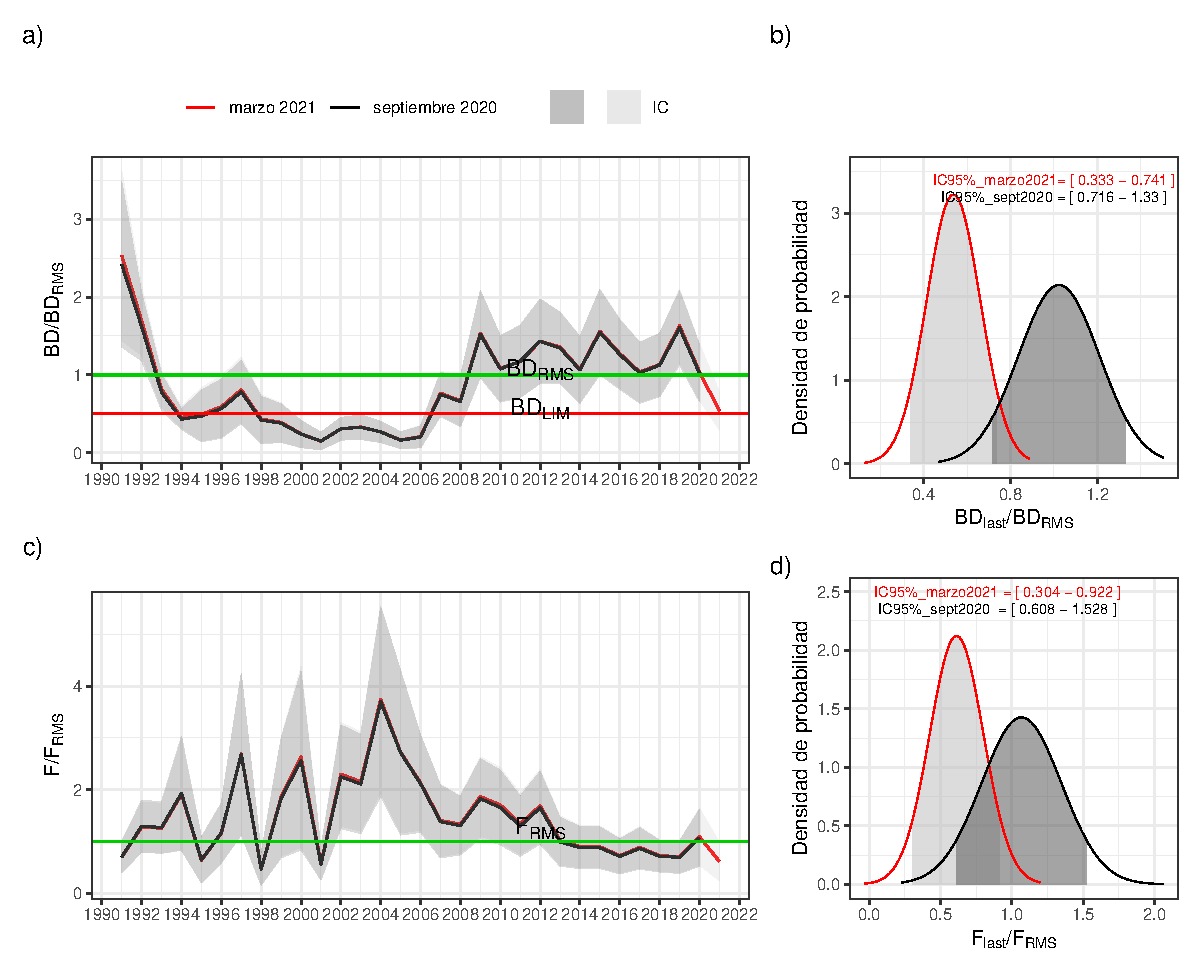
\includegraphics{FigurasInforme_Marzo/F39_indicadoresStock-1} \end{center}

\vspace{-0.3cm}
\small

\textbf{Figura 39}. a) Razón \(BD/BD_{RMS}\), b) la distribución de
probabilidad de \(BD_{last}/BD_{RMS}\), c) razón \(F/F_{RMS}\) y d) la
distribución de probabilidad \(F_{last}/F_{RMS}\). Los años en el eje x
corresponden a año biológico. \vspace{0.1cm} \normalsize

\pagebreak

\small
\begin{center} 
\textbf{Tabla 22.}
\end{center}
\begin{center} 
\vspace{-0.2cm} Comparación de los índices de reducción de F respecto de $F_{RMS}$ ($F/F_{RMS}$), BD respecto de $BD_{RMS}$ ($BD/BD_{RMS}$) estimados en la asesoría de septiembre 2020 y marzo 2021 de sardina común de las Regiones de Valparaíso a Los Lagos.
\end{center}
\vspace{-0.2cm}

\begin{longtable}[]{@{}ccccc@{}}
\toprule
\begin{minipage}[b]{0.08\columnwidth}\centering
Años\strut
\end{minipage} & \begin{minipage}[b]{0.18\columnwidth}\centering
\(F/F_{RMS_{sept}}\)\strut
\end{minipage} & \begin{minipage}[b]{0.19\columnwidth}\centering
\(F/F_{RMS_{marzo}}\)\strut
\end{minipage} & \begin{minipage}[b]{0.20\columnwidth}\centering
\(BD/BD_{RMS_{sept}}\)\strut
\end{minipage} & \begin{minipage}[b]{0.21\columnwidth}\centering
\(BD/BD_{RMS_{marzo}}\)\strut
\end{minipage}\tabularnewline
\midrule
\endhead
\begin{minipage}[t]{0.08\columnwidth}\centering
1990/91\strut
\end{minipage} & \begin{minipage}[t]{0.18\columnwidth}\centering
0.7\strut
\end{minipage} & \begin{minipage}[t]{0.19\columnwidth}\centering
0.693\strut
\end{minipage} & \begin{minipage}[t]{0.20\columnwidth}\centering
2.419\strut
\end{minipage} & \begin{minipage}[t]{0.21\columnwidth}\centering
2.534\strut
\end{minipage}\tabularnewline
\begin{minipage}[t]{0.08\columnwidth}\centering
1991/92\strut
\end{minipage} & \begin{minipage}[t]{0.18\columnwidth}\centering
1.293\strut
\end{minipage} & \begin{minipage}[t]{0.19\columnwidth}\centering
1.279\strut
\end{minipage} & \begin{minipage}[t]{0.20\columnwidth}\centering
1.619\strut
\end{minipage} & \begin{minipage}[t]{0.21\columnwidth}\centering
1.696\strut
\end{minipage}\tabularnewline
\begin{minipage}[t]{0.08\columnwidth}\centering
1992/93\strut
\end{minipage} & \begin{minipage}[t]{0.18\columnwidth}\centering
1.27\strut
\end{minipage} & \begin{minipage}[t]{0.19\columnwidth}\centering
1.256\strut
\end{minipage} & \begin{minipage}[t]{0.20\columnwidth}\centering
0.777\strut
\end{minipage} & \begin{minipage}[t]{0.21\columnwidth}\centering
0.815\strut
\end{minipage}\tabularnewline
\begin{minipage}[t]{0.08\columnwidth}\centering
1993/94\strut
\end{minipage} & \begin{minipage}[t]{0.18\columnwidth}\centering
1.931\strut
\end{minipage} & \begin{minipage}[t]{0.19\columnwidth}\centering
1.911\strut
\end{minipage} & \begin{minipage}[t]{0.20\columnwidth}\centering
0.431\strut
\end{minipage} & \begin{minipage}[t]{0.21\columnwidth}\centering
0.452\strut
\end{minipage}\tabularnewline
\begin{minipage}[t]{0.08\columnwidth}\centering
1994/95\strut
\end{minipage} & \begin{minipage}[t]{0.18\columnwidth}\centering
0.643\strut
\end{minipage} & \begin{minipage}[t]{0.19\columnwidth}\centering
0.637\strut
\end{minipage} & \begin{minipage}[t]{0.20\columnwidth}\centering
0.471\strut
\end{minipage} & \begin{minipage}[t]{0.21\columnwidth}\centering
0.493\strut
\end{minipage}\tabularnewline
\begin{minipage}[t]{0.08\columnwidth}\centering
1995/96\strut
\end{minipage} & \begin{minipage}[t]{0.18\columnwidth}\centering
1.164\strut
\end{minipage} & \begin{minipage}[t]{0.19\columnwidth}\centering
1.161\strut
\end{minipage} & \begin{minipage}[t]{0.20\columnwidth}\centering
0.566\strut
\end{minipage} & \begin{minipage}[t]{0.21\columnwidth}\centering
0.591\strut
\end{minipage}\tabularnewline
\begin{minipage}[t]{0.08\columnwidth}\centering
1996/97\strut
\end{minipage} & \begin{minipage}[t]{0.18\columnwidth}\centering
2.682\strut
\end{minipage} & \begin{minipage}[t]{0.19\columnwidth}\centering
2.689\strut
\end{minipage} & \begin{minipage}[t]{0.20\columnwidth}\centering
0.781\strut
\end{minipage} & \begin{minipage}[t]{0.21\columnwidth}\centering
0.808\strut
\end{minipage}\tabularnewline
\begin{minipage}[t]{0.08\columnwidth}\centering
1997/98\strut
\end{minipage} & \begin{minipage}[t]{0.18\columnwidth}\centering
0.461\strut
\end{minipage} & \begin{minipage}[t]{0.19\columnwidth}\centering
0.464\strut
\end{minipage} & \begin{minipage}[t]{0.20\columnwidth}\centering
0.42\strut
\end{minipage} & \begin{minipage}[t]{0.21\columnwidth}\centering
0.432\strut
\end{minipage}\tabularnewline
\begin{minipage}[t]{0.08\columnwidth}\centering
1998/99\strut
\end{minipage} & \begin{minipage}[t]{0.18\columnwidth}\centering
1.835\strut
\end{minipage} & \begin{minipage}[t]{0.19\columnwidth}\centering
1.859\strut
\end{minipage} & \begin{minipage}[t]{0.20\columnwidth}\centering
0.379\strut
\end{minipage} & \begin{minipage}[t]{0.21\columnwidth}\centering
0.389\strut
\end{minipage}\tabularnewline
\begin{minipage}[t]{0.08\columnwidth}\centering
1999/00\strut
\end{minipage} & \begin{minipage}[t]{0.18\columnwidth}\centering
2.561\strut
\end{minipage} & \begin{minipage}[t]{0.19\columnwidth}\centering
2.632\strut
\end{minipage} & \begin{minipage}[t]{0.20\columnwidth}\centering
0.239\strut
\end{minipage} & \begin{minipage}[t]{0.21\columnwidth}\centering
0.242\strut
\end{minipage}\tabularnewline
\begin{minipage}[t]{0.08\columnwidth}\centering
2000/01\strut
\end{minipage} & \begin{minipage}[t]{0.18\columnwidth}\centering
0.56\strut
\end{minipage} & \begin{minipage}[t]{0.19\columnwidth}\centering
0.576\strut
\end{minipage} & \begin{minipage}[t]{0.20\columnwidth}\centering
0.149\strut
\end{minipage} & \begin{minipage}[t]{0.21\columnwidth}\centering
0.148\strut
\end{minipage}\tabularnewline
\begin{minipage}[t]{0.08\columnwidth}\centering
2001/02\strut
\end{minipage} & \begin{minipage}[t]{0.18\columnwidth}\centering
2.249\strut
\end{minipage} & \begin{minipage}[t]{0.19\columnwidth}\centering
2.299\strut
\end{minipage} & \begin{minipage}[t]{0.20\columnwidth}\centering
0.307\strut
\end{minipage} & \begin{minipage}[t]{0.21\columnwidth}\centering
0.308\strut
\end{minipage}\tabularnewline
\begin{minipage}[t]{0.08\columnwidth}\centering
2002/03\strut
\end{minipage} & \begin{minipage}[t]{0.18\columnwidth}\centering
2.111\strut
\end{minipage} & \begin{minipage}[t]{0.19\columnwidth}\centering
2.155\strut
\end{minipage} & \begin{minipage}[t]{0.20\columnwidth}\centering
0.328\strut
\end{minipage} & \begin{minipage}[t]{0.21\columnwidth}\centering
0.33\strut
\end{minipage}\tabularnewline
\begin{minipage}[t]{0.08\columnwidth}\centering
2003/04\strut
\end{minipage} & \begin{minipage}[t]{0.18\columnwidth}\centering
3.701\strut
\end{minipage} & \begin{minipage}[t]{0.19\columnwidth}\centering
3.751\strut
\end{minipage} & \begin{minipage}[t]{0.20\columnwidth}\centering
0.267\strut
\end{minipage} & \begin{minipage}[t]{0.21\columnwidth}\centering
0.269\strut
\end{minipage}\tabularnewline
\begin{minipage}[t]{0.08\columnwidth}\centering
2004/05\strut
\end{minipage} & \begin{minipage}[t]{0.18\columnwidth}\centering
2.713\strut
\end{minipage} & \begin{minipage}[t]{0.19\columnwidth}\centering
2.724\strut
\end{minipage} & \begin{minipage}[t]{0.20\columnwidth}\centering
0.16\strut
\end{minipage} & \begin{minipage}[t]{0.21\columnwidth}\centering
0.163\strut
\end{minipage}\tabularnewline
\begin{minipage}[t]{0.08\columnwidth}\centering
2005/06\strut
\end{minipage} & \begin{minipage}[t]{0.18\columnwidth}\centering
2.116\strut
\end{minipage} & \begin{minipage}[t]{0.19\columnwidth}\centering
2.131\strut
\end{minipage} & \begin{minipage}[t]{0.20\columnwidth}\centering
0.202\strut
\end{minipage} & \begin{minipage}[t]{0.21\columnwidth}\centering
0.208\strut
\end{minipage}\tabularnewline
\begin{minipage}[t]{0.08\columnwidth}\centering
2006/07\strut
\end{minipage} & \begin{minipage}[t]{0.18\columnwidth}\centering
1.383\strut
\end{minipage} & \begin{minipage}[t]{0.19\columnwidth}\centering
1.405\strut
\end{minipage} & \begin{minipage}[t]{0.20\columnwidth}\centering
0.748\strut
\end{minipage} & \begin{minipage}[t]{0.21\columnwidth}\centering
0.765\strut
\end{minipage}\tabularnewline
\begin{minipage}[t]{0.08\columnwidth}\centering
2007/08\strut
\end{minipage} & \begin{minipage}[t]{0.18\columnwidth}\centering
1.305\strut
\end{minipage} & \begin{minipage}[t]{0.19\columnwidth}\centering
1.331\strut
\end{minipage} & \begin{minipage}[t]{0.20\columnwidth}\centering
0.658\strut
\end{minipage} & \begin{minipage}[t]{0.21\columnwidth}\centering
0.667\strut
\end{minipage}\tabularnewline
\begin{minipage}[t]{0.08\columnwidth}\centering
2008/09\strut
\end{minipage} & \begin{minipage}[t]{0.18\columnwidth}\centering
1.825\strut
\end{minipage} & \begin{minipage}[t]{0.19\columnwidth}\centering
1.865\strut
\end{minipage} & \begin{minipage}[t]{0.20\columnwidth}\centering
1.522\strut
\end{minipage} & \begin{minipage}[t]{0.21\columnwidth}\centering
1.536\strut
\end{minipage}\tabularnewline
\begin{minipage}[t]{0.08\columnwidth}\centering
2009/10\strut
\end{minipage} & \begin{minipage}[t]{0.18\columnwidth}\centering
1.657\strut
\end{minipage} & \begin{minipage}[t]{0.19\columnwidth}\centering
1.707\strut
\end{minipage} & \begin{minipage}[t]{0.20\columnwidth}\centering
1.077\strut
\end{minipage} & \begin{minipage}[t]{0.21\columnwidth}\centering
1.083\strut
\end{minipage}\tabularnewline
\begin{minipage}[t]{0.08\columnwidth}\centering
2010/11\strut
\end{minipage} & \begin{minipage}[t]{0.18\columnwidth}\centering
1.295\strut
\end{minipage} & \begin{minipage}[t]{0.19\columnwidth}\centering
1.335\strut
\end{minipage} & \begin{minipage}[t]{0.20\columnwidth}\centering
1.174\strut
\end{minipage} & \begin{minipage}[t]{0.21\columnwidth}\centering
1.17\strut
\end{minipage}\tabularnewline
\begin{minipage}[t]{0.08\columnwidth}\centering
2011/12\strut
\end{minipage} & \begin{minipage}[t]{0.18\columnwidth}\centering
1.651\strut
\end{minipage} & \begin{minipage}[t]{0.19\columnwidth}\centering
1.688\strut
\end{minipage} & \begin{minipage}[t]{0.20\columnwidth}\centering
1.433\strut
\end{minipage} & \begin{minipage}[t]{0.21\columnwidth}\centering
1.433\strut
\end{minipage}\tabularnewline
\begin{minipage}[t]{0.08\columnwidth}\centering
2012/13\strut
\end{minipage} & \begin{minipage}[t]{0.18\columnwidth}\centering
0.991\strut
\end{minipage} & \begin{minipage}[t]{0.19\columnwidth}\centering
1.016\strut
\end{minipage} & \begin{minipage}[t]{0.20\columnwidth}\centering
1.345\strut
\end{minipage} & \begin{minipage}[t]{0.21\columnwidth}\centering
1.358\strut
\end{minipage}\tabularnewline
\begin{minipage}[t]{0.08\columnwidth}\centering
2013/14\strut
\end{minipage} & \begin{minipage}[t]{0.18\columnwidth}\centering
0.881\strut
\end{minipage} & \begin{minipage}[t]{0.19\columnwidth}\centering
0.901\strut
\end{minipage} & \begin{minipage}[t]{0.20\columnwidth}\centering
1.065\strut
\end{minipage} & \begin{minipage}[t]{0.21\columnwidth}\centering
1.071\strut
\end{minipage}\tabularnewline
\begin{minipage}[t]{0.08\columnwidth}\centering
2014/15\strut
\end{minipage} & \begin{minipage}[t]{0.18\columnwidth}\centering
0.878\strut
\end{minipage} & \begin{minipage}[t]{0.19\columnwidth}\centering
0.898\strut
\end{minipage} & \begin{minipage}[t]{0.20\columnwidth}\centering
1.547\strut
\end{minipage} & \begin{minipage}[t]{0.21\columnwidth}\centering
1.561\strut
\end{minipage}\tabularnewline
\begin{minipage}[t]{0.08\columnwidth}\centering
2015/16\strut
\end{minipage} & \begin{minipage}[t]{0.18\columnwidth}\centering
0.71\strut
\end{minipage} & \begin{minipage}[t]{0.19\columnwidth}\centering
0.726\strut
\end{minipage} & \begin{minipage}[t]{0.20\columnwidth}\centering
1.262\strut
\end{minipage} & \begin{minipage}[t]{0.21\columnwidth}\centering
1.275\strut
\end{minipage}\tabularnewline
\begin{minipage}[t]{0.08\columnwidth}\centering
2016/17\strut
\end{minipage} & \begin{minipage}[t]{0.18\columnwidth}\centering
0.865\strut
\end{minipage} & \begin{minipage}[t]{0.19\columnwidth}\centering
0.886\strut
\end{minipage} & \begin{minipage}[t]{0.20\columnwidth}\centering
1.026\strut
\end{minipage} & \begin{minipage}[t]{0.21\columnwidth}\centering
1.038\strut
\end{minipage}\tabularnewline
\begin{minipage}[t]{0.08\columnwidth}\centering
2017/18\strut
\end{minipage} & \begin{minipage}[t]{0.18\columnwidth}\centering
0.713\strut
\end{minipage} & \begin{minipage}[t]{0.19\columnwidth}\centering
0.725\strut
\end{minipage} & \begin{minipage}[t]{0.20\columnwidth}\centering
1.126\strut
\end{minipage} & \begin{minipage}[t]{0.21\columnwidth}\centering
1.133\strut
\end{minipage}\tabularnewline
\begin{minipage}[t]{0.08\columnwidth}\centering
2018/19\strut
\end{minipage} & \begin{minipage}[t]{0.18\columnwidth}\centering
0.693\strut
\end{minipage} & \begin{minipage}[t]{0.19\columnwidth}\centering
0.705\strut
\end{minipage} & \begin{minipage}[t]{0.20\columnwidth}\centering
1.603\strut
\end{minipage} & \begin{minipage}[t]{0.21\columnwidth}\centering
1.632\strut
\end{minipage}\tabularnewline
\begin{minipage}[t]{0.08\columnwidth}\centering
2019/20\strut
\end{minipage} & \begin{minipage}[t]{0.18\columnwidth}\centering
1.068\strut
\end{minipage} & \begin{minipage}[t]{0.19\columnwidth}\centering
1.091\strut
\end{minipage} & \begin{minipage}[t]{0.20\columnwidth}\centering
1.023\strut
\end{minipage} & \begin{minipage}[t]{0.21\columnwidth}\centering
1.04\strut
\end{minipage}\tabularnewline
\begin{minipage}[t]{0.08\columnwidth}\centering
2020/21\strut
\end{minipage} & \begin{minipage}[t]{0.18\columnwidth}\centering
NA\strut
\end{minipage} & \begin{minipage}[t]{0.19\columnwidth}\centering
0.613\strut
\end{minipage} & \begin{minipage}[t]{0.20\columnwidth}\centering
NA\strut
\end{minipage} & \begin{minipage}[t]{0.21\columnwidth}\centering
0.537\strut
\end{minipage}\tabularnewline
\bottomrule
\end{longtable}

\pagebreak

\small
\begin{center} 
\textbf{Tabla 23.}
\end{center}
\begin{center} 
\vspace{-0.2cm} Comparación de las tasas de explotación anual referidos a la biomasa ($Y/BT$) y a la abundancia estimada ($C\#/N\#$), estimadas en la evaluación de septiembre 2020 y marzo 2021 de sardina común de las Regiones de Valparaíso a Los Lagos.
\end{center}
\vspace{-0.2cm}

\begin{longtable}[]{@{}ccccc@{}}
\toprule
Años & \(Y/BT_{sept}\) & \(Y/BT_{marzo}\) & \(C/N_{sept}\) &
\(C/N_{marzo}\)\tabularnewline
\midrule
\endhead
1990/91 & 0.174 & 0.172 & 0.102 & 0.101\tabularnewline
1991/92 & 0.264 & 0.261 & 0.179 & 0.178\tabularnewline
1992/93 & 0.262 & 0.26 & 0.169 & 0.167\tabularnewline
1993/94 & 0.398 & 0.395 & 0.232 & 0.23\tabularnewline
1994/95 & 0.158 & 0.157 & 0.088 & 0.088\tabularnewline
1995/96 & 0.238 & 0.238 & 0.148 & 0.149\tabularnewline
1996/97 & 0.512 & 0.513 & 0.323 & 0.324\tabularnewline
1997/98 & 0.099 & 0.1 & 0.069 & 0.069\tabularnewline
1998/99 & 0.326 & 0.33 & 0.233 & 0.236\tabularnewline
1999/00 & 0.432 & 0.442 & 0.291 & 0.298\tabularnewline
2000/01 & 0.115 & 0.118 & 0.074 & 0.076\tabularnewline
2001/02 & 0.438 & 0.445 & 0.261 & 0.266\tabularnewline
2002/03 & 0.383 & 0.39 & 0.252 & 0.256\tabularnewline
2003/04 & 0.501 & 0.505 & 0.39 & 0.394\tabularnewline
2004/05 & 0.401 & 0.403 & 0.302 & 0.304\tabularnewline
2005/06 & 0.394 & 0.397 & 0.237 & 0.239\tabularnewline
2006/07 & 0.334 & 0.339 & 0.193 & 0.196\tabularnewline
2007/08 & 0.24 & 0.245 & 0.158 & 0.161\tabularnewline
2008/09 & 0.331 & 0.337 & 0.229 & 0.234\tabularnewline
2009/10 & 0.334 & 0.343 & 0.209 & 0.215\tabularnewline
2010/11 & 0.276 & 0.283 & 0.164 & 0.169\tabularnewline
2011/12 & 0.313 & 0.319 & 0.202 & 0.206\tabularnewline
2012/13 & 0.224 & 0.229 & 0.147 & 0.15\tabularnewline
2013/14 & 0.165 & 0.168 & 0.116 & 0.119\tabularnewline
2014/15 & 0.185 & 0.189 & 0.119 & 0.122\tabularnewline
2015/16 & 0.157 & 0.16 & 0.104 & 0.107\tabularnewline
2016/17 & 0.149 & 0.153 & 0.114 & 0.117\tabularnewline
2017/18 & 0.127 & 0.129 & 0.097 & 0.098\tabularnewline
2018/19 & 0.174 & 0.176 & 0.105 & 0.107\tabularnewline
2019/20 & 0.217 & 0.222 & 0.152 & 0.155\tabularnewline
2020/21 & NA & 0.123 & NA & 0.08\tabularnewline
\bottomrule
\end{longtable}

\normalsize

\pagebreak

\begin{center}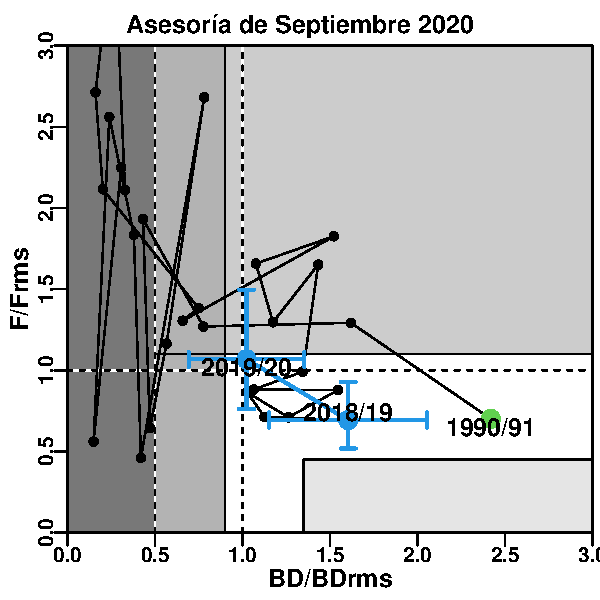
\includegraphics{FigurasInforme_Marzo/Fig40_DFsept-1} \end{center}

\vspace{-0.3cm}
\footnotesize

\begin{center}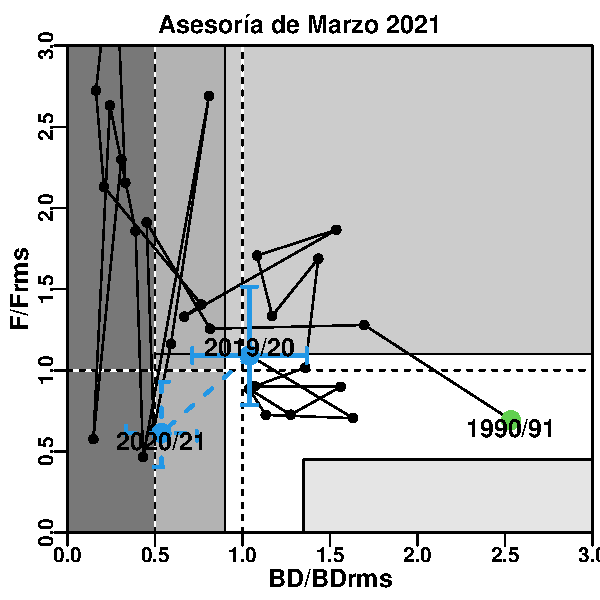
\includegraphics{FigurasInforme_Marzo/Fig41_DFmarzo-1} \end{center}

\vspace{-0.3cm}
\footnotesize

\textbf{Figura 41}. Diagrama de fases de explotación de la biomasa
desovante respecto de la mortalidad por pesca de la asesoría de
septiembre 2020 (panel superior) y marzo 2021 (panel inferior). Los ejes
están estandarizados a los valores que generan el RMS proxy. Cruz azul
corresponde a los intervalos de confianza de la razón
BD/BD\textsubscript{RMS} y F/F\textsubscript{RMS}. El año con cruz
continua corresponde a ``\emph{Estatus completo}'' y la cruz con línea
discontinua a ``\emph{Estatus preliminar}''. \vspace{0.5cm} \normalsize

\pagebreak

\small
\begin{center} 
\textbf{Tabla 24.}
\end{center}
\begin{center} 
\vspace{-0.2cm} Puntos Biológicos de referencia (PBRs) y probabilidades de estar bajo $BD_{RMS}$ y sobre $F_{RMS}$ y en sobreexplotación, colapsado o sobrepesca. 
\end{center}
\vspace{-0.2cm}

\begin{longtable}[]{@{}lcc@{}}
\toprule
& Septiembre 2020 & Marzo 2021\tabularnewline
\midrule
\endhead
Año biológico & 2019/20 & 2020/21\tabularnewline
\(F_{RMS}\) & 0.3 & 0.3\tabularnewline
\(BD_{RMS}\) & 830 & 801\tabularnewline
\(BD_{LIM}\) & 415 & 401\tabularnewline
\(p(BD_{last}<BD_{RMS})\) & 0.45 & 1\tabularnewline
\(p(F_{last}>F_{RMS})\) & 0.6 & 0.02\tabularnewline
\(p(sobre-explotación)\) & 0.26 & 1\tabularnewline
\(p(agotado/colapsado)\) & 0 & 0.38\tabularnewline
\(p(sobrepesca)\) & 0.45 & 0\tabularnewline
\bottomrule
\end{longtable}

\vspace{-0.5cm}
\scriptsize

\begin{itemize}
\tightlist
\item
  \(p(BD_{last}<BD_{RMS})\) = Probabilidad de que BD del año más
  reciente sea menor a \(BD_{RMS}\)
\item
  \(p(F_{last}>F_{RMS})\) = Probabilidad que la Ft del año más reciente
  sea menor a \(F_{RMS}\)
\item
  Probabilidad de estar en sobreexplotación =
  \(p(BD_{last}<0,9BD_{RMS})\)
\item
  Probabilidad de estar en colapso = \(p(BD_{last}<BD_{LIM})\)
\item
  Probabilidad de estar en sobrepesca = \(p(F_{last}>1,1F_{RMS})\)
\end{itemize}

\normalsize

\pagebreak

\hypertarget{objetivo-especuxedfico-3-1}{%
\subsection{4.3. Objetivo específico
3:}\label{objetivo-especuxedfico-3-1}}

\vspace{-0.2cm}

\emph{``Determinar niveles de Captura Biológicamente Aceptable (CBA) que
lleven y/o mantenga la pesquería en torno al Rendimiento Máximo
Sostenible (RMS), a partir de un análisis de riesgo en condiciones de
incertidumbre de no alcanzar los objetivos de conservación y
sostenibilidad conforme lo establece la LGPA y contenidos en el Plan de
Manejo y/o en el Programa de Recuperación respectivo, según
corresponda.''}

\hypertarget{cba-2021-inicial-asesoruxeda-de-septiembre-2020}{%
\subsubsection{CBA 2021 Inicial (Asesoría de septiembre
2020)}\label{cba-2021-inicial-asesoruxeda-de-septiembre-2020}}

Para el cálculo CBA 2021 se proyectó la población 2 años biológicos
hacia el futuro (julio2020-junio2021 y julio2021-junio2022) en base a
tres escenarios de reclutamiento: a) un escenario desfavorable que
consiste en el reclutamiento promedio del período 1991-2007 (113 mil
millones de ind.), b) un escenario favorable que corresponde al promedio
de los reclutamientos del período 2008 - 2012 (411 mil millones de ind.)
y un escenario que representa el período reciente entre el 2013-2020
(173 mil millones de ind.) (\textbf{Figura 42}). \vspace{0.5cm}

\begin{center}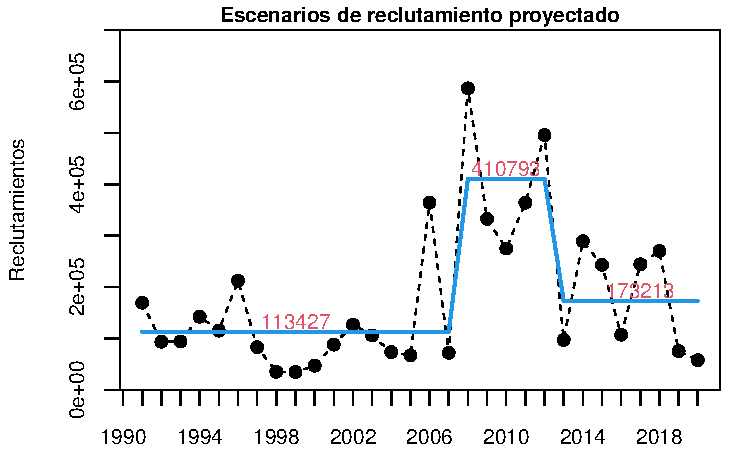
\includegraphics{FigurasInforme_Marzo/Fig42_Reclproy_sept-1} \end{center}

\small

\textbf{Figura 42}. Escenarios de reclutamiento proyectado asesoría de
septiembre 2020. \vspace{0.5cm} \normalsize

El cálculo de la CBA inicial para el año calendario 2021 se obtiene como
el promedio ponderado según la estacionalidad semestral de la pesquería
que a la fecha se asume 70\% para el primer semestre y 30\% para el
segundo semestre, bajo un criterio de explotación de F60\%SPR, sujeto a
percentiles de probabilidad entre el 10\% y 50\%.

La \textbf{Tabla 25} muestra los rangos de capturas para el año 2021
estimada bajo un escenario de Rprom(1991-2007) podría situarse entre 195
mil t. y 250 mil t. y bajo un escenario de Rprom(2008-2012) entre 353
mil t. y 448 mil t. y bajo un escenario de Rprom(2013-2020) entre 223
mil t. y 301 mil t.

Para evaluar el efecto que tiene la decisión de la CBA en base a los
percentiles (10\%-50\%) que en general son menores a la captura al RMS
(percentil del 50\%), se calculó el resguardo a lo cual equivale cada
percentil (\textbf{Tabla 26}). Esos niveles variaron entre un 5\% para
un percentil del 40\% a un 22\% en promedio, considerando un percentil
de probabilidad del 10\% para los tres escenarios de reclutamiento.

Considerando que no se cuenta con el \% de descarte actualizado al 2020,
para la asesoría de septiembre 2020 se muestran 2 escenarios de
descarte, la \textbf{Tabla 27} muestra los rangos de captura menos el
2\% correspondiente al descarte 2017 y la \textbf{Tabla 28} muestra los
rangos de captura con el descuento del 6\% (descarte 2019).

En la secta sesión del CCT-PP 2020 (Acta de Sesión Nº6, octubre 2020
\footnote{\url{https://www.subpesca.cl/portal/616/articles-108975_documento.pdf}}.)
se recomendó una CBA máxima 2021 de 201.409 toneladas correspondiente al
escenario de reclutamiento promedio bajo (1991-2007), 20\% de percentil
de captura (equivalente a un 14\% resguardo) y el descuento del 6\% de
descarte (\textbf{Tabla 28}).

\vspace{0.5cm}

\small
\begin{center} 
\textbf{Tabla 25.}
\end{center}
\begin{center} 
\vspace{-0.2cm} CBA inicial 2021 de sardina común calculada bajo $F_{RMS}$ , con sus respectivos percentiles de captura entre 10\% y 50\% y tres escenarios de reclutamientos.
\end{center}
\vspace{-0.2cm}

\begin{longtable}[]{@{}lrrr@{}}
\toprule
& 1991-2007 & 2008-2012 & 2013-2020\tabularnewline
\midrule
\endhead
mean & 250260 & 447840 & 300810\tabularnewline
std & 42769 & 73667 & 60397\tabularnewline
10\% & 195449 & 353432 & 223408\tabularnewline
20\% & 214265 & 385840 & 249979\tabularnewline
30\% & 227832 & 409209 & 269138\tabularnewline
40\% & 239425 & 429177 & 285509\tabularnewline
50\% & 250260 & 447840 & 300810\tabularnewline
\bottomrule
\end{longtable}

\vspace{-0.5cm}

\small
\begin{center} 
\textbf{Tabla 26.}
\end{center}
\begin{center} 
\vspace{-0.2cm} Reguardo de la Captura al RMS.
\end{center}
\vspace{-0.2cm}

\begin{longtable}[]{@{}lrrr@{}}
\toprule
& 1991-2007 & 2008-2012 & 2013-2020\tabularnewline
\midrule
\endhead
10\% & 0.22 & 0.21 & 0.26\tabularnewline
20\% & 0.14 & 0.14 & 0.17\tabularnewline
30\% & 0.09 & 0.09 & 0.11\tabularnewline
40\% & 0.04 & 0.04 & 0.05\tabularnewline
50\% & 0.00 & 0.00 & 0.00\tabularnewline
\bottomrule
\end{longtable}

\vspace{-0.5cm}

\small
\begin{center} 
\textbf{Tabla 27.}
\end{center}
\begin{center} 
\vspace{-0.2cm} CBA inicial 2021 menos el 2\%descarte. 
\end{center}
\vspace{-0.2cm}

\begin{longtable}[]{@{}lrrr@{}}
\toprule
& 1991-2007 & 2008-2012 & 2013-2020\tabularnewline
\midrule
\endhead
10\% & 191540 & 346363 & 218940\tabularnewline
20\% & 209979 & 378123 & 244979\tabularnewline
30\% & 223275 & 401025 & 263755\tabularnewline
40\% & 234636 & 420593 & 279798\tabularnewline
50\% & 245255 & 438883 & 294794\tabularnewline
\bottomrule
\end{longtable}

\vspace{-0.5cm}

\small
\begin{center} 
\textbf{Tabla 28.}
\end{center}
\begin{center} 
\vspace{-0.2cm} CBA inicial 2021 menos el 6\%descarte.*CBA máxima recomendada por el CCT-PP = 201.409 t.
\end{center}
\vspace{-0.2cm}

\begin{longtable}[]{@{}lrrr@{}}
\toprule
& 1991-2007 & 2008-2012 & 2013-2020\tabularnewline
\midrule
\endhead
10\% & 183722 & 332226 & 210004\tabularnewline
20\% & 201409 & 362690 & 234980\tabularnewline
30\% & 214162 & 384656 & 252990\tabularnewline
40\% & 225059 & 403426 & 268378\tabularnewline
50\% & 235244 & 420970 & 282761\tabularnewline
\bottomrule
\end{longtable}

\normalsize

\pagebreak

\hypertarget{primera-revisiuxf3n-cba-2021-asesoruxeda-de-marzo-2021}{%
\subsubsection{Primera revisión CBA 2021 (Asesoría de marzo
2021)}\label{primera-revisiuxf3n-cba-2021-asesoruxeda-de-marzo-2021}}

Para el cálculo CBA 2021 se proyectó la población 1 año biológico hacia
el futuro (julio2021-junio2022) en base a tres escenarios de
reclutamiento: a) un escenario desfavorable que consiste en el
reclutamiento promedio del período 1991-2007 (113 mil millones de ind.),
b) un escenario favorable que corresponde al promedio de los
reclutamientos del período 2008 - 2012 (405 mil millones de ind.) y un
escenario que representa el período reciente entre el 2013-2021 (180 mil
millones de ind.) (\textbf{Figura 43}).

\vspace{0.5cm}

\begin{center}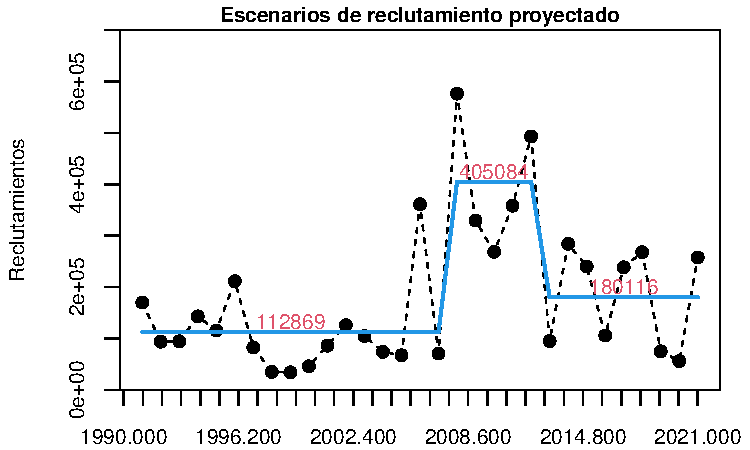
\includegraphics{FigurasInforme_Marzo/Fig43_Reclproy_marzo-1} \end{center}

\small

\textbf{Figura 43}. Escenarios de reclutamiento proyectado asesoría de
marzo 2021. \vspace{0.5cm} \normalsize

El cálculo de la primera revisión de la CBA para el año calendario 2021
se obtiene como el promedio ponderado según la estacionalidad semestral
de la pesquería que a la fecha se asume 70\% para el primer semestre y
30\% para el segundo semestre, bajo un criterio de explotación de
F60\%SPR, sujeto a percentiles de probabilidad de captura entre el 10\%
y 50\%.

La \textbf{Tabla 29} muestra los rangos de capturas para el año 2021
estimada bajo un escenario de Rprom(1990-2007) podría situarse entre 234
mil t. y 272 mil t. y bajo un escenario de Rprom(2008-2012) entre 269
mil t. y 313 mil t. y bajo un escenario de Rprom(2013-2021) entre 236
mil t. y 279 mil t.

Para evaluar el efecto que tiene la decisión de la CBA en base a los
percentiles (10\%-50\%) que en general son menores a la captura al RMS
(percentil del 50\%), se calculó el resguardo a lo cual equivale cada
percentil (\textbf{Tabla 30}). Esos niveles variaron entre un 3\% para
un percentil del 40\% a un 14\% en promedio, considerando un percentil
de probabilidad del 10\% para los tres escenarios de reclutamiento.

En la primera sesión del CCT-PP 2021 (febrero 2021) se acordó utilizar
un 4\% de descarte para el supuesto de descarte proyectado de sardina
común, en base a esto, la \textbf{Tabla 31} muestra los rangos de
captura menos el 4\% de descarte. La \textbf{Tabla 31b} muestra las
diferencias porcentuales entre la CBA inicial menos el 6\% de descarte y
la primera revisión de CBA 2012 menos el 4\%.

\vspace{0.5cm}

\pagebreak

\small
\begin{center} 
\textbf{Tabla 29.}
\end{center}
\begin{center} 
\vspace{-0.2cm} Primera revisión de CBA 2021 de sardina común calculada bajo $F_{RMS}$ , con sus respectivos percentiles de captura entre 10\% y 50\% y tres escenarios de reclutamientos.
\end{center}
\vspace{-0.2cm}

\begin{longtable}[]{@{}lrrr@{}}
\toprule
& 1991-2007 & 2008-2012 & 2013-2021\tabularnewline
\midrule
\endhead
mean & 271720 & 313030 & 279570\tabularnewline
std & 29384 & 34291 & 33911\tabularnewline
10\% & 234063 & 269084 & 236111\tabularnewline
20\% & 246990 & 284170 & 251030\tabularnewline
30\% & 256311 & 295048 & 261787\tabularnewline
40\% & 264276 & 304342 & 270979\tabularnewline
50\% & 271720 & 313030 & 279570\tabularnewline
\bottomrule
\end{longtable}

\vspace{-0.5cm}

\small
\begin{center} 
\textbf{Tabla 30.}
\end{center}
\begin{center} 
\vspace{-0.2cm} Reguardo de la Captura al RMS.
\end{center}
\vspace{-0.2cm}

\begin{longtable}[]{@{}lrrr@{}}
\toprule
& 1991-2007 & 2008-2012 & 2013-2021\tabularnewline
\midrule
\endhead
10\% & 0.14 & 0.14 & 0.16\tabularnewline
20\% & 0.09 & 0.09 & 0.10\tabularnewline
30\% & 0.06 & 0.06 & 0.06\tabularnewline
40\% & 0.03 & 0.03 & 0.03\tabularnewline
50\% & 0.00 & 0.00 & 0.00\tabularnewline
\bottomrule
\end{longtable}

\vspace{-0.5cm}

\small
\begin{center} 
\textbf{Tabla 31.}
\end{center}
\begin{center} 
\vspace{-0.2cm} CBA 2021 menos el 4\%descarte. 
\end{center}
\vspace{-0.2cm}

\begin{longtable}[]{@{}lrrr@{}}
\toprule
& 1991-2007 & 2008-2012 & 2013-2021\tabularnewline
\midrule
\endhead
10\% & 224700 & 258321 & 226667\tabularnewline
20\% & 237110 & 272803 & 240989\tabularnewline
30\% & 246059 & 283246 & 251316\tabularnewline
40\% & 253705 & 292169 & 260140\tabularnewline
50\% & 260851 & 300509 & 268387\tabularnewline
\bottomrule
\end{longtable}

\vspace{-0.5cm}

\small
\begin{center} 
\textbf{Tabla 31b.}
\end{center}
\begin{center} 
\vspace{-0.2cm} Diferencia porcentuales entre la CBA inicial menos el 6\%descarte y la primera revisión de CBA 2021 menos el 4\%descarte. (1-(1erarevisiónCBA/CBAinicial)*100)
\end{center}
\vspace{-0.2cm}

\begin{longtable}[]{@{}lrrr@{}}
\toprule
& 1991-2007 & 2008-2012 & 2013-2021\tabularnewline
\midrule
\endhead
10\% & 22 & -22 & 8\tabularnewline
20\% & 18 & -25 & 3\tabularnewline
30\% & 15 & -26 & -1\tabularnewline
40\% & 13 & -28 & -3\tabularnewline
50\% & 11 & -29 & -5\tabularnewline
\bottomrule
\end{longtable}

\normalsize

\pagebreak

\hypertarget{proyecciuxf3n-del-stock-asesoruxeda-de-septiembre-2020}{%
\subsubsection{4.3.2. Proyección del stock (Asesoría de septiembre
2020)}\label{proyecciuxf3n-del-stock-asesoruxeda-de-septiembre-2020}}

En relación al estatus 2020/21, se proyectó el stock bajo tres
escenarios reclutamientos 2021 que representan los períodos más
relevantes de la historia conocida de sardina común y con una mortalidad
por pesca en torno al F\textsubscript{RMS} (ponderadores de
F\textsubscript{RMS}). Al respecto, si bien la sardina se ha mantenido
en una condición de plena-explotación a partir del 2013 a la fecha, la
disminución del reclutamiento los años 2019 y 2020 junto a la
disminución de la biomasa adulta (1+ años) el 2020 generan una alta
probabilidad (100 \%) de sobreexplotación y un 42 \% de probabilidad de
colapso de sardina común para el año 2020/21 (\textbf{Tabla 32})
independiente de los escenario de reclutamiento futuros y ponderadores
de F\textsubscript{RMS} (\textbf{Figura 44}). En base a esta proyección,
era recomendable considerar un escenario de reclutamiento precautorio en
torno al promedio del período de reclutamientos bajos (1991-2007) para
la determinación de una captura 2021 biológicamente sustentable para
sardina común a la espera de la actualización de marzo y julio 2021.

\vspace{0.5cm}

\small
\begin{center} 
\textbf{Tabla 32.}
\end{center}
\begin{center} 
\vspace{-0.2cm} Incertidumbre del estatus previo 2018/19, actual 2019/20 y proyectado 2020/21 bajo tres escenarios de reclutamiento y ponderadores de $F_{RMS}$. Asesoría de septiembre 2020.
\end{center}
\vspace{-0.2cm}

\begin{longtable}[]{@{}lccc@{}}
\toprule
& 1991-2007{[}F\textsubscript{RMS}*1{]} & {[}F\textsubscript{RMS}*0.9{]}
& {[}F\textsubscript{RMS}*0.7{]}\tabularnewline
\midrule
\endhead
p(sobre-explotación)\_2018/19 & 0.00 & 0.00 & 0.00\tabularnewline
p(colapso)\_2018/19 & 0.00 & 0.00 & 0.00\tabularnewline
p(sobre-explotación)\_2019/20 & 0.26 & 0.26 & 0.26\tabularnewline
p(colapso)\_2019/20 & 0.00 & 0.00 & 0.00\tabularnewline
p(sobre-explotación)\_2020/21 & 1.00 & 1.00 & 1.00\tabularnewline
p(colapso)\_2020/21 & 0.42 & 0.41 & 0.40\tabularnewline
\bottomrule
\end{longtable}

\vspace{-0.7cm}

\begin{longtable}[]{@{}lccc@{}}
\toprule
& 2008-2012{[}F\textsubscript{RMS}*1{]} & {[}F\textsubscript{RMS}*0.9{]}
& {[}F\textsubscript{RMS}*0.7{]}\tabularnewline
\midrule
\endhead
p(sobre-explotación)\_2018/19 & 0.00 & 0.00 & 0.00\tabularnewline
p(colapso)\_2018/19 & 0.00 & 0.00 & 0.00\tabularnewline
p(sobre-explotación)\_2019/20 & 0.26 & 0.26 & 0.26\tabularnewline
p(colapso)\_2019/20 & 0.00 & 0.00 & 0.00\tabularnewline
p(sobre-explotación)\_2020/21 & 1.00 & 1.00 & 1.00\tabularnewline
p(colapso)\_2020/21 & 0.42 & 0.41 & 0.40\tabularnewline
\bottomrule
\end{longtable}

\vspace{-0.7cm}

\begin{longtable}[]{@{}lccc@{}}
\toprule
& 2013-2020{[}F\textsubscript{RMS}*1{]} & {[}F\textsubscript{RMS}*0.9{]}
& {[}F\textsubscript{RMS}*0.7{]}\tabularnewline
\midrule
\endhead
p(sobre-explotación)\_2018/19 & 0.00 & 0.00 & 0.00\tabularnewline
p(colapso)\_2018/19 & 0.00 & 0.00 & 0.00\tabularnewline
p(sobre-explotación)\_2019/20 & 0.26 & 0.26 & 0.26\tabularnewline
p(colapso)\_2019/20 & 0.00 & 0.00 & 0.00\tabularnewline
p(sobre-explotación)\_2020/21 & 1.00 & 1.00 & 1.00\tabularnewline
p(colapso)\_2020/21 & 0.42 & 0.41 & 0.40\tabularnewline
\bottomrule
\end{longtable}

\vspace{-0.7cm}
\scriptsize

\begin{itemize}
\tightlist
\item
  p{[}BD\textless0,9BD\textsubscript{RMS}{]} = probabilidad de
  sobre-explotación
\item
  p{[}BD\textless0,5BD\textsubscript{RMS}{]} = probabilidad de colapso
\end{itemize}

\pagebreak

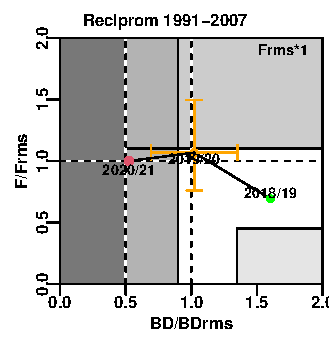
\includegraphics{FigurasInforme_Marzo/Fig44a_sept-1.pdf}
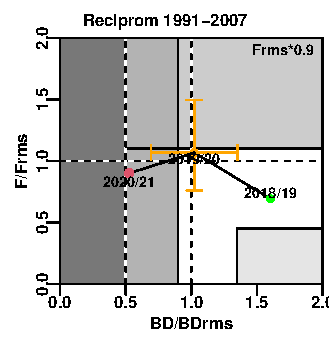
\includegraphics{FigurasInforme_Marzo/Fig44a_sept-2.pdf}
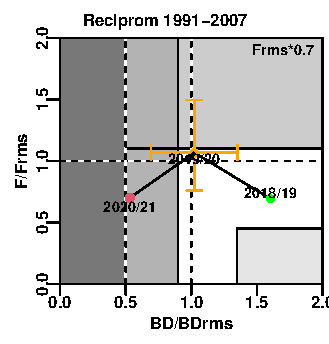
\includegraphics{FigurasInforme_Marzo/Fig44a_sept-3.pdf}

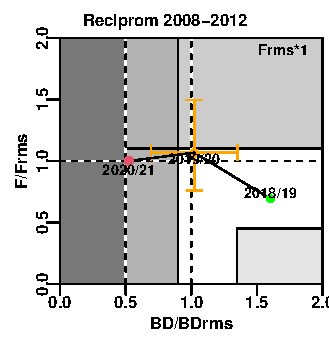
\includegraphics{FigurasInforme_Marzo/Fig44b_sept-1.pdf}
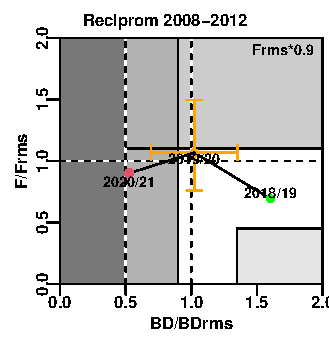
\includegraphics{FigurasInforme_Marzo/Fig44b_sept-2.pdf}
\includegraphics{FigurasInforme_Marzo/Fig44b_sept-3.pdf}

\includegraphics{FigurasInforme_Marzo/Fig44c_sept-1.pdf}
\includegraphics{FigurasInforme_Marzo/Fig44c_sept-2.pdf}
\includegraphics{FigurasInforme_Marzo/Fig44c_sept-3.pdf}

\small

\textbf{Figura 44}. Diagramas de fases de explotación de la biomasa
desovante respecto de la mortalidad por pesca mostrando el estatus de
sardina común para el año previo 2018/19 (punto verde), año actual
2019/20 (punto y cruz naranjo) y año proyectado 2020/21 (punto rojo)
bajo un escenario de reclutamiento promedio bajo {[}1991-2007{]} (panel
superior), reclutamiento promedio alto {[}2008-2012{]} (panel
intermedio), reclutamiento promedio reciente {[}2013-2020{]} (panel
inferior) y ponderadores de F\textsubscript{RMS} (1,0.9 y 0.7).
\textbf{Asesoría de septiembre 2020}. \vspace{0.5cm} \normalsize

\pagebreak

\hypertarget{proyecciuxf3n-del-stock-asesoruxeda-de-marzo-2021}{%
\subsubsection{4.3.3. Proyección del stock (Asesoría de marzo
2021)}\label{proyecciuxf3n-del-stock-asesoruxeda-de-marzo-2021}}

En relación al estatus 2020/21, en la asesoría previa (septiembre 2020)
la proyección mostraba una alta probabilidad (100 \%) de
sobreexplotación y un 42 \% de probabilidad de colapso de sardina común
para el año 2020/21 producto de la disminución del reclutamiento los
años 2019 y 2020 junto a la disminución de la biomasa adulta (1+ años)
el 2020 independiente de los escenario de reclutamiento futuros y
ponderadores de F\textsubscript{RMS} (\textbf{Tabla 32 y Figuras 44}).
La primera actualización del estatus 2020/21 con información del crucero
de venaro 2021 (asesoría de marzo 2021) confirman una condición de
sobreexplotación (100\% de probabilidad) y un 38\% de probabilidad de
colapso (\textbf{Tabla 33}).

No obstante, dado los altos niveles de reclutamiento estimados para el
2021 en base a la actualización de la información de biomasa total y
composición de edad del crucero de verano 2021 se proyecta una
recuperación del estatus para el año biológico 2021/22, retornando a una
condición de plena-explotación con un 26\% de probabilidad de
sobre-explotación y un 3\% de probabilidad de colapso (\textbf{Tabla 33
y Figura 45}), independiente del escenario de reclutamiento proyectado.

\vspace{0.5cm}

\small
\begin{center} 
\textbf{Tabla 33.}
\end{center}
\begin{center} 
\vspace{-0.2cm} Incertidumbre del estatus actual 2020/21 y proyectado 2021/22 bajo tres escenarios de reclutamiento y ponderadores de $F_{RMS}$
\end{center}
\vspace{-0.2cm}

\begin{longtable}[]{@{}lccc@{}}
\toprule
& 1991-2007{[}F\textsubscript{RMS}*1{]} & {[}F\textsubscript{RMS}*0.9{]}
& {[}F\textsubscript{RMS}*0.7{]}\tabularnewline
\midrule
\endhead
p(BD\textless0,9BD\textsubscript{RMS})\_2020/21 & 1.00 & 1.00 &
1.00\tabularnewline
p(BD\textless0,5BD\textsubscript{RMS})\_2020/21 & 0.38 & 0.38 &
0.38\tabularnewline
p(BD\textless0,9BD\textsubscript{RMS})\_2021/22 & 0.27 & 0.26 &
0.26\tabularnewline
p(BD\textless0,5BD\textsubscript{RMS})\_2021/22 & 0.04 & 0.03 &
0.03\tabularnewline
\bottomrule
\end{longtable}

\vspace{-0.7cm}

\begin{longtable}[]{@{}lccc@{}}
\toprule
& 2008-2012{[}F\textsubscript{RMS}*1{]} & {[}F\textsubscript{RMS}*0.9{]}
& {[}F\textsubscript{RMS}*0.7{]}\tabularnewline
\midrule
\endhead
p(BD\textless0,9BD\textsubscript{RMS})\_2020/21 & 1.00 & 1.00 &
1.00\tabularnewline
p(BD\textless0,5BD\textsubscript{RMS})\_2020/21 & 0.38 & 0.38 &
0.38\tabularnewline
p(BD\textless0,9BD\textsubscript{RMS})\_2021/22 & 0.27 & 0.26 &
0.26\tabularnewline
p(BD\textless0,5BD\textsubscript{RMS})\_2021/22 & 0.04 & 0.03 &
0.03\tabularnewline
\bottomrule
\end{longtable}

\vspace{-0.7cm}

\begin{longtable}[]{@{}lccc@{}}
\toprule
& 2013-2021{[}F\textsubscript{RMS}*1{]} & {[}F\textsubscript{RMS}*0.9{]}
& {[}F\textsubscript{RMS}*0.7{]}\tabularnewline
\midrule
\endhead
p(BD\textless0,9BD\textsubscript{RMS})\_2020/21 & 1.00 & 1.00 &
1.00\tabularnewline
p(BD\textless0,5BD\textsubscript{RMS})\_2020/21 & 0.38 & 0.38 &
0.38\tabularnewline
p(BD\textless0,9BD\textsubscript{RMS})\_2021/22 & 0.27 & 0.26 &
0.26\tabularnewline
p(BD\textless0,5BD\textsubscript{RMS})\_2021/22 & 0.04 & 0.03 &
0.03\tabularnewline
\bottomrule
\end{longtable}

\vspace{-0.7cm}
\scriptsize

\begin{itemize}
\tightlist
\item
  p{[}BD\textless0,9BD\textsubscript{RMS}{]} = probabilidad de
  sobre-explotación
\item
  p{[}BD\textless0,5BD\textsubscript{RMS}{]} = probabilidad de colapso
\end{itemize}

\pagebreak

\includegraphics{FigurasInforme_Marzo/Fig45a_marzo-1.pdf}
\includegraphics{FigurasInforme_Marzo/Fig45a_marzo-2.pdf}
\includegraphics{FigurasInforme_Marzo/Fig45a_marzo-3.pdf}

\includegraphics{FigurasInforme_Marzo/Fig45b_marzo-1.pdf}
\includegraphics{FigurasInforme_Marzo/Fig45b_marzo-2.pdf}
\includegraphics{FigurasInforme_Marzo/Fig45b_marzo-3.pdf}

\includegraphics{FigurasInforme_Marzo/Fig45c_marzo-1.pdf}
\includegraphics{FigurasInforme_Marzo/Fig45c_marzo-2.pdf}
\includegraphics{FigurasInforme_Marzo/Fig45c_marzo-3.pdf}

\small

\textbf{Figura 45}. Diagramas de fases de explotación de la biomasa
desovante respecto de la mortalidad por pesca mostrando el estatus de
sardina común para el año previo 2019/20 (punto naranjo), año actual
2020/21 (punto y cruz rojo) y año proyectado 2021/22 (punto verde) bajo
un escenario de reclutamiento promedio bajo {[}1991-2007{]} (panel
superior), reclutamiento promedio alto {[}2008-2012{]} (panel
intermedio), reclutamiento promedio reciente {[}2013-2021{]} (panel
inferior) y ponderadores de F\textsubscript{RMS} (1,0.9 y 0.7).
\textbf{Asesoría de marzo 2021}. \vspace{0.5cm} \normalsize
\vspace{0.5cm}

\normalsize

\pagebreak

\hypertarget{objetivo-especuxedfico-4-1}{%
\subsection{4.4. Objetivo específico
4:}\label{objetivo-especuxedfico-4-1}}

\vspace{-0.2cm}

\emph{``Informar el avance del Programa de Mejoramiento Continuo de la
Calidad en la Asesoría Científica (PMCCAC) realizado durante el presente
estudio, respecto al cumplimiento de recomendaciones formuladas en
procesos de RPEI y priorizadas por el CCT, cuando corresponda.''}

\hypertarget{esquema-de-trabajo-y-plan-de-actividades.}{%
\subsubsection{4.4.1. Esquema de trabajo y plan de
actividades.}\label{esquema-de-trabajo-y-plan-de-actividades.}}

Los procesos de evaluación de stock son de carácter dinámico e
involucran un mejoramiento continuo tendiente a facilitar la
administración de los recursos pesqueros explotables. En este sentido,
el Instituto de Fomento Pesquero, específicamente el Departamento de
Evaluación de Recursos (DER), mantiene un ánimo de colaboración con la
administración pesquera que da espacio para la discusión de mejoras
analíticas y técnicas, como también, la detección de brechas de
investigación.

Es en este marco, y en coherencia con los requerimientos indicados en
los Términos Técnicos de Referencia (TTR) del proyecto ``Estatus y
posibilidades de explotación biológicamente sustentables de los
principales recursos pesqueros nacionales'', años 2017 a 2021, que el
DER ha reconocido un conjunto de actividades que pueden ser
desarrolladas y abordadas con SSPA, las cuales han sido discutidas e
implementadas durante este período. Además de los correspondientes
informes técnicos, se han identificado una serie de aspectos a ser
abordados en el marco de la evaluación de stock. Para ello se propone el
esquema de trabajo presentado en el \textbf{Figura 46}, el cual fue
discutido y consensuado con la SSPA en reunión efectuada el día 12 de
junio de 2017 (Zúñiga \emph{et al}. 2018). El esquema general se
mantiene para los futuros proyectos de la siguiente forma.

\begin{enumerate}
\def\labelenumi{\roman{enumi})}
\tightlist
\item
  Especificación de EV(t+1) (septiembre) sobre la base de las MM(t)
  presentadas en la asesoría anterior, EV(t) las cuales serán
  presentadas y discutidas con el CCT-PP para la definición del caso
  base, EV(t+1), utilizado para establecer el estatus y CBA.
\item
  Revisión de datos y modelo, IFOP presenta propuestas de MM(t+1) para
  trabajar durante el desarrollo de este proyecto que recogerán algunas
  de las observaciones a la EV(t) de revisores por pares (RPP)
  nacionales, CCT-PP y SSPA, junto a recomendaciones de la RPP
  internacional realizadas a especies pelágicas.
\item
  IFOP presenta propuesta de modelo alternativo cuyos avances son
  presentados en la primera sesión anual del CCT-PP (enero).
\item
  Finalmente, en la etapa de revisión y actualización de la EV(t+2 y
  t+3) a realizarse en marzo y julio, también se comparará con los
  resultados de la EV(t+1 y t+2) correspondiente a las asesorías previas
  (septiembre y marzo respectivamente).
\end{enumerate}

\begin{center}
\includegraphics[width=1\textwidth]{FigurasInforme_Marzo/Figura47.png}
\end{center}

\small

\textbf{Figura 46}. Esquema de trabajo de Datos y Modelos propuesto por
SSPA e IFOP para la implementación de mejoras y modificaciones (MM) a la
evaluación de stock (EV) durante el desarrollo del Proyecto de Estatus y
CBA de las pesquerías de Pelágicos. \vspace{0.5cm} \normalsize

\hypertarget{mejoras-realizadas-al-modelo-de-evaluaciuxf3n-de-stock}{%
\subsubsection{4.4.2. Mejoras realizadas al modelo de evaluación de
stock}\label{mejoras-realizadas-al-modelo-de-evaluaciuxf3n-de-stock}}

En relación a las recomendaciones adicionales realizadas en las
Revisiones por Pares Internacional de sardina común y anchoveta centro
sur, a continuación, se informa los cambios realizados al modelo base
(\textbf{Tabla 34}). En primer lugar, se consideran las recomendaciones
que modifica la ponderación de datos del Modelo Anual Edad estructurado
(CV de las capturas, CV índice de MPDH, actualización de los tamaños de
muestra), se asume una prior no informativa para la capturabilidad del
crucero de otoño, se penaliza la mortalidad por pesca de los años 1991 y
1992 y se utiliza un valor fijo de mortalidad natural igual a 1,0
año\textsuperscript{-1}) realizadas en la revisión por pares de sardina
común en septiembre del 2013. En segundo lugar, se propone un nuevo
modelo base que considera algunas de las recomendaciones de la Revisión
Por Pares de anchoveta centro-sur realizada en agosto del 2015 y que son
transversales para sardina común. Estos cambios forman parte del plan de
mejoramiento continuo que conducen a reducir la incertidumbre del estado
del stock de sardina común de la zona centro-sur. Estas mejoras
constituirán un Estándar Metodológico en la evaluación de sardina común,
cuyos protocolos se mantendrán vigentes hasta que se considere necesario
perfeccionarlos.

\hypertarget{cambios-realizados-al-modelo-base-a-partir-del-auxf1o-2014}{%
\paragraph{Cambios realizados al modelo base a partir del año
2014:}\label{cambios-realizados-al-modelo-base-a-partir-del-auxf1o-2014}}

Considerando que el caso base representa el ``mejor'' modelo para
proporcionar estimaciones de la actual condición de la población y la
recomendación de manejo, la evaluación de stock utilizada previo al 2014
fue contrastada frente a un nuevo escenario implementado el año 2014
(Zúñiga \& Canales, 2014) el cual ha sido utilizado a la fecha
(\textbf{Tabla 34}). La comparación entre la evaluación de stock base
anterior y el nuevo escenario base (febrero 2014) no presenta
diferencias significativas a nivel de ajustes ni verosimilitud, sin
embargo, las variables poblacionales se re-escalan por la disminución de
la mortalidad natural (M=1,0), con niveles de reclutamiento y biomasa
más bajos en el caso base anterior al 2014. La mortalidad por pesca
refleja el efecto de la penalización de las Fs 1991 y1992, sin embargo,
no genera cambios significativos en la estimación de F para los últimos
años de la serie histórica.

Con respecto a los CV de las capturas, debido a que existe poca o
ninguna información en los datos y estructura del modelo para estimar la
captura total, el modelo se ajusta asumiendo que las capturas se conocen
exactamente o con altos niveles de precisión. Bajo este supuesto, las
estimaciones de N del modelo y los parámetros de separabilidad
permitirían determinar F anual. Sin embargo, para la ecuación de
Baranov, no existe una solución analítica para los valores de F, por lo
tanto, se deben tratar como parámetros estimables, pero altamente
limitados (CV bajos) de tal manera que las capturas totales se puedan
estimar de manera muy precisa. El peso relativo designado a la
estimación de captura total al ajustar el modelo de evaluación fue
debatido durante el taller de revisión por pares de sardina común, donde
se consideró que la limitación sobre los F efectivamente utilizada fue
débil (CV=10\%). Se sugiere un CV =1\% asumiendo que las capturas son
conocidas exactamente.

Adicionalmente, los CV de la biomasa desovante estimada a partir de los
cruceros de huevos exceden el 55\% en general y en dos de los nueve
cruceros las estimaciones exceden el 100\%. En el modelo de evaluación
se asume como más informativos que lo indicado a partir de los
resultados reales del crucero, asignando el mismo peso que a los
resultados de los cruceros acústicos CV=30\%. En el taller de revisión
por pares se sugiere que las estimaciones del crucero de huevos no
tendrían un contenido de información real o muy poco con relación al
tamaño del stock desovante y, por lo tanto, incluir un CV=30\% es poco
realista, y puede dar lugar a ruido y a estimaciones inapropiadas. Se
sugiere eliminar el índice de crucero de huevos o aumentar
considerablemente la varianza asumida.

Para la ponderación de proporción de edad en las capturas y cruceros
acústicos (tamaños de muestra) se utiliza un enfoque de ponderación
iterativa, la cual es deseable revisar al incorporar las nuevas
composiciones de edad, o dado que estos valores pueden variar
dependiendo de los cambios en los supuestos del modelo. Considerando los
nuevos datos adicionales y los cambios en el modelo en febrero 2014,
estas estimaciones sobre el tamaño real de la muestra fueron
actualizadas.

En relación de la capturabilidad del crucero de verano, en las
evaluaciones previas al 2014, este era asumido igual o cercano a 1,0,
considerando que el reclutamiento de la sardina común es menos extendido
en el tiempo respecto de la anchoveta y se puede medir en un solo
crucero, el crucero de verano reflejaría de mejor forma los niveles de
la población dejando el crucero de otoño como índice relativo de los
cambios en la fracción disponible para la flota (Castillo \emph{com.
pers.}). Al respecto, en el taller de Revisión Por Pares (RPP) se
discutió sobre los problemas asociados con la corrección de orilla, la
composición de especies, frecuencia de talla, cardúmenes no detectados y
corrección de superficie y costa, etc de los cruceros acústicos. Existe
la posibilidad de dar lugar a estimaciones considerablemente menores o
mayores que la abundancia real. En base a esto, Polacheck (2014), señala
que no existe una razón a priori para asumir que ``q'' en un crucero
debería ser más cercano a 1,0 que, en el otro, ni que ``q'' para
cualquiera de los cruceros es cercano a 1. Se sugiere asumir una prior
no informativo como elección más apropiada para un caso base. De esta
forma, la capturabilidad de los cruceros acústicos se asume una
distribución a priori lognormal con media 0 y error estándar 100.

En el caso de la penalización de la mortalidad por pesca, con el objeto
de obtener valores biológicamente aceptables, a menudo se emplean
penalizaciones a ciertas estimaciones o parámetros. En el modelo de
evaluación empleado hasta febrero 2014, las estimaciones de las tasas de
mortalidad por pesca en 1991 y 1992 son muy altas. El revisor de RPP
señala que dichas estimaciones altas parecen ser incoherentes con la
información disponible de la pesquería. En esos años hubo estimaciones
muy bajas de reclutamiento y del stock desovante asociados con estos
altos niveles de F, producto de que para esos años existe poca
información a parte de la estructura de edad para la captura

\hypertarget{modelo-base-actual}{%
\paragraph{Modelo base actual:}\label{modelo-base-actual}}

En la asesoría de marzo 2017 (Zúñiga, 2017a) IFOP presentó un nuevo
modelo donde se recogen algunas de las recomendaciones de la revisión
por pares internacional realizada en agosto del 2015 (\textbf{Tabla 34})
y otras recomendaciones de sardina común. El CCT-PP solicitó que el
modelo base utilizado en las etapas de revisión de CBA (1era y 2da
revisión de CBA) sea consistente con la determinación original de
septiembre 2016 (Canales \& Zúñiga, 2016). En la sesión del CCT-PP de
los días 6 y 7 de julio 2017 IFOP presentó el modelo base actualizado y
mejorado seleccionado a partir de un análisis de sensibilidad de 6
escenarios que consideraron los siguientes elementos:

\begin{enumerate}
\def\labelenumi{\alph{enumi})}
\tightlist
\item
  Corrección de la matriz de pesos iniciales
\item
  Exclusión de la biomasa de los cruceros PELACES del año 2003, 2005 y
  2015
\item
  Cambios en los tamaños de muestra de la estructura de edad del RECLAS,
  PELACES y de la captura, bajo los métodos de Francis (2011) y
  McAllister \& Ianelli (1997) considerando una media armónica y no
  aritmética como se había trabajado.
\end{enumerate}

Uno de los mejores desempeños fue obtenido por el escenario que
consideró los puntos a, b y una ponderación de tamaños de muestra de
RECLAS, PELACES y captura bajo el método de McAllister \& Ianelli
(1997), siendo seleccionado como modelo base para la actual evaluación
de stock. El modelo base se sustenta en que los perfiles de
verosimilitud dan cuenta que existe un mejor comportamiento con los
nuevos tamaños de muestra (CCT-PP Acta 2017/04). Los resultados del
análisis de sensibilidad realizado para seleccionar el modelo base
actual fueron presentados en el informe de marzo y julio 2017 (Zúñiga,
2017a y b). Los tamaños de muestra son actualizados cada vez que se
incorporan nuevas piezas de información de composiciones de edad a la
evaluación de stock, por lo tanto, los valores absolutos pueden variar
levemente entre actualizaciones.

\textbf{Incorporación del descarte}: El Artículo 7°B de la actual Ley
General de Pesca y Acuicultura (LGPA, N° 18.892) indica que no podrá
realizarse el descarte de individuos de una especie objetivo, cualquiera
sea su régimen de acceso, y su fauna acompañante, salvo que se i) haya
fijado una cuota global anual de captura para la especie objetivo y, ii)
que en el proceso de establecimiento de la cuota global anual de captura
se haya considerado el descarte. En este sentido, en Zúñiga \& Quiroz
(2017) se expusieron algunos escenarios presentados al CCT-PP en octubre
2017 para incorporar el descarte en el modelo de evaluación de stock,
que potencialmente representan fuentes de mortalidad por pesca a la
fecha no documentada. Estos escenarios fueron revisados por el CCT-PP
(Acta 06/2017) donde fue seleccionado el escenario 5 que considera un
4\% de descarte. Por lo tanto, la diferencia del modelo base utilizado
en marzo 2018 con el presentado en septiembre 2017 tiene que ver con la
incorporación del descarte en la serie de desembarques.

\hypertarget{procesamiento-y-liberaciuxf3n-de-datos-para-la-estimaciuxf3n-de-estatus-y-cba-sardina-comuxfan-y-anchoveta-centro-sur}{%
\paragraph{Procesamiento y liberación de datos para la estimación de
estatus y CBA sardina común y anchoveta
centro-sur:}\label{procesamiento-y-liberaciuxf3n-de-datos-para-la-estimaciuxf3n-de-estatus-y-cba-sardina-comuxfan-y-anchoveta-centro-sur}}

En general, los datos utilizados en la estimación de estatus y CBA de
los stocks pelágicos requieren procesar las siguientes fuentes de datos:

\begin{itemize}
\item
  Bitácoras biológicas (pesos y tallas)

  \begin{itemize}
  \tightlist
  \item
    Bitácoras de frecuencia de tallas
  \item
    Bitácoras de capturas
  \item
    Muestreos de otolitos
  \end{itemize}
\end{itemize}

Una de las problemáticas identificadas en cada hito de revisión de CBA
está relacionada con los tiempos de procesamiento de la información y
los tiempos requeridos para obtener los datos de bitácoras en tiempo
real. Al respecto, el tiempo de proceso de la información es de 45 a 60
días entre el registro de los datos muestreados, su validación y
análisis, por lo tanto, se debe considerar un desfase de al menos 2
meses en la información disponible para ser usada en la modelación. Para
disminuir este desfase a un mes se solicitó la colaboración del
Departamento de Gestión de Muestreo, Departamento de Evaluación Directa,
Departamento de Evaluación de Pesquerías y Departamento de Evaluación de
Recurso. Todos estos departamentos evaluaron los tiempos requeridos para
el proceso de información y proponen fechas de envío de dato a los
encargados correspondientes. \vspace{0.5cm}

\hypertarget{revisiuxf3n-de-supuestos-para-asesoruxeda-de-marzo}{%
\paragraph{Revisión de supuestos para asesoría de
marzo:}\label{revisiuxf3n-de-supuestos-para-asesoruxeda-de-marzo}}

En términos de actualización de datos, en las asesorías realizadas en
septiembre de un año y julio del siguiente año, contamos con información
completa del año biológico. Sin embargo, en la asesoría realizada en
marzo (segundo hito de revisión de CBA) sólo contamos con información
actualizada del crucero de verano, el resto de la información se basa en
supuestos. Dada la incertidumbre que generan los supuestos realizados en
las asesorías de marzo, en la sesión 02/2019 del CCT-PP se acordó que
los datos supuestos sean los siguientes: a) Captura (2019/20)
equivalente a cuota establecida (CBA inicial 2020), b) Biomasa del
crucero de otoño (2020) igual a cero, c) Composición de edad del crucero
de otoño (2020) igual a cero, d) Composición de edad de la flota
(2019/20) igual a cero, e) Pesos (2019/20) igual al promedio de los
últimos 5 años de la serie. En este hito el estatus de la población de
sardina común será considerado ``Estatus preliminar'' ya que está basada
en supuestos.

\hypertarget{revisiuxf3n-de-supuestos-de-proyecciuxf3n}{%
\paragraph{Revisión de supuestos de
proyección:}\label{revisiuxf3n-de-supuestos-de-proyecciuxf3n}}

En la sesión 02/2019 se presentó al CCT-PP la revisión de los supuestos
utilizados para la proyección del stock y cálculo de la CBA junto a una
propuesta de nuevos supuestos dado la tendencia de las biomasas, pesos
medios y proporción de las capturas que ha tenido una tendencia distinta
durante los últimos 6 años de la serie. En relación a los pesos medios,
hasta la asesoría de marzo 2019 se proyectaba con el peso medio del
último año de evaluación. Sin embargo, en ausencia de pesos medios se
asume el peso promedio de los últimos 5 años. Para ser consistente con
el supuesto, se propone al CCT-PP proyectar utilizando el promedio de
los últimos 5 años, considerando la tendencia a partir del 2013 a
estabilizarse. En el caso de los reclutamientos, hasta la asesoría de
marzo 2019 se utilizaba escenarios de reclutamiento recientes (promedio
2008-2019) y escenario de reclutamientos históricos (Promedio estimado
por el modelo con error). Sin embargo, la tendencia de los
reclutamientos cambia a partir del 2013 reflejado en un análisis de
quiebres donde se observan tres períodos distintos. De esta forma se
sugiere cambiar el supuesto de reclutamiento histórico y recientes, por
los períodos identificados en el análisis de quiebres. Considerando que
el modelo de evaluación de stock de sardina común emplea información
agregada en año biológico, la población es proyectada uno o dos años
biológicos hacia el futuro (a inicios de julio de un año a junio del año
siguiente). Por consiguiente, el cálculo de la captura en año calendario
se obtiene como el promedio ponderado según la estacionalidad semestral
de la pesquería. Al respecto, hasta la asesoría de marzo 2019 se
utilizaba la proporción de 80 \% primer semestre y 20 \% segundo
semestre, sin embargo, un análisis de quiebres de la serie de proporción
de desembarques del primer semestre muestra que a partir del 2010 la
proporción disminuye en torno al 70 \% para el primer semestre, por lo
tanto, la proporción 80/20 ya no correspondería para este período. De
este modo, el cálculo de CBA se obtiene como el promedio ponderado según
la estacionalidad semestral de la pesquería del período más reciente en
70 \% para el primer semestre y 30 \% para el segundo semestre del año
calendario. En el presente informe se consideran los nuevos supuestos de
proyección para el cálculo de la CBA 2021.

\pagebreak

\small
\begin{center} 
\textbf{Tabla 34.}
\end{center}
\begin{center} 
\vspace{-0.2cm} Resumen de los principales cambios introducidos al modelo anual en edad (MAE) para la selección del caso base, recomendados en la Revisión por Pares Internacional de sardina común (septiembre, 2013) y anchoveta (agosto 2015).
\end{center}
\vspace{-0.2cm}

\begin{table}[h]
  \centering
  \resizebox{16cm}{!} {
  \begin{tabular}{|l|l|l|l|}
  \hline
 Datos, parámetros, supuestos  & Modelo base Previo          & Modelo base 2014            & Modelo base actual \\ 
 o procesos                    & al 2014                     &                             & \\ \hline
 Matriz de pesos iniciales     & Sin corregir                & Sin corregir                & Corregida         \\ \hline
 Mortalidad natural            & fija  $1,2 año^{-1}$        & fija $1,0 año^{-1}$         & fija  $1,0 año^{-1}$ \\ \hline
 Serie de Biomasa desovante    & Se considera                & Se aumenta                  & Se aumenta \\
 (MPDH)                        & proporcional a la           & considerablemente la        & considerablemente la \\
                               &  biomasa desovante          & varianza asumida del        & varianza asumida del \\
                               &                             & crucero de huevos           & crucero de huevos \\
                               &                             & (cambia de CV=0,3 a 100)    & (cambia de CV=0,3 a 100) \\ \hline
 Biomasa acústica del crucero  & Serie completa              & Serie completa              & Se excluye los años 2003, 2005 y 2015\\ 
 de otoño (PELACES)            &                             &                             &  \\ \hline
 Composición de edad del       & Serie completa              & Serie completa              & Se excluye año 2015 \\
 crucero de otoño (PELACES)    &                             &                             & \\ \hline
 Coeficiente de variación      & $\sigma_f=0,1$              & $\sigma_f=0,01$             & $\sigma_f=0,01$           \\
 de las Capturas Totales       &                             &                             & \\ \hline
 Método de estimación de los   & Media aritmética de         & Media aritmética de         &    Media armónica de \\
 Tamaños de muestra            & McAllister \& Ianelli (1997) & McAllister \& Ianelli (1997) & McAllister \& Ianelli (1997)\\ \hline
 Tamaños de muestra $n^f$ flota,& $n^f=40$ $n^{cv}=9$ $n^{co}=8$& $n^f=38$ $n^{cv}=10$ $n^{co}=8$& $n^f=12$ $n^{cv}=7$ $n^{co}=6$ \\ 
  $n^{cv}$ RECLAS, $n^{co}$ PELACES&                             &                             &   \\ \hline
 Capturabilidad (q) de los     & q igual o en torno          & Se asume prior no           & Se asume prior no \\
 Cruceros Acústicos            & al valor 1,0 para cruceros  & informativo para q          & informativo para q  \\
                               & acústicos de verano RECLAS  & RECLAS y PELACES            & RECLAS y PELACES \\ \hline
 Mortalidad por pesca (Ft)     & Sin penalización            & Penalización sobre Ft       & Penalización sobre Ft en \\
 en 1991 y 1992                &                             & en 1991 y 1992              & 1991 y 1992 \\ \hline  
  \end{tabular}}
    \end{table}

\normalsize

\hypertarget{avances-en-reducciuxf3n-de-brechas}{%
\subsubsection{4.4.3. Avances en reducción de
brechas}\label{avances-en-reducciuxf3n-de-brechas}}

\hypertarget{actividades-desarrolladas-durante-el-auxf1o-2018}{%
\paragraph{Actividades desarrolladas durante el año
2018:}\label{actividades-desarrolladas-durante-el-auxf1o-2018}}

Durante el año 2018 se realizaron talleres de trabajo interno (Grupo de
pesquerías pelágicas de IFOP), en los cuales se abordó el desarrollo de
temáticas transversales para los pequeños pelágicos, cuyos resultados
fueron presentados en las sesiones del CCT-PP durante el 2018.
Adicionalmente, el grupo participó en cursos de capacitación, pasantías
y talleres internacionales orientados al proceso de mejora continua y
disminución de brechas del conocimiento de peces pelágicos
(\textbf{Figura 47}). A continuación, se detallan las principales
actividades desarrolladas.

\vspace{0.3cm}

\underline{a) Modelo alternativo N°1: Modelo anual con información de tallas en año calendario}

Entre diciembre y enero del 2017 se realizó un taller interno del grupo
de trabajo de pequeños pelágicos de IFOP con el objetivo de implementar
en la plataforma de modelación de ADMB un modelo con observaciones en
tallas y dinámica en edades en escala anual para ser comparado con el
modelo actualmente en uso e identificar las principales fortalezas y
debilidades de ambos modelos. Los principales resultados de este taller
de trabajo fueron los siguientes:

\begin{enumerate}
\def\labelenumi{\alph{enumi})}
\tightlist
\item
  Estandarizar el modelo de evaluación de tal forma que facilite la
  interpretación de los procesos que describen la dinámica de los
  recursos pelágicos.
\item
  Estandarizar las salidas del modelo en R Project para facilitar la
  comparación de los resultados.
\item
  Identificar las problemáticas transversales de los recursos pelágicos
  en términos de modelación.
\item
  Elaboración de un listado de tareas pendientes para la calibración del
  modelo alternativo
\item
  Elaboración de un reporte con los avances realizados en el taller
  (Zúñiga \emph{et al}. 2018 a y b).
\item
  Presentación de los resultados de este taller al CCT-PP en enero del
  2018 (Acta 01/2018)
\end{enumerate}

El objetivo del grupo de trabajo es transitar desde el actual enfoque de
modelación usado en cada uno de los stocks hacia un modelo estructurado
a la edad en escala anual e intra-anual (semestral, trimestral y
mensual) y que sea coherente con los procesos biológico-pesqueros y a la
suficiencia de información en los 5 stocks de peces pelágicos pequeños
de Chile (anchoveta norte, centro-norte, centro-sur, sardina común y
sardina austral).

\vspace{0.5cm}

\underline{b) Modelo alternativo N° 2: Incorporación de datos de la X Región a la evaluación de stock}

Históricamente la evaluación de stock de anchoveta y sardina común de la
zona centro-sur ha utilizado información del monitoreo de las pesquerías
industrial y artesanal entre San Antonio a Valdivia. Sin embargo, desde
el 2005 se inició e incorporó el monitoreo de las pesquerías artesanales
de sardina austral, sardina común, anchoveta y jurel, capturado en el
mar Interior de la X región, correspondiente a la zona de pesca de
Chiloé, recopilándose información bio-pesquera principalmente de las
lanchas cerqueras artesanales al arribar a puerto y secundariamente a
bordo (embarques) y en los principales centros de descarga. La flota
artesanal de la Región de Los Lagos creció con el ingreso de nuevas
naves hasta el 2012. Desde el 2013 y hasta el 2017 se redujo
paulatinamente la flota, producto de la fuerte disminución de los
recursos y las menores cuotas de pesca (Aranis \emph{et al}. 2017). Dado
que la definición del estatus y determinación de la CBA se realiza para
el stock de sardina común entre Valparaíso y Los Lagos, se ha solicitado
considerar la información del mar interior de ésta última región en la
evaluación de stock. Al respecto, Zúñiga \emph{et al}. (2018) muestran
algunos resultados preliminares de la incorporación de esta información.
Sin embargo, han surgido dudas si esta información debe ser incluida al
modelo de evaluación actual o debe ser considerado como otro stock. Al
respecto, Parada \emph{et al}. (2013) analizó la dinámica de partículas
permitiendo explicar la concentración de reclutas-juveniles en el área
norte (Valparaíso - Biobío) y la mayor presencia de adultos en la zona
sur (regiones Araucanía - Los Ríos), el elemento biológico que
explicaría la preferencia de juveniles en el norte puede ser de carácter
ambiental, dado que es mayor la fortaleza de los afloramientos y con
ello los aportes de nutrientes y entre otros, es un área con zonas
protegidas con mayores temperaturas que el sur. En tanto, el sur resulta
propicio a la fracción adulta como área de encuentro reproductivo, baja
actividad extractiva y la concentración adulta estaría asociada
probablemente al retorno y reconocimiento de una fracción de la
población- a su zona ecológica de puesta natal, impresa en los estadios
tempranos en su hábitat original, conocido en otras especies como el
natal homing. Sin embargo, en aguas interiores de Chiloé, no se
evidencian estos procesos oceanográficos y la dinámica y efectos de las
zonas abiertas, son muy diferentes, por lo cual la estrategia
reproductiva utilizada por sardina y anchoveta si bien es similar
respecto de la estacionalidad de los eventos, se han observado
diferencias en las tácticas reproductivas asociadas probablemente a la
dinámica oceanográfica propia de la influencia de fuertes cambios
diarios de marea, una fuerte variación de la picnoclina relacionado con
las contribuciones de agua dulce de las zonas más continentales (Aranis
\emph{et al}. 2018). Estos resultados fueron presentados al CCT-PP en la
sesión de julio 2018, donde se discutió ampliamente respecto de
considerar esta zona como parte de la unidad poblacional centro-sur. Al
respecto, el CCT-PP recomendó incorporar al FIPA un estudio de unidades
poblacionales de anchoveta y sardina común en aguas interiores y zona
centro-sur. Mientras se resuelve este problema se sugiere explorar la
incorporación de datos de aguas interiores bajo el enfoque de un solo
stock de manera paralela al modelo base (Acta 04/2018).

\vspace{0.3cm}

\underline{c) Exploración de nueva plataforma de modelación (Stock synthesis)}

Durante los días 22 al 28 de enero 2018 el grupo de trabajo de pequeños
pelágicos de IFOP asistió al ``Curso Avanzado de evaluación de recursos
pesqueros con la plataforma de modelado Stock Synthesis'' dirigido por
el científico evaluador de CAPAM Dr.~Juan Valero y la Dra. Melissa
Haltuch (NOAA) en la Universidad de Concepción.

Este curso fue la continuación de un curso introductorio en el uso de
Stock Synthesis (SS) que fue realizado en el 2014 en la Universidad de
Concepción. En el curso impartido en enero 2018 se revisó la versión más
reciente de SS, se analizaron modelos alternativos, ejes de
incertidumbre y ponderación de datos, aplicación de diferentes puntos
biológicos de referencia, proyección y análisis de riesgo en SS.

Según Methot (2009) uno de los principales beneficios de trabajar con
esta plataforma de modelado es que mejora la comunicación, la eficiencia
y la educación en la comunidad de evaluación pesquera. Reduce el tiempo
que lleva producir un informe de evaluación gracias a un paquete de
procesamiento de salidas r4ss. Además, reduce el riesgo de errores en
los códigos, ya que son códigos probados y estandarizados.

Para el grupo de trabajo pequeños pelágicos de IFOP, esta herramienta de
modelación es muy útil para el proceso de estandarización de entrada y
salida de datos al modelo, y de los resultados presentados en los
informes de estatus. Además, existe una menor dependencia de capacidades
de codificación, lo que facilitaría la implementación de modelos
alternativos a una escala menor al año (semestral, trimestral y
mensual).

\vspace{0.3cm}

\underline{d) Estandarización de informes de estatus de pesquerías pelágicas}

En el marco del plan de trabajo entre los días 20 al 22 de febrero se
realizó en dependencias del IFOP, un segundo taller de carácter interno
con el fin de revisar formato y contenido de los informes de evaluación
de stock en particular para los stocks de anchoveta (norte, centro-norte
y centro-sur), sardina común y sardina austral. Lo anterior, con el
propósito de estandarizar la entrega de información y resultados entre
recursos y de este modo, facilitar lectura, comprensión y análisis tanto
en el proceso de asesoría como a usuarios en general. Además, este
proceso de estandarización en forma y contenidos permitirá avanzar en
forma continua y conjunta en el desarrollo de mejoras entre recursos.
Como principal resultado del taller N°2 de estandarización, se generó
una propuesta tanto del formato del informe como de análisis a realizar
en cada recurso, con énfasis en los requerimientos solicitados a los
stocks de pelágicos. Los productos se presentan en Zúñiga \emph{et al}.
(2018a y 2018b,ANEXO IV).

\vspace{0.3cm}

\underline{e) Taller de capacitación: Hacia la Evaluación de Estrategias de Manejo}

Entre el 5 y 8 de marzo del 2018 se desarrolló el Taller de Evaluación
de Estrategias de Manejo (EEM) en el marco del convenio de cooperación
entre IFOP y CSIRO (Commonwealth Scientific and Industrial Research
Organisation), en el auditorio de IFOP, Valparaíso. El grupo de trabajo
de CSIRO (Rich Little, Geoff Tuck, Jeremy Day, Bec Gorton y Claudio
Castillo-Jordán) realizó charlas introductorias de EEM, descripción de
los componentes de un EEM, algunos casos de estudio y un práctico de EEM
en Excel.

El objetivo principal de este convenio es la asesoría del grupo de
trabajo de CSIRO a evaluadores de stock de IFOP en la implementación de
EEM en los principales recursos de las pesquerías chilenas. Al respecto,
en una primera etapa se desarrolló una versión inicial para la pesquería
de merluza del sur en el software EEM desarrollado por CSIRO basado en
la evaluación actual de merluza del sur. En primer lugar, se implementó
el modelo de IFOP en Stock Synthesis para luego evaluar EEM en el
software desarrollado por CSIRO. El objetivo fue mostrar el proceso, los
beneficios y las dificultades de su uso y finalmente proporcionar una
guía inicial para el desarrollo de una EEM para Chile.

La EEM es una herramienta cuantitativa de simulación utilizada para
evaluar los impactos de las decisiones de manejo sobre los niveles
poblacionales de un recurso pesquero. Permite a los administradores o
usuarios, probar distintas opciones de manejo sin tener que
implementarlas en la realidad. Para implementar EEM es preciso conocer
el procedimiento de manejo actualmente en uso (evaluación de stock y
reglas de control), identificar las fuentes de incertidumbre que pueden
afectar la toma de decisión y el qué hacer de una pesquería. Es por ello
que es fundamental la participación de los administradores, comités de
manejo y los comités científicos de pesquerías en la implementación de
la EEM en Chile.

Lo fundamental para la EEM es la simulación del proceso de manejo de
pesquerías incluida la recopilación, análisis o evaluación de datos y la
toma de decisiones. Esta herramienta permite a los administradores
simular y probar procedimientos de muestreo, evaluación y decisión para
determinar su efectividad, incluida la eficacia de las medidas de
manejo. Por ejemplo, en el caso de las pesquerías pelágicas centro-sur,
una de las medidas de manejo que desea ser probada por los
administradores son los criterios utilizados para dar inicio o término a
una veda (Soporte de vedas).

\vspace{0.3cm}

\underline{f) Soporte de monitoreo para bajar la escala de modelación}

Continuando con el marco del plan de trabajo propuesto, el día 4 de mayo
de 2018 se realizó en dependencias del IFOP, un tercer taller de
carácter interno entre el grupo de investigadores del Departamento de
Evaluación de Recursos (DER) y el grupo de investigadores del
Departamento de Evaluación de Pesquerías (DEP) para evaluar la
suficiencia de información, discutir los criterios utilizados cuando la
información no es suficiente e identificar las posibles dificultades de
trabajar en escala menor al año al momento de las actualizaciones de
Estatus y CBA. Al respecto, los investigadores del DEP señalaron que el
tiempo de proceso de la información es de 45 a 60 días entre el registro
de los datos muestreados, su validación y análisis, por lo tanto, se
debe considerar un desfase de al menos 2 meses en la información
disponible para ser usada en la modelación. Además, se presentaron
algunos criterios utilizados cuando existen vacíos de información y
finalmente se evaluó la posibilidad de contar con claves talla-edad en
escala mensual. Los productos se presentan en Zúñiga \emph{et al}.
(2018a y 2018b, ANEXO V).

\vspace{0.3cm}

\underline{g) Análisis de riesgo (buffer) y proyección basada en cruceros}

Actualmente el CCT-PP determina el rango de CBA seleccionando un nivel
de riesgo (entre un percentil del 10\%-50\%) y un escenario de
reclutamiento proyectado (recientes o histórico). Con el objeto de
analizar el nivel de riesgo de exceder el objetivo de manejo
seleccionado al momento de efectuar la toma de decisiones para
determinar la CBA, IFOP ha analizado la definición de un nivel de
resguardo entre la CBA y la captura al RMS, denominado buffer, cuya
estimación se calcula a partir de la probabilidad de sobrepesca
considerada aceptable (P*) y el error estándar de la captura al RMS
(sigma), bajo el supuesto que esta presenta una distribución normal.
Esta metodología ha sido presentada al CCT-PP (Acta sesión 05/2017), sin
embargo, aún no ha sido implementada ya que se requiere avanzar en un
trabajo detallado para analizar la incertidumbre asociada a la
evaluación de stock. Esta metodología fue implementada para el modelo
base de septiembre 2017 (CBA inicial 2018), marzo 2018 (1era revisión
CBA 2018) y julio 2018 (2da revisión CBA 2018) y fue evaluado el efecto
de la actualización de datos en la definición de un buffer y para
evaluar la incertidumbre científica contenida en el buffer en relación a
los parámetros del modelo, se probaron 7 escenarios alternativos de
mortalidad natural invariable en el tiempo y 4 escenarios alternativos
para las desviaciones del reclutamiento promedio (sigmaR). Estos
resultados fueron reportados en Zúñiga \emph{et al}. (2018) y discutidos
en la Sesión 4 del CCT-PP. Entre los resultados más destacados se
aprecia que la distribución de probabilidad de la CBA varía en las
distintas fases de decisión (CBA inicial, 1era revisión y 2da revisión)
y también entre los distintos recursos (ejemplo, sardina común y
anchoveta centro-sur) dependiendo de su dispersión (incertidumbre de la
CBA\textsubscript{RMS}) dando como resultado niveles de riesgo muy
disímiles entre pesquerías. Por lo tanto, una de las problemáticas
identificadas fue definir qué nivel de resguardo utilizar en una
pesquería que se encuentra en plena-explotación versus aquella que se
encuentra agotada o colapsada. De este modo, para fortalecer la decisión
del nivel de riesgo de la CBA se explora una estrategia de explotación
tipo escalera que considera el nivel de reducción de la biomasa
desovante (BD/BD\textsubscript{RMS}) y condiciones más probables de
biomasa de crucero de verano. Esta estrategia de explotación tipo
escalera consiste en una regla de control que reduce la mortalidad por
pesca si la biomasa desovante está por debajo del punto biológico de
referencia objetivo (BD\textsubscript{RMS}). Los avances en esta materia
son presentados en Zúñiga (2019b, ANEXO III).

Además, para tener una apreciación más realista respecto de los posibles
estados de la naturaleza, se analizaron escenarios de biomasa esperada
del crucero hidroacústicos con el fin de facilitar la toma de decisión
del CCT-PP. Los niveles de biomasa de crucero evaluados permiten
reflejar distintas condiciones del recurso. Sin embargo, se analizó la
proyección de solo un año hacia el futuro, lo cual no permite evaluar el
impacto de la estrategia de explotación en el mediano plazo o evaluar si
es posible recuperar un stock que se encuentra en el área de agotamiento
o colapso. De este modo, para evaluar el efecto de una estrategia de
explotación tipo escalera u otros, es necesario avanzar hacia el
desarrollo de una Evaluación de Estrategias de Manejo, que permita
probar mediante simulación, la robustez de la regla de control de
captura diseñada, frente a las principales fuentes de incertidumbre de
la pesquería.

\vspace{0.3cm}

\underline{h) Pasantía en School of Aquatic and Fishery Sciences, University of Washington}

Durante el período de Octubre-Diciembre 2018 se realizó una pasantía
financiada por el laboratorio del Dr.~Ray Hilborn, en la School of
Aquatic and Fishery Sciences, University of Washington, para trabajar en
temas relacionados con evaluación y manejo de pesquerías. El objetivo
principal del trabajo desarrollado consistió en evaluar modelos de
evaluación de stock alternativos para el caso de anchoveta de la zona
centro-sur de Chile, considerando escalas temporales más pequeñas que el
año (semestrales, trimestrales, mensuales, etc.) y escalas espaciales
más acotadas (datos agregados en función de distintas zonas de pesca).
De este modo se implementaron modelos alternativos en la plataforma
``Stock Synthesis'' más acordes a la dinámica biológico pesquera de este
recurso. Este trabajo fue desarrollado en colaboración con el Dr.~Juan
Valero, la Dra. Melissa Haltuch, la Dra. Maite Pons y el Dr.~Ray
Hilborn. Durante este período se discutió el uso alternativo y apropiado
de los datos, ponderación de datos en modelo integrados, diagnóstico y
selección de modelos, posibles implicancias para el manejo, entre otras
cosas.

En enero 2019 se presentaron los avances del trabajo realizado al CCT-PP
quienes ratificaron el enfoque planteado por IFOP apoyando la
continuidad de esta línea de trabajo y la realización de un segundo
taller a fines del 2019 con la asesoría de un experto internacional que
permita identificar los modelos candidatos a ``caso base''
complementario a los actualmente en uso (Acta
01/2019http://www.subpesca.cl/portal/616/articles-103170\_documento.pdf)
considerando la participación de miembros del CCT-PP y Subpesca.

\vspace{0.3cm}

\underline{i) Taller internacional:}

\underline{Modelos alternativos implementación "Stock Synthesis" en distintas escalas espaciales y temporales}

Posteriormente, con la asesoría del Dr.~Valero se realizó un taller de
trabajo en la sede del Instituto de Fomento Pesquero (IFOP) en
Valparaíso, Chile del 17 al 21 de Diciembre de 2018, donde se
extendieron los avances logrados durante el trabajo con anchoveta
centro-sur al resto de los stocks de pequeños pelágicos de Chile:
anchoveta norte, anchoveta centro-norte, sardina común centro-sur y
sardina austral. Durante el taller se implementaron y discutieron uso
alternativo y apropiado de datos, ponderación de datos en modelos
integrados, diagnósticos y selección de modelos para cada uno de los
stocks, tratamiento de incertidumbres de modelos incluyendo enfoques
Bayesianos (MCMC fueron corridos y analizados). El Dr.~Valero generó un
reporte con recomendaciones para continuar con el desarrollo y mejoras
en la calibración de los modelos integrados en ``Stock Synthesis'' y que
permita llegar a modelos candidatos a ser utilizados, o contrastados
directamente con modelos base usados actualmente para la provisión de
asesoría a la toma de decisiones.

\begin{center}
\includegraphics[width=1\textwidth]{FigurasInforme_Marzo/Figura48.png}
\end{center}

\small

\textbf{Figura 47}. Trabajo desarrollado durante el 2018 orientado al
proceso de mejora continua y disminución de brechas del conocimiento de
peces pelágicos. \vspace{0.5cm}

\normalsize

\hypertarget{actividades-desarrolladas-durante-el-auxf1o-2019}{%
\paragraph{Actividades desarrolladas durante el año
2019:}\label{actividades-desarrolladas-durante-el-auxf1o-2019}}

Durante el 2019 se realizaron actividades relacionadas con el proceso de
mejora continua y disminución de brechas del conocimiento y asesoría
para la toma de decisión de pesquerías de peces pelágicos pequeños
(\textbf{Figura 48}). Las principales actividades relacionadas con el
proceso de mejora continua fueron la la revisión por pares y benchmark
de evaluación de stock de anchoveta de la zona norte. Se presentó los
resultados del trabajo ``Spatial stock assessment of anchovy
(\textit{Engraulis ringens}) off Central Southern Chile using
the''areas-as-fleets" approach." en ICES Annual Science Conference 2019
y se realizó un Curso de Evaluación de Estrategias di Manejo dictado por
el Dr.~Cubillos (\textbf{Tabla 35}). Como parte de la asesoría para la
toma de desición de estatus y CBA, el grupo de pesquerías pelágicas de
IFOP realizó una serie de presentaciones en las sesiones del Comité
Científico Técnico de Pesquerías Pelágicas (\textbf{Tabla 36}).
Finalmente, a solicitud de Subpesca, se participó en talleres del
proyecto FIPA 2018-49 ``Diseño e implementación de evaluación de
estrategias de manejo (EEM) en las pesquerías de anchoveta y sardina
común'' que desarrolló la escuela de Ciencias del mar de la Pontificia
Universidad Católica de Valparaíso en conjunto con el Instituto de
Investigación Pesquera (\textbf{Tabla 37}).

\begin{center}
\includegraphics[width=1\textwidth]{FigurasInforme_Marzo/Figura49.png}
\end{center}

\small

\textbf{Figura 48}. Trabajo desarrollado durante el 2019 orientado al
proceso de mejora continua y disminución de brechas del conocimiento y
asesoría para la toma de decisión de pesquerás de peces pelágicos
pequeños. \vspace{0.5cm} \normalsize

\pagebreak

\small
\begin{center} 
\textbf{Tabla 35.}
\end{center}
\begin{center} 
\vspace{-0.2cm} Eventos relacionados al proceso de mejora continua y disminución de brechas
\end{center}
\vspace{-0.2cm}

\begin{table}[h]
  \centering
  \resizebox{16cm}{!} {
  \begin{tabular}{|l|l|}
  \hline
  Eventos durante año 2019          &  Contenidos \\ \hline
  \textbf{Taller N° 1}              & Durante los días 11 al 13 de marzo del 2019 se realizó el taller de \\
  Revisión por Pares                & revisión por pares del stock de anchoveta del sur de Perú y norte de Chile \\
  Anchoveta Norte                   & por el Dr. James Ianelli, experto del centro de ciencia pesquera de Alaska \\
  Marzo 2019                        & de la NOAA (National Oceanic and Atmospheric Administration). \\
                                    & \\ \hline
  \textbf{Taller N° 2}              & “Benchmark Stock Assessment” de los diferentes casos del modelo base a usar \\ 
  Benchmark Anchoveta Norte         & en base a las recomendaciones realizadas por el Dr. Jim Ianelli. \\
  Junio 2019                          & Para este taller se contará con la asesoría de la Dr. Carolina Minte-Vera. \\
                                    & \\ \hline
  \textbf{Presentación en ICES}     & “Spatial stock assessment of anchovy (\textit{Engraulis ringens}) off Central \\
  Annual Science Conference 2019    & Southern Chile using the “areas-as-fleets” approach.” fue presentado en \\ 
  Anchoveta VALPO a LAGOS           & modalidad de presentación oral en ICES Annual Science Conference 2019, \\
  9 - 12 septiembre, en             & (theme session E: Integrating information on population structure and migration \\
  Gothenburg, Suecia                & into fisheries stock assessment and management). \\ 
                                    & \\ \hline
  \textbf{Curso de Evaluación}      &  \\
  \textbf{de Estrategias de Manejo} & Curso “Implementación de Evaluación de Estrategias de Manejo en ADMB”. \\
  17 al 20 de diciembre 2019        & dictado por el Dr. Luis Cubillos de la Universidad de Concepción. \\
  Sala OTIC, Viña del Mar           &   \\ \hline
  \end{tabular}}
    \end{table}

\pagebreak

\small
\begin{center} 
\textbf{Tabla 36.}
\end{center}
\begin{center} 
\vspace{-0.2cm} Presentaciones del grupo de pesquerías pelágicas de IFOP en las sesiones del Comité Científico Técnico de Pesquerías Pelágicas calendarizadas para el año 2019.
\end{center}
\vspace{-0.2cm}

\begin{table}[h]
  \centering
  \resizebox{16cm}{!} {
  \begin{tabular}{|l|l|}
  \hline
  Sesiones 2019           & Presentaciones del grupo pelágicos del DER/IFOP \\ \hline
                          & \\
  \textbf{Sesión N°1}       & Presentación del Trabajo desarrollado durante año 2018 según  \\ 
  10 al 11 de enero 2019  & programa de trabajo propuesto \\ 
                          & \\ \hline
                          & \\
  \textbf{Sesión N°2}       & Presentación de resultados de primera revisión de estatus y CBA 2019  \\
  4 y 5 de abril 2019     & de anchoveta y sardina común de las Regiones de Valparaíso a Los Lagos \\ 
                          & \\ \hline
                          & \\
                          & -   Presentación de resultados de actualización de estatus y CBA 2019 \\
  \textbf{Sesión N°3}     &   de anchoveta Regiones ATCMA a COQ y \\
  2 y 3 de mayo 2019      & -   Resultados de la Revisión por Pares de la evaluación del stock \\
                          &   de la anchoveta Zona Norte. \\ 
                          & \\ \hline
                          & \\
                            & - Presentación de resultados de actualización de estatus y CBA 2019 \\
                          &   de sardina austral Regiones LAGOS y AYSEN. \\
    \textbf{Sesión N°4}   & -   Taller de datos y modelos de pesquerías pelágicas.\\
    4 y 5 de julio 2019   & -   Presentación de la programación del trabajo asociado a la \\
                          &   implementación de las recomendaciones de la Revisión Por Pares \\
                          &   de Anchoveta Norte. \\ 
                          & \\ \hline
                          & \\
   \textbf{Sesión N°5}      & Presentación de resultados de actualización de estatus y CBA 2019 \\
  22 y 23 de agosto 2019  & de anchoveta y sardina común Regiones de Valparaíso a Los Lagos \\ 
                          & \\ \hline
                          & \\
                          & Presentación de análisis alternativos que permitan explorar y \\
   \textbf{Sesión extraordinaria} & evaluar el impacto de la proyección del reclutamiento y \\
   27 de septiembre 2019  & nivel de riesgo en la determinación de CBA de sardina común (\textbf{ANEXO II, Volumen II}). \\
                          & \\ \hline
  \textbf{Sesión N°6}     & \\
  16 y 18 de octubre 2019   & Presentación de resultados de estatus 2019 y CBA 2020 de pesquerías pelágicas. \\ 
                          & \\ \hline
  \end{tabular}}
    \end{table}

\pagebreak

\small
\begin{center} 
\textbf{Tabla 37.}
\end{center}
\begin{center} 
\vspace{-0.2cm} Participación en talleres del proyecto FIPA 2018-49 “Diseño e implementación de evaluación de estrategias de manejo (EEM) en las pesquerías de anchoveta y sardina común” que desarrolló la escuela de Ciencias del mar de la Pontificia Universidad Católica de Valparaíso en conjunto con el Instituto de Investigación Pesquera.
\end{center}
\vspace{-0.2cm}

\begin{table}[h]
  \centering
  \resizebox{16cm}{!} {
  \begin{tabular}{|l|l|}
  \hline
    Actividades                  & Objetivo \\ \hline
                                 & \\
    \textbf{Curso EEM}           & Curso: Introducción a la evaluación de procedimientos/estrategias \\
    17-19, y 23 de julio, 2019   & de manejo de recursos marinos. El objetivo del curso fue proporcionar \\
    Aula Media “Ximena Reyes”    & los conocimientos fundamentales en la evaluación de procedimientos / \\
    Esc. Ciencias del Mar. PUCV. & estrategias de manejo y explotación de recursos marinos. \\
                                 & \\ \hline
                                 & \\
    \textbf{Taller N°1}          & Identificación y priorización de las principales fuentes de \\
    24 julio 2019                & incertidumbre involucradas en el procedimiento de manejo de las \\
    Dinamarca 399, cerro Panteón & pesquerías de anchoveta y sardina común. \\
    Valparaíso.                  & \\ \hline
                                 &  \\
    \textbf{Taller N°2}          & Se reúne a las partes involucradas con el objeto de identificar reglas \\
    11 octubre 2019              & de decisión, objetivos operacionales y sus variables de desempeño \\
    Aula Media “Ximena Reyes”    & relevantes que representen el interés de cada sector que compone las \\ 
    Esc. Ciencias del Mar. PUCV. & pesquerías de anchoveta y sardina común. \\ 
                                 & \\ \hline
                                 &  \\
                                 & Seminario-Taller “Evaluación de Estrategias de Manejo en Recursos \\
    \textbf{Seminario-Taller}    & Pelágicos en Chile”.  Participación de expertos extranjeros Dra. Carryn \\
    9 al 11 de marzo               & de Moor y Dr. Jim Ianelli. \\
    Hotel Pullman San Martín,    &  •   Expertos extranjeros presentan experiencias de EEM en Sud Africa y USA.\\
    Viña del Mar.                &  •   Grupo PUCV + INPESCA presentan resultados del proyecto FIPA 2018/49. \\
                                 &  •   Investigadores del Grupo Pelágicos del DER/IFOP realiza dos presentaciones: \\
                                 &    1. “Procedimientos de manejo de pesquerías de pelágicos pequeños en la zona \\
                                 &    centro-sur: PBRs, Evaluación y proceso de actualización de la CBA”. \\
                                 &    2. “Implementación de EEM en la anchoveta norte de Chile: Puesta en marcha \\ 
                                 &    de un proceso de asesoría científica integral para el manejo pesquero.” \\ 
                                 & \\ \hline
  \end{tabular}}
    \end{table}

\normalsize

\pagebreak

\hypertarget{actividades-desarrolladas-durante-el-auxf1o-2020}{%
\paragraph{Actividades desarrolladas durante el año
2020:}\label{actividades-desarrolladas-durante-el-auxf1o-2020}}

Durante el año 2020 se realizaron talleres de trabajo interno (Grupo de
pesquerías pelágicas de IFOP), en los cuales se abordó el desarrollo de
temáticas transversales para los pequeños pelágicos (\textbf{Figura
48}). El objetivo del grupo de trabajo fue transitar desde el actual
enfoque de modelación usado en los stock de anchoveta centro-norte,
sardina austral de la Región de Los Lagos (modelos estructurados a la
talla), hacia un modelo estructurado a la edad en escala anual y en el
caso de anchoveta centro-sur pasar de un modelo en año calendario a un
modelo en año biológico. Los resultados de estos trabajos han sido
presentados en las sesiones del CCT-PP durante el 2020 (\textbf{Tabla
38}). Como parte de la asesoría para la toma de desición de estatus y
CBA, el grupo de pesquerías pelágicas de IFOP ha realizado una serie de
presentaciones en las sesiones del Comité Científico Técnico de
Pesquerías Pelágicas y aún quedan actividades programadas para las
sesiones 5 y 6. \vspace{0.5cm}

\begin{center}
\includegraphics[width=1\textwidth]{FigurasInforme_Marzo/Imagen11.png}
\end{center}

\small

\textbf{Figura 48}. Trabajo desarrollado durante el 2020 orientado al
proceso de mejora continua y disminución de brechas del conocimiento y
asesoría para la toma de decisión de pesquerás de peces pelágicos
pequeños. \vspace{0.5cm} \normalsize

\pagebreak

\small
\begin{center} 
\textbf{Tabla 38.}
\end{center}
\begin{center} 
\vspace{-0.2cm} Presentaciones del grupo de pesquerías pelágicas de IFOP en las sesiones del Comité Científico Técnico de Pesquerías Pelágicas calendarizadas para el año 2020.
\end{center}
\vspace{-0.2cm}

\begin{table}[h]
  \centering
  \resizebox{16cm}{!} {
  \begin{tabular}{|l|l|}
  \hline
  Sesiones 2020           & Presentaciones del grupo pelágicos del DER/IFOP \\ \hline
                          & \\
  \textbf{Sesión N°1}     & a)  Revisión de los avances y propuesta de programación de modelos  \\
  5 y 6 de Marzo 2020     & alternativos para las principales pesquerías de pequeños pelágicos: \\
                          &   1)    Anchoveta norte \\
                          &   2)    Anchoveta centro-norte \\
                          &   3)    Anchoveta centro-sur \\
                          &   4)    Sardina austral. \\
                          & b)  Revisión de la incorporación del descarte a la evaluación de stock \\
                          & en los hitos del ciclo de manejo y su proyección en la CBA de anchoveta \\
                          & y sardina común centro-sur. \\
                          & c)  Protocolo para el establecimiento de resguardo (niveles de riesgo) \\
                          & en la toma de decisiones de CBA. \\ \hline
                          & \\
  \textbf{Sesión N°2}     & Presentación de resultados de primera revisión de estatus y CBA 2020 de \\
  3 de abril 2020         & anchoveta y sardina común de las Regiones de Valparaíso a Los Lagos \\ 
                          & \\ \hline
                          & \\
                          & -   Presentación de resultados de actualización de estatus y CBA 2020 de \\
  \textbf{Sesión N°3}     & anchoveta Regiones ATCMA a COQ. \\
  14 y 15 mayo 2020       & -   Resultados del taller de datos y modelos de anchoveta Regiones de \\
                          & Valparaíso a Los Lagos (\textbf{ANEXO II, Volumen I}). \\ \hline
                          & \\
                          & -   Actualización de estatus y CBA 2020 de sardina austral Regiones de \\
                          & Los  Lagos y Aysen.\\
  \textbf{Sesión N°4}     & -   Actualización de estatus y CBA 2020 de anchoveta zona norte. \\
  2 y 3 de Julio 2020     & -   Revisión de datos y modelos \\
                          &  a) Modelo alternativo de anchoveta Regiones Atacama y Coquimbo y \\
                          &  b) Revisión de la proyección de la CBA de anchoveta zona norte. \\ \hline
                          & \\
                          & -   Presentación de resultados de actualización de estatus y CBA 2020 de \\
                          &  anchoveta y sardina común Regiones de Valparaíso a Los Lagos \\
  \textbf{Sesión N°5}     & -   Revisión de datos y modelos \\
  20 y 21 de agosto 2020  &    a)   Modelo alternativo de sardina austral Región de Los Lagos \\
                          &    b)   Revisión de los criterios utilizados para la toma de decisión 2021 \\
                          &      de anchoveta centro-norte (resguardos respecto a la CBA). \\
                          &   c) Revisión de Puntos Biológicos de Referencia de anchoveta centro-sur \\
                          &      utilizando un modelo en año biológico. \\ \hline
  \end{tabular}}
    \end{table}

\normalsize

\pagebreak

\hypertarget{recomendaciones-realizadas-en-revisiuxf3n-por-pares-externa-e-independiente-rpei}{%
\subsubsection{4.4.4. Recomendaciones realizadas en Revisión por Pares
Externa e independiente
(RPEI)}\label{recomendaciones-realizadas-en-revisiuxf3n-por-pares-externa-e-independiente-rpei}}

Como parte del proceso de mejora continua en el desarrollo de presente
proyecto y sin perjuicio de otras recomendaciones, la \textbf{Tabla 39}
se resume la forma de abordar las sugerencias y correcciones
recomendadas en la revisión por pares de sardina común centro-sur para
el mejoramiento del proceso de evaluación de stock (estudios y programas
de investigación) que pueden conducir a una reducción en la
incertidumbre del estado del stock de sardina común. \vspace{0.5cm}

\small
\begin{center} 
\textbf{Tabla 39a.}
\end{center}
\begin{center} 
\vspace{-0.2cm} Año de implementación y porcentaje de avance de las recomendaciones realizadas en el Taller de Revisión Por Pares Externa e Independiente
\end{center}
\vspace{-0.2cm}

\begin{table}[h]
  \centering
  \resizebox{16cm}{!} {
  \begin{tabular}{|c|l|l|l|c|c|}
  \hline
  N  &  Ítem           &                      &   Observación                                   &   Año          &  \% Avance \\ 
     &               &                      &                                                 &              & \\ \hline
       &                 & Frecuencia temporal  & Implementar un modelo a escala más fina,        & 2020-21      & 95\% \\
     &                 &                      & (frecuencia temporal semestral, trimestral)     &              & \\
     &               &                      &                                                 &              & \\
     &               & Selectividad         & Explorar funciones de selectividad                &  2020-21     & 5\% \\
  1  &  Modelo de    &                      & alternativas a la logística                     &              & \\ 
     & evaluación    &                      &                                                 &              & \\
     &               &                        & Analizar el potencial reproductivo              &                & 5\% \\
     &               & Potencial            & considerando la importancia de los peces        &  2020-21     & \\
     &               & reproductivo         & más viejos/grandes para el stock desovante      &              & \\
     &               &                      & efectivo                                        &              & \\ \hline
     &               &                      &                                                 &              & \\
     &               &                      & Estimar M en el modelo, discutir su efecto      &              & \\
     &               & Mortalidad natural   & en los resultados y en la selección del         &  2014        & 100\%\\
 2   & Parámetros    &                      & caso base y  una posible tasa diferencial       &              & \\
     & historia de   &                      & de M a la edad                                  &              & \\
     & vida          &                      &                                                 &              & \\
     &               &                      & Documentar y analizar la edad de primera        &              & \\
     &               & Madurez              & madurez apropiada en la ojiva de madurez        &  2020/21     & \\
     &               &                      & (no necesariamente constante a través del       &              & \\
     &               &                      & tiempo).                                        &              & \\ \hline
     &               &                      &                                                 &              & \\
     &               &                      & Estudiar la clasificación de los peces          &              & \\
     &               &                      & con edades asignadas al grupo de edad           &  2020/21     & 50\%\\
     &               & Determinación de     & cero en escala biológica y la agregación        &              & \\
     &               & Edad y clave talla   & de los datos de capturas en una única matriz    &              & \\
     &               & edad                 & anual.                                          &              & \\
     &               &                      &                                                 &              & \\
     &               &                      & Estudiar el efecto en las estimaciones          &              & \\
     &               &                      & anuales del Peso Medio a la Edad y en la        &  2020/21     & 5\%\\
     & Asignación de &                      & estimación de biomasa desovante.                &              & \\
   3 & Edad y clave  &                      &                                                 &              & \\
     & talla-edad    &                      & Estimar el alcance real de los errores en       &              & \\
     &               &                      & la determinación de edad y su efecto en los     &  2020/21     & 50\% \\
     &               &                      & resultados de la evaluación.                    &              & \\
     &               &                      &                                                 &              & \\ 
     &               &                      & Desarrollar experimentos del diseño de          &              & \\
     &               &                      & muestreo del proceso de descarga en el          &  2015        & 100\%\\
     &               & Distribución de talla& desembarque para la obtención de frecuencia     &              & \\
     &               & de la Captura        & de tallas.                                      &              & \\
     &               &                      &                                                 &              & \\
     &               &                      & Analizar y re-estimar la frecuencia de          &              & \\
     &               &                      & tallas para los años 1998-2001 donde las        &              & \\
     &               &                      & capturas totales fueron corregidas.  Evaluar    &  2020/21     &  50\%\\
     &               &                      & el posible efecto y proporcionar una            &              & \\
     &               &                      & estimación más realista de la composición de    &              & \\
     &               &                      &  talla/edad de las capturas en esos años.       &              & \\\hline
  \end{tabular}}
    \end{table}

\pagebreak

\small
\begin{center} 
\textbf{Tabla 39b.}
\end{center}
\begin{center} 
\vspace{-0.2cm} Año de implementación y porcentaje de avance de las recomendaciones realizadas en el Taller de Revisión Por Pares Externa e Independiente
\end{center}
\vspace{-0.2cm}

\begin{table}[h]
  \centering
  \resizebox{16cm}{!} {
  \begin{tabular}{|c|l|l|l|c|c|}
  \hline
  N  &  Ítem           &                      &   Observación                                    &  Año        &    \% Avance \\ 
     &               &                      &                                                  &             & \\ \hline
     &               &                      &                                                  & 2020/21     & 50\% \\
     &               &                      & Comparar las claves tallas-edad de las           &             & \\
     &               & Claves talla-edad de & capturas y los cruceros acústicos.               &             & \\
     &               & cruceros acústicos y &                                                  &             & \\        
   3 &               & capturas comerciales & Las claves talla-edad podrían utilizarse         & 2020/21     & 50\% \\
     &               &                      & para entregar estimaciones de la distribución    &             & \\
     &               &                      & de edad en los cruceros PELACES en aquellos      &             & \\
     &               &                      & años en los que no existen estimaciones de edad  &             & \\ \hline
     &               &                      &                                                  &             & \\
     &               &                      & Analizar el efecto de asumir distintos valores   &             & \\
     &               &                      & para los CVs de los cruceros.                    &             & \\
     &               &                      &                                                  & 2020/21     & 75\% \\
     &               &                      & Analizar el efecto distintos tamaños de muestra  &             & \\ 
     &               & Crucero acústico     & (muy altos y muy bajos) de los datos de captura  &             & \\
     &               &                      & a la edad de la flota sobre el ajuste de los     &             & \\
     &               &                      & cruceros RECLAS y PELACES.                       &             & \\ 
     &               &                      &                                                  &             & \\
     &               & Crucero de huevos    & Eliminar el índice de crucero de huevos o        & 2014        & 100\%\\ 
     & Información   &                      & aumentar considerablemente la varianza asumida.  &             & \\ 
  4  & utilizada en  &                      &                                                  &             & \\
     & la evaluación &                      & Analizar la Información sobre captura no declarada&            & \\
     & y su peso     &                      &                                                   &            & \\
     & relativo      &                      & Analizar datos de desembarques verificados y no   &            & \\ 
     &               & Captura total        & verificados recopilados por SERNAPESCA en años    &            & \\ 
     &               &                      & más recientes y  Estimar sub-reporte de años más  &            & \\ 
     &               &                      & recientes                                         & 2020/21    & 50\%\\ 
     &               &                      &                                                   &            & \\
     &               &                      & Actualizar estimaciones sobre el tamaño real de   &            & \\ 
     &               &                      & la muestra al incorporar nuevas composiciones de  &            & \\ 
     &               &                      & talla/edad. (Eval stock)                          &            & \\
     &               &                      &                                                   &            & \\
     &               & Proporciones         & Analizar y evaluar las ponderaciones apropiadas   & 2020/21    & 50\%\\ 
     &               & talla/edad           & para los datos de frecuencia de edad y talla.     &            & \\
     &               &                      &                                                   &            & \\
     &               &                      & Calcular las CV de las proporciones de frecuencia &            & \\ 
     &               &                      & de edad y Analizar si se debería designar un peso &            & \\
     &               &                      & equivalente a los datos de frecuencia de cada año.&            & \\ \hline
     &               &                      &                                                   &            & \\
     &               &                      & Analizar el procedimiento de extrapolación,       &            & \\
     &               &                      & comparando los enfoques de estimación alternativos& 2020/21    & \\
  5  &               &Corrección de orilla  & para las áreas costeras                           &            & \\
     &               &                      &                                                   &            & \\
     &               &                      & Analizar los ajustes del diseño/implementación    & 2020/21    & \\ 
     &               &                      & para entregar una mejor estimación de estas áreas &            & \\
     &               &                      & costeras.                                         &            & \\
     &               &                      &                                                   &            & \\ \hline
  \end{tabular}}
    \end{table}

\pagebreak

\small
\begin{center} 
\textbf{Tabla 39c.}
\end{center}
\begin{center} 
\vspace{-0.2cm} Año de implementación y porcentaje de avance de las recomendaciones realizadas en el Taller de Revisión Por Pares Externa e Independiente
\end{center}
\vspace{-0.2cm}

\begin{table}[h]
  \centering
  \resizebox{16cm}{!} {
  \begin{tabular}{|c|l|l|l|c|c|}
  \hline
  N  &  Ítem           &                      &   Observación                                         & Año     &   \% Avance \\ 
     &               &                      &                                                       &         & \\ \hline
     &               &                      & Desarrollar estimaciones derivadas de un rango de     & 2020/21 & \\ 
  5  &               &                      & datos alternativos para la frecuencia de talla en     &         & \\
     &               &                      & base a los distintos supuestos para la selectividad   &         & \\
     &               &                      & de equipos de muestreo y su cobertura espacial.       &         & \\ 
     & Cruceros      &  Distribución        &                                                       &         & \\
     & Acústicos     &  de tallas           & Mejorar la estimación de frecuencia de talla en       &         & \\ 
     &               &                      & futuros cruceros e incluir un análisis de estrategias & 2020/21 & \\
     &               &                      & de muestreo alternativas y la cantidad apropiada de   &         & \\
     &               &                      & esfuerzo de muestreo y su cobertura espacial.         &         & \\ \hline
     &               &                      &                                                       &         & \\
     &               &                      & Analizar la incertidumbre del modelo e incorporar en  &         & \\
     &               &                      & los resultados generales de la evaluación y en la     & 2020/21 & 75\% \\ 
     &               & Incertidumbre        & recomendación de manejo para proporcionar una medida  &         & \\
     &               &                      & razonable de la incertidumbre y del riesgo, para ello &         & \\
     &               &                      & se debe tomar en cuenta un rango más amplio de        &         & \\
     & Representación&                      & escenarios de sensibilidad.                           &         & \\
     & de la         &                      &                                                       &         & \\
     & incertidumbre &                      & Construir escenarios para explorar el efecto de sobre & 2020/21 & 75\% \\ 
     & en las        & Captura totales      & o sub-reportes  (fuente de incertidumbre en la        &         & \\
  6  & estimaciones  &                      & evaluación y recomendación de manejo)                 &         & \\
     & del modelo de &                      &                                                       &         & \\
     & evaluación de &                      & Analizar el efecto de una combinación de factores     & 2020/21 & 75\% \\ 
     & stock y       &                      & (escenarios) para analizar la incertidumbre total.    &         & \\
     & proyección    &                      &                                                       &         & \\
     &               & Cálculo de Riesgo    & Analizar la estimación de riesgo (la probabilidad de  &         & \\ 
     &               & Asociado con los     & que una captura dará lugar a un F mayor que el objetivo)&2020/21 & 75\% \\ 
     &               & Niveles de Captura - & Analizar la estimación de riesgo de los escenarios de &         & \\
     &               & CBA                  & reclutamiento.                                        &         & \\
     &               &                      &                                                       &         & \\ \hline
     &               &                      &                                                       &         & \\
     &               &                      & Desarrollar un sistema de control más riguroso que    & 2020/21 & 95\% \\ 
     &               &                      & garantice que todas las versiones del programa de     &         & \\
     & Implementación&                      & evaluación y los archivos de control sean archivados. &         & \\
  7  & del modelo de & Codificación y       &                                                       &         & \\
     & evaluación    & documentación        & Revisión cuidadosa del código, los archivos de entrada&2020/21 & 95\% \\
     &               &                      & y los resultados para garantizar la ejecución apropiada&        & \\
     &               &                      & de las modificaciones y las ejecuciones.              &         & \\
     &               &                      &                                                       &         & \\ 
     &               & Estimaciones de      & Reducción del CVs capturas de 10\% a 1\%              & 2014    & 100\% \\
     &               & capturas totales     &                                                       &         & \\
     &               &                      &                                                       &         & \\ \hline
 \end{tabular}}
    \end{table}

\pagebreak

\small
\begin{center} 
\textbf{Tabla 39d.}
\end{center}
\begin{center} 
\vspace{-0.2cm} Año de implementación y porcentaje de avance de las recomendaciones realizadas en el Taller de Revisión Por Pares Externa e Independiente
\end{center}
\vspace{-0.2cm}

\begin{table}[h]
  \centering
  \resizebox{16cm}{!} {
  \begin{tabular}{|c|l|l|l|c|c|}
  \hline
  N  &  Ítem           &                      &   Observación                                         & Año    &    \% Avance \\ 
     &               &                      &                                                       &        & \\ \hline    
     &               &                      & Utilizar una matriz de captura al peso más estrechamente& 2020/21 & 5\% \\
     &               &                      & ligado al período de tiempo real en que el modelo está &       & \\
     &               &                      & estimando las biomasas.                                &       & \\ 
     &               &                      &                                                        &       & \\
     &               & Pesos medios a la    & Utilizar datos reales recopilados de los datos de edad &       & \\
     &               & edad                 & y peso a la talla para generar estimaciones directamente& 2020/21 & 5\% \\
     &               &                      & observables del peso medio a la edad en ese momento.   &       & \\
     &               &                      &                                                        &       & \\
     &               &                      & Analizar la consecuencia de la variabilidad en las     & 2020/21 & 50\% \\
     &               &                      & estimaciones de peso a la edad en la recomendación de  &       & \\
     &               &                      & la evaluación.                                         &       & \\ \hline
     &               &                      &                                                        &       & \\
     &               &                      & Prior restrictiva en q para el crucero RECLAS y una    & 2014  & 100\% \\
     &               &                      & prior no uniforme para los cruceros PELACES            &       & \\
     & Implementación&                      &                                                        &       & \\
   7 & del modelo de &                      & Eliminar o aumentar considerablemente la varianza      & 2014  & 100\% \\
     & evaluación    &                      & asumida del crucero de huevos                          &       & \\
     &               &                      &                                                        &       & \\
     &               & Selección del caso   & Estimar M en el modelo de evaluación o utilizar un     &       & \\
     &               & base                 & rango de valores fijos de M, ampliando en rango de     & 2020/21 & 50\% \\
     &               &                      & estimaciones indirectas y el valor estimado a partir   &       & \\
     &               &                      & del modelo.                                            &       & \\
     &               &                      &                                                        &       & \\
     &               &                      & Limitar sobre F en 1991 y 1992 o iniciar el modelo en  &  2014  & 100\% \\
     &               &                      & una fecha anterior para haber tenido en cuenta las     &       & \\
     &               &                      & capturas iniciales y considerables que se estaban      &       & \\
     &               &                      & realizando.                                            &       & \\
     &               &                      &                                                        &       & \\
     &               &                      & Estimaciones de captura total, estimar sub-reporte de  &2020/21 & 50\% \\
     &               &                      & las capturas más recientes.                            &       & \\ \hline
 \end{tabular}}
    \end{table}

\normalsize

\pagebreak

\hypertarget{recomendaciones-realizadas-en-informe-de-evaluaciuxf3n-tuxe9cnica-de-proyectos-del-programa-de-investigaciuxf3n-buxe1sica-o-permanente-para-la-regulaciuxf3n-pesquera-y-de-acuicultura.}{%
\subsubsection{4.4.5. Recomendaciones realizadas en Informe de
evaluación técnica de proyectos del programa de investigación básica o
permanente para la regulación pesquera y de
acuicultura.}\label{recomendaciones-realizadas-en-informe-de-evaluaciuxf3n-tuxe9cnica-de-proyectos-del-programa-de-investigaciuxf3n-buxe1sica-o-permanente-para-la-regulaciuxf3n-pesquera-y-de-acuicultura.}}

Recomendaciones realizadas en Informe de evaluación técnica de proyectos
del programa de investigación básica o permanente para la regulación
pesquera y de acuicultura. A continuación, se describe las principales
observaciones realizadas para el primer y segundo informe (Zúñiga, 2019
y Zúniga \emph{et al}. 2020), las cuales serán acogidas como parte del
programa de mejoramiento continuo y por lo tanto, serán abordadas
durante el período 2020-21. \vspace{0.5cm}

\small
\begin{center} 
\textbf{Tabla 40.}
\end{center}
\begin{center} 
\vspace{-0.2cm} Principales observaciones realizadas para el primer y segundo informe 2019 (Zúñiga, 2019), las cuales serán acogidas como parte del programa de mejoramiento continuo y por lo tanto, serán abordadas durante el período 2020-21. 
\end{center}
\vspace{-0.2cm}

\begin{table}[h]
  \centering
  \resizebox{15cm}{!} {
  \begin{tabular}{|l|l|}
  \hline
  Ítem                    & Observación                                                                \\ 
                          &                                                                            \\ \hline    
  Corrección de capturas  & Análisis de sensibilidad respecto de los resultados                        \\
                          & del proyecto de corrección de capturas que da cuenta de                    \\
                          & sub-reporte, sobre-reporte y descarte                                      \\ \hline
                          &                                                                            \\
   Pesos medios en los    & Realizar análisis que respalde que el aumento de los pesos medios          \\
  últimos cinco años      & no se debe a problemas de muestreos, cambio de zonas de pesca, etc.        \\
                          & o en sus defectos sea efectivamente que los individuos a las mismas        \\
                          & tallas/edad han incrementado su peso, y las implicancias para la           \\
                          & población de ello. Evaluar el impacto directo en las estimaciones          \\
                          & de biomasa, PBR y CBA                                                      \\ \hline
                          &                                                                            \\
   Mortalidad natural     & Las estimaciones de mortalidad natural (M) de anchoveta y sardina común    \\
                          & necesitan ser revisadas y tienen un alto impacto en la evaluación de       \\
                          & stock, puntos biológicos de referencia y CBA. Se desprende de esta          \\
                          & revisión (Objetivo 4), que la temática no solo aflora en esta revisión,    \\
                          & sino que ha sido señalado anteriormente por otros revisores. Ambos         \\
                          & stocks han sufridos fuertes variaciones poblaciones durante la última      \\
                          & década (2010 - 2019) lo cual amerita al menos el estudiar la variabilidad  \\
                          & de M entre edades para ambas especies.                                      \\ \hline
                          &                                                                            \\
                          & El desarrollo de proyectos FIPA ha entregado nuevos antecedentes respecto  \\
                          & del crecimiento de ambas especies en la zona centro sur, que debieran      \\
   Parámetros de          & permitir una revisión de la misma. Por lo anterior, se solicita la         \\
   Crecimiento  y M       & revisión de M de ambos recursos considerando la variación entre juveniles  \\
                          & y adultos al menos, utilizando método de M adecuados a los recursos, e     \\
                          & informar estimaciones de M con su incertidumbre.                           \\ \hline
                          &                                                                            \\
   Estimación de CBA      & No existe diferencia significativa entre las CTP estimadas de anchoveta,   \\
                          & se argumenta que se debe a la baja variación existe en grupo de edad 0.    \\
                          & Solicita un análisis que permita respaldar este argumento.                 \\ \hline
                          &                                                                            \\
                          & Se señala que los nuevos escenarios de reclutamientos propuestos al CCT en  \\
                          & ambas especies se basan en un análisis de quiebre. Al respecto, esos       \\
  Escenarios de           & análisis no se encontraron disponibles en el informe, ni en términos       \\
  Reclutamiento           & metodológicos ni en los resultados (Solo Figuras). Se solicita incorporar  \\
  proyectado              & el análisis de quiebres tanto a nivel de la metodología como de los        \\
                          & resultados. Si bien la contribución del análisis de quiebre es más que     \\
                          & obvia, no los son sus resultados y metodología.                            \\ \hline
    \end{tabular}}
    \end{table}

\normalsize

\pagebreak

\hypertarget{anuxe1lisis-y-discusiuxf3n-de-resultados}{%
\section{5. ANÁLISIS Y DISCUSIÓN DE
RESULTADOS}\label{anuxe1lisis-y-discusiuxf3n-de-resultados}}

El período de análisis del presente estudio (Asesoría de marzo 2021)
comprende los años biológicos desde 1990/91 a 2020/21 con información
del crucero de verano 2021 (composición de edad y biotasa total) y
supuestos de captura, descarte, composición de edad y pesos medios de la
flota. El porcentaje de descarte 2020/21 se asume igual al 4\% (supuesto
de proyección acordado en primera sesión del CCT-PP, febrero 2021). Una
de las principales características del stock de sardina común es el
comportamiento estacional de las capturas, donde cerca del 70\% de la
captura total anual se obtiene al primer semestre de cada año, con
máximos entre marzo y abril. Esta estacionalidad es altamente
influenciada por el pulso de reclutamiento de enero, observándose una
fuerte relación entre la biomasa estimada por el crucero de enero y los
desembarques. Al respecto, a partir del 2015 las biomasas acústicas de
verano se mantuvieron en niveles en torno a los dos millones de
toneladas, lo cual se ve reflejado también en una estabilidad en las
capturas en torno a las 330 mil toneladas.

Las biomasas acústicas de otoño reflejan el efecto de la remoción
ejercidas por la pesca y causas naturales, con biomasas en general
menores a las estimadas en el crucero de verano en torno a 1,5 millones
de toneladas. Saavedra \emph{et al}. (2017) señalan que la tendencia
histórica de los cruceros acústicos de otoño es a disminuir la
abundancia y biomasa de sardina común respecto al crucero de verano y a
aumentar la abundancia y biomasa de la anchoveta centro sur respecto al
crucero de verano, consolidando la importancia del crucero de otoño para
observar el reclutamiento de anchoveta por sobre el seguimiento del
reclutamiento de sardina común.

Para el año 2020 se observa un cambio en las tendencias de las biomasas
estimada por el crucero acústico de verano, otoño y capturas. La biomasa
estimada en enero se redujo a un millón de toneladas (54\% menor al
2019), la estimada en mayo disminuye un 40\% respecto al 2019 y el
desembarque registrado para el primer semestre 2020 se redujo un 19\%
respecto del primer semestre 2019 y un 31\% respecto al 2018. A
diciembre 2020 se registraron capturas en torno las 258.092 toneladas,
equivalente a un 80\% de la CBA 2020 recomentada por el CCT\_PP (321.307
toneladas). No obstante las disminuciones observadas en los indices de
abundancia del año previo, para el año 2021 la biomasa estimada por el
crucero acústico de enero retornó a los niveles en torno a los 2
millones de toneladas observados entre el 2013 al 2019 (2,36 millones de
t.), incrementando un 125 \% respecto a lo estimado para el año 2020. En
relación a la captura 2020/21 se asume una reducción del 24 \% respecto
del año biológico 2019/20, no obstante la captura 2020/21 es un supuesto
que debe ser actualizado en la asesoría de julio 2021 con datos de
desembarque del primer semestre 2021. El modelo de evaluación de stock
reproduce la tendencia general de los niveles de biomasa que han
presentado las estimaciones de cruceros acústicos de verano y otoño,
considerando que estos contienen un importante nivel de variabilidad
interanual.

La pesquería de sardina común está sustentada sobre un 60\% por la
abundancia del grupo de edad cero (GE 0). Los resultados del crucero de
verano 2019 y 2020 presentan una disminución en los niveles de
abundancia de la fracción recluta, de este modo, el estimado de biomasa
del crucero de verano 2019 es sostenido principalmente por la fracción
adulta (edad 1+). Mientras que para el 2020 disminuye la abundancia de 2
grupos de edad (edad 0 y 1), por lo tanto, la biomasa es sostenido por
individuos de edad 2+. Esta disminución se confirma al actualizar la
composición de edad de la flota y del crucero de otoño. Por lo tanto, la
disminución de la biomasa 2020 estaría fuertemente relacionada a la
reducción del número de individuos de los grupos de edad 0 y 1
principalmente. Mientras que el incremeto de la biomasa acústica 2021
estaría sostenida principalmente por la fracción recluta (94\% de
individuos de edad 0).

El comportamiento de los residuales de los cruceros sugiere ciertos
patrones que se reflejan principalmente en una tendencia a la
subestimación de los grupos de edad 0 en los cruceros de verano en el
perído de mayor abundancia de sardina común (2009-2018). No obstante,
para los dos años de bajos reclutamientos (2019 y 2020) este patrón
cambia hacia una tendencia a sobre-estimar, producto de la reducción de
los reclutas.

En relación a las tendencias de las variables poblacionales se observa
que los reclutamientos han mostrado importantes fluctuaciones
interanuales y en su historia conocida se aprecian tres períodos
relevantes, a) Rprom(1991-2007) con los niveles más bajos de
reclutamientos (113 mil millones de peces), b) Rprom(2008-2012) con los
más altos niveles de reclutamiento (405 mil millones de peces) y c)
Rprom(2013-2020) con reclutamientos medios en torno a 180 mil millones
de peces. En relación a los tres períodos relevantes, el reclutamiento
2021 es un 128\% mayor al Rprom(1991-2007), un 36\% menor al
Rprom(2008-2012) y un 43\% mayor al Rprom(2013-2021). El incremento del
reclutamiento 2021 genera una recuperación en los niveles de biomasa
total, encontrándose un 10\% sobre el promedio histórico de la serie
(promedio 1991-2021 = 1,62 millones de t.). No obstante, producto de los
bajos reclutamientos registrados durante los dos últimos años (2019 y
2020), junto a la disminución de la biomasa adulta (1+ años) el 2020,
generaron una disminución significativa de la biomasa desovante esperada
para el año biológico 2020/2021, siendo un 39\% menor al promedio
histórico y un 58\% menor al promedio de los 8 años previos (período
2013-2020). Confirmándose, de este modo, el estatus 2020/21 proyectado
en la asesoría de septiembre 2020 (Zúñiga \emph{et al}., 2020). En
consecuencia, la condición estimada en este estudio para el año
2020/2021 indica que la sardina común se encuentra en sobreexplotación
(46\% bajo BD\textsubscript{RMS} y 39\% bajo F\textsubscript{RMS}), con
un 38\% de probabilidad de colapso ysin riesgo de sobrepesca. Cabe
recordar que la asesoría actual (marzo 2021) cuenta con información
parcial de la flota, por lo tanto, el estatus debe ser actualizado
nuevamente con información de la flota y crucero de otoño para contar
con un ``estatus completo'' en la asesoría de julio 2021.

Adicionalmente, en este estudio se analizó el efecto del retorno del
reclutamiento 2021 ha niveles favorables sobre el estatus proyectado
hacia el 2021/22 bajo una mortalidad por pesca en torno al FRMS. Los
resultados indican una recuperación del estatus para el año biológico
2021/22, retornando a una condición de plena-explotación con un 26\% de
probabilidad de sobre-explotación y un 3\% de probabilidad de colapso,
independiente del escenario de reclutamiento proyectado. Al parecer,
esta recuperación podría estar relacionada a las condiciones ambientales
favorables registradas hacia fines del 2020 e inicios del año 2021,
donde se registró una condición fría, con gran cobertura espacial de
ATSM negativas al norte de los 40ºS y procesos de intensa surgencia
costera, con elevadas concentraciones de clorofila-a en la costa, lo que
se tradujo en una mayor disponibilidad de alimento (fitoplancton) para
los reclutas de anchoveta y sardina común (Saavedra \emph{et al}.,
2021).

La pesquería de sardina común está muy asociada a la de anchoveta
centro-sur, con la cual presenta una importante interacción tecnológica
y biológica. Estas características originan operaciones de pesca mixta,
con alternancia de dominio intra e inter anual. El análisis de los
indicadores de ambos stock muestran niveles de productividad muy
disímiles (\textbf{Figura 49}) revelando alternancia y predominancias
importantes una sobre la otra. Estos cambios de productividad podrían
ser producto de diversos factores biológicos (fenómenos depensatorios de
la dinámica poblacional, reducción del potencial reproductivo) y
factores oceanográficos desfavorables para anchoveta y que han
favorecido la producción de la sardina común dejando en evidencia la
alternancia de ambas especies, las cuales son explotadas en la misma
área y por la misma flota.

Al respecto, considerando la recuperación de anchoveta los últimos años,
Saavedra \emph{et al}. (2020) esperan un escenario en que anchoveta pase
a cohabitar junto a sardina común con una mayor presencia geográfica
(1.420 mn\textsuperscript{2} vs 1.033 mn\textsuperscript{2} de
distribución efectiva), mayor cantidad de ejemplares (84.958 vs 69.294
millones de individuos) y mayor biomasa (1.005.293 t. vs 867.257 t.)
transformándose hasta el año 2020, en la especie principal en el
ecosistema de la zona centro-sur.

Adicionalmente, el estudio de variables ambientales realizado por Aranis
\emph{et al}. (2020) mostró que entre el 2015-2017 se registró una
condición más cálida que podría haber impulsado condiciones
reproductivas levemente más intensas para ambos recursos, no obstante,
sólo se registrarían reclutamientos exitosos para anchoveta,
coincidiendo con una condición ambiental neutra 2018-19. Algunos
estudios han encontrado una relación inversa y significativa con la
anomalía de la TSM y una relación positiva y significativa con la
anomalía de la CHL, ya que se reconoce que la sardina común se alimenta
preferentemente sobre presas de menor tamaño asociadas al fitoplancton
(Arteaga \emph{et al}. 2014, Cubillos \& Arcos 2002, Van der Lingen
\emph{et al}. 2009). Gómez \emph{et al}. (2012) sugieren que la
clorofila costera de primavera es un buen indicador de la abundancia de
alimento de sardina común, afectando significativamente la supervivencia
de pre-reclutas de sardina común y por consiguiente, la fuerza de los
reclutamientos a finales de primavera. Dado que las condiciones
ambientales registradas hacia fines del 2020 e inicios del 2021 indican
que nos encontraríamos en una condición fría, posiblemente favorable
para sardina común, las tendencias poblacionales de ambos recursos
podrían invertirse nuevamente.

En el Sistema de Corriente de Humbolt (HCS) se han descrito regímenes
que caracterizan un sistema dominado por anchoveta o por sardina, sobre
la base de series anuales de capturas, series termporales de volumen de
zooplancton y parámetros ambientales físicos como la temperatura
superficial del mar, índices de surgencia, índices de oscilación del
sur, profundidades de termoclina y otros (Chavez \emph{et al}. 2003,
Alheit \& Niquen 2004, Montecinos \emph{et al}. 2003, Alheit \& Bakun,
2009). Según Swartzman \emph{et al}. (2009), los cambios de régimen son
causados por períodos duraderos de anomalías en la temperatura cálida o
fría relacionadas con la intrusión o retroceso de aguas oceánicas
subtropicales cálidas a la costa de perú y Chile. Algunos estudios
señalan que si la productividad promedio en el tiempo ha sido
influenciada por las condiciones ambientales cambiantes, entonces los
objetivos de manejo pueden no ser sostenibles si se basan en el
reclutamiento futuro basado en condiciones que ya no existen (Haltuch
\emph{et al}. 2009). De este modo, considerando el efecto de la
variabilidad ambiental en el reclutamiento, es probable que se mejore el
asesoramiento científico a través de un enfoque más preventivo asumiendo
que se ha producido un cambio en el reclutamiento (Wayte, 2013). Según
Polovina (2005), cuando se ha producido un cambio de régimen, las
políticas para reconstruir el stock a niveles anteriores no son
posibles. En este caso, el stock debería ser manejado en su nuevo nivel
de productividad. Sin embargo, aceptar o no que ha ocurrido un cambio en
la productividad de los stocks es una decisión difícil de tomar para los
científicos y administradores. Klaer \emph{et al}. (2015), señalan que
un cambio de productividad se define como un cambio en el tiempo en las
características biológicas de una población de peces que conduciría a un
cambio en los puntos de referencia biológicos (como el rendimiento
máximo sostenible). En la estimación de los puntos de referencia
biológicos, se supone a menudo que la mortalidad natural, la relación
longitud a la edad, longitud peso, madurez a la edad/longitud y la
relación del reclutamiento con la biomasa desovante son constantes a lo
largo del tiempo. Un cambio temporal substancial en cualquiera de estos
factores causaría lo que llamamos un cambio de régimen en la población.
Al respecto, si bien hacia el último año se registró una falla del
reclutamiento de sardina común, Aranis \emph{et al}. (2020) informan que
el factor de condición indica una condición saludable para ambos
recursos, con mejores índices para sardina común, lo que permite inferir
que esta es una especie mejor adaptada al ambiente centro-sur y que la
alometría positiva indica que es altamente probable que no exista una
limintante de la oferta ambiental. En base a estos antecedentes, no es
posible indicar un cambio de régimen en la zona centro-sur de Chile.

La pesquería de sardina comúm ha sido manejada históricamente de manera
monoespecífica, considerando la incertidumbre asociada a la evaluación
de stock. No obstante, desde el punto de vista de la administración
pesquera, la característica de pesquería mixta de anchoveta y sardina
común y que ambas se encuentran en niveles de productividad muy
disímiles, resulta complejo alcanzar el máximo rendimiento sostenido
simultáneamente para cada una de las especies.

En relación al descarte de peces pelágicos, se han identificado
problemáticas relacionadas con la alta incertidumbre en la estimación
del descarte producto de la corta serie anual, diferencia de cobertura y
tamaños de muestra espacial y temporal, forma de estimación del descarte
(eg. visual), variación en la proporción de especies, entre otros. Esta
incertidumbre complejiza la toma de decisión, por lo cual, el CCT-PP
acordó mantener un valor fijo por un período interino (Acta sesión
extraordinaria Nº1 \footnote{\url{https://www.subpesca.cl/portal/616/articles-109471_documento.pdf}})
para utilizar en el descuento de la CBA. Este valor fue discutido en la
primera sesión del CCT-PP realizada el 25 de febrero 2021, consensuando
en un 4\% de descarte proyectado para sardina común y un 2\% para
anchoveta de la zona centro-sur. En la sesión correspondiente al Taller
de Datos y Modelos de mayo 2021 se revisará nuevamente los valores
históricos para su corrección si es necesario.

De acuerdo al ciclo de manejo histórico de esta pesquería, este estudio
entrega la información base para el segundo hito correspondiente al
cálculo de la primera revisión de la CBA que permite al Comité
Científico Técnico de Pesquerías Pelágicas (CCT-PP), revisar el estatus
2020/21 y el rango de CBA para el año 2021. El rango se CBA se obtiene
bajo un criterio de explotación de mortalidad por pesca constante igual
al F\textsubscript{RMS}, sujeto a percentiles de probabilidad entre el
10\% y 50\% de sobrepasar dicho criterio. Se asume que el 70\% de la
captura se obtendrá durante el primer semestre 2021 y que ocurrirá un
4\% de descarte.

De este modo, la captura para el año 2021, descontando el 4\% de
descarte y estimada bajo un escenario de reclutamientos bajos (período
1991-2007) se encuentre entre 225 mil t. y 261 mil toneladas. Bajo un
escenario de reclutamientos altos (período 2008-2012), alcanza un rango
entre 258 mil t. y 300 mil toneladas. Y bajo un escenario de
reclutamientos recientes (período 2013-2020), entre 227 mil t. y 268 mil
t.

Continuando con el ciclo de manejo, en el segundo hito se realiza la
primera revisión de la CBA 2021, incorporando información del crucero de
enero 2021 (Asesoría de marzo). No obstante, en este hito la
incertidumbre en los indicadores utilizados para medidas de manejo es
alta producto de la incompletidud de datos, ya que solo se cuenta con
información del crucero de verano, el resto de la información se basa en
supuestos (\textbf{Figura 32}). En marzo se inicia el período de
extracción y en mayo se realiza el segundo crucero de evaluación
acústica (crucero de otoño) para actualizar el estatus y revisar una vez
más la CBA 2021. Por lo cual se recomienda para el segundo hito
considerar un estatus 2020/21 preliminar a la espera de completar la
información de la flota 2020/21 y crucero de otoño 2021 en el tercer
hito de revisión (Asesoría de julio). Además, se ha observado que las
estimaciones de los principales indicadores cambian para los últimos
años de la serie, en el caso de sardina hay un patrón de subestimación
de las biomasas y sobre-estimación de la mortalidad por pesca
(\textbf{Figura 33}). Dado que la varianza estadística tiende a aumentar
en los últimos años de la serie analizada, estas se consideran
estimaciones menos confiables. Finalmente, se recomienda una revisión
del ciclo de manejo actual, ya que desde un punto de vista práctico y
administrativo es imposible disminuir la cuota asignada, aunque se
cuente con información actualizada y estimados de estatus y CBA más
confliables, esto debido a que por lo general a mitad de año gran parte
de la cuota ha sido consumida. Ante esta situación el CCT-PP ha
recomendado mantener una situación de ``statu quo'' cada vez que se ha
presentado una disminución de la CBA en el segundo y/o tercer hito del
ciclo de manejo.

\begin{center}\includegraphics{FigurasInforme_Marzo/Fig6_ant-1} \end{center}

\small

\textbf{Figura 49}. Razón BD/BD\textsubscript{RMS} de sardina común y
anchoveta centro-sur. \vspace{0.5cm} \normalsize

\pagebreak

\hypertarget{referencias-bibliogruxe1ficas}{%
\section{6. REFERENCIAS
BIBLIOGRÁFICAS}\label{referencias-bibliogruxe1ficas}}

Aguayo, M. \& S.B. Soto., 1978. Edad y crecimiento de la sardina común,
Clupea (\emph{Strangomera bentincki}), en Coquimbo y Talcahuano. Invest.
Pesq. Inst. Fom. Pesq. (Chile) N° 28: 1-55.

Alheit J \& M Niquen. 2004. Regime shifts in the Humboldt current
ecosystem. Progress In Oceanography 60: 201--222.

Alheit, J. \& A. Bakun. 2009. History of international co-operation in
research. In: Climate change and small pelagic fish. Ed. by D. M.
Checkley, J. Alheit, Y. Oozeki and C. Roy. Cambridge: Cambridge Univ.
Press: 1-5.

Arancibia H, L Cubillos, J Remmaggi \& R Alarcón. 1994. Determinación de
la talla de primera madurez sexual y fecundidad parcial en la sardina
común, \emph{Strangomera bentincki} (Norman, 1936), del área de
Talcahuano, Chile. Biología Pesquera, 23: 11-17.

Aranís A, L Caballero, G Böhm, F Cerna, C Vera, V Bocic, A Gómez \& G
Rosson. 2006. Informe Final Investigación Situación Pesquería Pelágica
Zona Centro-Sur 2005. Seguimiento del Estado de Situación de las
Principales Pesquerías Nacionales. Subsecretaría de Pesca, Instituto
Fomento Pesquero (IFOP), Valparaíso, Chile. 163 p+ Anexos.

Aranís A, L Caballero, A Gómez, M González, F Cerna, V Bocic, A López, C
Machuca \& C Vera. 2011. Informe de Avance. Asesoría integral para la
toma de decisiones en pesca y acuicultura, 2011. Actividad 1: Recursos
Pelágicos: Pesquería Pelágica Zona Centro-Sur, 2011. Subsecretaría de
Pesca, Instituto Fomento Pesquero (IFOP), Valparaíso, Chile. 69 p +
Anexos.

Aranís A, A Gómez, K Walker, G Muñoz, L Caballero, G Eisele, F Cerna, A
López, C Machuca, L Muñoz, C Valero, M Ramírez, C Toledo, V Valdebenito,
S Mora \& M Albornoz. 2016. Informe Final, Convenio de Desempeño, 2015.
Programa de Seguimiento de las Pesquerías Pelágicas de la Zona
Centro-Sur de Chile, V-XI Regiones, año 2015. Subsecretaría de Economía
y EMT, Instituto de Fomento Pesquero (IFOP), Valparaíso, Chile. 338 p +
Anexos.

Aranis A, A Gómez, K Walker, G Muñoz, L, Caballero, G Eisele, F Cerna, C
Valero, A Lopez, C Machuca, L Muñoz, M Ramirez, M Troncoso, M Albornoz,
J Bonicelli, U Cifuentes. 2018. Informe pre-final. Programa de
Seguimiento de las Principales Pesquerías Pelágicas de la zona
centro-sur de Chile, V-XI Regiones, año 2017. Subsecretaría de Economía
y EMT, Inst. Fom. Pesq. Valparaíso, Chile. 315 p + Anexos.

Aranis A, A Gómez, K Walker, M Ramírez, L Caballero, G Eisele, F Cerna,
C Valero, A Lopez, C Machuca, L Muñoz, M Troncoso, M Albornoz, M
Pizarro, H Reyes, U Cifuentes \& A Bustamante. 2020. Programa de
seguimiento de las principales pesquerías pelágicas de la zona
centro-sur de Chile, regiones de Valparaíso y Aysén del General Carlos
Ibánez del Campo, año 2019. Subsecretaría de Economía y EMT, Instituto
Fomento Pesquero (IFOP), Valparaíso, Chile. 306 p + Anexos.

Arrizaga A. 1981. Nuevos antecedentes biológicos para la sardina común,
Clupea (\emph{Strangomera bentincki}) Norman 1936. Boletín de la
Sociedad de Biología de Concepción, 52: 5-66.

Arrizaga A \& C Veloso. 1982. Estimación de mortalidades (M, F y Z) y
del coeficiente de capturabilidad (q) en la sardina común Clupea
(\emph{Strangomera bentincki}) Norman, 1936, de Talcahuano - Chile.
Monografías Biológicas (2): 39-49.

Arteaga M, B Ernst, S Vásquez \& C Gatica. 2014. Bases conceptuales para
la aplicación de una evaluación de estrategias de manejo (EEM) en
sardina común (\emph{Strangomera bentincki}) y anchoveta
(\emph{Engraulis ringens}) en la zona centro - sur de Chile. Latin
American Journal Aquatic Research, 42 (3): 445-467.

Barría P. 2001. Evaluación del stock de sardina común y anchoveta, 2001.
IFOP. Informe final 62 pp.

Beverton RJH \& SJ Holt. 1957. On the Dynamics of Exploited Fish
Populations. Gt. Britain, Fishery Invest., Ser. II, Vol. XIX. 533 pp.

Cadigan NG \& PJ Farrell. 2005. Local influence diagnostics for the
retrospective problem in sequential population analysis. ICES Journal of
Marine Science, 62: 256-265.

Cadrin SX \& DS Vaughn. 1997. Retrospective analysis of virtual
population estimates for Atlantic menhaden stock assessment. U.S.
National Marine Fisheries Service Fishery Bulletin, 95: 445-455.

Canales M, C Canales, J Castillo, A Aranís \& L Caballero. 2007.
Investigación Evaluación de stock y CTP anchoveta centro sur 2007.
Pre-informe Final Proyecto BIP N°30043740-0. 24 pp.+ ANEXOS.

Canales CR \& MJ Zúñiga. 2016. INFORME 1 DE ESTATUS. Estatus y
posibilidades de explotación biológicamente sustentables de los
principales recursos pesqueros nacionales al año 2017 en sardina común
V-X Regiones. Sardina común V-X Regiones, noviembre 2016. Subsecretaria
de Economía y EM. Instituto Fomento Pesquero (IFOP), Valparaíso, Chile.
115 p + Anexos.

Castillo J, A Saavedra, F Leiva, H Reyes, M Pizarro, V Catasti, C Lang,
E Molina, F Cerna, A López, S Nuñez, L Valenzuela \& S Vásquez. 2012.
Evaluación hidroacústica reclutamiento anchoveta sardina común entre la
V y X Regiones, año 2011. Informe Final FIP 2010-04. Instituto de
Fomento Pesquero (IFOP), Valparaíso, Chile. 275 pp + Figuras y Tablas.

Castillo J, A Saavedra, V Catasti, F Leiva, C Lang, R Vargas, H Reyes, M
Pizarro, E Molina, F Cerna, A López, S Nuñez, L Valenzuela \& J Silva.
2013. Evaluación hidroacústica reclutamiento anchoveta sardina común
entre la V y X Regiones, año 2013. Informe Final FIP 2012-12. Instituto
de Fomento Pesquero (IFOP), Valparaíso, Chile. 307 pp + Figuras y
Tablas.

Castro L, G Claramunt, MC Krautz, A Llanos-Rivera \& P Moreno. 2009. Egg
trait variation in anchoveta \emph{Engraulis ringens}: a maternal
response to changing environmental conditions in contrasting spawning
habitats. Marine Ecology Progress Series, 381: 237-248.

Castro L, G Claramunt, H González, MC Krautz, A Llanos-Rivera, J Méndez,
W Schneider \& S Soto. 2010. Fatty acids in anchoveta eggs, Engraulis
ringens, during two contrasting winter spawning seasons. Marine Ecology
Progress Series, 420: 193-205.

Chavez FP, J Ryan, SE Lluch-Cota \& M Ñiquen. 2003. From anchovies to
sardines and back: multidecadal change in the Pacific Ocean. Science
299: 217--221.

Claramunt G, L Cubillos, L Castro, C Hernández \& M Arteaga. 2013.
Variation in the spawning periods of \emph{Engraulis ringens} and
\emph{Strangomera bentincki} off the coasts of Chile: A quantitative
analysis. Fisheries Research, 160: 96-102.

Cleveland WS, E Grosse \& MJ Shyu. 1992. A Package of C and Fortran
Routines for Fitting Local Regression Models, unpublished paper.

Cubillos LA \& H Arancibia. 1993a. Análisis de la pesquería de sardina
común y anchoveta del área de Talcahuano, situación actual y
perspectivas. Documentos Técnicos del Instituto de Investigación
Pesquera (IIP), Talcahuano, Chile 2(2): 1-19.

Cubillos LA \& H Arancibia. 1993b. Análisis de la pesquería de sardina
común (\emph{Strangomera bentincki}) y anchoveta (\emph{Engraulis
ringens}) del área de Talcahuano, Chile. Investigaciones Marinas, 21:
3-21.

Cubillos LA, R Alarcón, D Bucarey, M Canales, P Sobarzo \& L Vilugrón.
1998. Evaluación indirecta del stock de anchoveta y sardina común en la
zona centro-sur. Informes Técnicos FIP, FIP-IT/ 96-10, 223 pp.

Cubillos LA, M Canales, D Bucarey, A Rojas \& R Alarcón. 1999. Época
reproductiva y talla media de primera madurez sexual de
\emph{Strangomera bentincki} y \emph{Engraulis ringens} en el periodo
1993-1997, zona centro-sur de Chile (1993-1997). Investigaciones
Marinas. 28: 73-85.

Cubillos LA, D Arcos, D Bucarey \& M Canales. 2001. Seasonal growth of
small pelagic fish off Talcahuano, Chile (\textbf{37°S, 73°W}): a
consequence of their reproductive strategy to seasonal upwelling?.
Aquatic Living Resources, 14: 115-124.

Cubillos LA \& D Arcos. 2002. Recruitment of common sardine
(\emph{Strangomera bentincki}) and anchovy (\emph{Engraulis ringens})
off central-south Chile in the 1990s and the impact of the 1997-1998 El
Niño. Aquatic Living Resources. 15: 87-94.

Cubillos LA, L Castro, G Claramunt. 2011. Evaluación del stock desovante
de anchoveta y sardina común en la zona centro-sur, año 2010. Informe
Final FIP 2010-02. Universidad de Concepción. (Concepción, Chile). 90
pp.

Francis RIC. 2011. Data weighting in statistical fisheries stock
assessment models. Canadian Journal of Fisheries and Aquatic Sciences,
68: 1124-1138.

Francis RIC. 2014. Replacing the multinomial in stock assessment models:
A first step. Fisheries Research. 151: 70-84.

Fournier DA, HJ Skaug, J Ancheta, J Ianelli, A Magnusson, MN Maunder, A
Nielsen \& J Sibert. 2012. AD Model Builder: using automatic
differentiation for statistical inference of highly parameterized
complex nonlinear models. Optimization Methods \& Software 27 (2),
233-249.

Galleguillos R, J Chong, C Oyarzún, M Oliva \& R Roa. 1994. Unidades de
stock en los recursos sardina común y anchoveta de la zona Centro-Sur.
Informes Técnicos FIP, FIP-IT/94-20, 64 pp

Gomez F, A Montecinos, S Hormazabal, L Cubillos, M Correa-Ramirez \& FP
Chavez. 2012. Impact of spring upweling variability off southern-central
Chile on common sardine (\emph{Strangomera bentincki}) recruitment.
Fisheries Oceanography. 21: 6, 405-414.

Hutchings L, M Barange, SF Bloomer, Aj Boyd, RJM Crawford, JA Huggett, M
Kertsan, JL Korrubel, JAA De Oliveira, SJ Painting, AJ Richardson, IJ
Shannon, FH Shulein, CD van der Lingen \& HM Verheye. 1998. Multiple
factors affecting South African anchovy recruitment in the spawning,
transport and nursey areas. South African Journal Marine Science, 19:
211-225.

Ichinokawaa M, Okamura H \& Y Takeuchi. 2014. Data conflict caused by
model mis-specification of selectivity in an integrated stock assessment
model and its potential effects on stock status estimation. Fisheries
Research, 158: 147-157.

Klaer NL, RN O'Boyle, JJ Deroba, SE Wayte, LR Little, LA Alade, \& PJ
Rago. 2015. How much evidence is required for acceptance of productivity
regime shifts in fish stock assessments: are we letting managers off the
hook? Fisheries Research, 168: 49 --55.

Lee HH, KR Piner, RD Methot \& MN Maunder. 2014. Use of likelihood
pro-filing over a global scaling parameter to structure the population
dynamics model: An example using blue marlin in the Pacific Ocean.
Fisheries Research, 158: 138-146.

Maunder MN \& PJ Starr. 1998. Validating the Hauraki Gulf snapper
pre-recruit trawl surveys and temperature recruitment relationship using
catch at age analysis with auxiliary information. New Zealand Fisheries
Assessment Research Document 98/15.

Maunder MN \& PJ Starr. 2003. Fitting fisheries models to standardized
CPUE abundance indices. Fisheries Research, 63: 43-50.

McAllister MK \& JN Ianelli. 1997. Bayesian stock assessment using
catch-age data and the sampling-importance resampling algorithm. Canad.
J. Fish. Aquat. Sci. 54, 284-300.

Mohn R. 1999. The retrospective problem in sequential population
analysis: An investigation using cod fishery and simulated data. ICES
Journal of Marine Science, 56: 473-488.

Montecinos A, S Purca \& O Pizarro. 2003. Interannual to interdecadal
sea surface temperature variability along the western coast of South
America. Geophysical Research Letters 30,1570.19.1929/2003GL017345.

Montecinos A \& F Gomez. 2010. ENSO modulation of upwelling season off
southern-central Chile. Geophysical Research Letters, 37:L02708 1-4.

Mujica A \& O Rojas. 1984. Fecundidad y estructura poblacional de
sardina común (\emph{Clupea bentincki}, Norman)
(Clupeiformes-Clupeidae). Investigación Pesquera, 31: 59-69.

Parada C, F Colas, S Soto-Mendoza \& L Castro. 2012. Effects of seasonal
variability in across- and alongshore transport of anchoveta
(\emph{Engraulis ringens}) larvae on model-based pre-recruitment indices
off central Chile. Progress Oceanography, 92(1): 192-205.

Parrish RH, A Bakun, DM Husby \& CS Nelson. 1983. Comparative
climatology of selected environmental process in relation to Eastern
boundary current pelagic fish reproduction. In: Sharp, G.D. and J.
Csirke (Eds.). Proceeding of the expert consultation to examine changes
in abundance and species composition of neritic fish resources. FAO Fish
Rep., 291,3. pp 731-777.

Payá I, C Canales, D Bucare, M Canales, F Contreras, F Espíndola, E
Leal, C Montenegro, J Quiroz, R Tascheri \& MJ Zúñiga. 2014. Revisión de
los puntos biológicos de referencia (Rendimiento Máximo Sostenible) en
las pesquerías nacionales. Primer Taller internacional. Informe de
Avance 1. Subsecretaría de Economía - IFOP. 32 pp.+ 4 Anexos.

Pikitch E, PD Boersma, IL Boyd, DO Conover, P Cury, T Essington, SS
Heppell, ED Houde, M Mangel, D Pauly, É Plagányi, K Sainsbury, \& RS
Steneck. 2012. Little Fish, Big Impact: Managing a Crucial Link in Ocean
Food Webs. Lenfest Ocean Program. Washington, DC. 108 pp.

Polacheck T. 2014. Review report on the 2012 stock assessment of the
common sardine (sardina común \emph{Strangomera bentincki}). 74 pp

Saavedra A, R Vargas, E Molina, C Lang, U Cifuentes, M Pizarro, C Grendi
\& A Bustamante. 2017. Evaluación hidroacústica de los stocks de
anchoveta y sardina común entre la V y X Regiones, año 2017.
Subsecretaria de Economía y EM. Instituto de Fomento Pesquero (IFOP),
Valparaíso, Chile. 32 p + Anexos.

Saavedra A, R Vargas, E Molina. Informe de Avance Nº2. Evaluación
hidroacústica de los stocks de anchoveta y sardina común entre las
Regiones de Valparaíso y Los Lagos, Año 2020. Subsecretaría de Economía
y EMT. Instituto de Fomento Pesquero (IFOP), Valparaíso, Chile. 31 p +
Figuras y Tablas.

Swartzman G, A Bertrand, M Gutiérrez, S Bertrand \& L Vasquez. 2009. The
relationship of anchovy and sardine to water masses in the Peruvian
Humboldt Current System from 1983 to 2005. Progress in Oceanography. 79:
228-237.

Serra R. 1978. La pesquería de la sardina común (Clupea
\emph{Strangomera bentincki}) y anchoveta (\emph{Engraulis ringens}) de
Talcahuano: Análisis de su desarrollo y situación actual. IFOP, Santiago
(Chile), 29, 21 p.

Soto-Mendoza S, C Parada, L Castro, F Colas \& W Schneider. 2012.
Modeling transport and survival of anchoveta eggs and yolk-sac larvae in
the coastal zone off central-southern Chile: Assessing spatial and
temporal spawning parameters. Progress Oceanography, 92(1): 178-191.

Van der Lingen C, A Bertrand, A Bode, R Brodeur \& others .2009. Trophic
dynamics. In: Checkley DM, Alheit J, Oozeki Y, Roy C (eds) Climate
change and small pelagic fish. Cambridge University Press, Cambridge.

Vega R, L Ossa, B Suárez, A González, S Henríquez, R Ojeda, A Ramírez, A
Simeone, M Sepúlveda, MJ Pérez \& R Escobar. 2017. INFORME FINAL.
Programa de Observadores Científicos, 2016. Subsecretaria de Economía y
EM. Instituto de Fomento Pesquero (IFOP), Valparaíso, Chile. 232 p +
Anexos.

Vega R, L Ossa, B Suárez, A González, S Henríquez, R Ojeda, MF Jiménez,
A Ramírez, J Le-Bert, A Simeone, C Anguita, M Sepúlveda, MJ Pérez, M
Santos \& H Araya. 2018. INFORME FINAL. Programa de observadores
científicos 2017-2018. Programa de investigación del descarte y captura
de pesca incidental en pesquerías pelágicas. Programa de monitoreo y
evaluación de los planes de reducción del descarte y de la pesca
incidental 2017-2018. Subsecretaria de Economía y EM. Instituto de
Fomento Pesquero (IFOP), Valparaíso, Chile. 241 p + Anexos.

Vega R, L Ossa, B Suárez, MF Jiménez,S Henríquez, A González, R Ojeda, A
Simeone,C Anguita,M Sepúlveda,MJ Pérez, M Santos \& H Araya. 2019.
INFORME FINAL. Programa de observadores científicos 2018-2019. Programa
de investigación del descarte y captura de pesca incidental en
pesquerías pelágicas. Programa de monitoreo y evaluación de los planes
de reducción del descarte y de la pesca incidental 2018-2019.
Subsecretaria de Economía y EM. Instituto de Fomento Pesquero (IFOP),
Valparaíso, Chile. 305 p + Anexos.

Vega R, L Ossa, B Suárez, MF Jiménez,S Henríquez, A González, R Ojeda, A
Simeone,C Anguita,M Sepúlveda,MJ Pérez, M Santos, J Cavieres, P Paredes,
I Cari, P Zárate \& D Devia. 2020. INFORME FINAL. Programa de
observadores científicos: Programa de investigación y monitoreo del
descarte y de la captura de pesca incidental en pesquerías pelágicas,
2019-2020. Subsecretaria de Economía y EM. Instituto de Fomento Pesquero
(IFOP), Valparaíso, Chile. 341 p + Anexos.

Wang SP, MN Maunder, KR Piner, AM Aires-da-Silva \& HH Lee. 2014.
Evaluation of virgin recruitment profiling as a diagnostic for
selectivity curve structure in integrated stock assessment models.
Fisheries Research, 158: 158-164.

Yáñez E, C Silva, A Órdenes, F Gómez, A Valdenegro, S Hormazábal, A
Montecinos, F Espíndola \& O Pizarro. 2005. Análisis integrado histórico
ambiente-recursos, I y II Regiones. Informe Final Proyecto FIP N°
2003-33. Valparaíso. 408 pp.

Zúñiga MJ \& CR Canales. 2014. INFORME DE ESTATUS Y CUOTA. Estatus y
posibilidades de explotación biológicamente sustentables de los
principales recursos pesqueros nacionales al año 2015 en sardina común
V-X Regiones. Sardina común V-X Regiones, septiembre 2014. Subsecretaria
de Economía y EM. Instituto de Fomento Pesquero (IFOP), Valparaíso,
Chile. 87 p + Anexos.

Zúñiga MJ. 2017a. INFORME 2 DE ESTATUS. Estatus y posibilidades de
explotación biológicamente sustentables de los principales recursos
pesqueros nacionales al año 2017 en sardina común V-X Regiones. sardina
común V-X Regiones, marzo 2017. Subsecretaria de Economía y EM.
Instituto de Fomento Pesquero (IFOP), Valparaíso, Chile. 135 p + Anexos.

Zúñiga MJ. 2017b. INFORME 3 DE ESTATUS. Estatus y posibilidades de
explotación biológicamente sustentables de los principales recursos
pesqueros nacionales al año 2017 en sardina común V-X Regiones. Sardina
común V-X Regiones, julio 2017. Subsecretaria de Economía y EMT.
Instituto de Fomento Pesquero (IFOP), Valparaíso, Chile. 97 p + Anexos.

Zúñiga MJ \& JC Quiroz. 2017c. INFORME 1 DE ESTATUS. Estatus y
posibilidades de explotación biológicamente sustentables de los
principales recursos pesqueros nacionales, año 2018 en sardina común V-X
regiones. Sardina común V-X regiones, septiembre 2017. Subsecretaría de
Economía y EMT. Instituto de Fomento Pesquero (IFOP), Valparaíso, Chile.
161 p + Anexos.

Zúñiga MJ, D Bucarey, E Leal, F Espíndola, JC Quiroz. 2018a. INFORME 2
DE ESTATUS. Estatus y posibilidades de explotación biológicamente
sustentables de los principales recursos pesqueros nacionales, año 2018
en sardina común V-X regiones, marzo 2018. Subsecretaría de Economía y
EMT. Instituto de Fomento Pesquero (IFOP), Valparaíso, Chile. 123 p +
Anexos.

Zúñiga MJ, D Bucarey, E Leal, F Espíndola, JC Quiroz. 2018b. INFORME
CONSOLIDADO. Estatus y posibilidades de explotación biológicamente
sustentables de los principales recursos pesqueros nacionales, año 2018
en sardina común V-X regiones, julio 2018. Subsecretaría de Economía y
EMT. Instituto de Fomento Pesquero (IFOP), Valparaíso, Chile. 148 p +
Anexos.

Zúñiga MJ. 2019. INFORME CONSOLIDADO. Estatus y posibilidades de
explotación biológicamente sustentables de los principales recursos
pesqueros nacionales, año 2019 en sardina común V-X regiones, julio
2019. Subsecretaría de Economía y EMT. Instituto de Fomento Pesquero
(IFOP), Valparaíso, Chile. 135 p + Anexos.

\end{document}
